%\RequirePackage[l2tabu, orthodox]{nag}
\documentclass[11pt,a4paper]{book}
%\documentclass[11pt,a4paper]{memoir}
%\documentclass{amsbook}
%\documentclass{article}
\usepackage{amsmath, amssymb, amsthm, amsfonts}

%\usepackage{fullpage}
%\usepackage{times}
%\usepackage[squaren]{SIunits}
\usepackage[binary-units=true]{siunitx}
\usepackage{circuitikz}
\usepackage{tikz}
\usetikzlibrary{calc,patterns,decorations.pathmorphing,decorations.markings,dsp,chains}
%\usetikzlibrary{external}
%\tikzexternalize % activate!
%\tikzexternalize[prefix=tikzexternal/]
%\tikzset{external/mode=list and make}
%\tikzset{external/check=diff}
%\tikzset{external/force remake}

\usepackage{mdframed}
\usepackage{animate}

%turn animations on/off
\newif\ifanimations %default is off
%\animationstrue %uncomment to turn animations on.
\ifanimations
\newcommand{\defaultframerate}{16}
\newcommand{\defaultanimation}[1]{\animategraphics[autoplay,loop]{\defaultframerate}{#1}{}{}}
\else
\newcommand{\defaultanimation}[1]{\includegraphics[page=1]{#1}}
\fi

% Define a the counter cnt. Used to identify files generated for use
% with Gnuplot.
\newcounter{cnt}
\setcounter{cnt}{0}
\makeatletter
\newcommand{\gettikzxy}[3]{%
  \tikz@scan@one@point\pgfutil@firstofone#1\relax
  \edef#2{\the\pgf@x}%
  \edef#3{\the\pgf@y}%
}
\usepackage{pgfplots}
\pgfplotsset{
compat=newest
%every axis/.append style={y tick label style={set thousands separator={}}}
}
%\usepgflibrary{fpu}
\makeatother

\usepackage[small]{caption}
\usepackage{booktabs}
\usepackage{enumitem}
\usepackage{placeins}

\bibliographystyle{robbythesis}
\usepackage[square]{natbib}

\usepackage[hidelinks]{hyperref}

% You can add more of these if it is helpful.
\theoremstyle{plain}
\newtheorem{theorem}{Theorem}
\newtheorem{definition}{Definition}
\newtheorem{lemma}{Lemma}
\newtheorem{corollary}{Corollary}
\newtheorem{result}{Result}
%\newmdtheoremenv[skipabove=\baselineskip, skipbelow=\baselineskip]{test}{Test}
\numberwithin{equation}{section}

%some math functions and symbols
\newcommand{\reals}{{\mathbb R}}
\newcommand{\ints}{{\mathbb Z}}
\newcommand{\naturals}{{\mathbb N}}
\newcommand{\complex}{{\mathbb C}}
\newcommand{\integers}{{\mathbb Z}}
\renewcommand{\Re}{\operatorname{Re}}
\renewcommand{\Im}{\operatorname{Im}}
\newcommand{\atan}[1]{\operatorname{atan}}

\newcommand{\term}{\textbf}
\newcommand{\var}{\operatorname{var}}
\newcommand{\covar}{\operatorname{covar}}
%\newcommand{\prob}{{\mathbb P}}
\newcommand{\prob}{\operatorname{Pr}}
\newcommand{\expect}{{\mathbb E}}
\newcommand{\dealias}{\operatorname{dealias}}
\renewcommand{\mid}{\; ; \;}

% Brackets
\newcommand{\br}[1]{{\left( #1 \right)}}
\newcommand{\sqbr}[1]{{\left[ #1 \right]}}
\newcommand{\cubr}[1]{{\left\{ #1 \right\}}}
\newcommand{\scubr}[1]{{\{ #1 \}}}
\newcommand{\abr}[1]{\left< #1 \right>}
\newcommand{\abs}[1]{\left\vert #1 \right\vert}
\newcommand{\sabs}[1]{\vert #1 \vert}
 \newcommand{\floor}[1]{{\left\lfloor #1 \right\rfloor}}
\newcommand{\ceiling}[1]{{\left\lceil #1 \right\rceil}}
\newcommand{\ceil}[1]{\lceil #1 \rceil}
\newcommand{\round}[1]{{\left\lceil #1 \right\rfloor}}
\newcommand{\magn}[1]{\left\| #1 \right\|}
\newcommand{\fracpart}[1]{\left\langle #1 \right\rangle}
\newcommand{\sfracpart}[1]{\langle #1 \rangle}

%tikz macros
\newcommand{\polezeroaxis}[1]{   
  \draw [<->] (-#1,0) -- (#1,0) node [above left]  {$\Re$};
  \draw [<->] (0,-#1) -- (0,#1) node [below right] {$\Im$};
 }
\newcommand{\zerotikz}[2]{ \node[draw,thick,circle,inner sep=1.75pt] at (#1,#2) {}; }
\newcommand{\poletikz}[2]{
  \draw[thick] (#1-0.08,#2-0.08) -- (#1+0.08,#2+0.08);
  \draw[thick] (#1-0.08,#2+0.08) -- (#1+0.08,#2-0.08);
}
\newcommand{\vtick}[1]{\draw (#1,-0.075) -- (#1,0.075) }
\newcommand{\htick}[1]{\draw (-0.075,#1) -- (0.075,#1)}

%turn excersize solutions on/off
\newif\ifsolutions %default is off
%\solutionstrue %uncomment to turn solutions on.

\usepackage{comment}
\ifsolutions
  \newenvironment{solution}{\begin{footnotesize}\textbf{Solution:}}{\end{footnotesize}}
\else
  \excludecomment{solution}
\fi

\usepackage{framed,xcolor}
\definecolor{shadecolor}{gray}{0.92}
%\usepackage{shaded}

%enviroment for the practical tests (in a grey box)
\newcounter{test}
\newenvironment{test}{
\begin{shaded}\refstepcounter{test}\par\noindent%
\textbf{Test \thetest}
}{
\end{shaded}
}

\newcommand{\mytitle}{Signals and Systems}
%\newcommand{\mytitle}{Linear systems for engineers}
\title{\mytitle}
\author{Robby McKilliam}

% setup *'d (advanced) sections
% turn advanced section on/off
\newif\ifadvanced %default is off
%\advancedtrue %uncomment to turn advanced sections on.
\usepackage[pagestyles,raggedright]{titlesec}
\usepackage{titletoc}
%\usepackage{titleps}
\newcommand{\secmark}{}
\newcommand{\marktotoc}[1]{\renewcommand{\secmark}{#1}}
\ifadvanced
\newenvironment{advanced}{
  \renewcommand{\secmark}{*}%
  \addtocontents{toc}{\protect\marktotoc{*}}
}
{\addtocontents{toc}{\protect\marktotoc{}}}
\else
\excludecomment{advanced}
\fi
\titleformat{\section}{\normalfont\Large}{\makebox[1.5em][l]{\llap{\secmark}\thesection}}{0.4em}{}
\titlecontents{section}[3.7em]{}{\contentslabel[\llap{\secmark}\thecontentslabel]{2.3em}}{\hspace*{-2.3em}}{\titlerule*{}\bfseries\contentspage}
\newpagestyle{front}{%
  %\headrule
  \sethead[\thepage][][\subsectiontitle]{\sectiontitle}{}{\thepage}
  \setfoot[][][]{}{}{}
}

\newpagestyle{main}{%
  %\headrule
  \sethead[\thepage][][\mytitle]{\llap{\secmark}\thesection\quad\sectiontitle}{}{\thepage}
  \setfoot[][][]{}{}{}
}
\newpagestyle{back}{%
  %\headrule
  \sethead[\thepage][][\mytitle]{\sectiontitle}{}{\thepage}
  \setfoot[][][]{}{}{}
}

%for randomly floating stuff, e.g. the tests 
\newenvironment{randomfloat}{
\begin{figure}
}{
\end{figure}
\addtocounter{figure}{-1}
}


\newenvironment{excersizelist}{%
  \renewcommand*{\theenumi}{\thechapter.\arabic{enumi}}%
  \newcommand\itemadvanced{\stepcounter{enumi}\item[$\ast$\, \theenumi.]}
  %\renewcommand*{\theenumi}{\thechapter.\arabic{enumi}}%
  %\renewcommand*{\labelenumi}{(\arabic{enumi})}%
  \begin{enumerate}
}{%
  \end{enumerate}
}


\begin{document}

\frontmatter
\pagestyle{front}
\maketitle

\setcounter{tocdepth}{1}
\tableofcontents

%\listoffigures

% Start your notes here.
%BLERG: TO DO
% Potentially add to Section 1, definition of limit, continuity, absolute continuity, convergence of signal (pointwise and uniform), and continuity of systems (pointwise, uniform etc).
% We assume/hypothesise that practical systems (electrical, mechanical etc)  are linear and time invariant.  This does not follow from the differential equations.  It's a hypothesis that should be tested like any other.  It's also likely necessary to assume continuity and single valuednes,   See Zemanian Chapter 10 - Passive Systems.  It might be worth writting something on this.
  
\mainmatter
\pagestyle{main}

%\clearpage
\chapter{Signals and systems}
%\section{Signals and systems}

A \term{signal} is a function mapping an input variable to some output variable.  For example
\[
\sin( \pi t), \qquad \frac{1}{2} t^3, \qquad e^{-t^2}
\]
all represent \term{signals} with real input variable $t \in \reals$ and real output variable. These signals are plotted in Figure~\ref{fig:signalsstart}.  If $x$ is a signal and $t$ an input variable we write $x(t)$ for the output variable corresponding with $t$.  Signals can be multidimensional.  This page is an example of a 2-dimensional signal, the independent variables are the horizontal and vertical position on the page, and the signal maps this position to a colour, in this case either black or white.  A moving image such as seen on your television or computer monitor is an example of a 3-dimensional signal, the three independent variables being vertical and horizontal screen position and time.  The signal maps each position and time to a colour on the screen.  %Your brain processes an extremely high dimensional signal (many billions of dimensional), each independent variable represented by a electrical or chemical signal in a sensory nerve, such as in your eye, your tongue, your ears and your skin.  The output variable in this case is also in a very large number of dimensions, represented by 
In these notes we focus exclusively on 1-dimensional signals such as those in Figure~\ref{fig:signalsstart} and we will only consider signals where the output variable is real or complex valued.  Many of the results presented here can be extended to deal with multidimensional signals.

%A 1-dimensional signal is said to be a \term{continuous-time signal} if the variable $t \in \reals$, wheras it is said to be a discrete-time signal
% If the domain of a signal is the set of real numbers $\reals$ the signal is said to be \term{continuous-time}.  If the domain is the set of integers $\ints$, the signal is said to be \term{discrete-time}.  We will usually indicate a discrete-time signal by using $n$ instead of $t$ for the independent variable, so $\sin(\pi n)$ will usually be a discrete-time signal with $n \in \ints$, and $\sin(\pi t)$ will usually be a continuous-time signal with $t \in \reals$.  Examples of discrete time signals are
% \[
% \sin(\tfrac{\pi}{4} n), \qquad e^{-n^2/4}, \qquad n \in \ints
% \]
% and they are plotted using vertical lines and dots as in Figure~\ref{fig:signalsstartdiscrete}.  This course is mostly concerned with continuous-time signals.  After this section, we will not return to discrete-time signals until Section~\ref{sec:sampl-interp}.

\begin{figure}[tp]
\centering
\begin{tikzpicture}[domain=-1.4:1.4,samples=200]
    %\draw[very thin,color=gray] (-0.1,-1.1) grid (3.9,3.9);
    \draw[->] (-1.75,0) -- (1.75,0) node[above] {$t$};
    \draw[->] (0,-1.75) -- (0,1.75) node[left] {$\sin( \pi t)$};
    %\draw[color=black] plot[id=x] function{1/x^2} 
    %    node[right] {$f(t) = t^{-2}$};
    \draw[smooth,color=black,thick] plot function{sin(3.14159265359*x)};
    %\draw[color=black] plot[id=exp] function{0.05*exp(x)} 
    %    node[right] {$f(t) = \frac{1}{20} e^t$};
\end{tikzpicture} 
\;\;
\begin{tikzpicture}[domain=-1.4:1.4]
    %\draw[very thin,color=gray] (-0.1,-1.1) grid (3.9,3.9);
    \draw[->] (-1.75,0) -- (1.75,0) node[above] {$t$};
    \draw[->] (0,-1.75) -- (0,1.75) node[left] {$\frac{1}{2}  t^3$};
    \draw[smooth,color=black,thick] plot function{x*x*x/2};
    %\draw[color=black] plot[id=exp] function{0.05*exp(x)} 
    %    node[right] {$f(t) = \frac{1}{20} e^t$};
\end{tikzpicture} 
\;\;
\begin{tikzpicture}[domain=-1.4:1.4]
    %\draw[very thin,color=gray] (-0.1,-1.1) grid (3.9,3.9);
    \draw[->] (-1.75,0) -- (1.75,0) node[above] {$t$};
    \draw[->] (0,-1.75) -- (0,1.75) node[left] {$e^{-t^2}$};
    \draw[smooth,color=black,thick] plot function{exp(-x*x)};
\end{tikzpicture}
\caption{1-dimensional signals} \label{fig:signalsstart}
\end{figure}

% \begin{figure}[tp]
% \centering
% \begin{tikzpicture}[domain=-2:2]
%     %\draw[very thin,color=gray] (-0.1,-1.1) grid (3.9,3.9);
%     \draw[->] (-2.5,0) -- (2.5,0) node[above] {$n$};
%     \draw[->] (0,-1.75) -- (0,1.75) node[left] {$\sin\big(\tfrac{\pi}{4} n\big)$};
%     %\draw[color=black] plot[id=x] function{1/x^2} 
%     %    node[right] {$f(t) = t^{-2}$};
%     \draw[color=black,ycomb,mark=*,samples=9] plot function{sin(3.14159265359*x/2)};
%     % \draw[color=black] plot[id=exp] function{0.05*exp(x)} 
%     %    node[right] {$f(t) = \frac{1}{20} e^t$};
% \end{tikzpicture} \;\;
% \begin{tikzpicture}[domain=-2:2]
%     %\draw[very thin,color=gray] (-0.1,-1.1) grid (3.9,3.9);
%     \draw[->] (-2.5,0) -- (2.5,0) node[above] {$n$};
%     \draw[->] (0,-1.75) -- (0,1.75) node[left] {$e^{-n^2/4}$};
%     \draw[color=black,ycomb,mark=*,samples=9] plot function{exp(-x*x)};
% \end{tikzpicture}
% \caption{1-dimensional discrete-time signals} \label{fig:signalsstartdiscrete}
% \end{figure}

\section{Properties of signals}\label{sec:properties-signals}

A signal $x$ is \term{bounded} if there exists a real number $M$ such that 
\[
\sabs{x(t)} < M \qquad \text{for all $t \in \reals$} 
\]
where $\sabs{\cdot}$ denotes the (complex) magnitude.  Both $\sin( \pi t)$ and $e^{-t^2}$ are examples of bounded signals because $\sabs{\sin( \pi t)} \leq 1$ and $\sabs{e^{-t^2}} \leq 1$ for all $t \in \reals$.  However, $\frac{1}{2}t^3$ is not bounded because its magnitude grows indefinitely as $t$ moves away from the origin.  % Similarly a discrete-time signal $x$ is bounded if there exists a real number $M$ such that 
% \[
% \sabs{x(n)} \leq M \qquad \text{for all $n \in \ints$}.
% \]
% For example, both $\sin(\tfrac{\pi}{4} n)$ and $e^{-n^2/4}$ are bounded, but the signal $x(n) = n$ is not.

A signal $x$ is \term{periodic} if there exists a positive real number $T$ such that
\[
x(t) = x(t + kT) \qquad \text{for all $k \in \ints$ and $t \in \reals$.}
\]
If there exists a smallest such positive $T$ it is called the \term{fundamental period} or simply the~\term{period}.  For example, the signal $\sin( \pi t)$ is periodic with period $T=2$.  Neither $\frac{1}{2}t^3$ or $e^{-t^2}$ are periodic.  % A discrete-time signal $x(n)$ is periodic if there exists an integer $T$ such that 
% \[
% x(n) = x(n + kT) \qquad \text{for all $k \in \ints$ and $n \in \ints$}.
% \]
% For example $\sin(\tfrac{\pi}{4} n)$ is periodic but $e^{-n^2/4}$ is not.

\newcommand{\rect}{\Pi}

A signal $x$ is \term{right sided} if there exists a $T \in \reals$ such that $x(t) = 0$ for all $t < T$.  Correspondingly $x$ is \term{left sided} if $x(t) = 0$ for all $T > t$.  For example, the \term{step function} 
\begin{equation} \label{eq:stepfunction}
u(t) = \begin{cases}
1 & t \geq 0 \\
0 & t < 0
\end{cases}
\end{equation}
is right-sided.  Its reflection in time $u(-t)$ is left sided (Figure~\ref{fig:stepsided}).  A signal $x$ is said to be \term{finite} if it is both left and right sided, that is, if there exits a $T\in\reals$ such that $x(t) = x(-t) = 0$ for all $t > T$.  The signals $\sin( \pi t)$ and $e^{-t^2}$ are not finite, but the \term{rectangular pulse}
\begin{equation}\label{eq:rectfuncdefn}
\rect(t) = \begin{cases} 
1 & \abs{t} < \frac{1}{2}\\
0 & \text{otherwise}
\end{cases}
\end{equation}
is finite.  %The definitions left sided, right sided, finite, and unbounded in time apply also to discrete-time signals.

\begin{figure}[tp]
\centering
\begin{tikzpicture}[domain=-2:2]
    %\draw[very thin,color=gray] (-0.1,-1.1) grid (3.9,3.9);
    \draw[->] (-2.5,0) -- (2.5,0) node[above] {$t$};
    \draw[->] (0,-0.65) -- (0,1.75) node[left] {$u(t)$};
    \draw[thick] (-2,0) -- (0,0) -- (0,1) -- (2,1);
    %\draw[color=black] plot[id=exp] function{0.05*exp(x)} 
    %    node[right] {$f(t) = \frac{1}{20} e^t$};
\end{tikzpicture} \;\;
\begin{tikzpicture}[domain=-2:2]
    %\draw[very thin,color=gray] (-0.1,-1.1) grid (3.9,3.9);
    \draw[->] (-2.5,0) -- (2.5,0) node[above] {$t$};
    \draw[->] (0,-0.65) -- (0,1.5) node[left] {$u(-t)$};
    \draw[thick] (2,0) -- (0,0) -- (0,1) -- (-2,1);
\end{tikzpicture}
\begin{tikzpicture}[domain=-2:2]
    %\draw[very thin,color=gray] (-0.1,-1.1) grid (3.9,3.9);
    \draw[->] (-2.5,0) -- (2.5,0) node[above] {$t$};
    \draw[->] (0,-0.65) -- (0,1.75) node[left] {$\Pi(t)$};
    \draw[thick] (-2,0) -- (-0.5,0) -- (-0.5,1) -- (0.5,1) -- (0.5,0) -- (2,0);
    \vtick{-0.5} node[pos=0.5,below] {$-\tfrac{1}{2}$};
    \vtick{0.5} node[pos=0.5,below] {$\tfrac{1}{2}$};
    %\draw[color=black] plot[id=exp] function{0.05*exp(x)} 
    %    node[right] {$f(t) = \frac{1}{20} e^t$};
\end{tikzpicture} \;\;
\begin{tikzpicture}[domain=-2:2]
    %\draw[very thin,color=gray] (-0.1,-1.1) grid (3.9,3.9);
    \draw[->] (-2.5,0) -- (2.5,0) node[above] {$t$};
    \draw[->] (0,-0.65) -- (0,1.5) node[left] {$\tfrac{1}{2} + \tfrac{1}{2}\cos(\pi t)$};
    \draw[smooth,color=black,thick] plot function{0.5 + 0.5*cos(3.14159265359*x)};
        %\vtick{-1} node[pos=0.5,below] {$-1$};
    %\vtick{1} node[pos=0.5,below] {$1$};
\end{tikzpicture}

%\\
% \begin{tikzpicture}
%     %\draw[very thin,color=gray] (-0.1,-1.1) grid (3.9,3.9);
%    \draw[->] (-2.5,0) -- (2.5,0) node[above] {$n$};
%     \draw[->] (0,-0.5) -- (0,1.5) node[left] {$u(n)$};
%      \foreach \n in {-2,-1.5,-1,-0.5,0}{
%       \draw plot[ycomb,mark=*] (\n,0);
%     }
%     \foreach \n in {0.5,1,1.5,2}{
%       \draw plot[ycomb,mark=*] (\n,1);
%     }
% \end{tikzpicture} \;\;
% \begin{tikzpicture}
%     %\draw[very thin,color=gray] (-0.1,-1.1) grid (3.9,3.9);
%    \draw[->] (-2.5,0) -- (2.5,0) node[above] {$n$};
%     \draw[->] (0,-0.5) -- (0,1.5) node[left] {$u(-n)$};
%     \foreach \n in {-2,-1.5,-1,-0.5}{
%       \draw plot[ycomb,mark=*] (\n,1);
%     }
%     \foreach \n in {0,0.5,1,1.5,2}{
%       \draw plot[ycomb,mark=*] (\n,0);
%     }
% \end{tikzpicture}
\caption{The right sided step function $u(t)$, its left sided reflection $u(-t)$, the finite rectangular pulse $\Pi(t)$ and the signal $\tfrac{1}{2} + \tfrac{1}{2}\cos(x)$ that is not finite.  %The definition of left and right sided applies to both continuous and discrete-time signals.
} 
\label{fig:stepsided}
\end{figure}

A signal $x$ is \term{even} (or \term{symmetric}) if
\[
x(t) = x(-t) \qquad  \text{for all $t \in \reals$}
\] 
and \term{odd} (or \term{antisymmetric}) if 
\[
x(t) = -x(-t) \qquad \text{for all $t \in \reals$}.
\] 
For example, $\sin(\pi t)$ and $\tfrac{1}{2}t^3$ are odd and $e^{-t^2}$ is even.  % Every signal $x$ can be expressed as a sum $x = x_e + x_o$ where 
% \[
% x_e(t) = \tfrac{1}{2}\big( x(t) + x(-t) \big)
% \]
% is an even signal called the \term{even part} of $x$ and 
% \[
% x_o(t) = \tfrac{1}{2}\big( x(t) - x(-t) \big)
% \] 
% is an odd signal called the \term{odd part} of $x$.  For example, put $x(t) = e^{-t^2} + \sin(\pi t)$.  The even part of $x$ is $x_e(t) = e^{-t^2}$ and the odd part is $x_o(t) = \sin(\pi t)$.
% A complex valued signal is \term{conjugate symmetric} if 
% \[
% x(t) = x(-t)^* \qquad \text{for all $t \in \reals$,}
% \]
% where $*$ denotes the complex conjugate of a complex number.  Equivalently, $x$ is conjugate symetric if its real part is an even signal and its imaginary part is an odd signal.  Conversely, $x$ is \term{conjugate antisymmetric} if  
% \[
% x(t) = -x(-t)^* \qquad \text{for all $t \in \reals$,}
% \] 
% that is, if its real part is odd and its imaginary part is even.  For example, the signal $e^{-t^2} + j \sin(\pi t)$ where $j = \sqrt{-1}$ is conjugate symmetric and the signal $\tfrac{1}{2}t^{3} + j e^{-t^2}$ is conjugate antisymmetric.

A signal $x$ is \term{locally integrable} if
\[
\int_{a}^{b} \abs{x(t)} dt < \infty
\]
for all finite constants $a$ and $b$, where by $< \infty$ we mean that the integral evaluates to a finite number.  
%Every bounded signal is locally integrable (Exercise~\ref{exer:boundedfunctionarelocallyintegrable}).  
An example of a signal that is not locally integrable is $x(t) = \frac{1}{t}$ (Exercise~\ref{exer:oneontnotlocallyint}).  %In this course we always assume that signals are locally integrable, that is, signals are locally integrable functions mapping $\reals \to \reals$ or $\reals \to \complex$.  
% Similarly two discrete time signals $x$ and $y$ are equal if $x(n) = y(n)$ for all $n \in \ints$.
%BLERG: Potentially equality of signals could be defined using local integrability, i.e. two signals are equal if they are equal everywhere except a set of measure zero.
%BERLG: Another relevant term is ``locally bounded'', i.e, a function is locally bounded if for each finite $a$ and $b$ there exists an $M$ such that $\abs{f(x) }< M$ for all $.  ACTUALLY THIS WONT BE GOOD, SINCE THEN FOURIER TRANSFORMS WONT BE SIGNALS.  It's still a useful concept potentially.  
A signal $x$ is \term{absolutely integrable} if
\begin{equation}\label{eq:l1normdefncontinuous}
\|x\|_1 = \int_{-\infty}^{\infty} \abs{x(t)} dt < \infty.
\end{equation}
Here we introduce the notation $\|x\|_1$ called the \term{$L^1$-norm} of $x$.  For example $\sin( \pi t)$ and $\tfrac{1}{2}t^3$ are not absolutely integrable, but $e^{-t^2}$ is because~\citep{nicholas_1950_erf}
\begin{equation}\label{eq:expabssum}
\int_{-\infty}^{\infty} \sabs{e^{-t^2}} dt = \int_{-\infty}^{\infty} e^{-t^2} dt  = \sqrt{\pi}.
\end{equation}
% A discrete-time signal $x$ is called \term{absolutely summable} if
% \begin{equation}\label{eq:l1normdiscrete}
% \|x\|_1 = \sum_{n\in\ints} \abs{x(n)}
% \end{equation}
% exists.  For example $\sin(\tfrac{1}{4}n)$ is not absolutely summable, but $e^{-n^2/4}$ is (Excersize~\ref{excer:disctimeabssummableexpbound}).  We have reused (overloaded) the notation $\|\cdot\|_1$ here so that is applies to both continuous and discrete-time signals.  It is left to the reader to remember that $\|\cdot\|_1$ applied to a continuous-time signal means the integral~\eqref{eq:l1normdefncontinuous}, but when applied to a discrete-time signal means the sum~\eqref{eq:l1normdiscrete}.
It is common to denote the set of absolutely integrable signals by $L^1$ or $L^1(\reals)$.  So, $e^{-t^2} \in L^1$ and $\tfrac{1}{2}t^3 \notin L^1$.   A signal $x$ is called is \term{square integrable} if
\[
\|x\|_2^2 = \int_{-\infty}^{\infty} \abs{x(t)}^2 dt < \infty.
\]
The real number $\|x\|_2$ is called the \term{$L^2$-norm} of $x$.  Square integrable signals are also called \term{energy signals}, and the squared $L^2$-norm $\|x\|_2^2$ is called the \term{energy} of $x$. For example $\sin( \pi t)$ and $\tfrac{1}{2}t^3$ are not energy signals, but $e^{-t^2}$ is (Exercise~\ref{excer:energyexpchangevar}).  The set of square integrable signals is often denoted by $L^2$ or $L^2(\reals)$.  %A discrete-time signal $x$ is an \term{energy signal} if it is \term{square summable}, that is, if
% \[
% \|x\|_2 = \sum_{n\in\ints} \abs{x(n)}^2
% \]
% exists.  In this case, the $\|x\|_2$ the energy of $x$.  For example, $\sin(\tfrac{\pi}{4} n)$ is not an energy signal, but $e^{-n^2/4}$ is (Excersize~\ref{excer:disctimeeneryexpbound}).  We have again overloaded the notation so that $\|\cdot\|_2$ applies to both continuous and discrete-time signals.

We write $x = y$ to indicate that two signals $x$ and $y$ are~\term{equal pointwise}, that is, $x(t) = y(t)$ for all $t \in \reals$.  This definition of equality is often stronger than we desire.  For example, the step function $u$ and the signal
\[
z(t) = \begin{cases}
1 & t > 0 \\
0 & t \leq 0
\end{cases}
\]
are not equal pointwise because they are not equal at $t=0$, that is, $u(0) = 1$ and $z(0) = 0$. %although $\rect(t)$ does equal $\rect(-t)$ for all other values of $t \in \reals$.  
It is useful to identify signals that differ only at isolated points and for this we use a weaker definition of equality.  We say that two signals $x$ and $y$ are equal \term{almost everywhere} if
\[
\int_{a}^b \abs{ x(t) - y(t) } dt = 0
\]
for all finite constants $a$ and $b$.  So, in the previous example, while $u \neq z$ pointwise we do have $u = z$ almost everywhere.  Typically the term almost everywhere is abbreviated to a.e. and one writes 
\[
x = y \;\; \text{a.e.} \qquad \text{or} \qquad x(t) = y(t) \;\; \text{a.e.}
\] 
to indicate that the signals $x$ and $y$ are equal almost everywhere.  %This convention is not followed in these notes.  Instead equal almost everywhere will be used by default, that is, by $x = y$ we will always mean that $x = y$ almost everywhere.  If it is ever important that two signals are equal pointwise this will be specifically stated.

% A continuous-time signal is called a \term{power signal} if it has finite average energy per unit time.  That is, if
% \[
% \lim_{T \rightarrow \infty} \frac{1}{2T} \int_{-T}^{T} \abs{x(t)}^2 dt
% \]
% exists.  If the limit above exists its value is called the \term{power} of the signal $x(t)$.  An energy signal is a power signal with power equal to zero.  The signal $\sin( \pi t)$ is a power signal with power
% \[
% \lim_{T \rightarrow \infty} \frac{1}{2T} \int_{-T}^{T} \sin^2( \pi t) dt = \tfrac{1}{2}.
% \] 
% The signal $e^{-t^2}$ is an energy signal, so it is a power signal with zero power.  The signal $\tfrac{1}{2}t^3$ is not a power signal because
% \[
% \lim_{T \rightarrow \infty} \frac{1}{2T} \int_{-T}^{T} \tfrac{1}{4} t^6 dt = \lim_{T \rightarrow \infty} \frac{T^6}{56}
% \]
% and this limit does not exists (it diverges).

% A discrete-time signal is a \term{power signal} if its average energy is finite, that is,
% \[
% \lim_{T\rightarrow\infty} \frac{1}{2T+1} \sum_{n=-T}^{T} \abs{x(n)}^2
% \]
% exists.  If the limit exists its value is called the power of $x(n)$.  For example, $\sin(\tfrac{\pi}{4} n)$ is a power signal with power $\tfrac{1}{2}$, and $e^{-n^2/4}$ is an energy signal, so it is also a power signal with zero power.  However, the discrete-time signal $x(n)=n$ is not a power signal because
% \[
% \lim_{T\rightarrow\infty} \frac{1}{2T+1} \sum_{n=-T}^{T} n^2 = \lim_{T\rightarrow\infty} \tfrac{1}{3}T(T+1)
% \]
% and this limit diverges.


%BLERG: It's potentially a decent idea to make signals have contain there limits from the left, i.e. be continuous from the left.  This works well if you define the differentiator, integrator etc in the right way.  Makes sense of impulse response etc. 

%BLERG %\section{Spaces of signals}


\section{Systems (functions of signals)}

A \term{system} is a function that maps a signal to another signal.  For example
\[
x(t) + 3 x(t-1), \qquad \int_{0}^{1} x(t - \tau) d\tau, \qquad \frac{1}{x(t)}, \qquad \frac{d}{dt} x(t)
\]
represent systems, each mapping the signal $x$ to another signal. Consider the electric circuit in Figure~\ref{circ:voltagedivider} called a \term{voltage divider}.  If the voltage at time $t$ is $x(t)$ then, by Ohm's law, the current at time $t$ satisfies
\[
i(t) = \frac{1}{R_1 + R_2} x(t),
\]
and the voltage over the resistor $R_2$ is
\begin{equation}\label{eq:voltagedivider}
y(t) = R_2 i(t) = \frac{R_2}{R_1 + R_2} x(t).
\end{equation}
The circuit can be considered as a system mapping the signal $x$ representing the voltage to the signal $i = \tfrac{1}{R_1+R_2}x$ representing the current, or a system mapping $x$ to the signal $y=\frac{R_2}{R_1 + R_2}x$ representing the voltage over resistor $R_2$.

\begin{figure}[tp]
\centering
\begin{circuitikz} \draw
 %(0,0) node[anchor=east]{B}
  to[short, i<=$i(t)$, o-] (3,0)
  to[R,l=$R_2$] (3,3)
 (3,3) to[R, l=$R_1$, -o] (0,3)
 to[open, v=$x(t)$] (0,0)
 (3,0) to[short,-o] (4,0)
 (3,3) to[short,-o] (4,3)
 (4,0) to[open, v>=$y(t)$] (4,3)
;\end{circuitikz}
\caption{A \term{voltage divider} circuit.} \label{circ:voltagedivider}
\end{figure}

%%some styles for block diagrams
\begin{figure}[tp]
\centering
\begin{tikzpicture}[node distance=2.5cm,auto]
    \node [dspsquare] (H) {$H$};
    \node [dspnodeopen,dsp/label=above] (x) [left of=H,node distance=2cm] {$x$};
    \node [dspnodeopen,dsp/label=above] (y) [right of=H, node distance=2cm] {$H(x)$};
    \draw[dspconn] (x) -- (H);
    \draw[dspflow] (H) -- (y);
\end{tikzpicture}
\caption{System block diagram with input signal $x$ and output signal $H(x)$.}\label{fig:blockdiagramH1}
\end{figure}


% \begin{figure}[tp]
% \centering
% \begin{circuitikz} \draw
%  %(0,0) node[anchor=east]{B}
%   to[R,l=$R_o$, i<=$i(t)$, o-] (3,0)
%   to[R,l=$R_2$] (3,3)
%  (3,3) to[R, l=$R_1$, -o] (0,3)
%  to[open, v=$x(t)$] (0,0)
%  (3,0) to[short,-o] (5,0)
%  (3,3) to[short,-o] (5,3)
%  (4,0) to[R,l_=$R_i$] (4,3)
%  (5,0) to[open, v>=$y(t)$] (5,3)
% ;\end{circuitikz}
% \caption{A \term{voltage divider} circuit including input resistance $R_i$ and output resistance $R_o$.} \label{circ:voltagedividerinpout}
% \end{figure}

We denote systems with capital letters such as $H$ and $G$.  A system $H$ is a function that maps a signal $x$ to another signal denoted $H(x)$.  We call $x$ the \term{input signal} and $H(x)$ the \term{output signal} or the \term{response} of system $H$ to signal $x$.  The value of the signal $H(x)$ at $t$ is denoted by $H(x,t)$ or $H(x,t)$ and we do not distinguish between these notations.  %~\citep{Schönfinkel_currying_1924,Currying_1968}.  
It is sometimes useful to depict systems with a block diagram.  Figure~\ref{fig:blockdiagramH1} is a simple block diagram showing the input and output signals of a system $H$.

The electric circuit in Figure~\ref{circ:voltagedivider} corresponds with the system
\[
H(x) = \frac{R_2}{R_1 + R_2} x = y.
\]
This system multiplies the input signal $x$ by $\frac{R_2}{R_1 + R_2}$.  This brings us to our first practical test.

\newcommand{\sinc}{\operatorname{sinc}}
\begin{test}\label{test:voltagedividertest1}
(\textbf{Voltage divider})
In this test we construct the voltage divider from Figure~\ref{circ:voltagedivider} on a breadboard with resistors $R_1 \approx 100\si{\ohm}$ and $R_2 \approx 470\si{\ohm}$ with values accurate to within 5\%.  Using a computer soundcard (an approximation of) the voltage signal 
\[
x(t) = \sin( 2 \pi f_1 t) \qquad  \text{with} \qquad  f_1 = 100
\] 
is passed through the circuit.  The approximation is generated by sampling $x(t)$ at rate $F = \frac{1}{P} = 44100\si{\hertz}$ to generate samples 
\[
x(n P) \qquad n = 0, \dots, 2 F
\]
corresponding to approximately $2$ seconds of signal.  These samples are passed to the soundcard which starts playback.  The voltage over resistor $R_2$ is recorded (also using the soundcard) that returns a list of samples $y_1,\dots,y_L$ taken at rate $F$.  The voltage over $R_2$ can be (approximately) reconstructed from these samples as
\begin{equation}\label{eq:yreconstruct}
\tilde{y}(t) = \sum_{\ell=1}^L y_\ell \sinc( F t - \ell )
\end{equation}
where
\begin{equation}\label{eq:sincfunction}
\sinc(t) = \frac{\sin(\pi t)}{\pi t}
\end{equation}
is the called the \term{sinc function} and is plotted in Figure~\ref{fig:sincfunction1}. We will justify this reconstruction in Section~\ref{sec:bandlimited-signals}.  Simultaneously the (stereo) soundcard is used to record the input voltage $x$ producing samples $x_1,\dots,x_L$ taken at rate $F$.  An approximation of the input signal is  
\begin{equation}\label{eq:xreconstruct}
\tilde{x}(t) = \sum_{\ell=1}^L x_\ell \sinc( F t - \ell ).
\end{equation}
In view of~\eqref{eq:voltagedivider} we would expect the approximate relationship
\[
\tilde{y} \approx \frac{R_2}{R_1 + R_2} \tilde{x} = \frac{47}{57}\tilde{x}.
\]
A plot of $\tilde{y}$, $\tilde{x}$ and $\tfrac{47}{57}\tilde{x}$ over a $20\si{\milli\second}$ period from $1\si{\second}$ to $1.02\si{\second}$ is given in Figure~\ref{fig:test1voltagedivider}.  The hypothesised output signal $\tfrac{47}{57}\tilde{x}$ does not match the observed output signal $\tilde{y}$.  A primary reason is that the circuitry inside the soundcard itself cannot be ignored.  When deriving the equation for the voltage divider we implicitly assumed that current flows through the output of the soundcard without resistance (a short circuit), and that no current flows through the input device of the soundcard (an open circuit).  These assumptions are not realistic.  Modelling the circuitry in the sound card wont be attempted here.  In Section~\ref{sec:active-circuits} we will construct circuits that contain external sources of power (active circuits).  These are less sensitive to the circuitry inside the soundcard.  

%The reason is that the resistances inside the soundcard itself cannot be ignored.  We can model these resistances using an output resistance $R_o$ for the soundcard output device and an input resistance $R_i$ for the soundcard input device as in Figure~\ref{circ:voltagedividerinpout}.  Appendix~\ref{sec:estim-outp-input} describes a method for estimating $R_o$ and $R_i$.  The hardware used for this test have $R_o \approx 0 \si{\ohm}$ and $R_i \approx 4700\si{\ohm}$.  We now expect the relationship
% \[
% \tilde{y} \approx \frac{R_2^\prime}{R_1^\prime + R_2^\prime} \tilde{x} = \frac{3196}{4139}\tilde{x} \approx 0.77\tilde{x}
% \]
% where 
% \[
% R_1^\prime = R_1 + R_o = 820,\qquad R_2^\prime = \frac{R_2 R_i}{R_2 + R_i} = \frac{63920}{23}. 
% \]
% A plot of $\tilde{y}$, $\tilde{x}$ and $\frac{47}{82}\tilde{x}$ is given in Figure~\ref{fig:test1voltagedividerfixed}.  Observe that $\tilde{y}$ is close to $0.77\tilde{x}$.

% %%some styles for block diagrams
% \begin{figure}[p]
% \centering
% \includegraphics{tests/voltagedivider/plot-2.mps}
% \caption{Plot of reconstructed input signal $\tilde{x}$ (solid line), output signal $\tilde{y}$ (solid line with circle) and hypothesised output signal $0.77\tilde{x}$ (solid line with dot) for the voltage divider circuit including input and output resistances in Figure~\ref{circ:voltagedividerinpout}.} \label{fig:test1voltagedividerfixed}
% \end{figure}

\end{test}


%BLERG Potentially what this next bit is out of place?

Not all signals can be input to all systems.  For example, the system
\[
H(x,t) = \frac{1}{x(t)}
\]
is not defined at those $t$ where $x(t) = 0$ because we cannot divide by zero.  Another example is the system
\begin{equation}\label{eq:deifferentiator}
I_{\infty}(x,t) = \int_{-\infty}^{t} x(\tau) d\tau ,
\end{equation}
called an \term{integrator}.  %, that is not defined for those signals where the integral above does not exist. %BLERG: YOU MIGHT WANT TO FORMALLY DEFINE DOES NOT EXIST AS IS NOT LEBESGUE INTEGRABLE!
The signal $x(t) = 1$ cannot be input to the integrator because the integral $\int_{-\infty}^{t} dt$ is not finite for any $t$.  % Another example is the system
% \[
% D(x,t) = \frac{d}{dt} x(t),
% \]
% called a \term{differentiator}, that is not defined at those $t$ where $x(t)$ is not differentiable.  For example, a differentiator cannot be applied to the step function $u(t)$ from Excersize~\ref{excer:stepfunction}, since $u(t)$ is not continuous, and therefore not differentiable at $t=0$.

When specifying a system it is necessary to also specify a set of signals that can be input.  This is called a \term{domain} for the system.  We are free to choose the domain at our convenience.  For example, a domain for the system $H(x,t) = \frac{1}{x(t)}$ is a the set of signals $x(t)$ which are not zero for any $t$. An example of a domain for the integrator $I_\infty$ is the set $L^1$ of absolutely integrable signals because, if $x$ is absolutely integrable, then 
\[
\abs{I_\infty(x,t)} \leq \abs{\int_{-\infty}^{t} x(\tau) d\tau} \leq \int_{-\infty}^{t} \abs{x(\tau)} d\tau <  \int_{-\infty}^{\infty} \abs{x(\tau)} d\tau = \|x\|_1 < \infty
\] 
and so, $I_\infty(x,t)$ is finite for all $t$.  In this text, the domain used for a given system will usually be obvious from the context in which the system is defined.  For this reason we will not usually state the domain explicitly.  We will only do so if there is chance for confusion.  %When describing the properties of a system we will often want to show that it satisfies certain conditions ``for all signals''.  By this phrase we will always implicitly mean ``for all signals to which the system can be applied''.  %We say this once and for all so that the text is not littered with technical requirements regarding the sets of signals for which particular properties will hold for particular systems.

%%some styles for block diagrams
\begin{figure}[p]
\begin{shaded}
\centering
  \begin{tikzpicture}
    \selectcolormodel{gray} 
    \begin{axis}[compat=newest,font=\footnotesize,height=8cm,width=12cm,xlabel={time (s)},ylabel={electrical potential}, legend style={draw=none,fill=none,legend pos=north east,cells={anchor=west},font=\footnotesize},xmin=999,xmax=1021,ytick={0}, yticklabels={0},xtick={1000,1005,1010,1015,1020},xticklabels={1.000,1.005,1.010,1.015,1.020}]
      \addplot[mark=none] table[x index=0, y index=1] {tests/voltagedivider/voltagedivider.csv};
      \addplot[mark=o,mark repeat=15,mark options={solid,fill=black,scale=1.1}] table[x index=0, y index=2] {tests/voltagedivider/voltagedivider.csv};
      \addplot[mark=*,mark repeat=15,mark options={solid,fill=black,scale=0.6}] table[x index=0, y index=3] {tests/voltagedivider/voltagedivider.csv};
      \legend{$\tilde{x}$, $\tilde{y}$, $\tfrac{42}{57}\tilde{x}$ }
   \end{axis} 
  \end{tikzpicture}  
\captionsetup{type=figure}
%\includegraphics{tests/voltagedivider/plot-1.mps}
\captionof{figure}{Plot of reconstructed input signal $\tilde{x}$ (solid line), output signal $\tilde{y}$ (solid line with circle) and hypothesised output signal $\tfrac{47}{57}\tilde{x}$ (solid line with dot) for the voltage divider circuit in Figure~\ref{circ:voltagedivider}. The hypothesised signal does not match $\tilde{y}$.  One reason is that the model does not take account of the circuitry inside the soundcard.} \label{fig:test1voltagedivider}
%\end{center}
\end{shaded}
\end{figure}

\begin{figure}[p]
  \centering
  \begin{tikzpicture}[domain=-5.5:4.5,samples=200]
    % \draw[very thin,color=gray] (-0.1,-1.1) grid (3.9,3.9);
    \draw[->] (-6,0) -- (5,0) node[above] {$t$};
    \draw[->] (0,-0.3) -- (0,2.5);
    \draw[smooth,color=black,thick] plot function{2*exp(-x*x)};
    \draw[smooth,color=black,thick] plot function{2*exp(-(x+3)*(x+3))};
    \draw[smooth,color=black,thick] plot function{2*exp(-(x-1.5)*(x-1.5))};
    \node[left,shift={(0.0,2.2)}] {$x$};
    \node[shift={(1.5,2.2)}] {$T_{1.5}(x)$};
    \vtick{1.5} node[pos=0.5,below] {$1.5$};
    \node[shift={(-3,2.2)}] {$T_{-3}(x)$};
    \vtick{-3} node[pos=0.5,below] {$-3$};
  \end{tikzpicture}
  \caption{Time-shifter system $T_{1.5}(x,t) = x(t - 1.5)$ and $T_{-3}(x,t) = x(t + 3)$ acting on the signal $x(t) = e^{-t^2}$.} \label{fig:timeshifter}
\end{figure}

\begin{figure}[p]
  \centering
  \begin{tikzpicture}[domain=-4:6,samples=200]
    % \draw[very thin,color=gray] (-0.1,-1.1) grid (3.9,3.9);
    \draw[->] (-4.5,0) -- (6.5,0) node[above] {$t$};
    \draw[->] (0,-0.3) -- (0,2.5);
    \draw[smooth,color=black,thick] plot function{2*exp(-(x-2)*(x-2))};
    \draw[smooth,color=black,thick] plot function{2*exp(-(2*x-2)*(2*x-2))};
    \draw[smooth,color=black,thick] plot function{2*exp(-(0.5*x-2)*(0.5*x-2))};
    \draw[smooth,color=black,thick] plot function{2*exp(-(-x-2)*(-x-2))};
    \node[shift={(2,2.2)}] {$\alpha=1$};
    \vtick{2} node[pos=0.5,below] {$2$};
    \node[shift={(-2,2.2)}] {$\alpha=-1$};
    \vtick{-2} node[pos=0.5,below] {$-2$};
    \node[shift={(1,2.2)}] {$\alpha=2$};
    \vtick{1} node[pos=0.5,below] {$1$};
    \node[shift={(4,2.2)}] {$\alpha=1/2$};
    \vtick{4} node[pos=0.5,below] {$4$};
  \end{tikzpicture}
  \caption{Time-scaler system $H(x,t) = x(\alpha t)$ for $\alpha=-1,\tfrac{1}{2}, 1$ and $2$ acting on the signal $x(t) = e^{-(t-2)^2}$.} \label{fig:timescaler}
\end{figure}



\section{Some important systems}\label{sec:some-import-syst}

The system
\[
T_\tau(x,t) = x(t - \tau)
\]
is called a \term{time-shifter}.  This system shifts the input signal along the $t$ axis (`time' axis) by $\tau$.  When $\tau$ is positive $T_{\tau}$ delays the input signal by $\tau$.  The time-shifter will appear so regularly in this course that we use the special notation $T_\tau$ to represent it.  Figure~\ref{fig:timeshifter} depicts the action of time-shifters $T_{1.5}$ and $T_{-3}$ on the signal $x(t) = e^{-t^2}$.  When $\tau=0$ the time-shifter is the \term{identity system}
\[
T_0(x) = x
\]
that maps the signal $x$ to itself.

Another important system is the \term{time-scaler} that has the form
\[
H(x,t) = x(\alpha t), \qquad \alpha \in \reals.
\]
Figure~\ref{fig:timescaler} depicts the action of a time-scaler with a number of values for $\alpha$.  When $\alpha=-1$ the time-scaler reflects the input signal in the time axis.  When $\alpha = 1$ the time-scaler is the identity system $T_0$.

% Another important system is the \term{time-scaler} that has the form
% \[
% S_\alpha(x,t) = x(t/\alpha)
% \]
% where $\alpha$ is a real number not equal to zero.  Figure~\ref{fig:timescaler} depicts the action of a time-scaler with $\alpha=-1,\tfrac{1}{2}, 1$.  When $\alpha=-1$ the time-scaler reflects the input signal in the time axis and in that case we will often denote it by the letter $R$, that is, we put $R = S_{-1}$.  We call $R$ the \term{time reflection system}.  When $\alpha=1$ the system $S_1 = T_0$ is the identity system.  The identity system is also obtained by applying the time reflection system twice, that is, $R(R(x)) = R^2(x) = x$.

% \begin{figure}[tp]
%   \centering
%   \begin{tikzpicture}[domain=-4:6,samples=200]
%     % \draw[very thin,color=gray] (-0.1,-1.1) grid (3.9,3.9);
%     \draw[->] (-4.5,0) -- (6.5,0) node[above] {$t$};
%     \draw[->] (0,-0.3) -- (0,2.5);
%     \draw[smooth,color=black,thick] plot function{2*exp(-(x-2)*(x-2))};
%     \draw[smooth,color=black,thick] plot function{2*exp(-(2*x-2)*(2*x-2))};
%     \draw[smooth,color=black,thick] plot function{2*exp(-(0.5*x-2)*(0.5*x-2))};
%     \draw[smooth,color=black,thick] plot function{2*exp(-(-x-2)*(-x-2))};
%     \node[shift={(2,2.2)}] {$x$};
%     \vtick{2} node[pos=0.5,below] {$2$};
%     \node[shift={(-2,2.2)}] {$R(x)$};
%     \vtick{-2} node[pos=0.5,below] {$-2$};
%     \node[shift={(1,2.2)}] {$S_{1/2}(x)$};
%     \vtick{1} node[pos=0.5,below] {$1$};
%     \node[shift={(4,2.2)}] {$S_2(x)$};
%     \vtick{4} node[pos=0.5,below] {$4$};
%   \end{tikzpicture}
%   \caption{Time-scaler system $S_\alpha(x,t) = x(t/\alpha)$ for $\alpha=-1,\tfrac{1}{2}, 1$ and $2$ acting on the signal $x(t) = e^{-(t-2)^2}$.  When $\alpha=-1$ we use the notation $R(x) = S_{-1}(x)$.} \label{fig:timescaler}
% \end{figure}

% A simple by regularly encountered signal is the \term{amplifier}
% \[
% H(x,t) = a x(t)
% \]
% where $a \in \reals$.  
Another system we regularly encounter is the \term{differentiator}
\[
D(x,t) = \frac{d}{dt} x(t),
\]
that returns the derivative of the input signal.  We also define a $k$th differentiator
\[
D^k(x,t) = \frac{d^k}{dt^k} x(t)
\]
that returns the $k$th derivative of the input signal.  %BLERG: existance, special definition at discontinuities?

A related system is the \term{integrator}
\[
I_a(x,t) = \int_{-a}^{t} x(\tau) d\tau.
\]
The parameter $a$ describes the lower bound of the integral.  In this course it will often be that $a=\infty$.  For example, the response of the integrator $I_{\infty}$ to the signal $t u(t)$ where $u$ is the step function~\eqref{eq:stepfunction} is
\[
\int_{-\infty}^{t} \tau u(\tau) d\tau = \begin{cases}
\int_{0}^{t} \tau d\tau = \frac{t^2}{2} & t > 0 \\
0 & t \leq 0.
\end{cases}
\]
Observe that the integrator $I_\infty$ cannot be applied to the signal $x(t) = t$ because $\int_{-\infty}^{t} \tau d\tau$ is not finite for any $t$.  A domain for $I_\infty$ would not contain the signal $x(t) = t$. 

\section{Properties of systems}

In this section we define a number of important properties that systems can possess.  In what follows $H$ will be a system and the phrase ``for all signals'' will mean for all signals inside some domain for $H$.  %Let $H$ be a system with domain $V$.

A system $H$ is called \term{memoryless} if the output signal $H(x)$ at time $t$ depends only on the input signal $x$ at time $t$.  For example $\frac{1}{x(t)}$ and the identity system $T_0$ are memoryless, but 
\[
x(t) + 3 x(t-1) \qquad \text{and} \qquad \int_{0}^{1} x(t - \tau) d\tau
\] 
are not.  A time-shifter $T_\tau$ with $\tau \neq 0$ is not memoryless.

A system $H$ is \term{causal} if the output signal $H(x)$ at time $t$ depends on the input signal only at times less than or equal to $t$.  Memoryless systems such as $\frac{1}{x(t)}$ and $T_0$ are also causal.  Time-shifters $T_\tau$ are causal when $\tau \geq 0$, but are not causal when $\tau < 0$.  The systems 
\[
x(t) + 3 x(t-1) \qquad \text{and} \qquad \int_{0}^{1} x(t - \tau) d\tau
\] 
are causal, but the systems 
\[
x(t) + 3 x(t+1) \qquad \text{and} \qquad \int_{0}^{1} x(t + \tau) d\tau
\] 
are not causal.

A system $H$ is called \term{bounded-input-bounded-output (BIBO) stable} or just \term{stable} if the output signal $H(x)$ is bounded whenever the input signal $x$ is bounded.  That is, $H$ is stable if for every positive real number $M$ there exists a positive real number $K$ such that for all signals $x$ satisfying
\[
\abs{x(t)} < M \qquad \text{for all $t\in\reals$},
\] 
it also holds that
\[
\abs{H(x,t)} < K \qquad \text{for all $t\in\reals$}.
\]
For example, the system $x(t) + 3 x(t-1)$ is stable with $K = 4M$ since if $\abs{x(t)} < M$ then 
\[
\abs{x(t) + 3 x(t-1)} \leq \abs{x(t)} + 3 \abs{x(t-1)} < 4 M = K.
\]
The integrator $I_a$ for any $a \in \reals$ and differentiator $D$ are not stable (Exercises~\ref{excer:integratornotstable}~and~\ref{excer:diffnotstable}).

A system $H$ is \term{linear} if
\[
H( ax + by) = a H(x) + b H(y)
\]
for all signals $x$ and $y$ and all complex numbers $a$ and $b$.  That is, a linear system has the property: If the input consists of a weighted sum of signals, then the output consists of the same weighted sum of the responses of the system to those signals.  Figure~\ref{blockdiag:linearsystem} indicates the linearity property using a block diagram.  For example, the differentiator is linear because
\begin{align*}
D(ax + by,t) &= \frac{d}{dt}\big(ax(t) + by(t)\big) \\
&= a\frac{d}{dt}x(t) + b\frac{d}{dt}y(t) \\
&= aD(x,t) + bD(y,t)
\end{align*}
whenever both $x$ and $y$ are differentiable.  
%BLERG, there are significant caveats here, what happens when one of x or y is not differentiable, but the sum is!!!!
However, the system $H(x,t) = \frac{1}{x(t)}$ is not linear because
\[
H(ax + by,t) = \frac{1}{ax(t) + by(t)} \neq \frac{a}{x(t)} + \frac{b}{y(t)} = aH(x,t) + bH(y,t)
\]
in general.

The property of linearity trivially generalises to more than two signals.  For example, if $x_1,\dots,x_k$ are signals and $a_1,\dots,a_k$ are complex numbers for some finite $k$, then
\[
H( a_1x_1 + \dots + a_k x_k ) = a_1 H(x_1) + \dots + a_k H(x_k).
\]
% With a little care, the prpoperty of linearity can be extended to infinite sums, that is
% \[
% H\left( \sum_{n=1}^\infty a_n x_n \right) = \sum_{n=1}^\infty H(a_n x_n)
% \]
% under certain conditions on the system $H$ and the infinite sequence of signals $\{x_n\}$ and sequence complex numbers $\{a_n\}$.  Precisely formalising the conditions underwhich this property holds is beyond our scope.  The property of linearity even extends to integrals, that is, if $\{y_\kappa, \kappa \in \reals\}$ is a set of signals parameterised by $\kappa$ then
% \begin{equation}\label{eq:exchangesystemandintegration}
% H \left( \int_a^b y_\kappa d\kappa \right) = \int_a^b H \left( y_\kappa \right) d\kappa,
% \end{equation}
% under certain conditions on $H$ and $\{y_\kappa\}$.  This property can hold even when the bounds of the integral are infinite, i.e, $a=-\infty$ or $b=\infty$.  We will have use of this property in Section~\ref{sec:laplace-transform} when we discuss the Laplace transform.  We will not attempt to formally state the conditions required for~\eqref{eq:exchangesystemandintegration} to hold in this course.

% \[
% z = \lim_{m\rightarrow\infty} \sum_{k=0}^m a_k x_k = \sum_{k=0}^\infty a_kx_k
% \] 
% exists (i.e. the limit exists) and can be applied to $H$.  Then
% \[
% H(z) = \lim_{m\rightarrow\infty} \sum_{i=1}^m H( a_i x_i )= \sum_{i=1}^{\infty} H( a_i x_i ).
% \]
% if the limit exists.
% We a little care, the property of linearity can be extended to integrals rather than just sums.  Let $H$ be a linear system, and let $\{ x_\tau, \tau \in \reals \}$ be a set of signals parameterised by $\tau \in \reals$, each $x_{\tau}$ able to be applied to $H$.  For given real number $a,b$ with $a < b$, assume that the signal $z = \int_a^b x_\tau d\tau$ exists (i.e. the integral exists) and that the system $H$ can be applied to $z$.  Then
% \begin{equation}\label{eq:Hintexchange}
% \int_{a}^{b} H(x_\tau, t ) d\tau = H( z , t ) = H( \int_a^b x_\tau d\tau  , t ).
% \end{equation}
% That is, when the appropriate integral exist, the order of integration and $H$ can be exchanged.  This result can hold even when the bound of the integral are infinite, i.e. $a=-\infty$ and $b = \infty$.  BLERG: Exchange of infinite sums? This is handwavy, but it might need to be!



\begin{figure}[tbp]
\centering
\begin{tikzpicture}[node distance=1.7cm,auto,>=latex']
    \node[dspadder] (adder) {};
    \node[dspsquare] (H) [right of=adder, node distance=1.5cm] {$H$};
    \node[dspmixer,dsp/label=right] (xmult) [above of=adder, node distance=1cm] {$a$};
    \node [dspnodeopen,dsp/label=above] (x) [left of=xmult, node distance=1cm] {$x$};
    \node[dspmixer,dsp/label=right] (ymult) [below of=adder, node distance=1cm] {$b$};
    \node [dspnodeopen] (y) [left of=ymult, node distance=1cm,label=above:$y$] {};
    \node [dspnodeopen] (res) [right of=H,label=above:$H(ax + by)$] {};
    \draw[dspconn] (x) -- (xmult);
    \draw[dspconn] (y) -- (ymult);
    \draw[dspconn] (ymult) -- (adder);
    \draw[dspconn] (xmult) -- (adder);
    \draw[dspconn] (adder) -- (H);
    \draw[dspflow] (H) -- (res);
\end{tikzpicture}
\qquad
\begin{tikzpicture}[node distance=1.8cm,auto,>=latex',yshift=-0.5]
    \node[dspadder] (adder) {};
    \node[dspmixer,dsp/label=right] (xmult) [above of=adder, node distance=1cm] {$a$};
    \node[dspsquare] (xH) [left of=xmult, node distance=1cm] {$H$};
    \node [dspnodeopen,dsp/label=above] (x) [left of=xH, node distance=1cm] {$x$};
    \node[dspmixer,dsp/label=right] (ymult) [below of=adder, node distance=1cm] {$b$};
    \node[dspsquare] (yH) [left of=ymult, node distance=1cm] {$H$};
    \node [dspnodeopen] (y) [left of=yH, node distance=1cm,label=above:$y$] {};
    \node [dspnodeopen] (res) [right of=adder,label=above:$aH(x)+ bH(y)$] {};
    \draw[dspconn] (x) -- (xH);
    \draw[dspconn] (xH) -- (xmult);
    \draw[dspconn] (xmult) -- (adder);
    \draw[dspconn] (y) -- (yH);
    \draw[dspconn] (yH) -- (ymult);
    \draw[dspconn] (ymult) -- (adder);
    \draw[dspflow] (adder) -- (res);
\end{tikzpicture}
\caption{If $H$ is a linear system the outputs of these two diagrams are the same signal, i.e. $H(ax+by) = aH(x)+bH(y)$.}\label{blockdiag:linearsystem}
\end{figure}

A system $H$ is \term{time invariant} if
\[
H\big(T_\tau(x), t \big) = H(x,t-\tau)
\]
for all signals $x$ and all time-shifts $\tau\in\reals$.  That is, a system is time-invariant if time shifting the input signal results in the same time-shift of the output signal.  Equivalently, $H$ is time-invariant if it commutes with the time-shifter $T_\tau$, that is, if
\[
H\big(T_\tau(x)\big) = T_\tau\big(H(x)\big)
\]
for all $\tau \in \reals$ and all signals $x$.  Figure~\ref{blockdiag:timeinvariance} represents the property of time-invariance with a block diagram.  % A consequence of time-invariance is
% \begin{equation}\label{eq:timeinvvarchange}
% H(x, t+\tau) = H\big(T_{-\tau}(x), t\big) = H\big(T_{-t}(x), \tau\big).
% \end{equation}
% This property will be useful in later sections. 

\begin{figure}[tbp]
\centering
\begin{tikzpicture}[node distance=1.3cm,auto,>=latex']
    \node[dspnodeopen,dsp/label=above] (x) {$x$};
    \node[dspsquare] (H) [right of=x] {$H$};
    \node[dspsquare] (D) [right of=H] {$T_\tau$};  
    \node[dspnodeopen,dsp/label=above] (out) [right of=D,node distance=1.7cm,label=above:$T_\tau\big(H(x)\big)$] {};
    \draw[dspconn] (x) -- (H);
    \draw[dspconn] (H) -- (D);
    \draw[dspflow] (D) -- (out);
\end{tikzpicture}
\qquad
\begin{tikzpicture}[node distance=1.3cm,auto,>=latex']
  \node[dspnodeopen,dsp/label=above] (x) {$x$};
  \node[dspsquare] (D) [right of=x] {$T_\tau$};  
  \node[dspsquare] (H) [right of=D] {$H$};
  \node[dspnodeopen,dsp/label=above] (out) [right of=H,node distance=1.7cm,label=above:$H\big(T_\tau(x)\big)$] {};
  \draw[dspconn] (x) -- (D);
  \draw[dspconn] (D) -- (H);
  \draw[dspflow] (H) -- (out);
\end{tikzpicture}
\caption{If $H$ is a time-invariant system the outputs of these two diagrams are the same signal, i.e. $H\big(T_\tau(x)\big) = T_\tau\big(H(x)\big)$.}\label{blockdiag:timeinvariance}
\end{figure}

% Let $S$ be a set of signals.  A system $H$ is said to be \term{invertible} on $S$ if each signal $x \in S$ is mapped to a unique signal $H(x)$.  That is, for all signals $x,y \in S$ then $H(x) = H(y)$ if and only if $x = y$.  If a system $H$ is invertible on $S$ then there exists an inverse system $H^{-1}$ such that
% \[
% x = H^{-1}\big(H(x)\big) \qquad \text{for all $x \in S$}.
% \]
% % For example, let $S$ be the set of all continuous-time signals\footnote{In this course the set of all continuous-time signals is the set of all locally integrable functions from $\reals \to \complex$.} and let $H$ be the system
% % \[
% % H(x,t) = \int_{-1}^0 x(t) dt - \int_0^1x(t) dt.
% % \]
% % Let $x$ be a continuous-time signal and let $y(t) = x(t) + c$ for a constant $c \neq 0$.  Then
% % \begin{align*}
% % H(x,t) &= \int_{-1}^0 x(t) dt - \int_0^1x(t) dt \\
% % &= \int_{-1}^0 x(t) dt - \int_0^1x(t) dt + \int_{-1}^1 (c - c) dt \\
% % &= \int_{-1}^0(x(t)+c) dt - \int_0^1(x(t)+c) dt \\
% % &= \int_{-1}^0 y(t) dt - \int_0^1y(t) dt = H(y,t),
% % \end{align*}
% For example, let $S$ be a any set of signals.  The time-shifter $T_\tau$ is invertible on $S$.  The inverse system is $T_{-\tau}$ since
% \[
% T_{-\tau}\big(T_\tau(x), t\big) = x(t - \tau + \tau) = x(t).
% \]
% As another example, let $S$ be the set of differentiable signals.  The differentiator system $D$ is \term{not} invertible on $S$ because if $x \in S$ and if $y(t) = x(t) + c$ for any constant $c$ then $D(y) = D(x)$.  However, if we restrict $S$ to those differentiable signals for which $x(0) = c$ is fixed, then $D$ \emph{is} invertible on $S$.  The inverse system in this case is
% \[
% D^{-1}(x,t) = I_0(x,t) + c = \int_0^t x(t) dt + c
% \]
% because
% \[
% D^{-1}(D(x),t) = \int_0^t D(x,t) dt + c = \int_0^t \frac{d}{dt} x(t) dt + x(0) = x(t)
% \]
% by the fundamental theorem of calculus.



\begin{advanced}

\section{Convergence of signals}

A signal $x$ is said to have a limit $\ell$ at $p$ from below if for any $\epsilon > 0$ there exists a $t_0 <  p$ such that $\abs{x(t) - \ell} < \epsilon$ for all $t$ in the open interval $(t_0, p)$.  Similarly $x$ is said to have a limit $\ell$ from above at $p$ if for any $\epsilon > 0$ there exists a $t_0 > p$ such that $\abs{x(t) - \ell}$ for all $t$ in the open interval $(p, t_0)$.  As is customary, we write
\[
\lim_{t \to p^-} x(t) = \ell, \qquad \lim_{t \to p^+} x(t) = \ell
\]
to indicate limits from below and above respectively.  In the case where $p = \pm \infty$ the definition of a limit is the same, for example, $\lim_{t \rightarrow \infty} x(t) = \ell$ means that for any $\epsilon > 0$ there is a $t_0$ such that $\abs{x(t) - \ell} < \epsilon$ for all $t > t_0$.

A signal $x$ is \term{continuous} at $p$ if the limits of $x$ as $t \rightarrow p$ from above and below are equal to $x(p)$, i.e.,
\[
\lim_{t \to p^-} x(t) = \lim_{t \to p^+} x(t) = x(p).
\]
In other words, $x$ is continuous at $p$ if for any $\epsilon > 0$ there exists a $\delta$ such that $\abs{x(t) - \ell} < \epsilon$ whenever $\abs{t - p} < \delta$.  Observe that $\delta$ in the previous definition may depend on $p$.  A signal is said to be uniformly continuous if $\delta$ can be chosen independently of $p$.  That is, a signal $x$ is \term{uniformly continuous} if for any $\epsilon > 0$ there exists a $\delta$ such that $\abs{t - p} < \delta$ implies that $\abs{x(t) - x(p)} < \epsilon$ for all $p \in \reals$.  Written another way, a signal $x$ is uniformly continuous if
\[
\abs{t - p} < \delta \Rightarrow \sup_{p \in \reals} \abs{x(t) - x(p)} < \epsilon,
\]
where $\sup$ is the supremum.  If $A$ is a set of real numbers then $\sup_{x \in A} x$ is the smallest real number greater than or equal to all of the elements in $A$. 

BLERG: Pointwise/uniform convergence of functions, convergence in norm.


\section{Continuity of systems}

BLERG: See Theorem~5.4 of~\cite{Rudin_real_and_complex_analysis}.  For linear systems boundedness (or stability with respect to specific norms) is the some as continuity in those norms.  This will be the key to making sense of the Laplace and Fourier transforms (etc) of output signals.

\end{advanced}

\section{Exercises}

\begin{excersizelist}

\item \label{excer:stepfunction} State whether the step function $u(t)$ is bounded, periodic, %continuous, 
absolutely integrable, an energy signal.
\begin{solution}
The magnitude of $u$ is less than or equal to one, so the signal is bounded.  The signal is not period, since for any hypothesised period $T > 0$ we have $u(T) = 1$ but $u(0) = 0$.  %The signal is not continuous at $t = 0$ since $\lim_{t \to 0^+} u(t) = 0$ and $\lim_{t \to 0^{-}} u(t) = 1$.  
The signal is not absolutely integrable, nor an energy signal since
\[
\|u\|_1 = \|u\|_2 = \int_{-\infty}^\infty \abs{u(t)} dt = \int_{0}^\infty dt
\]
is not finite.
\end{solution}

\item \label{exer:oneontnotlocallyint} Show that the signal $t^2$ is locally integrable, but that the signal $\frac{1}{t^2}$ is not. 
\begin{solution}
For any $a$ and $b$
\[
\int_a^b t^2 dt = \frac{b^3}{3} - \frac{a^3}{3}
\]
is finite and so $t^2$ is locally integrable.  Put $a = 0$ and $b > 0$ and
\[
\int_0^b \frac{1}{t^2} dt = -\frac{1}{b} + \lim_{t \to 0}\frac{1}{t}  = \infty.
\]
The limit above diverges and so $\frac{1}{t^2}$ is not locally integrable. 
\end{solution}

% \item \label{exer:boundedfunctionarelocallyintegrable} Show that every bounded function is locally integrable.  

\item \label{exer:functionsquarenotabsint} Plot the signal 
\[
x(t) = \begin{cases}
\tfrac{1}{t+1} & t > 0 \\
\tfrac{1}{t-1} & t \leq 0.
\end{cases}
\]
State whether it is: bounded, locally integrable, absolutely integrable, square integrable.
\begin{solution}
\begin{center}
  \begin{tikzpicture}[samples=200]
    % \draw[very thin,color=gray] (-0.1,-1.1) grid (3.9,3.9);
    \draw[->] (-4.5,0) -- (4.5,0) node[above] {$t$};
    \draw[->] (0,-1.2) -- (0,1.2);
    \draw[smooth,color=black,thick,domain=0:4] plot function{1/(x+1)};
    \draw[smooth,color=black,thick,domain=-4:0] plot function{1/(x-1)};
    \htick{1} node[pos=0.5,above right] {$1$};
    \vtick{-4} node[pos=0.5,above] {$-4$};
    \vtick{-2} node[pos=0.5,above] {$-2$};
    \vtick{2} node[pos=0.5,below] {$2$};
    \vtick{4} node[pos=0.5,below] {$4$};
  \end{tikzpicture}
\end{center}
The signal is bounded since $\abs{x(t)} < M$ for any $M > 1$.  The signal is locally integrable because it is bounded, i.e., for any finite constants $a$ and $b$
\[
\int_{a}^b \abs{x(t)} dt < \int_{a}^b M dt = (b-a)M < \infty.
\]
The signal $x$ is not absolutely integrable since
\begin{align*}
\|x\|_1 &= \int_{-\infty}^\infty \abs{x(t)} dt \\
&= 2 \int_{0}^\infty \frac{1}{t+1} dt \\
&= 2 \int_{1}^\infty \frac{1}{t} dt \\
&= \log(1) + \lim_{t \to \infty} \log(t)
\end{align*}
and the limit diverges.  The signal is square integrable since
\begin{align*}
\|x\|_2 &= \int_{-\infty}^\infty \sabs{x(t)}^2 dt \\
&= 2 \int_{0}^\infty \frac{1}{(t+1)^2} dt \\
&= 2 \int_{1}^\infty \frac{1}{t^2} dt \\
&= 1 - \lim_{t \to \infty} \frac{1}{t} = 1.
\end{align*}
\end{solution}

\item \label{excer:absintnotsquareint} Plot the signal
\[
x(t) = \begin{cases}
\frac{1}{\sqrt{t}} & 0 < t \leq 1 \\
0 & \text{otherwise}.
\end{cases}
\]
Show that $x$ is absolutely integrable, but not square integrable.
\begin{solution}
\begin{center}
  \begin{tikzpicture}[samples=50]
    % \draw[very thin,color=gray] (-0.1,-1.1) grid (3.9,3.9);
    \draw[->] (-4.5,0) -- (4.5,0) node[above] {$t$};
    \draw[->] (0,-0.2) -- (0,2.5);
    \draw[thick] (-4,0)--(0,0);
    \draw[thick,line cap=round] (1,1)--(1,0)--(4,0);
    \draw[smooth,color=black,thick,domain=0.2:1] plot function{1.0/sqrt(x)};
    \htick{1} node[pos=0.5,left] {$1$};
    \vtick{-3} node[pos=0.5,below] {$-3$};
    \vtick{-1} node[pos=0.5,below] {$-1$};
    \vtick{1} node[pos=0.5,below] {$1$};
    \vtick{3} node[pos=0.5,below] {$3$};
  \end{tikzpicture}
\end{center}
The integral
\[
\|x\|_1 = \int_{-\infty}^\infty \abs{x(t)} dt = \int_{0}^1 t^{-1/2} dt = [2\sqrt{t}]_0^1 = 2
\]
and so $x$ is absolutely integrable.  The integral
\[
\|x\|_2 = \int_{-\infty}^\infty \abs{x(t)} dt = \int_{0}^1 t^{-1} dt = [\log(t)]_0^1 = \log(1) - \lim_{t \to 0}\log(t) = \infty
\]
and so $x$ is not square integrable.
\end{solution}

\item \label{excer:energyexpchangevar} Compute the energy of the signal $e^{-\alpha^2 t^2}$ (Hint: use equation~\eqref{eq:expabssum} on page~\pageref{eq:expabssum} and a change of variables).
\begin{solution}
From~\eqref{eq:expabssum} we the energy of $e^{-t^2}$ is $\sqrt{\pi}$.  Now
\[
\int_{-\infty}^\infty e^{-\alpha t^2} dt = \frac{1}{\alpha}\int_{-\infty}^\infty e^{-\tau^2} d\tau = \frac{\sqrt{\pi}}{\alpha}
\]
by the change of variables $\tau = \alpha t$.
\end{solution}

\item \label{excer:integratornotstable} Show that the integrator $I_a$ for any $a\in\reals$ is not  stable.
\begin{solution}
Put $M > 1$.  The time-shifted step function $u(t + a)$ is bounded below $M$, i.e. $\sabs{u(t+a)} \leq 1 < M$ for all $t \in \reals$.  However, the response of the integrator $I_a$ to $u(t+a)$ is
\[
I_a\big(u(t+a)\big) = \int_{-a}^t u(\tau + a)d\tau = \begin{cases}
\int_{-a}^t d\tau = t + a & t \geq -a \\
0 & t < -a 
\end{cases},
\]
and this is not a bounded signal, that is, for every $K$ we have $t + a > K$ whenever $t > K - a$.
\end{solution}

\item \label{excer:diffnotstable} Show that the differentiator system $D$ is not  stable.
\begin{solution}
Put $M > 2$.  Define the signal
\[
q_a(t) = \begin{cases}
0 & 2t < -a \\
1 + \sin\big(\tfrac{\pi t}{a}\big) & -a < 2t < a \\
2 & 2t > a,
\end{cases}
\]
and observe that $q_a$ is differentiable and bounded below $M$.  The response of the differentiator $D$ to $q_a$ is
\[
D(q_a,t) = \begin{cases}
0 & 2t < -a \\
\tfrac{\pi}{a} \cos\big(\tfrac{\pi t}{a}\big) & -a < 2t < a \\
1 & 2t > a.
\end{cases}
\]
The signal $p_a$ and the response $D(p_a)$ are plotted below for $a = \tfrac{1}{2},1$ and $2$.  The response $D(p_a)$ obtains a maximum amplitude of $\tfrac{\pi}{a}$ at $t=0$.  So $D$ is not stable because for any $K$ we can choose $a < \tfrac{\pi}{K}$ so that $\tfrac{\pi}{a} > K$.

\newcommand{\sinpulse}[1]{
\draw[color=black,thick] (-1.5,0) -- (-#1/2,0) node {};
\draw[smooth,color=black,thick,domain=-#1/2.0:#1/2.0] plot function{1 + sin(3.14159265359*x/#1)};
\draw[color=black,thick] (#1/2,2) -- (1.5,2)  node {};
}
\newcommand{\responsesinpulse}[1]{
\draw[color=black,thick] (-1.5,0) -- (-#1/2,0) node {};
\draw[smooth,color=black,thick,domain=-#1/2.0:#1/2.0] plot function{3.14159265359/#1*cos(3.14159265359*x/#1)};
\draw[color=black,thick] (#1/2,0) -- (1.5,0)  node {};
}
\newcommand{\sinpulseresponse}[1]{}
\begin{center}
  \begin{tikzpicture}
    % \draw[very thin,color=gray] (-0.1,-1.1) grid (3.9,3.9);
    \draw[->] (-2,0) -- (2,0) node[above] {$t$};
    \draw[->] (0,-0.5) -- (0,2.5) node[right] {$q_a(t)$};
    \sinpulse{1};
    \sinpulse{0.5};
    \sinpulse{2};
  \end{tikzpicture}
\;\;
  \begin{tikzpicture}
    \begin{scope}[yscale=0.5]
    % \draw[very thin,color=gray] (-0.1,-1.1) grid (3.9,3.9);
    \draw[->] (-2,0) -- (2,0) node[above] {$t$};
    \draw[->] (0,-1) -- (0,7) node[right] {$q_a(t)$};
    \responsesinpulse{1};
    \responsesinpulse{0.5};
    \responsesinpulse{2};
    \end{scope}
  \end{tikzpicture}
\end{center}
\end{solution}

\item Show that the time-shifter is linear and time-invariant and that the time-scaler is linear, but not time invariant
\begin{solution}
The time shifter $T_\tau$ is time invariant since
\[
T_k\big(T_\tau(x)\big) = T_k\big(x(t - \tau)\big) = x(t - \tau - k) = x(t - k - \tau) = T_\tau\big(x(t - k)\big) = T_\tau\big(T_k(x)\big) 
\]
for all signals $x$, that is, time shifters commute with time shifters.  The time shifter is linear because
\[
T_\tau(ax + by) = ax(t - \tau) + by(t - \tau) = a T_\tau(x) + b T_\tau(y).
\]
The time-scaler $H(x) = x(\alpha t)$ is linear because
\[
H(ax + by) = ax(\alpha t) + by(\alpha t) = aH(x) + b H(y).
\]
The system is not time invariant because
\[
H\big(T_\tau(x)\big) = H\big(x(t-\tau)\big) = x(\alpha t - \tau)
\]
but 
\[
T_\tau\big(H(x)\big) = T_\tau\big(x(\alpha t) \big) = x(\alpha(t - \tau)) = x( \alpha t - \alpha \tau ),
\]
and these signals are not equal in general.  For example consider the rectangular pulse $\Pi$.  With time scaling parameter $\alpha = 2$ and time shift $\tau = 1$,
\[
H\big(T_1(\Pi)\big) = \Pi( 2 t - 1 ) \neq \Pi( 2t - 2 ) = T_1\big(H(\Pi)\big).
\]
\end{solution}

%\item \label{excer:difflLTI} Show that the $k$th differentiator $D^k(x,t) = \tfrac{d^k}{dt^k} x(t)$ is linear and time-invariant

\item Show that the integrator $I_c$ with $c$ finite is linear, but not time-invariant.
\begin{solution}
The system is linear because
\begin{align*}
I_c(ax + by) &= \int_{-c}^t ax(\tau) + b y(\tau) d\tau \\
&= a\int_{-c}^t x(\tau) d\tau + b \int_{-c}^t y(\tau) d\tau \\
&= a I_c(x)  + b I_c(y).
\end{align*}
The system is not time invariant because
\[
T_k\big(I_c(x)\big) = I_c(x,t-k) = \int_{-c}^{t-k} x(\tau) d\tau 
\]
but
\[
I_c\big(T_k(x)\big) = \int_{-c}^{t} x(\tau-k) d\tau.
\]
We now need only find some signal $x$ for which the integrals on the right hand side of the above equations are not equal.  Choose the signal $x = 1$, i.e., the signal that is equal to $1$ for all time.  In this case
\[
T_k\big(I_c(1)\big) = \int_{-c}^{t-k} d\tau =  t-k+c \neq t + c = \int_{-c-k}^{t-k} d\tau = I_c\big(T_k(1)\big) \qquad \text{when $k \neq 0$.}
\]
\end{solution}

\item Show that the integrator $I_\infty$ is linear and time invariant.
\begin{solution}
The system is linear because
\begin{align*}
I_\infty(ax + by) &= \int_{-\infty}^t ax(\tau) + b y(\tau) d\tau \\
&= a\int_{-\infty}^t x(\tau) d\tau + b \int_{-\infty}^t y(\tau) d\tau \\
&= a I_\infty(x)  + b I_\infty(y).
\end{align*}
The system is time invariant because
\[
T_k\big(I_\infty(x)\big) = I_\infty(x,t-k) = \int_{-\infty}^{t-k} x(\tau) d\tau,
\]
and
\[
I_\infty\big(T_k(x)\big) = \int_{-\infty}^{t} x(\tau-k) d\tau = \int_{-\infty}^{t-k} x(\tau) d\tau.
\]
\end{solution}

\item State whether the system $H(x) = x + 1$ is linear, time-invariant,  stable.
\begin{solution}
It is not linear because for any signal $x$ and real number $a \neq 1$,
\[
H(ax) = ax + 1 \neq aH(x) = a\big( x + 1\big) = ax + a.
\]
It is time-invariant because
\[
H\big(T_{\tau}(x)\big) = x(t - \tau) + 1 = T_\tau(x + 1) = T_\tau\big(H(x)\big).
\]
It is  stable because for any signal $x$ with $x(t) < M$ for all $t\in\reals$, 
\[
H(x,t) = x(t) + 1 < M+1 \qquad \text{for all $t \in \reals$}. 
\]
\end{solution}

\item State whether the system $H(x) = 0$ is linear, time-invariant,  stable.
\begin{solution}
It is linear because
\[
H(ax + by) = 0 = aH(x) + bH(y) = 0.
\]
It is time-invariant because
\[
H\big(T_{\tau}(x)\big)\big(t\big) = 0 = H(x,t-\tau).
\]
It is  stable because for any $M > 0$, 
\[
H(x,t) = 0 < M \qquad \text{for all $t \in \reals$ and all signals $x$}. 
\]
\end{solution}

\item State whether the system $H(x) = 1$ is linear, time-invariant,  stable.
\begin{solution}
It is not linear because for any signal $x$ and real number $a \neq 1$
\[
H(ax) = 1 \neq  aH(x) = a.
\]
It is time-invariant because
\[
H\big(T_{\tau}(x)\big) = 1 = T_\tau(1) = T_\tau\big(H(x)\big).
\]
It is  stable because for any $K > 1$, 
\[
\abs{H(x)(t)} = 1 < K \qquad \text{for all $t \in \reals$ and all signals $x$}. 
\]
\end{solution}

\item Let $x$ be a signal with period $T$ that is not equal to zero almost everywhere.  Show that $x$ is not absolutely integrable.
\begin{solution}
This is plain and does not really require further explanation, but I've found some students desire more rigour.  

Since $x$ does not equal to zero almost everywhere there exist some finite real numbers $a$ and $b$  such that $\int_{a}^b \abs{x(t)}dt = C > 0$.  Let $k$ be an integer such $-kT < a$ and $kT > b$ so that the integral over $2k+1$ periods 
\[
\int_{-kT}^{kT}\abs{x(t)}dt \geq \int_{a}^b \abs{x(t)}dt = C > 0.
\] 
Now, since $x$ has period $T$
\[
\int_{-ckT}^{ckT}\abs{x(t)}dt = (2c+1) \int_{-kT}^{kT}\abs{x(t)}dt \geq (2c+1)C > 0
\] 
for integers $c$ and since this integral is increasing monotonically with $c$ we have $\int_{-ckT}^{ckT}\abs{x(t)}dt \geq \floor{2c+1}C$ for all $c \in \reals$ where $\floor{2c+1}$ denotes the largest integer less than or equal to $2c+1$.  Now,
\[
\|x\|_1 = \int_{-\infty}^{\infty} \abs{x(t)} dt = \lim_{c \to \infty} \int_{-ckT}^{ckT}\abs{x(t)}dt \geq \lim_{c \to \infty} \floor{2c+1}C = \infty,
\]
and so, $x$ is not absolutely integrable.

%BLERG.  A similar approach can be used to show that x is not square integrable, but you need to use that the function spaces $L^2(T) \subset L^1(T)$ to get an equivalent constant $C$ from assumptions of $x\neq 0 a.e.$.
\end{solution}

\end{excersizelist}

%\clearpage
\chapter{Systems modelled by differential equations}\label{sec:syst-modell-diff}

\begin{figure}[tp]
\centering
\begin{circuitikz} \draw
 %(0,0) node[anchor=east]{B}
  (0,0) to[short, o-*] (3,0)
  to[C, l=$C$, *-*] (3,3)
  (3,3) to[R, l=$R$, *-o] (0,3)
  to[open, v=$x(t)$] (0,0)
  (3,0) to[short, *-o] +(1,0)
  to[open,v_>=$y(t)$, -o] +(0,3)
  (4,3) to[short, -*] (3,3)
;\end{circuitikz}
\caption{An electrical circuit with resistor and capacitor in series, otherwise known as an \term{RC circuit}.} \label{circ:seriesRC1}
\end{figure}


\begin{figure}[tp]
\centering
\begin{tikzpicture}
\tikzstyle{spring}=[thick,decorate,decoration={coil,pre length=0.3cm,post length=0.3cm,segment length=6,aspect=0.9}]
\tikzstyle{damper}=[thick,decoration={markings,  
  mark connection node=dmp,
  mark=at position 0.5 with 
  {
    \node (dmp) [thick,inner sep=0pt,transform shape,rotate=-90,minimum width=15pt,minimum height=3pt,draw=none] {};
    \draw [thick] ($(dmp.north east)+(2pt,0)$) -- (dmp.south east) -- (dmp.south west) -- ($(dmp.north west)+(2pt,0)$);
    \draw [thick] ($(dmp.north)+(0,-5pt)$) -- ($(dmp.north)+(0,5pt)$);
  }
}, decorate]
\tikzstyle{ground}=[fill,pattern=north east lines,draw=none,minimum width=0.75cm,minimum height=0.3cm]

\node (M) [minimum width=3.5cm,minimum height=1.5cm,style={draw,outer sep=0pt,thick}] {mass $M$};

\node (ground1) at (M.north) [ground,yshift=2.5cm,xshift=-1cm,anchor=north] {};
\draw (ground1.south west) -- (ground1.south east);
\draw [spring] (ground1.south) -- ($(M.north east)!(ground1.south)!(M.north west)$) node[pos=.5,left,minimum width=20pt] {$K$};

\node (ground3) at (M.north) [ground,yshift=2.5cm,xshift=1cm,anchor=north] {};
\draw (ground3.south west) -- (ground3.south east);
\draw [damper] (ground3.south) -- ($(M.north east)!(ground3.south)!(M.north west)$) node[pos=.5,right,minimum width=30pt] {$B$};

\draw [latex-,thick] (M.east) ++(0.5cm,-0.5cm) -- +(0cm,1.0cm) node[pos=0.5,right] {$p(t)$};
\draw [latex-,thick] (M.west) ++(-0.5cm,-0.5cm) -- +(0cm,1.0cm) node[pos=0.5,left] {$f(t)$};

% \begin{scope}[xshift=7cm]
% \node (M) [minimum width=1cm, minimum height=2.5cm] {$m$};

% \node (ground) [ground,anchor=north,yshift=-0.25cm,minimum width=1.5cm] at (M.south) {};
% \draw (ground.north east) -- (ground.north west);
% \draw [thick] (M.south west) ++ (0.2cm,-0.125cm) circle (0.125cm)  (M.south east) ++ (-0.2cm,-0.125cm) circle (0.125cm);

% \node (wall) [ground, rotate=-90, minimum width=3cm,yshift=-3cm] {};
% \draw (wall.north east) -- (wall.north west);

% \draw [spring] (wall.170) -- ($(M.north west)!(wall.170)!(M.south west)$);
% \draw [damper] (wall.10) -- ($(M.north west)!(wall.10)!(M.south west)$);

% \draw [-latex,ultra thick] (M.east) ++ (0.2cm,0) -- +(1cm,0);
% \end{scope}
\end{tikzpicture}
\caption{A mechanical mass-spring-damper system} \label{mech:massspring1}
\end{figure}


%Let $H$ be a system and let $y = H(x)$ be the response of the system to input signal $x$.  
Systems of particular interest in this text are those where the input signal $x$ and output signal $y$ are related by a linear differential equation with constant coefficients, that is, an equation of the form
\[
\sum_{\ell=0}^{m} a_\ell \frac{d^\ell}{d t^\ell} x(t) = \sum_{\ell=0}^{k} b_\ell \frac{d^\ell}{d t^\ell} y(t),
\]
where $a_0,\dots,a_m$ and $b_0,\dots,b_k$ are real or complex numbers.  In what follows we use the differentiator system $D$ rather than the notation $\frac{d}{d t}$ to represent differentiation.  To represent the $\ell$th derivative we write $D^\ell$ instead of  $\frac{d^\ell}{d t^\ell}$.  Using this notation the differential equation above is
\begin{equation}\label{eq:diffequform}
\sum_{\ell=0}^{m} a_\ell D^\ell(x) = \sum_{\ell=0}^{k} b_\ell D^\ell(y). 
\end{equation}
%To keep the notation clean we do not usually write the argument $(t)$ for a signal $x$.

Equations of this form can be used to model a large number of electrical, mechanical and other real world devices.  For example, consider the resistor and capacitor (RC) circuit in Figure~\ref{circ:seriesRC1}.  Let the signal $v_R$ represent the voltage over the resistor and $i$ the current through both resistor and capacitor.  The voltage signals satisfy
\[
x = y + v_R,
\]
and the current satisfies both
\[
v_R = R i \qquad \text{and} \qquad i = C D(y).
\]
Combining these equations,
\begin{equation}\label{eq:RCdiffeq}
x = y + RC D(y)
\end{equation}
that is in the form of~\eqref{eq:diffequform}.

As another example, consider the mass-spring-damper in Figure~\ref{mech:massspring1}.  A force represented by the signal $f$ is externally applied to the mass, and the position of the mass is represented by the signal $p$.  The spring exerts force $-K p$ that is proportional to the position of the mass, and the damper exerts force $-B D(p)$ that is proportional to the velocity of the mass.  The cumulative force exerted on the mass is
\[
f_m = f - K p - B D(p)
\]
and by Newton's law the acceleration of the mass $D^2(p)$ satisfies
\[
M D^2(p) = f_m = f - K p - B D(p).
\]
We obtain the differential equation
\begin{equation}\label{eq:diffeqmasspringdamper}
f = K p + B D(p) + M D^2(p)
\end{equation}
that is in the form of~\eqref{eq:diffequform} if we put $x = f$ and $y = p$.   Given $p$ we can readily solve for the corresponding force $f$.  As a concrete example, let the spring constant, damping constant and mass be $K=B=M=1$.  If the position satisfies $p(t) = e^{-t^2}$, then the corresponding force satisfies
\[
f(t) = e^{-t^2} (4 t^2-2 t-1).
\]
Figure~\ref{fig:masspringdampersol1} depicts these signals.

What happens if a particular force signal $f$ is applied to the mass?  For example, say we apply the force
\[
f(t) = \Pi(t - \tfrac{1}{2}) = \begin{cases}
1 & 0 < t \leq 1 \\
0 & \text{otherwise}.
\end{cases}
\]
What is the corresponding position signal $p$?  We are not yet ready to answer this question, but will be later (Exercise~\ref{exer:massspringdamperrect}).  % We posed this question and others in Section~\ref{sec:syst-modell-diff}.  Imagine we could find a system $H^{-1}$ that \emph{inverts} $H$.  That is, a system $H^{-1}$ with the property
% \[
% x = T_0(x) = H^{-1}\big( H(x) \big).
% \]
% Given $H^{-1}$ we could then find $p$ by applying $H^{-1}$ to $f$ because
% \[
% p = H^{-1}\big(H(p)\big) = H^{-1}(f). 
% \]
% Does an inverse system $H^{-1}$ exists? If so, how do we find it?  It turns out that in many cases of pratical interest, inverses of linear time-invariant systems do exist, and that the inverses themselves are linear and time-invariant.  Developing techniques for finding inverse systems is left until we introduce the Laplace transform in Section~\ref{sec:laplace-transform}.

\begin{figure}[tp]
\centering
\defaultanimation{tikzfigs/masspringdampersolution}
%\animategraphics[autoplay,loop,every=\every]{\defaultframerate}{tikzfigs/masspringdampersolution}{}{}
\caption{A solution to the mass-spring-damper system with $K=B=M=1$.  The position is $p(t) = e^{-t^2}$ with corresponding force $f(t) = e^{-t^2} (4 t^2-2 t-1)$.} \label{fig:masspringdampersol1}
\end{figure}

In both the mechanical mass-spring-damper system in Figure~\ref{mech:massspring1} and the electrical RC circuit in Figure~\ref{circ:seriesRC1} we obtain a differential equation relating the input signal $x$ with the output signal $y$.  The equations do not specify the output signal $y$ explicitly in terms of the input signal $x$, that is, they do not explicitly define a system $H$ such $y = H(x)$.  As they are, the differential equations do not provide as much information about the behaviour of the system as we would like.  For example, is the system stable?
%Is it invertible?  
We will be able to obtain much more information about these systems when the \term{Laplace transform} is introduced in Chapter~\ref{sec:laplace-transform}.
%The , described , is a useful tool for obtaining more information about these systems.  %A key property enabling the Laplace transform is that differential equations of the form~\eqref{eq:diffequform} describe systems that are linear and time-invariant.% (Exercise~\ref{excer:differeqarelti}).  %To see this let $x_1$, $y_1$ and $x_2$,$y_2$ be solutions of an equation in the form~\eqref{eq:diffequform}.  For any real numbers $c$ and $d$,
% \[
% c \sum_{\ell=0}^{m} a_\ell D^\ell(x_1) = c \sum_{\ell=0}^{k} b_\ell D^\ell(y_1)
% \]
% and 
% \[
% c \sum_{\ell=0}^{m} a_\ell D^\ell(x_1) = c \sum_{\ell=0}^{k} b_\ell D^\ell(y_1)
% \]
%We further study linear, time-invariant systems in Section~\ref{sec:prop-line-time}.  
The remainder of this chapter details the construction of differential equations that model various mechanical, electrical, and electro-mechanical systems.  We will use the systems constructed here as examples throughout the course.

\section{Passive electrical circuits}

\term{Passive electrical circuits} require no sources of power other than the input signal itself.  For example, the voltage divider in Figure~\ref{circ:voltagedivider} and the RC circuit in Figure~\ref{circ:seriesRC1} are passive circuits.  Another common passive electrical circuit is the resistor, capacitor and inductor (RLC) circuit depicted in Figure~\ref{circ:seriesRLC1}.  In this circuit we let the output signal $y$ be the voltage over the resistor.  Let $v_C$ represent the voltage over the capacitor and $v_L$ the voltage over the inductor and let $i$ be the current.  
We have
\[
y = Ri, \qquad i = C D(v_C), \qquad v_L = L D(i),
\]
leading to the following relationships between $y$, $v_C$ and $v_L$,
\[
y = R C D(v_C), \qquad R v_L = L D(y).
\]
Kirchhoff's voltage law gives $x = y + v_C + v_L$ and by differentiating both sides
\[
D(x) = D(y) + D(v_C) + D(v_L).
\]
Substituting the equations relating $y$, $v_C$ and $v_L$ leads to
\begin{equation}\label{eq:RLCdiffeq}
RC D(x) = y+ RC D(y) + LC D^2(y).
\end{equation}
We can similarly find equations relating the input voltage with $v_C$ and $v_L$.

\begin{figure}[tp]
\centering
\begin{circuitikz} \draw
 %(0,0) node[anchor=east]{B}
  (0,0) to[L, l=$L$, o-*] (3,0)
  to[R, l=$R$, *-*] (3,3)
  (3,3) to[C, l=$C$, *-o] (0,3)
  to[open, v=$x(t)$] (0,0)
  (3,0) to[short, *-o] +(1,0)
  to[open,v_>=$y(t)$, -o] +(0,3)
  (4,3) to[short, -*] (3,3)
;\end{circuitikz}
\caption{An electrical circuit with resistor, capacitor and inductor in series, otherwise known as an \term{RLC circuit}.} \label{circ:seriesRLC1}
\end{figure}

% We will now test the properties of this circuit.

% \begin{test}\label{test:rlctest1}
% \emph{
% In this test we construct the RLC circuit from Figure~\ref{circ:seriesRLC1} on a breadboard with restance $R=?$, capacitance $C=?$ and inductance $L=?$.  Using a computer soundcard (an approximation of) the voltage signal
% \[
% x(t) = \sin( 2 \pi f_1 t) + \sin( 2\pi f_2 t) + \tfrac{2}{3}\sin( 2\pi f_3 t)
% \]
% with $f_1 = 400, f_2 = 1000, f_3 = 3000$ is passed through the circuit.  As in previous tests, the soundcard is used to sample the input signal and the output signal, in this case the voltage over the resistor. Approximate reconstructions of the input signal $\tilde{x}$ and output signal $\tilde{y}$ are given according to~\eqref{eq:xreconstruct}, and~\eqref{eq:yreconstruct}.  According to~\eqref{eq:RLCdiffeq} we expect the approximate relationship
% \[
% RC D(\tilde{x}) \approx \tilde{y} + RC D(\tilde{y}) + LC D^2(\tilde{y}).
% \]
% The derivative of the sinc function is given in~\eqref{eq:sincderivative} and the second derivative is
% \[
% D^2(\sinc,t) = \frac{1}{\pi  x^3}\big( (2-\pi ^2x^2)\sin(\pi x) -2 \pi  x\cos(\pi  x) \big).
% \]
% Similarly to~\eqref{eq:Dtildey}, the $k$th derivatives of $\tilde{x}$ and $\tilde{y}$ are
% \[
% D^k(\tilde{y}) = \sum_{\ell=1}^L y_\ell D^k(\sinc, t - F\ell),
% \]
% \[
% D^k(\tilde{x}) = \sum_{\ell=1}^L x_\ell D^k(\sinc, t - F\ell).
% \]
% }
% \end{test}


% \begin{test}\label{test:rctest1}
% (\textbf{RC circuit})
% In this test we construct an RC circuit on a breadboard with restance $R=22\kilo\si{\ohm}$ and capacitance $C=47\micro\farad$.  Using a computer soundcard (an approximation of) the voltage signal
% \[
% x(t) = \sin( 2 \pi f_1 t) + \sin( 2\pi f_2 t)
% \]
% with $f_1 = 100$ and $f_2 = 133$ is passed through the circuit.  The approximation is generated by sampling $x(t)$ at rate $F = \frac{1}{T_s} = 44100$ to generate the samples $x_n = x(n T_s) \qquad n = 0, \dots, 2 F$ that are passed to the sound card.  The voltage over the capacitor is recorded returning a list of samples $y_1,\dots,y_L$ taken at rate $F$.  The input voltage is simultaneously recorded into a list of samples $x_1,\dots,x_L$.  As in Test~\ref{test:voltagedividertest1}, an approximate reconstruction of the input voltage signal $\tilde{x}$ is given according to~\eqref{eq:xreconstruct}, and an approximate recontruction of the voltage over the capacitor $\tilde{y}$ is given according to~\eqref{eq:yreconstruct}.  According to~\eqref{eq:RCdiffeq} we expect the approximate relationship
% \[
% \tilde{x} \approx \tilde{y} + RC D(\tilde{y}).
% \]
% The derivative of the sinc function is
% \begin{equation}\label{eq:sincderivative}
% D(\sinc,t) = \frac{1}{\pi t^2} \big( \pi t \cos(\pi t) - \sin(\pi t) \big),
% \end{equation}
% and
% \begin{equation}\label{eq:Dtildey}
% D(\tilde{y}) = D\left(\sum_{\ell=1}^L y_\ell \sinc(t - F\ell) \right) = \sum_{\ell=1}^L y_\ell D(\sinc, t - F\ell)
% \end{equation}
% because $D$ is linear and time invariant.  % The approximate relationship can be written $\tilde{x} \approx H(\tilde{y})$ where
% % \begin{equation}\label{eq:Htest:rctest1}
% % H(\tilde{y}) = \tilde{y} + RC \sum_{\ell=1}^L y_\ell D(\sinc, t - F\ell)
% % \end{equation}
% \end{test}

% \begin{figure}[tp]
% \includegraphics{tests/rc/plot-1.mps}
% \caption{Plot of recieved samples of voltage over the capacitor of an RC circuit}\label{fig:test1:RCplotrecievedsamples}
% \end{figure}


\section{Active electrical circuits}\label{sec:active-circuits}

\begin{figure}
\centering
\begin{circuitikz}
\node[op amp,yscale=-1.3,xscale=1.3] (oa) {};
\draw (oa.+) to[short,o-] (oa.+);
\draw (oa.-) to[short,o-] (oa.-);
\draw (oa.out) to[short,o-] (oa.out);
\node[left] at (oa.+) {$v_{+}$};
\node[left] at (oa.-) {$v_{-}$};
\draw (oa.up) to[short,-o] ++(0,-0.5)
to[open,l_=$v_{--}$] ++(0,0);
\draw (oa.down) to[short,-o] ++(0,0.5) 
to[open,l_=$v_{++}$] ++(0,0);
\node[right] at (oa.out) {$v_{o}$};
\end{circuitikz}  
\qquad
\begin{circuitikz}
\node[left] at (-1,-2) {$v_{-}$};
\node[left] at (-1,0) {$v_{+}$};
\draw (-1,-2) to[short, o-] (0,-2)
to[R,l=$R_i$] (0,0)
to[short,-o] ++(-1,0);
\draw (1,-2) to[american controlled voltage source,l_=$A(v_{+} - v_{-})$] (1,0)
to[R,l=$R_o$,-o] (3.5,0);
\node[ground] at (1,-2) {};
\node[right] at (3.5,0) {$v_o$};
\end{circuitikz}
\caption{Left: triangular component diagram of an \term{operational amplifier}.  The $v_{++}$ and $v_{--}$ connectors indicate where an external voltage source can be connected to the amplifier.  These connectors will usually be omitted.  Right: model for an operational amplifier including input resistance $R_i$, output resistance $R_o$, and open loop gain $A$.  The diamond shaped component is a dependent voltage source.  This model is usually only useful when the operational amplifier is in a negative feedback circuit.}\label{circ:opamp}
\end{figure}

Unlike passive electrical circuits, an \term{active electrical circuit} requires a source of power external to the input signal.  Active circuits can be modelled and constructed using \term{operational amplifiers} as depicted in Figure~\ref{circ:opamp}.  The left hand side of Figure~\ref{circ:opamp} shows a triangular circuit diagram for an operational amplifier, and the right hand side of Figure~\ref{circ:opamp} shows a circuit that can be used to model the behaviour of the amplifier.  The $v_{++}$ and $v_{--}$ connectors indicate where an external voltage source can be connected to the amplifier.  These connectors will usually be omitted.  The diamond shaped component is a dependent voltage source with voltage $A(v_+ - v_-)$ that depends on the difference between the voltage at the \term{non-inverting input} $v_+$ and the voltage at the \term{inverting input} $v_-$.  The dimensionless constant $A$ is called the \term{open loop gain}.  Most operational amplifiers have large open loop gain $A$, large \term{input resistance} $R_i$ and small \term{output resistance} $R_o$.  As we will see, it can be convenient to consider the behaviour as $A\to\infty$, $R_i\to\infty$ and $R_0\to 0$, resulting in an \term{ideal operational amplifier}.

As an example, an operational amplifier configured as a \term{multiplier} is depicted in Figure~\ref{elec:opampinvertingamplifier}.  This circuit is an example of an operational amplifier configured with \term{negative feedback}, meaning that the output of the amplifier is connected (in this case by a resistor) to the inverting input $v_{-}$.  The horizontal wire at the bottom of the plot is considered to be ground (zero volts) and is connected to the negative terminal of the dependent voltage source of the operational amplifier depicted in Figure~\ref{circ:opamp}.  An equivalent circuit for the multiplier using the model in Figure~\ref{circ:opamp} is shown in Figure~\ref{circ:opampinvertingamplifierequivalent}.  Solving this circuit (Exercise~\ref{exer:multiplieropampwithmodel}) yields the following relationship between the input voltage signal $x$ and the output voltage signal $y$,
\begin{equation} \label{eq:intertingopampmodel}
y = \frac{R_i (R_o - A R_2) }{R_i (R_2+R_o)+R_1 (R_2+R_i + A R_i+R_o)}x.
\end{equation}
For an ideal operational amplifier we let $A\to\infty$, $R_i\to\infty$ and $R_o\to 0$.  In this case terms involving the product $A R_i$ dominate and we are left with the simpler equation
\begin{equation}\label{eq:opampmultipleieridealreponse}
y = -\frac{R_2}{R_1} x.
\end{equation}
Thus, assuming an ideal operational amplifier, the circuit acts as a multiplier with constant $-\tfrac{R_2}{R_1}$.  

The equation relating $x$ and $y$ is much simpler for the ideal operational amplifier.  Fortunately this equation can be obtained directly using the following two rules:
\begin{enumerate}
\item the voltage at the inverting and non-inverting inputs are equal,
\item no current flows through the inverting and non-inverting inputs. 
\end{enumerate}
These rules are only useful for analysing circuits with negative feedback.  Let us now rederive~\eqref{eq:opampmultipleieridealreponse} using these rules.  Because the non-inverting input is connected to ground, the voltage at the inverting input is zero.  So, the voltage over resistor $R_2$ is $y = R_2 i$.  Because no current flows through the inverting input the current through $R_1$ is also $i$ and $x = -R_1i$.  Combining these results, the input voltage $x$ and the output voltage $y$ are related by
\[
y = -\frac{R_2}{R_1} x.
\]
In Test~\ref{test:opampinvertingamplifiertest1} the inverting amplifier circuit is constructed and the relationship above is tested using a computer soundcard.

% \begin{figure}
% \centering
% \begin{circuitikz}[on grid]  
% \node[op amp,yscale=-1] (oa) {};
% \node (vp) [left=0.2 of oa.+] {$v_{+}$};
% \node (vn) [left=0.2 of oa.-] {$v_{-}$};
% \node (vo) [right=0.2 of oa.out] {$v_{o}$};
% \end{circuitikz}  
% \caption{Operation amplifier} \label{elec:opamp}
% \end{figure}

\begin{figure}[p]
\centering
\begin{circuitikz}[on grid]     
\node[op amp] (oa) {};
\node (jnrtwoleft) [above=1 of oa.-] {};
\node (jnrtworight) [right=2.2 of jnrtwoleft] {};
\node (vi) [left=2.5 of oa.-] {};
\node (vo) [right=0.5 of oa.out] {};
\node (gnd) [below=1.2 of oa.+] {};
\gettikzxy{(oa.out)}{\aoutx}{\aouty}
\gettikzxy{(jnrtworight)}{\jnrtworightx}{\jnrvrighty}
\gettikzxy{(vo)}{\vox}{\voy}
\gettikzxy{(gnd)}{\gndx}{\gndy}
\gettikzxy{(vi)}{\vix}{\viy}

\draw (oa.out) to[short,-o] (vo);
\draw (oa.-) to[short] (jnrtwoleft) to[R,l=$R_2$] (jnrtworight)  to[short,i<=$i(t)$] (\jnrtworightx,\aouty);
\draw (vi) to[R,l=$R_1$,o-] (oa.-);
\draw (oa.+) to[short] (gnd);
%\node[ground] at (gnd) {};
\draw (\vix,\gndy) to[short,o-o] (\vox,\gndy);
\draw (vi) to[open,v=$x(t)$] (\vix,\gndy); 
\draw (\vox,\gndy) to[open,v>=$y(t)$] (vo);
\end{circuitikz}  
\caption{Inverting amplifier} \label{elec:opampinvertingamplifier}
\end{figure}

\begin{figure}[p]
\centering
\begin{circuitikz} \draw
(0,0) to[R,l=$R_1$] ++(3,0)
to[R,l=$R_2$] ++(3,0)
to[short] ++(1,0)
(0,-4) to[short] ++(7,0)
(3,0) to[R,l=$R_i$] (3,-4)
(6,0) to[R,l=$R_o$] ++(0,-2)
(6,-4) to[american controlled voltage source,l=$A v_i$] ++(0,2)
(7,-4) to[open,v_>=$y(t)$,o-o] (7,0)
(0,0) to[open,v=$x(t)$,o-o] (0,-4);
\draw (3,0) node[above] {$v_-$};
\draw (3,-4) node[below] {$v_+$};
\end{circuitikz}
\caption{An equivalent circuit for the inverting amplifier from Figure~\ref{elec:opampinvertingamplifier} using the model for an operational amplifier in Figure~\ref{circ:opamp}.  The symbol $v_i = v_{+}-v_{-}$ is the voltage over resistor $R_i$.}\label{circ:opampinvertingamplifierequivalent}
\end{figure}

\begin{figure}[p]
\centering
\begin{circuitikz}[on grid]     
\node[op amp] (oa) {};
\node (jnrtwoleft) [above=1 of oa.-] {};
\node (jnrtworight) [right=2.2 of jnrtwoleft] {};
\node (vi) [left=3 of oa.-] {};
\node (vo) [right=0.5 of oa.out] {};
\node (gnd) [below=1.2 of oa.+] {};
\gettikzxy{(oa.out)}{\aoutx}{\aouty}
\gettikzxy{(jnrtworight)}{\jnrtworightx}{\jnrvrighty}
\gettikzxy{(vo)}{\vox}{\voy}
\gettikzxy{(gnd)}{\gndx}{\gndy}
\gettikzxy{(vi)}{\vix}{\viy}

\draw (oa.out) to[short,-o] (vo);
\draw (oa.-) to[short] (jnrtwoleft) to[R,l=$R_2$] (jnrtworight)  to[short,i<=$i(t)$] (\jnrtworightx,\aouty);
\draw (vi) to[R,l=$R_1$,o-] (oa.-);
\draw (oa.+) to[short] (gnd);
%\node[ground] at (gnd) {};
\draw (\vix,\gndy) to[short,o-o] (\vox,\gndy);
\draw (vi) to[open,v=$x(t)$] (\vix,\gndy); 
\draw (\vox,\gndy) to[open,v>=$y(t)$] (vo);
\draw (jnrtwoleft) to[short] ++(0,1.4) to[C,l=$C_2$] ++(2.2,0) to[short] (jnrtworight);
\draw (vi) to[open] ++(0.5,0) to[short] ++(0,1.4) to[C,l=$C_1$] ++(2.125,0) to[short] ++(0,-1.4);
\end{circuitikz}  
\caption{Operational amplifier configured with two capacitors and two resistors.} \label{elec:activeRC}
\end{figure}

\begin{randomfloat}
\begin{test}\label{test:opampinvertingamplifiertest1} 
(\textbf{Inverting amplifier})
In this test we construct the inverting amplifier circuit from Figure~\ref{elec:opampinvertingamplifier} with $R_2 \approx 22\si{\kilo\ohm}$ and $R_1\approx 12\si{\kilo\ohm}$ that are accurate to within 5\% of these values.  The operational amplifier used is the Texas Instruments LM358P.  Using a computer soundcard (an approximation of) the voltage signal
\[
x(t) = \tfrac{1}{3}\sin( 2 \pi f_1 t) + \tfrac{1}{3}\sin( 2\pi f_2 t)
\]
with $f_1 = 100$ and $f_2 = 233$ is passed through the circuit.  As in previous tests, the soundcard is used to sample the input signal $x$ and the output signal $y$. Approximate reconstructions of the input signal $\tilde{x}$ and output signal $\tilde{y}$ are given according to~\eqref{eq:xreconstruct} and~\eqref{eq:yreconstruct}.  According to~\eqref{eq:RLCdiffeq} we expect the approximate relationship
\[
\tilde{y} \approx -\frac{R_2}{R_1} \tilde{x} = -\frac{11}{6}\tilde{x}.
\]
Each of $\tilde{y}$, $\tilde{x}$ and $-\tfrac{11}{6}\tilde{x}$ are plotted in Figure~\ref{fig:test:opampinvertingamplifier}.  %Observe that the amplitude of the hypothesised output signal $-\tfrac{11}{6}\tilde{x}$ is slightly larger than the observed output signal $\tilde{y}$.  One explanation is that the ideal model we have used for the operational amplifier is only an approximation.

\begin{center}
  \begin{tikzpicture}
    \selectcolormodel{gray} 
    \begin{axis}[compat=newest,font=\footnotesize,height=8cm,width=12cm,xlabel={time (s)},ylabel={electrical potential}, legend style={draw=none,fill=none,legend pos=south west,cells={anchor=west},font=\footnotesize},xmin=999,xmax=1021,ytick={0}, yticklabels={0},xtick={1000,1005,1010,1015,1020},xticklabels={1.000,1.005,1.010,1.015,1.020}]
      \addplot[mark=none] table[x index=0, y index=1] {tests/invertingamplifier/data.csv};
      \addplot[mark=o,mark repeat=15,mark options={solid,fill=black,scale=1.1}] table[x index=0, y index=2] {tests/invertingamplifier/data.csv};
      \addplot[mark=*,mark repeat=15,mark options={solid,fill=black,scale=0.6}] table[x index=0, y index=3] {tests/invertingamplifier/data.csv};
      \legend{$\tilde{x}$, $\tilde{y}$, $-\tfrac{11}{6}\tilde{x}$ }
   \end{axis} 
  \end{tikzpicture}  
\captionsetup{type=figure}
%\includegraphics{tests/invertingamplifier/plot-1.mps}
\captionof{figure}{Plot of reconstructed input signal $\tilde{x}$ (solid line), output signal $\tilde{y}$ (solid line with circle) and hypothesised output signal $-\tfrac{11}{6}\tilde{x}$ (solid line with dot).}\label{fig:test:opampinvertingamplifier}
\end{center}
\end{test}
\end{randomfloat}

We now consider another circuit consisting of an operational amplifier, two resistors and two capacitors depicted in Figure~\ref{elec:activeRC}.  Assuming an ideal operational amplifier, the voltage at the inverting terminal is zero because the non-inverting terminal is connected to ground.  Thus, the voltage over capacitor $C_2$ and resistor $R_2$ is equal to $y$ and, by Kirchoff's current law,
\[
i = \frac{y}{R_2} + C_2 D(y).
\]
Similarly, since no current flows through the inverting terminal,
\[
i = -\frac{x}{R_1} - C_1 D(x).
\]
Combining these equations yields
\begin{equation}\label{eq:twoaparrarrelRCactive}
-\frac{x}{R_1} - C_1 D(x) = \frac{y}{R_2} + C_2 D(y).
\end{equation}
Observe the similarity between this equation and that for the passive RC circuit~\eqref{eq:RCdiffeq} when $R_1 = R_2$ and $C_1 = 0$ (an open circuit).  In this case
\begin{equation}\label{eq:activeRC}
x = - y - R_1 C_2 D(y).
\end{equation}
We call this the \term{active RC circuit}.  This circuit is tested in Test~\ref{test:activeRCtest}.

%\FloatBarrier

\begin{randomfloat}
\begin{test}\label{test:activeRCtest} 
(\textbf{Active RC circuit})
In this test we construct the circuit from Figure~\ref{elec:activeRC} with $R_1 \approx R_2 \approx 27\si{\kilo\ohm}$ and $C_2 \approx 10\si{\nano\farad}$ accurate to within 5\%  of these values and  $C_1 = 0$ (an open circuit).  The operational amplifier used is a Texas Instruments LM358P.  Using a computer soundcard (an approximation of) the voltage signal
\[
x(t) = \tfrac{1}{3}\sin( 2 \pi f_1 t) + \tfrac{1}{3}\sin( 2\pi f_2 t)
\]
with $f_1 = 500$ and $f_2 = 1333$ is passed through the circuit.  As in previous tests, the soundcard is used to sample the input signal $x$ and the output signal $y$ and approximate reconstructions $\tilde{x}$ and $\tilde{y}$ are given according to~\eqref{eq:xreconstruct} and~\eqref{eq:yreconstruct}.  According to~\eqref{eq:activeRC} we expect the approximate relationship
\[
\tilde{x} \approx -\frac{R_1}{R_2}\tilde{y} - R_1 C D(\tilde{y}) = - \tilde{y} - \frac{27}{10^5} D(\tilde{y}).
\]
The derivative of the sinc function is
\begin{equation}\label{eq:sincderivative}
D(\sinc,t) = \frac{1}{\pi t^2} \big( \pi t \cos(\pi t) - \sin(\pi t) \big),
\end{equation}
and so,
\begin{equation}\label{eq:Dtildey}
D(\tilde{y},t) = \frac{d}{dt}\left(\sum_{\ell=1}^L y_\ell \sinc(F t - \ell) \right) = F \sum_{\ell=1}^L y_\ell D(\sinc,F t -\ell).
\end{equation}
Each of $\tilde{y}$, $\tilde{x}$ and $-\tilde{y} - \tfrac{27}{10^5} D(\tilde{y})$ are plotted in Figure~\ref{fig:test:activeRC}. 

\begin{center}
  \begin{tikzpicture}
    \selectcolormodel{gray} 
    \begin{axis}[compat=newest,font=\footnotesize,height=8cm,width=12cm,xlabel={time (s)},ylabel={electrical potential}, legend style={draw=none,fill=none,legend pos=north west,cells={anchor=west},font=\footnotesize},xmin=999.92,xmax=1004.08,ytick={0}, yticklabels={0},xtick={1000,1001,1002,1003,1004},xticklabels={1.000,1.001,1.002,1.003,1.004},]
      \addplot[mark=none] table[x index=0, y index=1] {tests/activeRC/data.csv};
      \addplot[mark=o,mark repeat=15,mark options={solid,fill=black,scale=1.1}] table[x index=0, y index=2] {tests/activeRC/data.csv};
      \addplot[mark=*,mark repeat=15,mark options={solid,fill=black,scale=0.6}] table[x index=0, y index=3] {tests/activeRC/data.csv};
      \legend{$\tilde{x}$, $\tilde{y}$, $-\tilde{y}-\tfrac{27}{10^5}D(\tilde{y})$ }
   \end{axis} 
  \end{tikzpicture}
\captionsetup{type=figure}
%\includegraphics{tests/activeRC/plot-1.mps}
\captionof{figure}{Plot of reconstructed input signal $\tilde{x}$ (solid line with circle), output signal $\tilde{y}$ (solid line), and hypothesised input signal $-\tilde{y} - \tfrac{27}{10^5} D(\tilde{y})$ (solid line with dot).}\label{fig:test:activeRC}
\end{center}
\end{test}
\end{randomfloat}

Consider the circuit in Figure~\ref{elec:activePID}.  Assuming an ideal operational amplifier, the input voltage $x$ satisfies
\[
-i = \frac{x}{R_1} + C_1 D(x).
\]
The voltage over the capacitor $C_2$ is $y - R_2i$ and so the current satisfies
\[
i = C_2 D( y - R_2i ).
\]
Combining these equations gives
\[
- \frac{x}{R_1} - C_1 D(x) = C_2 D(y) + \frac{R_2 C_2}{R_1} D(x) + R_2 C_2 C_1 D^2(x),
\]
and after rearranging, 
\[
D(y) = -\frac{1}{R_1 C_2}x - \left( \frac{R_2}{R_1} + \frac{C_1}{C_2} \right) D(x) - R_2 C_1 D^2(x).
\]
Put
 \[
 K_i = \frac{1}{R_1 C_2}, \qquad K_p = \frac{R_2}{R_1} + \frac{C_1}{C_2}, \qquad K_d = R_2C_1
 \]
 and now
 \begin{equation}\label{eq:PIDdiffeq}
 D(y) = - K_i x - K_p D(x) - K_d D^2(x).
 \end{equation}
This equation models what is called a \term{proportional-integral-derivative controller} or \term{PID controller}.  %As we will see in Section~\ref{sec:control} circuits of this type are useful for controlling mechanical, electo-mechanical, and many other types of devices.  
The coefficients $K_i, K_p$ and $K_d$ are called the \term{integral gain}, \term{proportional gain}, and \term{derivative gain}.

\begin{figure}[p]
\centering
\begin{circuitikz}[on grid]     
\node[op amp] (oa) {};
\node (jnrtwoleft) [above=1 of oa.-] {};
\node (jnrtworight) [right=3.2 of jnrtwoleft] {};
\node (vi) [left=3 of oa.-] {};
\node (vo) [right=1.2 of oa.out] {};
\node (gnd) [below=1.2 of oa.+] {};
\gettikzxy{(oa.out)}{\aoutx}{\aouty}
\gettikzxy{(jnrtworight)}{\jnrtworightx}{\jnrvrighty}
\gettikzxy{(vo)}{\vox}{\voy}
\gettikzxy{(gnd)}{\gndx}{\gndy}
\gettikzxy{(vi)}{\vix}{\viy}

\draw (oa.out) to[short,-o] (vo);
\draw (oa.-) to[short] (jnrtwoleft) to[R,l=$R_2$] ($ (jnrtwoleft) !.5! (jnrtworight) $) to[C,l=$C_2$] (jnrtworight)  to[short,i<=$i(t)$] (\jnrtworightx,\aouty);
\draw (vi) to[R,l=$R_1$,o-] (oa.-);
\draw (oa.+) to[short] (gnd);
%\node[ground] at (gnd) {};
\draw (\vix,\gndy) to[short,o-o] (\vox,\gndy);
\draw (vi) to[open,v=$x(t)$] (\vix,\gndy); 
\draw (\vox,\gndy) to[open,v>=$y(t)$] (vo);
%\draw (jnrtwoleft) to[short] ++(0,1.4) to[C,l=$C_2$] ++(2.2,0) to[short] (jnrtworight);
\draw (vi) to[open] ++(0.5,0) to[short] ++(0,1.4) to[C,l=$C_1$] ++(2.125,0) to[short] ++(0,-1.4);
\end{circuitikz}  
\caption{Operational amplifier implementing a \term{proportional-integral-derivative controller}.} \label{elec:activePID}
\end{figure}

The final active circuit we consider is called a \term{Sallen-Key}~\citep{SallenKey1955} and is depicted in Figure~\ref{elec:sallenkey}.  Observe that the output of the amplifier is connected directly to the inverting input and is also connected to the noninverting input by a capacitor and resistor.  This circuit has both negative \emph{and} positive feedback.  It is not immediately apparent that we can use the simplifying assumptions for an ideal operational amplifier with negative feedback.  However, we will do so, and will find that it works in this case.

Let $v_{R1}, v_{R2}, v_{C1}$, and $v_{C2}$ be the voltages over the components $R_1$, $R_2$, $C_1$, and $C_2$.  Kirchoff's voltage law leads to the equations
\[
x = v_{R1} + v_{R2} + v_{C2}, \qquad y = v_{C1} + v_{R2} + v_{C2}.
\]
The voltage at the inverting and noninverting terminals is $y$ and so the voltage over the capacitor $C_2$ is $y$, that is, $y = v_{C2}$.  Using this, the equations above simplify to
\[
x = v_{R1} + v_{R2} + y, \qquad v_{C1} = -v_{R2}.
\]
The current $i_2$ through capacitor $C_2$ satisfies $i_2 = C_2D(v_{C2}) = C_2 D(y)$.  Because no current flows into the inverting terminal of the amplifier the current through $R_2$ is also $i_2$ and so $v_{R2} = R_2i_2 = R_2 C_2 D(y)$.  Substituting this into the equations above gives
\begin{equation}\label{eq:sallenkeyworkingdouble}
x = v_{R1} + R_2 C_2 D(y) + y, \qquad v_{C1} = -R_2 C_2 D(y).
\end{equation}
Kirchoff's current law asserts that $i + i_1 = i_2$.  The current $i$ through capacitor $C_1$ satisfies $i = C_1D(v_{C1}) = -R_2 C_1 C_2 D^2(y)$ and the current through resistor $R_1$ satisfies 
\[
v_{R1} = R_1 i_1 = R_1(i_2 - i) = R_1C_2D(y) + R_1 R_2 C_1 C_2 D^2(y).
\]
Substituting this into the equation on the left of~\eqref{eq:sallenkeyworkingdouble} gives
\begin{equation}\label{eq:sallenkeydiffeq}
x = y + C_2(R_1 + R_2) D(y) + R_1 R_2 C_1 C_2 D^2(y).
\end{equation}
The Sallen-Key will be useful when we consider the design of analogue electrical filters in Section~\ref{sec:analogue-filters}.

\begin{figure}[p]
\centering
%This was swiped from the circuitikz manual! (page 44)
\begin{circuitikz}[scale=1]
\node (y) at (7,0.5) {};
\node (x) at (-1,0) {};
\node[op amp] (opamp) at (5,.5) {};
\node (gnd) [below=2 of opamp.+] {};
\gettikzxy{(gnd)}{\gndx}{\gndy}
\gettikzxy{(x)}{\xx}{\xy}
\gettikzxy{(y)}{\yx}{\yy}

\draw
(x) to [R, l=$R_1$, i_=$i_1(t)$, o-] (2,0)
to [R, l=$R_2$] (opamp.+)
to [C, l_=$C_{2}$,i=$i_2(t)$] (gnd) node [ground] {}
(opamp.out) |- (3.5,2) to [C, l_=$C_{1}$] (2,2) to [short,i=$i(t)$] (2,0)
(opamp.-) -| (3.5,2)
(\xx,\gndy) to[short,o-o] (\yx,\gndy)
(x) to[open,v=$x(t)$] (\xx,\gndy)
(\yx,\gndy) to[open,v>=$y(t)$] (y)
(opamp.out) to [short, -o] (y);
\end{circuitikz}
\caption{Operational amplifier implementing a \term{Sallen-Key}.} \label{elec:sallenkey}
\end{figure}


% %\begin{randomfloat}
% \begin{test}\label{test:activeRCtest} 
% (\textbf{PID controller})
% In this test we construct the propotional-integral-derivative controller from Figure~\ref{elec:activePID} with $R_1 \approx 750\si{\kilo\ohms}$, $R_2 \approx 270\si{\ohm}$, $C_1 \approx 3.3\si{\nano\farad}$ and $C_2 \approx 3\si{\micro\farad}$ accurate to within 5\%.  The operational amplifier used is a Texas Instruments LM358P.  Using a computer soundcard (an approximation of) the voltage signal
% \[
% x(t) = \tfrac{1}{3}\sin( 2 \pi f_1 t) + \tfrac{1}{3}\sin( 2\pi f_2 t)
% \]
% with $f_1 = 100$ and $f_2 = 1333$ is passed through the circuit.  As in previous tests, the soundcard is used to sample the input signal $x$ and the output signal $y$ and approximate reconstructions $\tilde{x}$ and $\tilde{y}$ are given according to~\eqref{eq:xreconstruct} and~\eqref{eq:yreconstruct}.  According to~\eqref{eq:activeRC} we expect the approximate relationship
% \[
% \tilde{x} \approx -\frac{R_1}{R_2}\tilde{y} - R_1 C D(\tilde{y}) = - \tilde{y} - \tfrac{27}{10000} D(\tilde{y}).
% \]
% The derivative of the sinc function is given in~\eqref{eq:sincderivative}.  The second derivative is
% \begin{equation}\label{eq:sinc2derivative}
% D^2(\sinc,t) = \frac{1}{\pi  t^3}\big( (2-\pi ^2t^2)\sin(\pi t) -2 \pi  t\cos(\pi  t) \big),
% \end{equation}
% and so,
% \begin{equation}\label{eq:Dtildey}
% D^2(\tilde{y}) = D^2\left(\sum_{\ell=1}^L y_\ell \sinc(F t - \ell) \right) = F^2 \sum_{\ell=1}^L y_\ell D^2(\sinc, F t -\ell).
% \end{equation}
% Each of $\tilde{y}$, $\tilde{x}$ and $-\tilde{y} - \tfrac{27}{10000} D(\tilde{y})$ are plotted in Figure~\ref{fig:test:activeRC}. 

% \begin{center}
% \includegraphics{tests/activeRC/plot-1.mps}
% \captionof{figure}{Plot of reconstructed input signal $\tilde{x}$ (solid line with circle), output signal $\tilde{y}$ (solid line), and hypothesised input signal $-\tilde{y} - \tfrac{27}{10000} D(\tilde{y})$ (solid line with dot).}\label{fig:test:activeRC}
% \end{center}
% \end{test}
%\end{randomfloat}

\section{Masses, springs, and dampers}

\begin{figure}[p]
\centering
\begin{tikzpicture}
\tikzstyle{spring}=[thick,decorate,decoration={coil,pre length=0.3cm,post length=0.3cm,segment length=6,aspect=0.9}]
\tikzstyle{damper}=[thick,decoration={markings,  
  mark connection node=dmp,
  mark=at position 0.5 with 
  {
    \node (dmp) [thick,inner sep=0pt,transform shape,rotate=-90,minimum width=15pt,minimum height=3pt,draw=none] {};
    \draw [thick] ($(dmp.north east)+(2pt,0)$) -- (dmp.south east) -- (dmp.south west) -- ($(dmp.north west)+(2pt,0)$);
    \draw [thick] ($(dmp.north)+(0,-5pt)$) -- ($(dmp.north)+(0,5pt)$);
  }
}, decorate]
\tikzstyle{ground}=[fill,pattern=north east lines,draw=none,minimum width=0.75cm,minimum height=0.3cm]
\tikzstyle{wall}=[fill,pattern=north east lines,draw=none,minimum width=0.3cm,minimum height=2cm]

\node (W) [wall] {};
\draw (W.north east)--(W.south east);

\node (M1) [minimum width=1cm,minimum height=2cm,style={draw,outer sep=0pt,thick},xshift=2.5cm] {$M_1$};
\draw [damper] (W.east)--(M1.west) node[pos=0.5,above,minimum height=30pt] {$B$};
\draw [-latex,thick] (M1.north) ++(-0.5cm,0.3cm) -- +(1cm,0) node[pos=0.5,above] {$f(t)$};
\draw [-latex,thick] (M1.south) ++(-0.5cm,-0.3cm) -- +(1cm,0) node[pos=0.5,below] {$p_1(t)$};

\node (M2) [minimum width=1cm,minimum height=2cm,style={draw,outer sep=0pt,thick},xshift=5cm] {$M_2$};
\draw [spring] (M1.east)--(M2.west) node[pos=0.5,above,minimum height=20pt] {$K$};
\draw [-latex,thick] (M2.south) ++(-0.5cm,-0.3cm) -- +(1cm,0) node[pos=0.5,below] {$p(t)$};

\end{tikzpicture}
\caption{Two masses, a spring and a damper} \label{mech:twomassspring}
\end{figure}

A mechanical mass-spring-damper system was described in Section~\ref{sec:syst-modell-diff} and Figure~\ref{mech:massspring1}.  We now consider another mechanical system involving a different configuration of masses, a spring and a damper depicted in Figure~\ref{mech:twomassspring}.  A mass $M_1$ is connected to a wall by a damper with constant $B$, and to another mass $M_2$ by a spring with constant $K$.  A force represented by the signal $f$ is applied to the first mass.  We will derive a differential equation relating $f$ with the position $p$ of the second mass.  Assume that the spring applies no force (is in equilibrium) when the masses are distance $d$ apart.  The forces due to the spring satisfy
\[
f_{s1} = -f_{s2} = K( p - p_1 - d)
\] 
where $f_{s1}$ and $f_{s2}$ are signals representing the force due to the spring on mass $M_1$ and $M_2$ respectively.  It is convenient to define the signal $g(t) = p_1(t) + d$ so that forces due to spring satisfy the simpler equation 
\[
f_{s1} = -f_{s2} = K( p - g ).
\]
The only force applied to $M_2$ is by the spring and so, by Newton's law, the acceleration of $M_2$ satisfies
\[
M_2 D^2(p) = f_{s2}.
\]
Substituting this into the previous equation gives a differential equation relating $g$ and $p$,
\begin{equation}\label{eq:msdgp}
K g = K p + M_2 D^2(p).
\end{equation}
The force applied by the damper on mass $M_1$ is given by the signal
\[
f_d = -B D(p_1) = -B D(g)
\] 
where the replacement of $p_1$ by $g$ is justified because differentiation will remove the constant $d$.  The cumulative force on $M_1$ is given by the signal
\begin{align}
f_1 &= f + f_d + f_{s1} \nonumber \\
&= f - Kg  + Kp - B D(g), \label{eq:msdtwofg}
\end{align}
and by Newton's law the acceleration of $M_1$ satisfies
\[
M_1 D^2(p_1) = M_1 D^2(g) = f_1.
\]
Substituting this into~\eqref{eq:msdtwofg} and using~\eqref{eq:msdgp} we obtain a fourth order differential equation relating $p$ and $f$,
\begin{equation}\label{eq:msddiffeqfp}
f = B D(p) + (M_1+M_2) D^2(p) + \frac{B M_2}{K} D^3(p) + \frac{M_1 M_2}{K} D^4(p).
\end{equation}

Given the position of the second mass $p$ we can readily solve for the corresponding force $f$ and position of the first mass $p$.  For example, if the constants $B=K=1$ and $M_1=M_2=\tfrac{1}{2}$ and $d = \tfrac{5}{2}$, and if the position of the second mass satisfies
\[
p(t) = e^{-t^2}
\]
then, by application of~\eqref{eq:msddiffeqfp} and~\eqref{eq:msdgp},
\[
f(t) = e^{-t^2} (1 + 4t - 8 t^2 - 4 t^3 + 4 t^4 ), \qquad \text{and} \qquad p_1(t) = 2 e^{-t^2} t^2 - \tfrac{5}{2}.
\]
This solution is plotted in Figure~\ref{fig:masspringdampertwosol1}.

\begin{figure}[tp]
\centering
\defaultanimation{tikzfigs/twomassessolution}
%\animategraphics[autoplay,loop,every=\every]{\defaultframerate}{}{}{}
\caption{Solution of the system describing two masses with a spring and damper where $B=K=1$ and $M_1=M_2=\tfrac{1}{2}$ and the position of the second mass is $p(t) = e^{-t^2}$.} \label{fig:masspringdampertwosol1}
\end{figure}

%BLERG: Two masses, three springs and friction would be a decent exercise for intial condition problems. (could atleast leave it as an exercise).


\section{Direct current motors}\label{sec:direct-curr-motors}

Direct current (DC) motors convert electrical energy, in the form of a voltage, into rotary kinetic energy~\citep[page 76]{Nise_control_theory_5th}.  We derive a differential equation relating the input voltage $v$ to the angular position of the motor $\theta$.  Figure~\ref{circ:dcmotor} depicts the components of a DC motor. 

The voltages over the resistor and inductor satisfy
\[
v_R = R i, \qquad v_L = L D(i),
\]
and the motion of the motor induces a voltage called the \term{back electromotive force} (EMF),
\[
v_b = K_b D(\theta) 
\]
that we model as being proportional to the angular velocity of the motor.  The input voltage now satisfies
\[
v = v_R + v_L + v_b = R i + L D(i) + K_bD(\theta).
\]
The torque $\tau$ applied by the motor is modelled as being proportional to the current $i$,
\[
\tau = K_\tau i.
\]
A load with inertia $J$ is attached to the motor.  Two forces are assumed to act on the load, the torque $\tau$ applied by the current, and a torque $\tau_d = -B D(\theta)$ modelling a damper that acts proportionally against the angular velocity of the motor.  By Newton's law, the angular acceleration of the load satisfies
\[
J D^2(\theta) = \tau + \tau_d = K_\tau i - B D(\theta).
\]
Combining these equations we obtain the $3$rd order differential equation
\[
v =  \left(\frac{RB}{K_\tau} + K_b\right) D(\theta) + \frac{RJ + LB}{K_\tau} D^2(\theta) + \frac{LJ}{K_\tau} D^3(\theta)
\]
relating voltage and motor position.  In many DC motors the inductance $L$ is small and can be ignored, leaving the simpler second order equation
\begin{equation}\label{eq:dcmotordiffequation}
v = \left(\frac{RB}{K_\tau} + K_b\right) D(\theta) + \frac{RJ}{K_\tau} D^2(\theta).
\end{equation}

Given the position signal $\theta$ we can find the corresponding voltage signal $v$.  For example, put the constants $K_b=K_\tau=B=R=J=1$ and assume that 
\[
\theta(t) = 2\pi (1 + \operatorname{erf}(t) )
\]
where $\operatorname{erf}(t) = \frac{2}{\pi} \int_{-\infty}^{t} e^{-\tau^2} d\tau$ is the \term{error function}.  The corresponding angular velocity $D(\theta)$ and voltage $v$ satisfy
\[
D(\theta,t) = 4\sqrt{\pi} e^{-t^2}, \qquad v(t) = 8 \sqrt{\pi} e^{-t^2} (1-t).
\]
These signals are depicted in Figure~\ref{fig:dcmotoranim}.  This voltage signal is sufficient to make the motor perform two revolutions and then come to rest.

{
\begin{figure}[tp]
  \centering
  \newcommand{\arcdegree}{25}
  \begin{circuitikz} \draw
    % (0,0) node[anchor=east]{B}
    (0,0) to[L, l=$L$,o-] (4,0)
    to[open,*-*]
    (4,3) to[R, l=$R$,i<=$i$,-o] (0,3)
    to[open, v=$v$] (0,0);
    \begin{scope}[xshift=4cm,yshift=1.5cm]
      \node (M) [circle,style={draw,thick}] {motor};
      \node [right of=M, minimum width=1cm,rectangle,style={draw,thick},node distance=2cm] (J) {$J$};
      \draw (M.east) -- (J.west);
      \draw [-latex] (M.west) ++(-0.2cm,-0.5cm) -- +(0cm,1.0cm) node[pos=0.5,left] {$v_b$};
      \draw (M.north) -- (0,3-1.5);
      \draw (M.south) -- (0,0-1.5);
      \begin{scope}[xshift=2cm]
        \draw [latex-,thick] (\arcdegree:1) arc (\arcdegree:-\arcdegree:1);
        \node at (\arcdegree:1) [above] {$\theta$};
        \begin{scope}[xshift=0.8cm]
          \draw [latex-,thick] (\arcdegree:1) arc (\arcdegree:-\arcdegree:1);
          \node at (\arcdegree:1) [above] {$\tau$};
          \begin{scope}[xshift=0.8cm]
            \draw [latex-,thick] (\arcdegree:1) arc (\arcdegree:-\arcdegree:1);
            \node at (\arcdegree:1) [above] {$\tau_d$};
          \end{scope}
        \end{scope}
      \end{scope}
    \end{scope}
  \end{circuitikz}
  \caption{Diagram for a rotary direct current (DC) motor} \label{circ:dcmotor}
\end{figure}
}

\begin{figure}[tp]
  \centering
  \defaultanimation{tikzfigs/dcmotor}
%\animategraphics[autoplay,loop,every=\every]{\defaultframerate}{}{}{}
  \caption{Voltage and corresponding angle for a DC motor with constants $K_b=K_\tau=B=R=J=1$.} \label{fig:dcmotoranim}
\end{figure}

%BLERG: Pullies/winches/cranes, i.e. rotary to linear, torques to forces etc


% \section{Loudspeakers and microphones}

% A common type of loudspeaker or microphone consists of a coil of wire producing a cylindical cavity.  A magnet is placed inside the cavity and the magnet is attached to a \term{speaker cone}.  Sound is produced by movement of the speaker cone.  A current passed through the coil produces a magnetic field that is aligned with the cyclindrical cavity.  The magnetic field applied a force to the magnet that we model as being proportial to the current.  The coil and wire can be modelled as a resistor and inductor in series.  The motion of the magnet induces a voltage over the inductor called the \term{back electromotive force} (back EMF).  This voltage is usually modelled as proportinal to the velocity of the magnet.  Figure~\ref{circ:linearmotor} shows the components of such a linear motor.

% We now derive an equation relating the voltage $v$ with the force applied to the magnet $f$.  The voltages over the resistor and inductor satisfy
% \[
% v_R(t) = R i(t), \qquad v_L(t) = L \frac{d}{dt} i(t).
% \]
% When the magnet is in motion it creates another voltage, the back EMF, is induced
% \[
% e(t) = K \frac{d}{dt} 
% \]
% from which we obtain the equation
% \[
% v(t) = R i(t) + L \frac{d}{dt} i(t)
% \]
% relating voltage and current.  Letting $A$ be the constant relating force and current so that $f(t) = Ai(t)$ we obtain
% \[
% v(t) = \frac{R}{A} f(t) + \frac{L}{A} \frac{d}{dt} f(t)
% \]


% \begin{figure}[tp]
% \centering
% \begin{circuitikz} \draw
%  %(0,0) node[anchor=east]{B}
%   (0,0) to[L, l=$L$,o-] (4,0)
%   to[open,*-*]
%   (4,3) to[R, l=$R$,i<=$i(t)$,-o] (0,3)
%   to[open, v=$v(t)$] (0,0);
%   \begin{scope}[xshift=4cm,yshift=1.5cm]
%     \node (M) [minimum height=2cm,style={draw,outer sep=0pt,thick}] {\rotatebox{-90}{motor}};
%     \draw [-latex,thick] (M.east) ++(0.2cm,-0.5cm) -- +(0cm,1.0cm) node[pos=0.5,right] {$f_c(t) = Ai(t)$};
%     \draw (M.north) -- (4-4,3-1.5);
%     \draw (M.south) -- (4-4,0-1.5);
%   \end{scope}
% \end{circuitikz}
% \caption{Diagram for a linear motor} \label{circ:linearmotor}
% \end{figure}



\section{Exercises}

\begin{excersizelist}

\item \label{exer:multiplieropampwithmodel}  Analyse the inverting amplifier circuit in Figure~\ref{circ:opampinvertingamplifierequivalent} to obtain the relationship between input voltage $x$ and output voltage $y$ given by~\eqref{eq:intertingopampmodel}.  You may wish to use a symbolic programming language (for example Sage, Mathematica, or Maple).
\begin{solution}
We provide two solutions.  Let $v_i$, $v_o$, $v_1$ and $v_2$ be the voltages over the input resistor $R_i$, the output resistor $R_o$, and resistors $R_1$ and $R_2$ respectively.  Observe that $v_+ - v_i = v_i$ and so the voltage over the dependent source is $A v_i$.  The voltages satisfy,
\begin{align*}
x &= v_1 - v_i \\
y &= -v_i - v_2 \\
y &=  v_o + Av_i
\end{align*}
The currents into the 3 way connection between $R_i, R_1$ and $R_2$ sum to zero, and so
\[
\frac{v_1}{R_1} + \frac{v_i}{R_i} = \frac{v_2}{R_2}
\]
by Ohm's law, the direction of current moving from positive to negative voltage.  Finally the currents through $R_o$ and $R_2$ are the same, and so
\[
\frac{v_o}{R_o} = \frac{v_2}{R_2}.
\]
We now have 5 linearly independent equations for the six unknowns $v_1, v_2, v_o, v_i, x, y$.  We can use these to find an equation that describes $y$ in terms of $x$.  The Mathematica command
\begin{verbatim}
Simplify[Solve[{x == v1 - vi,
   y == vo + A*vi,
   y == -vi - v2,
   v1/r1 + vi/ri == v2/r2,
   vo/ro == v2/r2,
   r1 > 0, r2 > 0, ro > 0, ri > 0, A > 0},
  {y, vi, vo, v2, v1}, Reals]]
\end{verbatim}
readily obtains
\[
y = \frac{R_i (R_o - A R_2) }{R_i (R_2+R_o)+R_1 (R_2+R_i + A R_i+R_o)}x.
\]

The second solution is thanks to Badri Vellambi.  Consider the operational amplifier circuit with feedback presented in Fig.~\ref{Fig-Prob2.1a}. Suppose that the voltage signal fed into the circuit is $x(t)$ and the voltage signal measured at the output of the opamp is $y(t)$. 

{
\centering
\captionsetup{type=figure}
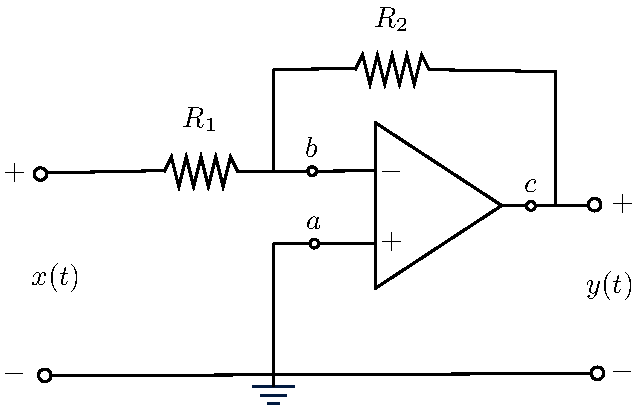
\includegraphics[width=3in]{plots/multiplierbadri1.pdf}
\captionof{figure}{The circuit}
 \label{Fig-Prob2.1a}
}

To simplify the circuit, one has to use the model for the opamp given in Fig.~\ref{Fig-Prob2.1b} which involves the voltage-controlled voltage-source (VCVS) at the output side (indicated in green).  While replacing the operational amplifier with its model, it must be noted that the positive terminal of the operational amplifier is connected to the ground.

{
\centering 
\captionsetup{type=figure}
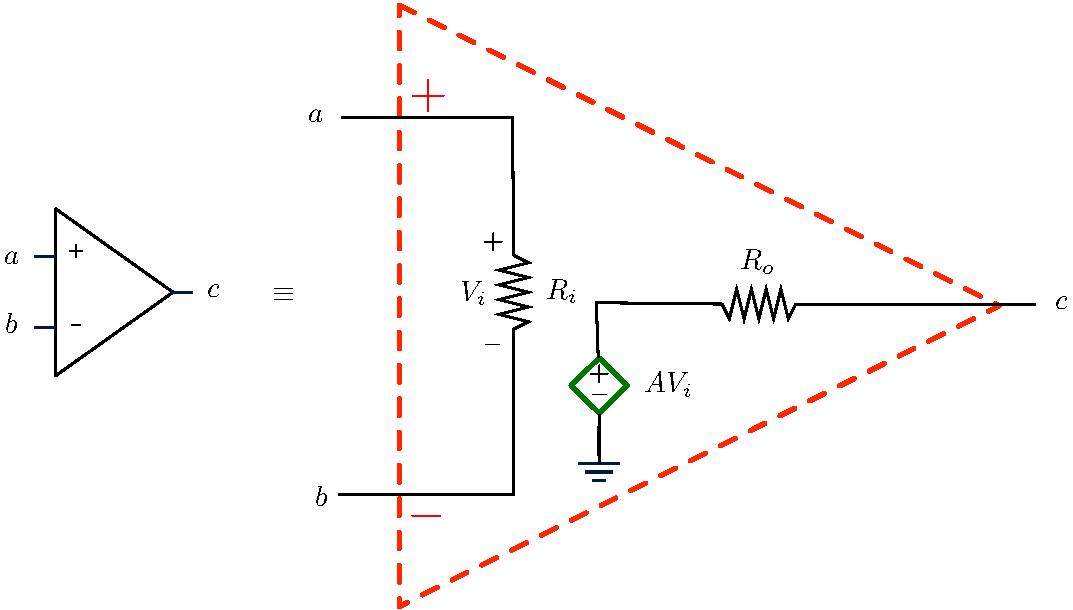
\includegraphics[width=5in]{plots/multiplierbadri2.pdf}
\captionof{figure}{The model for an operational amplifier}
 \label{Fig-Prob2.1b}
}

Upon replacement, we obtain the following equivalent circuit. Again notice that since the positive terminal of the opamp was connected to the ground, the voltage output by the VCVS is $AV_i$ where $V_i$ is the voltage between the ground and the top of the resistance $R_i$, and is measured against the flow of the current $i-i_1$ as is indicated in the figure.

{
\centering 
\captionsetup{type=figure}
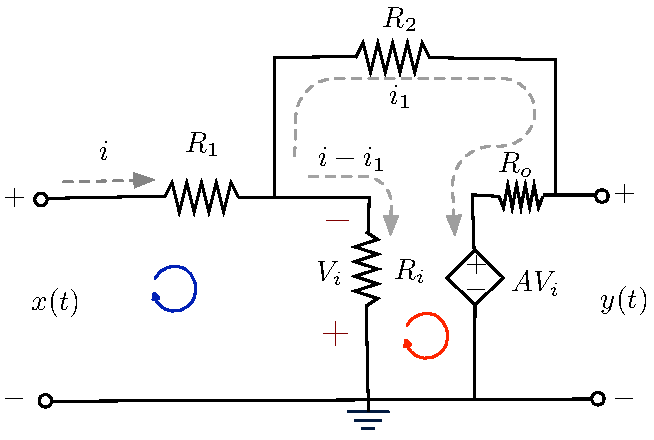
\includegraphics[width=4in]{plots/multiplierbadri3.pdf}
\captionof{figure}{The operational amplifier circuit with the model}
 \label{Fig-Prob2.1c}
}

Applying Kirchoff's law to the outer loop indicated in blue in Fig.~\ref{Fig-Prob2.1c}, we obtain the following equation.
\begin{equation}
x(t) = iR_1+(i-i_1)R_i = i(R_1+R_i) - i_1 R \label{eqn-Prob2.1.1}
\end{equation}
Note that by definition, the voltage $V_i$ that controls the VCVS is the voltage across $R_i$ measured against the indicated direction of the current $i-i_1$, and is given by
\begin{equation}
V_i = -(i-i_1)R_i. \label{eqn-Prob2.1.2}
\end{equation}
Next, writing out the Kirchoff's law for the inner loop indicated in red, we obtain the following.
\begin{align}
0 &= i_1 R_2 + i_2 R_0 + AV_i - (i-i_1) R_i
\end{align}
Substituting $V_i$ in the above equation with the RHS of \eqref{eqn-Prob2.1.2}, we obtain the following.
\begin{align}
0&= i_1 (R_2+R_0) - A(i-i_1)R_i-(i-i_1)R_i\\
&= -i(1+A)R_i+i_1((1+A)R_i+R_0+R_2)\label{eqn-Prob2.1.3}
\end{align}
Combining \eqref{eqn-Prob2.1.3} and \eqref{eqn-Prob2.1.1}, we obtain the following linear system of equations governing the electrical circuit.
\begin{align}
\left[\begin{array}{cc} R_1+R_i &  -R_i\\ -(1+A)R_i & (1+A)R_i+R_0+R_2\end{array}\right]\left[\begin{array}{c} i\\ i_1\end{array}\right] = \left[\begin{array}{c} x(t)\\ 0\end{array}\right]
\end{align}
Solving the above linear system, we identify the current in the different branches to be
\begin{align}
\left[\begin{array}{c} i\\ i_1\end{array}\right] = x(t)\left[\begin{array}{c} \frac{ (1+A)R_i+R_0+R_2}{(1+A) R_iR_1+R_0R_1+R_2R_1+R_0R_i+R_2R_i}\\ \frac{(1+A)R_i}{(1+A) R_iR_1+R_0R_1+R_2R_1+R_0R_i+R_2R_i}\end{array}\right].\label{eqn-Prob2.1.4}
\end{align}
Lastly, notice that
\begin{align}
y(t) &= i_1 R_0 + A V_i \\
 & = i_1 R_0 - (i-i_1)R_i.
\end{align}
Substituting the solutions for $i$ and $i_1$ in terms of $x(t)$, we obtain the following.
\begin{align}
y(t)= \left( \frac{R_iR_0 - R_2R_iA}{(1+A) R_iR_1+R_0R_1+R_2R_1+R_0R_i+R_2R_i} \right)x(t)
\end{align}


\end{solution}

\end{excersizelist}


%\clearpage
\chapter{Linear time invariant systems}\label{sec:prop-line-time}

In the previous section we derived differential equations that model mechanical, electrical, and electro-mechanical systems.  The equations themselves often do not provide as much information about these system as we require.  For example, we were able to find a signal $p$ representing the position of the mass-spring-damper in Figure~\ref{mech:massspring1} given a particular force signal $f$ is applied to the mass.  However, it is not immediately obvious how to find the force signal $f$ given a particular position signal $p$.  We will be able to solve this problem and, more generally, to describe properties of systems modelled by linear differential equations with constant coefficient, if we make the added assumptions that the systems are \term{linear} and \term{time invariant}.  We study linear time invariant systems in this chapter.  Throughout this chapter $H$ will denote a linear time invariant system.

\section{Convolution, regular systems and the delta ``function''} \label{sec:conv-regul-syst}

A large number of linear time invariant systems can be represented by a signal called the \term{impulse response}.  The impulse response of a system $H$ is a signal $h$ such that
\[
H(x,t) = \int_{-\infty}^{\infty} h(\tau) x(t - \tau) d\tau,
\]
that is, the response of $H$ to input signal $x$ can be represented as an integral equation involving $x$ and the impulse response $h$.  The integral is called a \term{convolution} and appears so often that a special notation is used for it.  We write $h * x$ to  indicate the signal that results from convolution of signals $h$ and $x$, that is, $h * x$ is the signal satisfying
\[
h * x = \int_{-\infty}^{\infty} h(\tau) x(t - \tau) d\tau.
\]
%where $(h*x)(t)$ indicates $h*x$ evaluated at $t$.  
Those systems that have an impulse response we call \term{regular systems}\footnote{The name \term{regular system} is motivated by the term \term{regular distribution}~\citep{Zemanian_dist_theory_1965}}.  Observe that regular systems are linear because
\begin{equation}\begin{split}\label{eq:regsystemislinear}
H(ax + by) &= h * (ax + by) \\
&= \int_{-\infty}^{\infty} h(\tau) \big(ax(t - \tau) + by(t - \tau)\big) d\tau \\
&= a\int_{-\infty}^{\infty} h(\tau) x(t - \tau) d\tau + b\int_{-\infty}^{\infty} h(\tau)y(t - \tau) d\tau \\
&= a (h * x) + b(h*y) \\
&= a H(x) + bH(y).
\end{split}\end{equation}
The above equations show that convolution commutes with scalar multiplication and distributes with addition, that is,
\[
h * (ax + by) =  a (h * x) + b(h*y).
\]
Regular systems are also time invariant because
\begin{align*}
T_\kappa\big(H(x)\big) &= T_\kappa(h * x ) \\
&= \int_{-\infty}^{\infty} h(\tau) x(t- \kappa - \tau) d\tau \\
&= \int_{-\infty}^{\infty} h(\tau) T_\kappa(x, t - \tau) d\tau \\ 
&= h * T_\kappa(x) \\
&= H\big(T_\kappa(x)\big). 
\end{align*}

We can define the impulse response of a regular system $H$ in the following way.  First define the signal
\[
p_\gamma(t) = \begin{cases}
\gamma, & 0 < t \leq \frac{1}{\gamma} \\
0, & \text{otherwise},
\end{cases}
\]
that is, a rectangular shaped pulse of height $\gamma$ and width $\tfrac{1}{\gamma}$.  The signal $p_\gamma$ is plotted in Figure~\ref{fig:rectpulsedelta} for $\gamma=\frac{1}{2},1,2,5$.  As $\gamma$ increases the pulse gets thinner and higher so as to keep the area under $p_\gamma$ equal to one.  Consider the response of the regular system $H$ to the signal $p_\gamma$,
\begin{align*}
H(p_\gamma) &= h * p_\gamma \\
&= \int_{-\infty}^\infty h(\tau) p_\gamma(t - \tau) d\tau \\
&= \gamma \int_{t- 1/\gamma}^{t} h(\tau) d\tau.
\end{align*}
Taking limits as $\gamma\rightarrow\infty$,
\[
\lim_{\gamma \rightarrow \infty} H(p_\gamma) = \lim_{\gamma \rightarrow \infty} \gamma \int_{t- 1/\gamma}^{t} h(\tau) d\tau = h(t) \;\; \text{a.e.}
\]
Thus, we define the impulse response of a regular system $H$ as the limit  
\begin{equation}\label{eq:defnimpulseresponse}
h = \lim_{\gamma \rightarrow \infty} H(p_\gamma).  
\end{equation}
The limit exists when $H$ is regular.  If this limit does not exist, the system is not regular and does not have an impulse response.  %The reader unclear on the meaning of the limit above might want to review Section~\ref{sec:convergence-signals}.

%BLERG Young's inequality gives a neat way of knowing when convolutions exist or don't exists based on what Lp space the signals lie in.  This becomes useful in the Fourier transform section?

As an example, consider the integrator system
\begin{equation}\label{eq:integratorforfigref}
I_\infty(x) = \int_{-\infty}^{t} x(\tau) d\tau
\end{equation}
described in Section~\ref{sec:some-import-syst}.  This systems response to $p_\gamma$ is 
\[
I_\infty(p_\gamma,t) = \int_{-\infty}^{t} p_\gamma(\tau) d\tau = \begin{cases}
0, & t \leq 0 \\
\gamma t, & 0 < t \leq \frac{1}{\gamma} \\
1, & t > \frac{1}{\gamma}
\end{cases}
\]
The response is plotted in Figure~\ref{fig:rectpulsedelta}.  Taking the limit as $\gamma \rightarrow\infty$ we find that the impulse response of the integrator is the step function
\begin{equation}\label{eq:utimprespstep}
u(t) = \lim_{\gamma\rightarrow\infty} H(p_\gamma) = \begin{cases}
0 & t \leq 0 \\
1 & t > 0.
\end{cases} \qquad \text{a.e.}
\end{equation}

\newcommand{\rectpulse}[1]{\draw[color=black,thick] (-0.5,0) -- (0,0) -- (0,#1) -- (1.0/#1,#1) node[right] {$\gamma=#1$}-- (1.0/#1,0) -- (3,0)}
\newcommand{\pulseresponse}[2]{\draw[color=black,thick] (-0.5,0) -- (0,0) -- node [rotate=atan(#1),pos=#2,below] {$\gamma=#1$} (4*1.0/#1,4*1) -- (4*5,4*1)}
\begin{figure}[tp]
  \centering
  \begin{tikzpicture}
    % \draw[very thin,color=gray] (-0.1,-1.1) grid (3.9,3.9);
    \draw[->] (-0.75,0) -- (3.5,0) node[above] {$t$};
    \draw[->] (0,-0.5) -- (0,5.5) node[right] {$p_\gamma(t)$};
    \rectpulse{1.0};
    \rectpulse{5.0};
    \rectpulse{2.0};
    \rectpulse{0.5};
    \vtick{1.0} node[pos=0.5,below] {$1$};
    \vtick{2.0} node[pos=0.5,below] {$2$};
    \htick{1.0} node[pos=0.5,left] {$1$};
    \htick{2.0} node[pos=0.5,left] {$2$};
    \htick{5.0} node[pos=0.5,left] {$5$};
  \end{tikzpicture}
\;\;
  \begin{tikzpicture}
    % \draw[very thin,color=gray] (-0.1,-1.1) grid (3.9,3.9);
    \draw[->] (-0.75,0) -- (5.5,0) node[above] {$t$};
    \draw[->] (0,-0.5) -- (0,5.5) node[right] {$I_\infty(p_\gamma,t)$};
    \begin{scope}[font=\small]
      \clip (0,0) rectangle (5,5);
      \pulseresponse{5.0}{0.75};
      \pulseresponse{2.0}{0.7};
      \pulseresponse{1.0}{0.6};
      \pulseresponse{0.5}{0.4};
    \end{scope}
    \draw[color=black,thick] (-0.5,0) -- (0,0) -- node[rotate=90,pos=0.6,above] {$\gamma=\infty$} (0,4) -- (5,4);
    \htick{4.0} node[pos=0.5,left] {$1$};
    \vtick{2.0} node[pos=0.5,below] {$0.5$};
    \vtick{4.0} node[pos=0.5,below] {$1$};
  \end{tikzpicture}
  \caption{The rectangular shaped pulse $p_\gamma$ for $\gamma=0.5,1,2,5$ and the response of the integrator~\eqref{eq:integratorforfigref} to $p_\gamma$ for $\gamma=0.5,1,2,5,\infty$.} \label{fig:rectpulsedelta}
\end{figure}

Some important systems do not have an impulse response.  For example, the identity system $T_0$ does not because
\[
\lim_{\gamma \rightarrow \infty} T_0(p_\gamma) = \lim_{\gamma \rightarrow \infty} p_\gamma
\]
does not exist.  %BLERG what is this all about actually?  Is is something like.  The convergence is not ``almost everywhere''?
Similarly, all the time shifters $T_\tau$ do not have impulse responses.  However, it can be notationally useful to pretend that $T_0$ \emph{does} have an impulse response and we denote it by the symbol $\delta$ called the \term{delta function}.  The idea is to assign $\delta$ the property
\[
\int_{-\infty}^\infty x(t) \delta(t) dt = x(0) %= \lim_{\gamma \rightarrow \infty}\int_{\infty}^\infty x(t) p_\gamma(t) dt
\]
so that convolution of $x$ and $\delta$ satisfies
\[
\delta * x = \int_{-\infty}^{\infty} \delta(\tau) x(t - \tau) d\tau = x(t) = T_0(x).
\]
We now treat $\delta$ as if it were a signal.  So $\delta(t - \tau)$ will represent the impulse response of the time shifter $T_\tau$ because
\begin{align*}
T_\tau(x) &= \delta(t - \tau) * x \\
&= \int_{-\infty}^{\infty} \delta(\kappa -\tau) x(t - \kappa) d\kappa \\
&= \int_{-\infty}^{\infty} \delta(k) x(t - \tau - k) dk & \text{(change variable $k = \kappa - \tau$)}\\
&= x(t-\tau).
\end{align*}
For $a\in \reals$ it is common to plot $a\delta(t - \tau)$ using an arrow of height $a$ at $t = \tau$ as indicated in Figure~\ref{fig:deltafuncplotexample}.  It is important to realise that $\delta$ is not actually a signal.  It is not a function.  However, it can be convenient to treat $\delta$ as if it were a function.  The manipulations in the last set of equations, such as the change of variables, are not formally justified, but they do lead to the desired result $T_\tau(x) = x(t-\tau)$ in this case.  In general, there is no guarantee that mechanical mathematical manipulations involving $\delta$ will lead to sensible results.

\begin{figure}[tp]
\centering
\begin{tikzpicture}[domain=-2.4:2.4,samples=100]
    %\draw[very thin,color=gray] (-0.1,-1.1) grid (3.9,3.9);
    \draw[->] (-2.8,0) -- (2.8,0) node[above] {$t$};
    \draw[->] (0,-2.4) -- (0,2.4) node[above] {$\delta(t+2) + 2\delta(t) - \delta(t-1)$};
    \draw[->,thick,>=latex] (0,0) -- (0,2);
    \draw[->,thick,>=latex] (1,0) -- (1,1);
    \draw[->,thick,>=latex] (-2,0) -- (-2,-1);
    \htick{1} node[pos=0.5,left] {$1$};
    %\htick{-1} node[pos=0.5,right] {$-1$}; 
    %\vtick{-2} node[pos=0.5,above] {$-2$};
    \vtick{-1} node[pos=0.5,below] {$-1$};
    %\vtick{1} node[pos=0.5,below] {$1$};
    \vtick{2} node[pos=0.5,below] {$2$};

    % \draw[color=black] plot[id=x] function{1/x^2} 
    %    node[right] {$f(t) = t^{-2}$};
    %\draw[smooth,color=black,thick] plot function{sin(3.14159265359*x)};
    %\draw[color=black] plot[id=exp] function{0.05*exp(x)} 
    %    node[right] {$f(t) = \frac{1}{20} e^t$};
\end{tikzpicture} 
\;\;
\begin{tikzpicture}[domain=-2.4:2.4,samples=100]
    %\draw[very thin,color=gray] (-0.1,-1.1) grid (3.9,3.9);
    \draw[->] (-2.8,0) -- (2.8,0) node[above] {$t$};
    \draw[->] (0,-2.4) -- (0,2.4) node[above] {$2\sin(\pi t) + \delta(t - \tfrac{3}{2})$};
    \draw[smooth,color=black,thick] plot function{2*sin(3.14159265359*x)};
    \draw[->,thick,>=latex] (pi/2,0) -- (pi/2,1);
    \htick{2} node[pos=0.5,left] {$2$};
    %\htick{-1} node[pos=0.5,right] {$-1$}; 
    %\vtick{-2} node[pos=0.5,above] {$-2$};
    %\vtick{-1} node[pos=0.5,below] {$-1$};
    %\vtick{1} node[pos=0.5,below] {$1$};
    \vtick{1/2} node[pos=0.5,below] {$\tfrac{1}{2}$};
    % \draw[color=black] plot[id=exp] function{0.05*exp(x)} 
    %    node[right] {$f(t) = \frac{1}{20} e^t$};
\end{tikzpicture} 
\caption{Plot of the ``signal'' $\delta(t+2) + 2\delta(t) - \delta(t-1)$ (left) and the ``signal'' $2\sin(\pi t) + \delta(t - \tfrac{3}{2})$ (right).} \label{fig:deltafuncplotexample}
\end{figure}

The only other non regular systems that we have use of are differentiators $D^k$, and it is convenient to define a similar notation for pretending that these systems have an impulse response.  In this case we use the symbol $\delta^k$ and assign it the property
\[
\int_{-\infty}^\infty x(t) \delta^k(t) dt = D^k(x,0),
\]
so that convolution of $x$ and $\delta$ is
\[
\delta^k * x = \int_{-\infty}^{\infty} \delta^k(\tau) x(t - \tau) d\tau = D^k(x,t).
\]
As with the delta function the symbol $\delta^k$ must be treated with care.  This notation can be useful, but purely formal manipulations with $\delta^k$ may not lead to sensible results in general.

% The pulse $p_\gamma(t)$ is not differentiable at $t = 0$ and $t=\tfrac{1}{\gamma}$.  Fortunately $\{ p_\gamma, \gamma \in \reals\}$ is not the only family that can be used to define the impulse response.  It is instructive, and useful to instead use a family that is \term{infinately differentiable} (can be differentiated as many times as we like).  An example of such a family is
% \[
% \delta_\gamma = \begin{cases}

% \end{cases}
% \] 

The impulse response $h$ immediately yields some properties of the corresponding system $H$.  For example, if $h(t) = 0$ for all $t < 0$, then $H$ is causal because 
\[
H(x) = h * x =  \int_{-\infty}^{\infty} h(\tau) x(t - \tau) d\tau = \int_{0}^{\infty} h(\tau) x(t - \tau) d\tau
\] 
only depends on values of the input signal $x$ at times less than $t$, i.e., only times $t - \tau$ with $\tau > 0$.  The system $H$ is stable if and only if $h$ is absolutely integrable (Exercise~\ref{excer:bibostableimpulseresp}).

Another important signal is the \term{step response} of a system that is defined as the response of the system to the step function $u(t)$.  For example, the step response of the time shifter $T_\tau$ is the time shifted step function $T_\tau(u,t) = u(t - \tau)$.  The step response of the integrator $I_\infty$ is
\[
I_\infty(u) = \int_{-\infty}^t u(\tau) d\tau = \begin{cases}
\int_{0}^t d\tau  = t & t > 0 \\
0 & t \leq 0.
\end{cases}
\]
This signal is often called the \term{ramp function}.  Not all systems have a step response.  For example, the system with impulse response $u(-t)$ does not because the convolution of the step $u(t)$ and its reflection $u(-t)$ does not exist.  If a system $H$ has both an impulse response $h$ and a step response $H(u)$, then these two signals are related.  To see this, observe that the step response is
\begin{equation}\label{eq:stepresponseintegrateimpulseresponse}
H(u) = h * u = \int_{-\infty}^{\infty}h(\tau)u(t - \tau) d\tau = \int_{-\infty}^{t} h(\tau) d\tau = I_\infty(h). 
\end{equation}
Thus, the step response can be obtained by applying the integrator $I_\infty$ to the impulse response.

\section{Properties of convolution}\label{sec:prop-conv}

The convolution $x * y$ of two signals $x$ and $y$ does not always exist.  For example, if $x(t) = u(t)$ and $y(t) = 1$, then
\[
x * y = \int_{-\infty}^\infty x(\tau) y(t - \tau) d\tau = \int_{-\infty}^\infty u(\tau) d\tau = \int_{0}^\infty d\tau
\]
is not finite for any $t$.  We cannot convolve the step function $u$ and the signal that is equal to $1$ for all time.  On the other hand, if $x(t) = y(t) = u(t)$, then
\[
x * y = \int_{-\infty}^\infty u(\tau) u(t - \tau) d\tau =  \begin{cases}
\int_{0}^t d\tau  = \tau & t > 0 \\
0 & t \leq 0,
\end{cases}
\]
if finite for all $t$.  % The convolution $x * y$ always exists if both $x$ and $y$ are right sided because, in this case, there exists a $T \in \reals$ such that $x(t) = y(t) = 0$ for all $t < T$, and so
% \[
% z(t) = x * y = \int_{-\infty}^\infty x(\tau) y(t - \tau) d\tau = \int_{t-T}^Tx(\tau) y(t - \tau) d\tau.
% \]
% This integral exists because both $x$ and $y$ are locally integrable (see Section~\ref{sec:properties-signals}).  Similarly $x*y$ exists if both $x$ and $y$ are left sided or if one of $x$ or $y$ is finite.

We have already shown in~\eqref{eq:regsystemislinear} that convolution commutes with scalar multiplication and is distributive with addition, that is, for signals $x,y,w$ and complex numbers $a,b$,
\[
a (x * w) + b (y * w) = (ax + by) * w.
\]

Convolution is commutative, that is, $x*y = y*x$ whenever these convolutions exist.  To see this, write
\begin{align*}
x*y &= \int_{-\infty}^\infty x(\tau) y(t - \tau) d\tau \\
&= \int_{-\infty}^\infty x(t - \kappa) y(\kappa) d\kappa \qquad (\text{change variable $\kappa = t - \tau$}) \\
&= y * x.
\end{align*}
Convolution is also associative, that is, for signals $x,y,z$, 
\[
(x*y)*z = x*(y*z). \qquad \text{(see Exercise~\ref{excer:convassociative})}
\]
By combining the associative and commutative properties we find that the order in which the convolutions in $x * y * z$ are performed does not mater, that is
\[
x*y*z = y*z*x = z*x*y = y*x*z = x*z*y = z*y*x
\]
provided that all the convolutions involved exist.  More generally, the order in which any sequence of convolutions is performed does not change the final result.

\section{Linear combining and composition}\label{sec:line-comb-comp}

Let $H_1$ and $H_2$ be linear time invariant systems and let $H$ be the system
\[
H(x) = cH_1(x) + dH_2(x), \qquad c,d \in \complex
\]
formed by a linear combination of $H_1$ and $H_2$.  The system $H$ is linear because for signals $x,y$ and complex numbers $a,b$,
\begin{align*}
H(ax + by) &= cH_1(ax+by) + dH_2(ax+by) \\
&= acH_1(x)+bcH_1(y) + adH_2(x)+ bdH_2(y) & \text{(linearity $H_1, H_2$)} \\
&= a\big( cH_1(x)  + dH_2(x) \big) + b\big( cH_1(y) + dH_2(y) \big) \\
&= aH(x) + bH(y).
\end{align*}
The system is also time invariant because
\begin{align*}
H\big(T_\tau(x)\big) &= cH_1\big(T_\tau(x)\big) + dH_2\big(T_\tau(x)\big)  \\
&= c T_\tau\big( H_1(x)\big) + dT_\tau\big(H_2(x)\big) & \text{(time-invariance $H_1,H_2$)} \\
&= T_\tau\big( cH_1(x) + dH_2(x)\big) & \text{(linearity $T_\tau$)} \\
&= T_\tau\big(H(x)\big).
\end{align*}
So, we can construct linear time invariant systems by \term{linearly combining} (adding and multiplying by constants) other linear time invariant systems.  If $H_1$ and $H_2$ are regular systems this linear combining property can be expressed using their impulse responses $h_1$ and $h_2$.  We have
\begin{align*}
H(x) &= a H_1(x) + b H_2(x) \\
&= a h_1 * x + b h_2 * x \\
&= (a h_1 + bh_2) * x &\text{(distributivity of convolution)}\\
&= h * x,
\end{align*}
and so, $H$ is a regular system with impulse response $h = ah_1 + bh_2$.  %Thus, if $H$ is the linear combination of $H_1$ and $H_2$, then the impulse response of $H$ is the same linear combination of the impulse responses of $H_1$ and $H_2$.

\begin{figure}
\centering
\begin{tikzpicture}[node distance=1.5cm,auto,>=latex']
    \node[dspadder] (adder) {};
    \node [dspnodeopen] (res) [right of=adder,node distance=1.5cm,label=right:{$H(x)=cH_1(x)+dH_2(x)$}] {};
    \node[dspmixer,dsp/label=right] (amult) [above of=adder,node distance=1cm] {$c$};
    \node [dspsquare] (H1) [left of=amult] {$H_1$};
    \node[dspmixer,dsp/label=right] (bmult) [below of=adder,node distance=1cm] {$d$};
    \node [dspsquare] (H2) [left of=bmult] {$H_2$};
     \node [dspnodeopen] (x) [left of=adder,node distance=3cm,label=left:$x$] {};
   
     \draw[dspflow] (x) -- ($ (H1) !.5! (H2) $);
     \draw[dspconn] ($ (H1) !.5! (H2) $) -- (H2);
     \draw[dspconn] ($ (H1) !.5! (H2) $) -- (H1);
     \draw[dspconn] (H1) -- (amult);
     \draw[dspconn] (H2) -- (bmult);
    \draw[dspconn] (amult) -- (adder);
    \draw[dspconn] (bmult) -- (adder);
    \draw[dspflow] (adder) -- (res);
    
    \node (H) at (-0.7,0) [draw,thick,dashed,minimum width=3.5cm,minimum height=3cm,label=above:$H$] {};
    
\end{tikzpicture}
\caption{Block diagram depicting the linear combining property of linear time invariant systems. The system $cH_1(x)+dH_2(x)$ can be expressed as a single linear time invariant system $H(x)$.}\label{blockdiag:lineartisystem}
\end{figure}


Another way to construct linear time invariant systems is by \term{composition}.  Let $H_1$ and $H_2$ be linear time invariant systems and let
\[
H(x) = H_2\big(H_1(x)\big),
\]
that is, $H$ first applies the system $H_1$ and then applies the system $H_2$.  The composition $H_2\big(H_1(x)\big)$ only applies to those signals $x$ in the domain of $H_1$ and such that the signal $H_1(x)$ is in the domain of $H_2$.  The system $H$ is linear because, for signals $x,y$ and complex numbers $a,b$,
\begin{align*}
H(ax + by) &= H_2\big(H_1(ax + by)\big) \\
&= H_2\big(aH_1(x) + bH_1(y)\big)  &\text{(linearity $H_1$)}\\
&= aH_2\big(H_1(x)) + bH_2\big(H_1(y))\big)  &\text{(linearity $H_2$)} \\
&= aH(x) + bH(y).
\end{align*}
The system is also time invariant because
\begin{align*}
H\big(T_\tau(x)\big) &= H_2\big(H_1(T_\tau(x)\big) \\
&= H_2\big(T_\tau\big(H_1(x)\big)\big)  &\text{(time-invariance $H_1$)}\\
&= T_\tau\big(H_2\big(H_1(x)\big)\big)  &\text{(time-invariance $H_2$)} \\
&= T_\tau\big(H(x)\big).
\end{align*}
If $H_1$ and $H_2$ are regular systems the composition property can be expressed using their impulse responses $h_1$ and $h_2$.  It follows that
\begin{align*}
H(x) &= H_2(H_1(x)) \\
&= h_2 * (h_1 * x) \\
&= (h_2* h_1) * x &\text{(associativity of convolution)} \\
&= h * x,
\end{align*}
and so, $H$ is a regular system with impulse response $h = h_2 * h_1$.  %Thus, if $H$ is the composition of regular systems $H_1$ and $H_2$, then $H$ is a regular system with impulse given by the convolution of the impulse responses of $H_1$ and $H_2$.  %On the third line in the equation above we have use the associativity of convolution (Excersize~\ref{excer:convassociative}).

\begin{figure}
\centering
\begin{tikzpicture}[node distance=1.5cm,auto,>=latex']
    \node[dspnodeopen] (x) [label=left:{$x$}] {};
    \node [dspsquare] (H1) [right of=x] {$H_1$};
    \node [dspsquare] (H2) [right of=H1] {$H_2$};
    \node[dspnodeopen] (res) [right of=H2,label=right:{$H(x)=H_2(H_1(x))$}] {};
    \draw[dspconn] (x) -- (H1);
    \draw[dspconn] (H1) -- (H2);
    \draw[dspflow] (H2) -- (res);
    
    \node (H) at ($ (x) !.5! (res) $) [draw,thick,dashed,minimum width=3cm,minimum height=1.5cm,label=above:$H$] {};
    
\end{tikzpicture}
\caption{Block diagram depicting the composition property of linear time invariant systems. The system $H_2(H_1(x))$ can be expressed as a single linear time invariant system $H(x)$.}\label{blockdiag:compositionlti}
\end{figure}

A wide variety of linear time invariant systems can now be constructed by linearly combining and composing simpler systems.  

% \section{Commutative (sometimes)}
% %\section{Commutative and invertible (sometimes)}

% Let $H$ and $G$ be regular systems with impulse response $h$ and $g$.  If $h$ and $g$ can be convolved then $h*g = g*h$ and the corresponding systems $H$ and $G$ commute, that is
% \[
% H\big(G(x)\big) = h * g * x = g * h * x = G\big(H(x)\big),
% \]
% whenever the convolutions involved exist.  This commutative property is depicted by the block diagram in Figure~\ref{blockdiag:commutativesystems}.

% The commutative property is very useful when it holds.  It allows us to construct large systems by composing smaller systems without concern for the order in which systems are composed.  However, linear time invariant systems do not always commute, and so, some care must be taken.  For example, applying a differentiator $D$ followed by the integrator $I_\infty$ to the signal $x(t) = 1$ gives
% \[
% I_\infty\big( D(x), t) = I_0\big( 0 , t) = 0 \qquad \text{for all $t$}
% \] 
% because $D(x,t) = 0$ for all $t$.  However, applying the integrator to $x$ gives
% \[
% I_\infty(x, t) = \int_{-\infty}^t dt = \infty 
% \]
% which does not exists, and so $D(I_0(x),t)$ does not exist.  In the previous example problems arise because the signal $x(t) = 1$ is in the domain 
% %(more specifically the \term{null space}) 
% of the differentiator $D$, but it is not in the domain of the integrator $I_\infty$.  We will be able to more precisely specify conditions under which linear time invariant systems commute when we introduce the Laplace transform in Section~\ref{sec:laplace-transform}.

% Many linear time invariant systems are invertible, for example, the inverse of the time shifter $T_\tau$ is $T_{-\tau}$  and, by the fundamental theorem of calculus, the inverse of the integrator $I_\infty$ is the differentiator.  Consider the system
% \[
% H(x,t) = x(t) + x(t - 1).
% \]
% We can guess its inverse to be
% \[
% H^{-1}(x,t) = 
% \]
% In Section~\ref{sec:laplace-transform} we will use the Laplace transform to construct the inverse of some regular systems.  Not all linear time invariant systems are invertible.  For example, 

%BLERG: YOU CAN SPECIFY WHEN THEY ARE INVERTIBLE ONCE YOU HAVE THE FOURIER TRANSFORM

%BLERG: YOU CAN SPECIFY WHEN THEY WILL COMUTE ONCE YOU HAVE THE LAPLACE TRANSFORM

%BLERG: Add a test where you concatenate two circuits. The two masses, and spring and a damper system might give some interesting insight into commutivity.

% \begin{figure}[tbp]
% \centering
% \begin{tikzpicture}[node distance=1.3cm,auto,>=latex']
%     \node[dspnodeopen,dsp/label=above] (x) {$x$};
%     \node[dspsquare] (H) [right of=x] {$H$};
%     \node[dspsquare] (D) [right of=H] {$G$};  
%     \node[dspnodeopen,dsp/label=above] (out) [right of=D,node distance=1.7cm,label=above:$H\big(G(x)\big)$] {};
%     \draw[dspconn] (x) -- (H);
%     \draw[dspconn] (H) -- (D);
%     \draw[dspflow] (D) -- (out);
% \end{tikzpicture}
% \qquad
% \begin{tikzpicture}[node distance=1.3cm,auto,>=latex']
%   \node[dspnodeopen,dsp/label=above] (x) {$x$};
%   \node[dspsquare] (D) [right of=x] {$G$};  
%   \node[dspsquare] (H) [right of=D] {$H$};
%   \node[dspnodeopen,dsp/label=above] (out) [right of=H,node distance=1.7cm,label=above:$G\big(H(x)\big)$] {};
%   \draw[dspconn] (x) -- (D);
%   \draw[dspconn] (D) -- (H);
%   \draw[dspflow] (H) -- (out);
% \end{tikzpicture}
% \caption{If $H$ and $G$ commute the outputs of these two diagrams are the same, that is, $H\big(G(x)\big) = G\big(H(x)\big)$.}\label{blockdiag:commutativesystems}
% \end{figure}


\section{Eigenfunctions and the transfer function}\label{sec:eigenf-line-time}

\begin{figure}[p]
\centering
\begin{tikzpicture}[domain=-1:9,samples=200]
    %\draw[very thin,color=gray] (-0.1,-1.1) grid (3.9,3.9);
\begin{scope}[yscale=1]
    \draw[->] (-1.5,0) -- (10,0) node[above] {$t$};
    \draw[->] (0,-2.8) -- (0,2.8) node[right] {$\cos(\pi t) e^{\sigma t}$};
    %\draw[smooth,color=black,thick] plot function{sin(3.14159265359*x)*exp(-x)};
    \draw[smooth,color=black,thick] plot function{cos(3.14159265359*x)};
    \draw[smooth,color=black,thick] plot function{cos(3.14159265359*x)*exp(x/10)};
    \draw[smooth,color=black,thick] plot function{cos(3.14159265359*x)*exp(-x/10)};
    \draw[smooth,color=black,dashed] plot function{exp(x/10)};
    \draw[smooth,color=black,dashed] plot function{exp(-x/10)};
    \draw[smooth,color=black,dashed] plot function{-exp(x/10)};
    \draw[smooth,color=black,dashed] plot function{-exp(-x/10)};
    \node at (9.3,-1) {$0$};
    \node at (6,-0.85) {$-e^{-\frac{1}{10}}$};
    \node at (6,-2.2) {$-e^{\frac{1}{10}}$};
    \node at (7.1,2.3) {$e^{\frac{1}{10}}$};
    \node at (7.1,0.8) {$e^{-\frac{1}{10}}$};
    \htick{2} node[pos=0.5,left] {$2$};
    \htick{-2} node[pos=0.5,left] {$-2$};
\end{scope}
\end{tikzpicture}

\vspace{1cm}
\begin{tikzpicture}[domain=-1:9,samples=200]
    %\draw[very thin,color=gray] (-0.1,-1.1) grid (3.9,3.9);
\begin{scope}[yscale=1]
    \draw[->] (-1.5,0) -- (10,0) node[above] {$t$};
    \draw[->] (0,-2.8) -- (0,2.8) node[right] {$\sin(\pi t) e^{\sigma t}$};
    %\draw[smooth,color=black,thick] plot function{sin(3.14159265359*x)*exp(-x)};
    \draw[smooth,color=black,thick] plot function{sin(3.14159265359*x)};
    \draw[smooth,color=black,thick] plot function{sin(3.14159265359*x)*exp(x/10)};
    \draw[smooth,color=black,thick] plot function{sin(3.14159265359*x)*exp(-x/10)};
    \draw[smooth,color=black,dashed] plot function{exp(x/10)};
    \draw[smooth,color=black,dashed] plot function{exp(-x/10)};
    \draw[smooth,color=black,dashed] plot function{-exp(x/10)};
    \draw[smooth,color=black,dashed] plot function{-exp(-x/10)};
    \node at (9.3,-1) {$0$};
    \node at (6.5,-0.85) {$-e^{-\frac{1}{10}}$};
    \node at (6.5,-2.3) {$-e^{\frac{1}{10}}$};
    \node at (7.5,2.45) {$e^{\frac{1}{10}}$};
    \node at (7.5,0.75) {$e^{-\frac{1}{10}}$};
    \htick{2} node[pos=0.5,left] {$2$};
    \htick{-2} node[pos=0.5,left] {$-2$};
\end{scope}
\end{tikzpicture}
\caption{The function $\cos(\pi t) e^{\sigma t}$ (top) and $\sin(\pi t) e^{\sigma t}$ (bottom) for $\sigma = -\tfrac{1}{10},0,\tfrac{1}{10}$.} 
\label{fig:sinabsdecay}
\end{figure}


Let $s = \sigma + j \omega \in \complex$.  Complex exponential signals of the form 
\[
e^{st} = e^{\sigma t}e^{j \omega t} = e^{\sigma t} \big( \cos(\omega t) + j \sin(\omega t) \big)
\]
play an important role in the study of linear time invariant systems.  The real and imaginary parts of the signal $e^{(\sigma + j\pi)t}$ with $\sigma = -\tfrac{1}{10},0,\tfrac{1}{10}$ are plotted in Figure~\ref{fig:sinabsdecay}.  The signal is oscillatory when $\omega \neq 0$.  The signal converges to zero as $t\to\infty$ when $\sigma<0$ and diverges as $t\to\infty$ when $\sigma > 0$.  

Let $H$ be a linear time invariant system and let $y = H(e^{st})$ be the response of $H$ to the exponential signal $e^{st}$.  Consider the response of $H$ to the time-shifted signal $e^{s(t+\tau)}$ for $\tau \in \reals$.  By time-invariance
\[
H(e^{s(t+\tau)},t) = H(e^{st}, t+\tau) = y(t + \tau) \qquad \text{for all $t, \tau \in \reals$},
\]
and by linearity
\[
H(e^{s(t+\tau)},t) = e^{s\tau} H(e^{st}, t)  = e^{s\tau} y(t) \qquad \text{for all $t, \tau \in \reals$}.
\]
Combining these equations we obtain
\[
y(t + \tau) = e^{s\tau} y(t) \qquad \text{for all $t,\tau \in \reals$}.
\]
This equation is satisfied by signals of the form $y(t) = \lambda e^{st}$ where $\lambda$ is a complex number.  That is, the response of a linear time invariant system $H$ to an exponential signal $e^{st}$ is the same signal $e^{st}$ multiplied by some constant complex number $\lambda$.  Due to this property exponential signals are called \term{eigenfunctions} of linear time invariant systems.  The constant $\lambda$ does not depend on $t$, but it does usually depend on the complex number $s$ and the system $H$.  To highlight this dependence on $H$ and $s$ we write $\lambda(H)(s)$ or $\lambda(H,s)$.  Considered as a function of $s$, $\lambda(H,s)$ is called the \term{transfer function} of the system $H$. 
%To highlight this we will write $\lambda(H,s)$ which, considered as a function of $s$, is called the \term{transfer function} of $H$.  %For a given system $H$, calculating $\lambda(H,s)$ for each $s$ is one use for the \term{Laplace transform} that we discuss in Section~\ref{sec:laplace-transform}.
Thus, the transfer function satisfies
\begin{equation}\label{eq:transfuneigenproperty}
H(e^{st}) = \lambda(H,s) e^{s\tau}.
\end{equation}

%%%BLERG.  I think this needs cleaning up.  It's perhaps trying to introduce stuff too early.  Its not obvious at this stage that the system is linear etc.  It might be better to move quickly to the Laplace transform.

We can use these eigenfunctions to better understand the properties of systems modelled by differential equations, such as those in Section~\ref{sec:syst-modell-diff}.  As an example, consider the active electrical circuit from Figure~\ref{elec:activeRC}.  In the case that the resistors $R_1 = R_2$, and the capacitor $C_1 = 0$ (an open circuit) the differential equation relating the input voltage $x$ and output voltage $y$ is
\[
x = - y - R_1 C_2 D(y).
\]
We called this the \term{active RC} circuit.  To simplify notation put $R = R_1$ and $C = C_2$ so that $x = -y - RCD(y)$.  
% In Section~\ref{sec:active-circuits} we were able to solve for the input signal $x$, given the output signal $y$.  We will now show how to solve for $y$ given $x$ in the special case that $x$ is of the form
% \begin{equation}\label{eq:xinputlincombexpsigs}
% x = \sum_{\ell=1}^m c_\ell e^{s_\ell t},
% \end{equation}
% where $c_1,\dots,c_m \in \complex$.  That is, in the case that $x$ is a linear combination of complex exponential signals.
Observe what occurs when $y = c e^{st}$ is a complex exponential signal with $c \in \complex$.  We have
\[
x = - c e^{st} - c R C s e^{st} = -(1 + R C s) c e^{st} = -(1 + R C s) y,
\]
and so, $x$ is also a complex exponential signal.  We immediately obtain the relationship
\[
y = -\frac{1}{1 + R C s} x,
\]
that holds whenever $y$ (or equivalently $x$) is of the form $c e^{st}$ with $c \in \complex$.  Let $H$ be a system that maps the input voltage $x$ to the output voltage $y$, i.e., $H$ is a system that describes the active RC circuit.
%For now we work under the assumption that $H$ is linear.  That this is indeed the case will become clear later.  
%We can assert that $H$ is linear (Exercise~\ref{excer:activeRCinverseislinear}).  
%BLERG: At this stage you only care about H being a linear map from the linear space of complex exponentials to the linear space of complex exponentials.  You can do this pretty easily already, but I doubt it is worth it.
Putting $x = e^{st}$ in the equation above, we find that 
\[
y = H(x) = H(e^{st}) =  -\frac{1}{1 + R C s} e^{st},
\]
and so, the transfer function of the system $H$ describing the active RC circuit is
\begin{equation}\label{eq:transferRCH}
\lambda(H,s) = -\frac{1}{1 + R C s}.
\end{equation}

% Now consider when $x$ is a linear combination of complex exponential signals as in~\eqref{eq:xinputlincombexpsigs}.
% The output voltage $y$ is 
% \begin{align}
% y = H(x) &= H\left(  \sum_{\ell=1}^{m} c_\ell e^{s_\ell t} \right) & \nonumber \\
% &= \sum_{\ell=1}^{m} c_\ell H\big( e^{s_\ell t} \big)  &\text{(linearity of $H$)} \nonumber \\
% &= \sum_{\ell=1}^{m} c_\ell \lambda(H,s_\ell) e^{s_\ell t} & \nonumber \\
% &= -\sum_{\ell=1}^m \frac{c_\ell e^{s_\ell t} }{1 + R C s_\ell}. & \label{eq:solvingtheactiveRC}
% \end{align}
% Thus, the output signal is also a linear combination of complex exponential signals.  The weights in the linear combination are determined by the transfer function.

% In Test~\ref{test:activeRCtest} we used a computer soundcard to pass an approximation of the voltage signal
% \begin{equation}\label{eq:sinsininputforactiveRC}
% x(t) = \tfrac{1}{3}\sin( 2 \pi f_1 t) + \tfrac{1}{3}\sin( 2\pi f_2 t), \qquad  f_1 = 500, f_2 = 1333 
% \end{equation}
% through the active RC circuit.  We are now in a position to derive the output signal $y$ corresponding with this particular input signal.  First construct the complex valued signal 
% \begin{align*}
% x_a(t) &= \frac{1}{3}\big( j \sin(2\pi f_1 t) + \cos(2\pi f_1 t) \big)  + \frac{1}{3}\big( j \sin(2\pi f_2 t) + \cos(2\pi f_2 t) \big) \\
% &= \tfrac{1}{3} e^{2\pi f_1 t j}  + \tfrac{1}{3}e^{2\pi f_2 t j},
% \end{align*}
% and observe that the input signal $x$ from~\eqref{eq:sinsininputforactiveRC} is the imaginary part of $x_a$, that is, $x(t) = \Im(x_a(t))$.  Suppose $x_a$ is input to the circuit\footnote{In practice, we cannot input a complex signal to any electrical circuit.  However, it is instructive to temporarily pretend that we can, and to carry the equations through.}.  According to~\eqref{eq:solvingtheactiveRC} the output signal $y_a$ satisfies
% \begin{align}
% y_a(t) &= H(x_a) \nonumber \\
% &= H\left( \tfrac{1}{3} e^{2\pi f_1 t j}  + \tfrac{1}{3}e^{2\pi f_2 t j} \right) \nonumber  \\
% &= -\frac{e^{2\pi f_1 t j}}{3 + 6\pi R C f_1 j} - \frac{e^{2\pi f_2 t j}}{3 + 6\pi R C f_2 j}. \label{eq:complexenvelopeya}
% \end{align}
% To extract the desired solution from $y_a$ observe that
% \begin{align*}
% y_a = \Re(y_a) + j\Im(y_a)  &= H(x_a)  \\
% &= H\big( \Re(x_a) + j\Im(x_a)  \big) \\
% &= H\big( \Re(x_a)\big) + j H\big( \Im(x_a)\big) \\
% &= H\big( \Re(x_a)\big) + j H( x ),
% \end{align*}
% and so,
% \[
% y = \Im(y_a) = H(x).
% \]
% That is, the output voltage signal $y$ is the imaginary part of $y_a$  (see Exercise~\ref{excer:explicityasolution} for an explicit solution).


\section{The spectrum}\label{sec:spectrum}

It is often of interest to focus on the transfer function when $s$ is purely imaginary, that is, when $s = j \omega$.  In this case the complex exponential signal takes the form
\[
e^{j\omega t} = \cos( \omega t) + j \sin(\omega t).
\] 
This signal is oscillatory when $\omega \neq 0$ and does not decay or explode as $\abs{t} \rightarrow \infty$.  The function %$\Lambda(H)$ that satisfies
\[
\Lambda(H,f) = \lambda\big(H, j 2\pi f \big)
\]
is called the \term{spectrum} of the system $H$.  It follows from~\eqref{eq:transfuneigenproperty} that the response of the system to the complex exponential signal $e^{j2\pi ft}$ satisfies
\[
H(e^{j 2\pi f t})  = \lambda(H, j 2\pi f) e^{j 2\pi f t} = \Lambda(H,f) e^{j 2\pi f t}, \qquad f \in \reals. 
\]
It is of interest to consider the \term{magnitude spectrum} $\abs{\Lambda(H)}$ and the \term{phase spectrum} $\angle{\Lambda(H)}$ separately.  The notation $\angle$ denotes the \term{argument} (or \term{phase}) of a complex number.  We have,
\[
\Lambda(H,f) = \abs{\Lambda(H,f)} e^{j \angle{\Lambda(H,f)}}
\]  
and correspondingly
\[
H(e^{j 2\pi f t}) = \abs{\Lambda(H,f)} e^{j ( 2\pi f t + \angle{\Lambda(H,f)})}.
\]
%Now
%\[
%H\big(\cos( 2\pi f  t) + j \sin(2 \pi f t) \big) = \abs{\Lambda(H,f)} \big( \cos( 2\pi ft + \angle{\Lambda(H,f)} ) + j \sin(2 \pi ft + \angle{\Lambda(H,f)} ) \big)
%\]
By taking real and imaginary parts we obtain the pair of real valued solutions
\[
H\big( \cos(2\pi f t) \big) = \abs{\Lambda(H,f)} \cos\big(2\pi f t + \angle{\Lambda(H,f)}\big),
\]
\begin{equation}\label{eq:spectrumrealvaluedsinsolution}
H\big( \sin(2\pi f t) \big) = \abs{\Lambda(H,f)} \sin\big(2\pi f t + \angle{\Lambda(H,f)}\big).
\end{equation}
Consider again the active RC circuit with $H$ the system mapping the input voltage $x$ to the output voltage $y$.  According to~\eqref{eq:transferRCH} the spectrum of $H$ is
\begin{equation}\label{eq:specactiveRC}
\Lambda(H, f) = -\frac{1}{1 + 2 \pi RC f j}.
\end{equation}
The magnitude and phase spectrum is
\[
\abs{\Lambda(H, f)} = \big(1 + 4\pi^2 R^2 C^2 f^2\big)^{-\tfrac{1}{2}}, \qquad \angle \Lambda(H,f) = \pi - \atan\big( 2\pi R C f \big).
\]
The magnitude and phase spectrum are plotted in Figure~\ref{fig:activeRCspectrum} when $R=27 \times 10^3$ and $C= 10 \times 10^{-9}$.  Observe from the plot of the magnitude spectrum that a low frequency sinusoidal signal, say $100\si{\hertz}$ or less, input to the active RC circuit results in a sinusoidal output signal with the same frequency and approximately the same amplitude.  However, a high frequency sinusoidal signal, say greater than $1000\si{\hertz}$, input to the circuit results in a sinusoidal output signal with the same frequency, but smaller amplitude.  For this reason RC circuits are called \term{low pass filters}.

\begin{figure}[tp]
  \centering
  \begin{tikzpicture}[domain=-5:5,samples=200]
    % \draw[very thin,color=gray] (-0.1,-1.1) grid (3.9,3.9);
    \begin{scope}[yscale=2]
      \draw[->] (-5.5,0) -- (5.5,0) node[above] {$f$};
      \draw[->] (0,-0.3) -- (0,1.5) node[right] {$\abs{\Lambda(H, f)}$};
      % \draw[smooth,color=black,thick] plot function{sin(3.14159265359*x)*exp(-x)};
      \draw[smooth,color=black,thick] plot function{1.0/sqrt(1 + 2.87798*x*x)};
      % \node at (9.3,-1) {$0$};
      % \htick{2} node[pos=0.5,left] {$2$};
      \htick{1} node[pos=0.5,above left] {$1$};
    \end{scope}
    \vtick{-2} node[pos=0.5,below] {$-2000$};
    \vtick{-4} node[pos=0.5,below] {$-4000$};
    \vtick{2} node[pos=0.5,below] {$2000$};
    \vtick{4} node[pos=0.5,below] {$4000$};
  \end{tikzpicture}

\medskip
  \begin{tikzpicture}[domain=-5:5,samples=200]
    % \draw[very thin,color=gray] (-0.1,-1.1) grid (3.9,3.9);
    \begin{scope}[yscale=0.5]
      \draw[->] (-5.5,0) -- (5.5,0) node[above] {$f$};
      \draw[->] (0,-0.5) -- (0,6) node[right] {$\angle{\Lambda(H, f)}$};
      % \draw[smooth,color=black,thick] plot function{sin(3.14159265359*x)*exp(-x)};
      \draw[smooth,color=black,thick,domain=-5:5] plot function{pi-atan(1.69646*x)};
      % \node at (9.3,-1) {$0$};
      % \htick{2} node[pos=0.5,left] {$2$};
      \htick{3.14159265359} node[pos=0.5,left] {$\pi$};
      \htick{pi/2} node[pos=0.5,left] {$\tfrac{\pi}{2}$};
      \htick{3*pi/2} node[pos=0.5,left] {$\tfrac{3\pi}{2}$};
      %\htick{-3.14159265359} node[pos=0.5,left] {$-\pi$};
    \end{scope}
    \vtick{-2} node[pos=0.5,below] {$-2000$};
    \vtick{-4} node[pos=0.5,below] {$-4000$};
    \vtick{2} node[pos=0.5,below] {$2000$};
    \vtick{4} node[pos=0.5,below] {$4000$};
  \end{tikzpicture}
  \caption{Magnitude spectrum (top) and phase spectrum (bottom) of the active RC circuit with $R=27 \times 10^3$ and $C= 10 \times 10^{-9}$.} 
  \label{fig:activeRCspectrum}
\end{figure}

% \begin{figure}[tp]
%   \centering
%   \begin{tikzpicture}
% \begin{loglogaxis}[
%         xlabel=\textsc{Dof},
%         ylabel=$L^2$ Error
%     ]    
%       \addplot[smooth,color=black,thick,domain= 0:10,samples=200] plot function{1.0/sqrt(1 + 2.87798*x*x)};
%     \end{loglogaxis}
%   \end{tikzpicture}
%   \caption{Magnitude spectrum (top) and phase spectrum (bottom) of the active RC cirtuit with $R=27 \times 10^3$ and $C= 10 \times 10^{-9}$.} 
%   \label{fig:activeRCspectrum}
% \end{figure}

\begin{test}\label{test:activeRCspectrumtest}
(\textbf{Spectrum of the active RC circuit})
We test the hypothesis that the active RC circuit satisfies~\eqref{eq:spectrumrealvaluedsinsolution}.  To do this sinusoidal signals at varying frequencies of the form
\[
x_k(t) = \sin( 2 \pi f_k t ), \qquad f_k = \round{110 \times 2^{k/2}}, \;\; k = 0,1,\dots,12
\]
are input to the active RC circuit constructed as in Test~\ref{test:activeRCtest} with $R = R_1 = 27\si{\kilo\ohm}$ and $C=C_2=10\si{\nano\farad}$.  The notation $\round{\cdot}$ denotes rounding to the nearest integer with half integers rounded up.  In view of~\eqref{eq:spectrumrealvaluedsinsolution} the expected output signals are of the form
\[
y_k(t) =  \abs{\Lambda(H,f_k)}\sin\big( 2 \pi f_k  t + \angle \Lambda(H,f_k)\big), \qquad k = 0,1,\dots,12.
\]
This equality can also be shown directly using the differential equation for the active RC circuit. 

Using the soundcard each signal $x_k$ is played for a period of approximately 1 second and approximately $F = 44100$ samples are obtained. On the soundcard hardware used for this test samples near the beginning and end of playback are distorted.  This appears to be an unavoidable feature of the soundcard.  To alleviate this we discard the first $10^4$ samples and use only the $L=8820$ samples that follow (corresponding to $200\si{\milli\second}$ of signal).  After this process we have samples $x_{k,1},\dots,x_{k,L}$ and $y_{k,1},\dots,y_{k,L}$ of the input and output signals corresponding with the $k$th signal $x_k$.  The samples are expected to take the form
\[
x_{k,\ell} \approx x_k(P \ell - \tau) = \rho \sin( 2 \pi f_k P \ell - \theta) 
\]
and
\[
y_{k,\ell} \approx y_k(\ell P - \tau) =  \abs{\Lambda(H,f_k)} \rho \sin\big( 2 \pi f_k P\ell - \theta  + \angle \Lambda(H,f_k) \big)
\]
where $P = \frac{1}{F}$  is the sample period, the positive real number $\rho$ corresponds with the gain on the input and output of the soundcard, and $\theta = 2\pi f_k \tau$ corresponds with delays caused by discarding the first $10^4$ samples and also unavoidable delays that occur when starting soundcard playback and recording.

We will not measure the gain $\rho$ nor the delay $\theta$, but will be able to test the properties of the circuit without knowledge of these.  To simplify notation put $\gamma = 2\pi f_k P$.  From the samples of the input signal $x_{k,1},\dots,x_{k,L}$ compute the complex number
\begin{align*}
A &= \frac{2j}{L}\sum_{\ell=1}^{L} x_{k,\ell} e^{-j \gamma \ell} \\
&\approx \frac{2j}{L}\sum_{\ell=1}^{L} \rho \sin( \gamma \ell - \theta)  e^{-j \gamma \ell} \\
&= \alpha + \alpha^* C
\end{align*}
where $\alpha = \rho e^{- j \theta}$ and $\alpha^*$ denotes the complex conjugate of $\alpha$ and
\[
C = e^{-\gamma (L+1)} \frac{  \sin( \gamma L)  }{L \sin(\gamma)  } \qquad \text{(Excersize~\ref{excer:sumsinegeomean})} .
\]
Similarly, from the samples of the output signal $y_{k,1},\dots,y_{k,L}$ we compute the complex number
\[
B = \frac{2j}{L}\sum_{\ell=1}^{L} y_{k,\ell} e^{-j \gamma\ell} \approx \beta + \beta^*C
\]
where $\beta = \rho  e^{-j\theta} \Lambda(H,f_k) = \alpha \Lambda(H,f_k)$.  Now compute the quotient
\[
Q_k = \frac{B - B^* C}{A - A^* C} \approx \frac{\beta (1 + \abs{C}^2)}{\alpha (1 + \abs{C}^2)} = \frac{\beta}{\alpha} = \Lambda(H,f_k).
\]
Thus, we expect the quotient $Q_k$ to be close to the spectrum of the active RC circuit evaluated at frequency $f_k$.  We will test this hypothesis by observing the magnitude and phase of $Q_k$ individually, that is, we will test the expected relationships
\[
\abs{Q_k} \approx \abs{\Lambda(H,f_k)} = \sqrt{\frac{1}{1 + 4\pi^2 R^2 C^2 f_k^2}}
\]
and
\[
\angle Q_k \approx \angle \Lambda(H,f_k) = \pi - \atan\big( 2\pi R C f_k \big)
\]
for each $k = 0,\dots,12$.  Figure~\ref{fig:test:spectrumactiveRC} plots the hypothesised magnitude and phase spectrum alongside the measurements $Q_k$ for $k = 0, \dots, 12$.

\end{test}

\begin{figure}[p]
\centering
\begin{shaded}
    \begin{tikzpicture}
      \selectcolormodel{gray} 
      \begin{axis}[compat=newest,font=\small,height=8cm,width=12cm,ylabel={magnitude},xlabel={$f\;\;(\si{\hertz})$},legend style={draw=none,fill=none},xmax=7400,xmin=0,x tick label style={/pgf/number format/.cd,set thousands separator={},fixed}]
        \addplot[mark=none,color=black,mark options={solid,fill=black,scale=0.7}] table[x index=0, y index=1] {tests/spectrumactiveRC/hypothesised.csv};
        \addplot[mark=*,only marks,color=black,mark options={solid,fill=black,scale=0.7}] table[x index=0, y index=1] {tests/spectrumactiveRC/measured.csv};
        \legend{$\abs{\Lambda(H)}$, measured}
      \end{axis}
    \end{tikzpicture}

    \begin{tikzpicture}
      \selectcolormodel{gray} 
      \begin{axis}[compat=newest,font=\small,height=8cm,width=12cm,ylabel={phase},xlabel={$f\;\;(\si{\hertz})$},legend style={draw=none,fill=none},xmax=7400,xmin=0,x tick label style={/pgf/number format/.cd,set thousands separator={},fixed}]
        \addplot[mark=none,color=black,mark options={solid,fill=black,scale=0.7}] table[x index=0, y index=2] {tests/spectrumactiveRC/hypothesised.csv};
        \addplot[mark=*,only marks,color=black,mark options={solid,fill=black,scale=0.7}] table[x index=0, y index=2] {tests/spectrumactiveRC/measured.csv};
        \legend{$\angle\Lambda(H)$, measured}
      \end{axis}
    \end{tikzpicture}
    \caption{Hypothesised magnitude spectrum $\abs{\Lambda(H,f)}$ (top) and phase spectrum $\angle{\Lambda(H,f)}$  (bottom) and the measured magnitude and phase spectrum $\abs{Q_k}$ and $\angle{Q_k}$ for $k = 0,\dots,12$ (dots).}\label{fig:test:spectrumactiveRC}
\end{shaded}
\end{figure}



%BLERG:  Add a test where you pass through sinusoids and look at the sinusoidal output.  Perhaps even do crude spectral analysis?

%The eigenfunctions are analogous to the \term{eigenvectors} of a matrix in linear algebra.  Just as a transformation of a matrix into it's eigenvectors and corresponding eigenvalues is a useful tool in linear algebra, a decomposition of linear-time invariant systems into there eigenfunctions, i.e. the Laplace transform, will be useful for the study of linear-time invariant systems, and for the solution of differential equations.


\section{Exercises}

\begin{excersizelist}

% \item As seen in \eqref{eq:utimprespstep} and Figure~\ref{fig:rectpulsedelta} the impulse response of the integrator $I_\infty$ is the step function $u(t)$.  Is the mode of convergence for the limit in~\eqref{eq:utimprespstep} pointwise?  Is it uniform? (see Section~\ref{sec:convergence-signals} for definitions of these modes of convergence).
% \begin{solution}
% The convergence is pointwise.  If $t \leq 0$ then $I_\infty(p_\gamma,t) = 0 = u(t)$ so only remains to consider what happens for $t > 0$.  Fix $t > 0$ and for any $\epsilon > 0$ we can choose $\gamma$ large enough that $I_\infty(p_\gamma,t) = 1$
% \end{solution}

\item \label{excer:distributivecommutive} Show that convolution distributes with addition and commutes with scalar multiplication, that is, show that $a(x*w) + b(y*w) = (ax+by)*w$.
\begin{solution}
\begin{align*}
a (x * w) + b (y * w) &= a \int_{-\infty}^{\infty} x(\tau) w(t - \tau) d\tau + b \int_{-\infty}^{\infty} y(\tau) w(t - \tau) d\tau \\
&= \int_{-\infty}^{\infty} \big(ax(\tau) + by(\tau)\big) w(t - \tau) d\tau\\
&= (ax + by) * w.
\end{align*}
\end{solution}

\item \label{excer:convassociative} Show that convolution is associative.  That is, if $x,y,z$ are signals then $x*(y*z) = (x*y)*z$. 
\begin{solution}
\begin{align*}
(x*y)*z &= \int_{-\infty}^\infty (x*y)(\tau) z(t - \tau) d\tau \\
&= \int_{-\infty}^\infty \int_{-\infty}^\infty x(\kappa) y(\tau-\kappa) z(t - \tau) d\kappa d\tau \\
&= \int_{-\infty}^\infty x(\kappa)  \int_{-\infty}^\infty y(\tau-\kappa) z(t - \tau)  d\tau d\kappa  \qquad \text{(swap order of integration)} \\
&= \int_{-\infty}^\infty x(\kappa)  \int_{-\infty}^\infty y(\nu) z(t - \kappa - \nu)  d\tau d\kappa  \qquad \text{(change variable $\nu = \tau-\kappa$)} \\
&= \int_{-\infty}^\infty x(\kappa)  (y * z)(t - \kappa) d\kappa \\
&= x*(y*z).
\end{align*}
The exchange of integration order can be justified using Fubini's theorem whenever the all of the convolutions involved in $x*(y*z) = (x*y)*z$ exist.
\end{solution}

\item \label{excer:bibostableimpulseresp} Show that a regular system is stable if and only if its impulse response is absolutely integrable.
\begin{solution}
Let $H$ be a regular system and $h$ its impulse response.  If $h$ is absolutely integrable then for all signals $x$ such that $\sabs{x(t)} < M$ for all $t$,
\begin{align*}
H(x,t) &= h * x \\
&= \int_{-\infty}^\infty h(\tau)  x(t - \tau) d\tau \\
&\leq \int_{-\infty}^\infty \sabs{h(\tau) x(t - \tau)} d\tau \\
&\leq \int_{-\infty}^\infty M \sabs{h(\tau)} d\tau \\
&= M \|h\|_1
\end{align*}
for all $t$, and so $H(x,t)$ is bounded.  On the other hand if $h$ is not absolutely integrable then the bounded signal 
\[
s(t) = \begin{cases}
1 & h(-t) > 0 \\
-1 & h(-t) \leq 0
\end{cases}
\]
is such that
\[
H(x,0) = \int_{-\infty}^\infty h(\tau)  s(-\tau) d\tau = \int_{-\infty}^\infty \abs{h(\tau)} d\tau = \infty,
\]
and so the signal $H(x)$ is not bounded at $t = 0$.
\end{solution}

\item Show that the system $H(x) = \int_{-1}^{1} \sin(\pi\tau) x(t + \tau) d\tau$ is linear time invariant and regular.  Find and sketch the impulse response.
\begin{solution}
The easy way is to spot the impulse response directly.  Observe that
\begin{align*}
H(x)(t) &= \int_{-1}^{1} \sin(\pi\tau) x(t + \tau) d\tau \\
&= \int_{-\infty}^\infty \rect(\tau/2) \sin(\pi\tau) x(t + \tau) d\tau\\
&= -\int_{\infty}^{-\infty} \rect(-\tau/2) \sin(-\pi\tau) x(t - \tau) d\tau \qquad \text{(ch. var. $\tau \to -\tau$)} \\
&= -\int_{-\infty}^{\infty} \rect(\tau/2) \sin(\pi\tau) x(t - \tau) d\tau \qquad \text{(ch. var. $\tau \to -\tau$)} \\
&= (h * x)(t),
\end{align*}
where we put $h(t) = -\rect(t/2) \sin(\pi t)$.  It follows that $h$ is the impulse response of $H$.  Since $h$ has an impulse resposne it is regular, and since it is regular its also linear and time invariant.

The hard way is to first show linear, then show time invariance, and then find this impulse response using~\eqref{eq:defnimpulseresponse}.  We have
\begin{align*}
H(ax+by) &= \int_{-1}^{1} \sin(\pi\tau) \big( ax(t + \tau) + by(t + \tau) \big) d\tau \\
&= a \int_{-1}^{1} \sin(\pi\tau) x(t + \tau) d\tau + b\int_{-1}^{1} \sin(\pi\tau)  y(t + \tau) \big) d\tau \\
&= aH(x) + bH(y),
\end{align*}
and so, $H$ is linear.  We also have
\begin{align*}
H\big(T_k(x)\big) &= \int_{-1}^{1} \sin(\pi\tau) T_k(x)(t + \tau) d\tau \\
&= \int_{-1}^{1} \sin(\pi\tau) x(t + \tau - k) d\tau \\
&= T_k \left( \int_{-1}^{1} \sin(\pi\tau) x(t + \tau) d\tau   \right) \\
&= T_k\big(H(x)\big),
\end{align*}
and so, $H$ is time invariant.  Now, if $H$ is regular then its impulse response is $h = \lim_{\gamma \rightarrow \infty} H(p_\gamma)$.  Let $h_\gamma$ be the signal
\[
h_\gamma(t) = \int_{-1}^{1} \sin(\pi\tau) p_\gamma(t + \tau) d\tau.
\]
The impulse response exists if $h_\gamma$ converges for each fixed $t$ as $\gamma \to \infty$.  %(BLERG: I'm pretty sure what's needed here is convergence in measure).  
Now, $p_\gamma(t+\tau) = \gamma$ for $t + \tau \in [0, \tfrac{1}{\gamma})$, i.e. $\tau \in [-t, \tfrac{1}{\gamma}-t)$, and zero otherwise.  The integral ranges from $-1$ to $1$ so we are also interested in those $\tau \in [-1,1]$.  When $t > \tfrac{1}{\gamma} +1$ or $t < -1$ the intervals $[-1,1]$ and  $[-t, \tfrac{1}{\gamma}-t)$ are disjoint and we obtain $h(t) = 0$.  Otherwise, when $[-t, \tfrac{1}{\gamma} - t) \subset [-1,1]$, i.e, $-t > -1$ and $\tfrac{1}{\gamma} - t < 1$ we obtain
\begin{align*}
h_\gamma(t) &= \int_{-1}^{1} \sin(\pi\tau) p_\gamma(t + \tau) d\tau \\
&= \gamma \int_{-t}^{1/\gamma - t} \sin(\pi\tau) d\tau \\
&= - \frac{\gamma}{\pi} \big( \cos\big(\pi(1/\gamma - t)\big) - \cos(-\pi t) \big) \\
&= - \frac{\gamma}{\pi} \big( \cos\big(\pi(t - \tfrac{1}{\gamma})\big) - \cos(\pi t) \big).
\end{align*}
Put $\Delta = -\tfrac{1}{\gamma}$ and 
\[
h_\gamma(t) = \frac{1}{\pi} \frac{ \cos\big(\pi(t + \delta)\big) - \cos(\pi t) }{\delta}.
\]
Recognising the limit as $\gamma \to \infty$, or equivalently as $\Delta \to 0$ as
\[
\lim_{\delta \to 0} \frac{ \cos\big(\pi(t + \delta)\big) - \cos(\pi t) }{\delta} = \frac{d}{dt} \cos(\pi t)
\]
we immediately have
\[
\lim_{\gamma \to \infty} h_\gamma(t) = h(t) =\frac{1}{\pi} \frac{d}{dt} \cos(\pi t) = -\sin(\pi t).
\]
on the interval $t \in [\tfrac{1}{\gamma}-1 ,1)$.  It remains to show what happens on the interval $[-1, \tfrac{1}{\gamma}-1)$ that shrinks as $\gamma \to \infty$.

\begin{center}
%\newcommand{\hgamma}[1]{\draw[smooth,color=black,thick,dashed,domain=-1+(1/#1):1,samples=40] plot function{#1/pi*(cos(pi*(x - 1/#1)) - cos(pi*x))};}
\newcommand{\hgamma}[1]{\draw[smooth,color=black,thick,dashed,domain=-1+(1.0/#1):1,samples=40] plot function{-(#1/pi)*(cos(pi*(x-(1.0/#1)))-cos(pi*x)) };}
  \begin{tikzpicture}
    \begin{scope}[yscale=3, xscale=3]
      % \def\sinc(#1){ifthenelse(abs(#1)>0.0001,sin(3.1415926*#1 r)/(3.1415926*#1),1)} %step function
      \draw[->] (-2,0) -- (2,0) node[above] {$t$};
      \draw[->] (0,-0.2) -- (0,1.25);
      \draw[smooth,color=black,thick,domain=-1:1,samples=40] plot function{-sin(pi*x)};
      \hgamma{2}
      \hgamma{5}
      \hgamma{15}
      \draw[thick] (-1.8,0)--(-1,0);
      \draw[thick] (1,0)--(1.8,0);
    \end{scope}
    \htick{1} node[pos=0.5,above right] {$1$};
    \begin{scope}[yscale=2]
    \end{scope}
      \begin{scope}[yscale=2]
      \vtick{1} node[pos=0.5,below right] {$1$};
      \vtick{-1} node[pos=0.5,below right] {$-1$};
      \htick{1} node[pos=0.5,above right] {$1$};
    \end{scope}
    
  \end{tikzpicture}
\end{center}

\end{solution}

\item \label{excer:sumgeomeebeta} Show that $\sum_{\ell = 1}^L e^{\beta \ell} = \frac{e^{\beta (L+1)} - e^\beta}{e^\beta - 1}$  (Hint: sum a geometric progression).
\begin{solution}
Put $r = e^\beta$ and put
\[
S_L = \sum_{\ell = 1}^L e^{\beta \ell} = \sum_{\ell = 1}^L r^\ell.
\]
This is the sum of the first $L$ terms of a geometric progression.  We have
\[
r S_L - S_L = r^{L+1} - r
\]
and so
\[
S_L = \frac{r^{L+1} - r}{r - 1} =  \frac{e^{\beta (L+1)} - e^\beta}{e^\beta - 1}
\]
as required.
\end{solution}


\item \label{excer:sumsinegeomean} Show that 
\[
\frac{2j}{L}\sum_{\ell=1}^{L}\sin( \gamma \ell - \theta)  e^{-j \gamma \ell} = \alpha + \alpha^*C
\]
where $\alpha = e^{-j\theta}$ and $C = e^{-j\gamma (L+1)}\frac{\sin(\gamma L)}{L\sin(\gamma)}$. (Hint: solve Exercise~\ref{excer:sumgeomeebeta} first and then use the formula $2j\sin(x) = e^{jx} -  e^{-jx}$).
\begin{solution}
We have 
\[
2j\sin(\gamma \ell - \theta) = e^{j(\gamma \ell - \theta)} -  e^{-j(\gamma \ell - \theta)}
\]
and so the sum becomes
\begin{align*}
\frac{1}{L}\sum_{\ell=1}^{L}(e^{j(\gamma \ell - \theta)} - e^{-j(\gamma \ell - \theta)})  e^{-j \gamma \ell} &= \frac{1}{L}\sum_{\ell=1}^{L}e^{-j\theta} - \frac{1}{L}\sum_{\ell=1}^{L}e^{-2j\gamma}e^{j\theta} \\
&= \alpha - \frac{\alpha^*}{L}\sum_{\ell=1}^{L}e^{-2j\gamma}.
\end{align*}
The sum is a geometric progression and, using the answer to Exercise~\ref{excer:sumgeomeebeta}, we have
\[
\sum_{\ell=1}^{L}e^{-2j\gamma} = \frac{e^{-2j\gamma (L+1)} - e^{-2j\gamma})}{e^{-2j\gamma} - 1}.
\]
The denominator satisfies
\[
e^{-2j\gamma} - 1 = e^{-j\gamma}(e^{-j\gamma} - e^{j\gamma}) = -2 j e^{-j\gamma} \sin(\gamma). 
\]
The numerator satisfies
\begin{align*}
e^{-2j\gamma (L+1)} - e^{-2j\gamma} &= e^{-2j\gamma}(e^{-2j\gamma L} - 1) \\
&= e^{-2j\gamma}e^{-j\gamma L} (e^{-j\gamma L} - e^{j\gamma L}) \\
&= -2 j e^{-j\gamma(L+2)} \sin(\gamma L).
\end{align*}
Thus
\[
\sum_{\ell=1}^{L}e^{-2j\gamma} = \frac{-2 j e^{-j\gamma(L+2)} \sin(\gamma L)}{-2 j e^{-j\gamma} \sin(\gamma)} = \frac{e^{-j\gamma(L+1)} \sin(\gamma L)}{ \sin(\gamma)} = L C
\]
where $C$ is defined in the question statement.  Now
\[
\frac{2j}{L}\sum_{\ell=1}^{L}\sin( \gamma \ell - \theta)  e^{-j \gamma \ell} = \alpha - \frac{\alpha^*}{L}LC = \alpha - \alpha^*C
\]
as required.
\end{solution}

% \item \label{excer:activeRCinverseislinear}  Let $H$ be a system describing the mapping from input voltage signal $x$ to output voltage signal $y = H(x)$ for the active RC electrical circuit described by the differential equation
% \[
% x = -y - R C D(y).
% \] 
% Show that $H$ is linear.
% \begin{solution}
% For two differentiable output signals $y_1$ and $y_2$ put
% \[
% x_1 = -y_1 - R C D(y_1), \qquad x_2 = -y_2 - R C D(y_2),
% \]
% and so, $y_1 = H(x_1)$ and $y_2 = H(x_2)$ by definition of $H$.  Now
% \begin{align*}
% ax_1 + bx_2 &=  -ay_1 - by_2  - R C aD(y_1) - R C bD(y_2) \\
% &= -(ay_1 + by_2)  - R C D(ay_1 + by_2)
% \end{align*}
% and so, $a y_1 + b y_2 = H(a x_1 + b x_2)$ by definition of $H$.  Putting these together
% \[
% a H(x_1) + b H(x_2) = H(a x_1 + b x_2),
% \]
% and so, $H$ is linear.
% \end{solution}

% \item \label{excer:explicityasolution} Find an explicit formula for the imaginary part of the signal $y_a$ from~\eqref{eq:complexenvelopeya}.
% \begin{solution}
% Define magnitude and phases $A_1, \phi_1$ and $A_2 , \phi_2$ such that
% \[
% A_1e^{j\phi_1} = -\frac{1}{3 + 6\pi R C f_1 j}, \qquad A_2e^{j\phi_2} = -\frac{1}{3 + 6\pi R C f_2 j},
% \]
% that is
% \[
% A_1 = \frac{1}{3}\big(1 + 4\pi^2 R^2 C^2 f_1^2\big)^{-\tfrac{1}{2}}, \qquad \phi_1 = \arctan\big( 2\pi R C f_1 \big) + \pi,
% \]
% \[
% A_2 = \frac{1}{3}\big(1 + 4\pi^2 R^2 C^2 f_2^2\big)^{-\tfrac{1}{2}}, \qquad \phi_2 = \arctan\big( 2\pi R C f_2 \big) + \pi.
% \]
% Then
% \[
% y_a(t) = A_1 e^{(2\pi f_1 t + \phi_1)j} + A_2 e^{(2\pi f_2 t + \phi_2)j}.
% \]
% Now
% \[
% y(t) = \Im(y_a(t)) = A_1 \sin(2\pi f_1 t + \phi_1) + A_2 \sin(2\pi f_2 t + \phi_2).
% \]
% \end{solution}


% \item
% \\ \begin{solution} To see why the definition above makes sense, let $H$ be a regular system with impulse response $h$.  The response of $H$ to $p_\gamma$ is
% \begin{align*}
% H(p_\gamma,t) &= \int_{-\infty}^{\infty} p_\gamma(\tau) h(t - \tau) d\tau \\
% &= \gamma \int_{0}^{1/\gamma} h(t - \tau) d\tau
% \rightarrow h(t) \qquad \text{as $\gamma \rigtharrow \infty$}.
% \end{align*}
% and, since signals are peicewise continuous with limits from the left, for any $\epsilon$ we can choose $\gamma$ large enough that $\abs{ h(t - \tau) - h(t)} < \epsilon$ for all $\tau \in [0,\frac{1}{\gamma}]$ and so
% \begin{align*}
% H(p_\gamma,t) &= \gamma \int_{0}^{1/\gamma} h(t - \tau) - h(t) + h(t) d\tau \\
%  &= \gamma \int_{0}^{1/\gamma} h(t) d\tau + \gamma  \int_{0}^{1/\gamma} h(t - \tau) - h(t) d\tau\\
% \end{align*}
% and since 
% \[
% \abs{ \int_{0}^{1/\gamma} h(t - \tau) - h(t) d\tau } \leq \int_{0}^{1/\gamma} \sabs{h(t - \tau) - h(t)} d\tau < \epsilon
% \]
% and $\epilon$ can be chosen arbitrailty small
% \end{solution}

\end{excersizelist}


%\clearpage
\chapter{The Laplace transform} \label{sec:laplace-transform}

\newcommand*{\calL}{\mathcal L}


Let $x \colon \reals \to \complex$ be a complex valued function of the real line (a signal).  The function
\begin{equation}\label{eq:laplace_defn}
\calL(x) = \int_{-\infty}^{\infty} x(t) e^{-st} dt
\end{equation}
is called the \term{Laplace transform} of $x$.  The Laplace transform is a function of the complex parameter $s$ and if we need to indicate this we write $\calL(x)(s)$ or $\calL(x,s)$.  The Laplace transform $\calL(x)$ is not necessarily defined for all values of $s \in \complex$.  
Let $R$ be the set of real numbers such that $x(t) e^{-\sigma t}$ is absolutely integrable if and only if $\sigma \in R$, that is
\[
\int_{-\infty}^{\infty} \abs{x(t)} e^{-\sigma t} dt < \infty  \qquad \text{if and only if $\sigma \in R$}.
\]
In this case, $\calL(x,s)$ is finite for all $s$ with real part satisfying $\Re(s) \in R$ because 
\[
\sabs{\calL(x,s)} = \abs{\int_{-\infty}^{\infty} x(t) e^{-st} dt} \leq \int_{-\infty}^{\infty} \abs{x(t)} e^{-\Re(s) t} dt < \infty.
\]
The subset of the complex plane with real part from $R$ is called the \term{region of convergence} (ROC) of the signal $x$.  %Observe that $x$ is absolutely integrable if and only if its region of convergence contains the imaginary axis.

For example, the Laplace transform of the right sided signal $e^{ \alpha t}u(t)$ is
\begin{align*}
\calL(e^{ \alpha t}u(t)) &= \int_{-\infty}^{\infty} e^{ \alpha t} e^{-st} u(t) dt \\
&= \int_{0}^{\infty} e^{(\alpha - s)t} dt \\
&= \lim_{t\rightarrow\infty}\frac{e^{(\alpha-s)t}}{\alpha - s} - \frac{1}{\alpha-s}.
\end{align*}
The limit converges for all $s$ with $\Re(\alpha - s) <0$.  Thus, the Laplace transform of $e^{\alpha t}u(t)$ is
\[
\calL(e^{ \alpha t}u(t)) = \frac{1}{s-\alpha} \qquad \Re(s) > \Re(\alpha)
\]
The region of convergence of $e^{\alpha t}u(t)$ is the subset of the complex plane with real part greater than $\Re(\alpha)$.  Figure~\ref{fig:rocexample1} shows the region of convergence when $\Re(\alpha) = -2$.  Now consider the left sided signal $e^{\beta t}u(-t)$ with Laplace transform
\[
\calL(e^{\beta t}u(-t)) = \lim_{t\rightarrow -\infty}\frac{e^{(\beta-s)t}}{\beta - s} + \frac{1}{\beta-s}.
\]
The limit converges when $\Re(\beta - s) > 0$, and so,
\[
\calL(e^{\beta t}u(-t)) = \frac{1}{\beta-s} \qquad \Re(s) < \Re(\beta).
\]
The region of convergence of $e^{\beta t}u(-t)$ is those $s \in \complex$ such that $\Re(s) < \Re(\beta)$.  The signal $a e^{ \alpha t}u(t) + b e^{\beta t}u(-t)$ has Laplace transform
\begin{align*}
\calL\big( a e^{ \alpha t}u(t) + b e^{\beta t}u(-t) \big) &= \int_{-\infty}^{\infty} \big( a e^{ \alpha t}u(t) + b e^{\beta t}u(-t) \big) e^{-st} dt \\
&= a \int_{-\infty}^{\infty} e^{ \alpha t}u(t) e^{-st} dt + b\int_{-\infty}^{\infty} e^{\beta t}u(-t)  e^{-st} dt \\
&= a \calL(e^{ \alpha t}u(t)) + b\calL(e^{\beta t}u(-t))
\end{align*}
that is finite only when $\Re(\alpha) < \Re(s) < \Re(\beta)$.  The corresponding ROC is shown in Figure~\ref{fig:rocexample1} when $\Re(\alpha) = -2$ and $\Re(\beta)=3$.   In the previous equation we have discovered that the Laplace transform is \term{linear}, that is, for signals $x$ and $y$ and constants $a$ and $b$,
\begin{equation}\label{eq:laplacetransislinear}
\calL(ax + by) = a\calL(x) + b\calL(y).
\end{equation}
In words: the Laplace transform of a linear combination of signals is the same linear combination of the Laplace transforms of those signals.

In the previous example the Laplace transform is guaranteed to be finite for any $s$ if $\Re(\alpha) \geq \Re(\beta)$, and the region of convergence is correspondingly the empty set.  Other signals also have this property.  For example, the signal $x(t) = 1$ because
\[
\calL(1) = \int_{\infty}^\infty e^{-s t} dt = \lim_{t\to -\infty} \frac{e^{-st}}{s} -  \lim_{t\to \infty} \frac{e^{-st}}{s}
\] 
and the limit as $t\to-\infty$ converges only when $\Re(s) < 0$ while the limit as $t \to \infty$ converges only when $\Re(s) > 0$.  %We can similarly show that any periodic signal does not have a Laplace transform (Exercise~\ref{excer:periodicnolaplace}).

As a final example, consider the rectangular pulse
\[
\rect(t) = \begin{cases}
1 & -\tfrac{1}{2} < t \leq \tfrac{1}{2} \\
0 & \text{otherwise}.
\end{cases}
\]
Its Laplace transform is
\begin{equation}\label{eq:rectLaplace}
\calL(\rect) = \int_{-\infty}^{\infty} \rect(t) e^{-st} dt = \int_{-1/2}^{1/2} e^{-st} dt = \frac{ e^{s/2} - e^{-s/2}}{s}
\end{equation}
and is finite for all $s \in \complex$.  The region of convergence of the rectangular pulse $\Pi$ is the entire complex plane.  The examples just given exhibit all the possible types of regions of convergence.  The region of convergence is either the entire complex plane, a left or right half plane, a vertical strip, or the empty set.
 
\colorlet{lightgray}{black!25}

\begin{figure}[tp]
\centering
\begin{tikzpicture}
  \path [draw=none,fill=lightgray] (-2.5,-2.5)--(-1,-2.5)--(-1,2.5)--(-2.5,2.5)--cycle;
  \vtick{-1} node[pos=0.5,below] {$-2$};
  \draw [<->] (-2.5,0) -- (2.5,0) node [above left]  {$\Re$};
  \draw [<->] (0,-2.5) -- (0,2.5) node [below right] {$\Im$};
\end{tikzpicture}
\hspace{0.3cm}
\begin{tikzpicture}
  \path [draw=none,fill=lightgray] (-2.5,-2.5)--(-1,-2.5)--(-1,2.5)--(-2.5,2.5)--cycle;
  \path [draw=none,fill=lightgray] (2.5,2.5)--(1.5,2.5)--(1.5,-2.5)--(2.5,-2.5)--cycle;
  \vtick{-1} node[pos=0.5,below] {$-2$};
  \vtick{1.5} node[pos=0.5,below] {$3$};
  \draw [<->] (-2.5,0) -- (2.5,0) node [above left]  {$\Re$};
  \draw [<->] (0,-2.5) -- (0,2.5) node [below right] {$\Im$};
\end{tikzpicture} 
\\ \vspace{0.3cm}
\begin{tikzpicture}
  %\path [draw=none,fill=lightgray] (-2.5,-2.5)--(-1,-2.5)--(-1,2.5)--(-2.5,2.5)--cycle;
  \vtick{-1} node[pos=0.5,below] {$-2$};
  \draw [<->] (-2.5,0) -- (2.5,0) node [above left]  {$\Re$};
  \draw [<->] (0,-2.5) -- (0,2.5) node [below right] {$\Im$};
\end{tikzpicture}
\;\;\;
\begin{tikzpicture}
  \path [draw=none,fill=lightgray] (-2.5,-2.5)--(2.5,-2.5)--(2.5,2.5)--(-2.5,2.5)--cycle;
  \vtick{-1} node[pos=0.5,below] {$-2$};
  \draw [<->] (-2.5,0) -- (2.5,0) node [above left]  {$\Re$};
  \draw [<->] (0,-2.5) -- (0,2.5) node [below right] {$\Im$};
\end{tikzpicture}
\caption{Regions of convergence (unshaded) for the signal $e^{-2t} u(t)$ (top left), the signal $e^{-2t}u(t) + e^{3t}u(-t)$ (top right), the rectangular pulse $\Pi$ (bottom left), and the constant signal $x(t) = 1$ (bottom right). }\label{fig:rocexample1}
\end{figure}

Given the Laplace transform $\calL(x)$ the signal $x$ can be recovered by the \term{inverse Laplace transform}
\[
x(t) = \frac{1}{2\pi j} \lim_{\omega \rightarrow\infty} \int_{\sigma - j\omega}^{\sigma - j\omega} \calL(x,s) e^{st} ds,
\]
where $\sigma$ is a real number that is inside the region of convergence of $x$.  Solving the integral above typically requires a special type of integration called \term{contour integration} that we will not consider here~\citep{Stewart_ComplexAnalysis_2004}.  For our purposes, and for many engineering purposes, it suffices to remember only the following Laplace transform pair
\begin{equation}\label{eq:laplacetranscommonsimple}
\calL\big(t^n u(t)\big) = \frac{n!}{s^{n+1}} \qquad \Re(s) > 0,
\end{equation}
where $n \geq 0$ is an integer (Exercise~\ref{excer:laplacetransformcommonpolyut}).  Let $x(t)$ be a signal with region of convergence $R_x$.  The Laplace transforms of the signal $x(t)$ and the signal $e^{\alpha t}x(t)$ are related.  To see this write
\begin{align}
\calL\big( e^{\alpha t} x(t), s\big) &= \int_{-\infty}^{\infty} e^{\alpha t} x(t)  e^{-s t} dt \nonumber \\
&= \int_{-\infty}^{\infty} x(t)  e^{-(s-\alpha) t} dt \nonumber \\
&=  \calL(x, s-\alpha) \qquad s - \alpha \in R_x. \label{eq:freqshiftrule}
\end{align}
This is called the \term{frequency shift rule}.  Combining the frequency shift rule with~\eqref{eq:laplacetranscommonsimple} we obtain the transform pair
\begin{equation}\label{eq:laplacetneucommon}
\calL\big( t^n e^{\alpha t} u(t) \big) = \calL\big(t^n u(t), s - \alpha\big) = \frac{n!}{(s-\alpha)^{n+1}} \qquad \Re(s) > \Re(\alpha),
\end{equation}
where $n \geq 0$ is an integer.  This is the only Laplace transform pair we require here.  

A useful relationship exists between the Laplace transform of a signal $x$ and its time scaled version $x(\alpha t)$ where $\alpha \neq 0$.  If $x$ is a signal with region of convergence $R$ then the time scaled signal $x(\alpha t)$ with $\alpha \neq 0$ has Laplace transform
\begin{equation}\label{eq:timescalingpropertrylaplacetrans}
 \calL\big(x(\alpha t),s\big) = \frac{1}{\abs{\alpha}}\calL(x, s/\alpha), \qquad \Re(s/\alpha) \in R.
\end{equation}
This is called the \term{time scaling property} (Excercise~\ref{excer:timescalelaplace}).

 
% Observe that the signal $t^n e^{\alpha t} u(t)$ is right sided.  It is nonzero only when $t > 0$.  The region of convergence is a right half plane $\Re(s) > \alpha$.  The Laplace transform $n!/s^{n+1}$ also corresponds with the left sided signal $(-t)^n e^{-\alpha t} u(-t)$.  That is,
% \[
% \calL\big( (-t)^n e^{-\alpha t} u(-t) \big) = \frac{n!}{(s-\alpha)^{n+1}} \qquad \Re(s) < \alpha,
% \]
% where the region of convergence is now a left half plane.  The practical systems that we analyse in this course are causal, and have right sided impulses responses.  For this reason the left sided signal $(-t)^n e^{-\alpha t} u(-t)$ will not be of significant use.


% For our purposes, and for most engineering purposes, it suffices to obtain inverse Laplace transforms using a table such as Table~\ref{table:laplacetrans}.

% \begin{table}[tp]
% \centering
% \begin{tabular}{lll}
% $x(t)$ & $\calL(x,s)$ & ROC \\ \toprule
% $e^{-\alpha t} u(t)$ & $\frac{1}{s+\alpha}$ & $\Re(s) > -\alpha$ \\ 
% $t e^{-\alpha t} u(t)$ & $\frac{1}{(s+\alpha)^2}$ & $\Re(s) > -\alpha$ \\ 
% $t^n e^{-\alpha t} u(t)$ & $\frac{n!}{(s+\alpha)^{n+1}}$ & $\Re(s) > -\alpha$ \\ 
% %$e^{-\alpha{t}} u(t) \cos(\beta t)$ & $\frac{s + \alpha}{(s+\alpha)^2 + \beta^2}$ & $\Re(s) > -\alpha$ \\
% %$e^{-\alpha{t}} u(t) \sin(\beta t)$ & $\frac{\beta}{(s+\alpha)^2 + \beta^2}$ & $\Re(s) > -\alpha$ \\
% %$e^{-\alpha{t}} u(t) \big( \cos(\beta t) + \gamma\sin(\beta t) \big)$ & $\frac{s + \alpha + \beta\gamma}{(s+\alpha)^2 + \beta^2}$ &  $\Re(s) > -\alpha$ \\ \bottomrule
% \end{tabular}
% \caption{Table of common Laplace transforms and their regions of convergence (ROC).}\label{table:laplacetrans}
% \end{table}


\section{The transfer function and the Laplace transform}\label{sec:transf-funct-lapl}

%Our purpose for introducing the Laplace transform is to study the response of a linear time invariant system $H$ to exponential signals of the form $e^{st}$.  
Recall from Section~\ref{sec:eigenf-line-time} that exponential signals are \term{eigenfunctions} of linear time invariant systems.  That is, if $s \in \complex$ such that the complex exponential signal $e^{st}$ is in the domain of $H$, then response of $H$ to $e^{st}$ is $\lambda e^{st}$ where $\lambda \in \complex$ is a constant that does not depend on $t$, but may depend on $s$ and the system $H$.  To highlight this dependence on $H$ and $s$ we write $\lambda(H,s)$ or $\lambda(H)(s)$ and do not distinguish between these notations.  Considered as a function of $s$, $\lambda(H,s)$ is called the \term{transfer function} of the system $H$.  For a given system $H$, we would like to understand how $\lambda(H,s)$ behaves as $s$ changes.  In what follows we regularly drop the argument ``$(s)$'' and simply write $\lambda(H)$ as the transfer function of $H$.  

Assume that $H$ is a regular system with impulse response $h$.  In this case,
\begin{align*}
H(e^{st}) = e^{st} \lambda(H,s) &= h * e^{st} \\
&= \int_{-\infty}^{\infty} h(\tau) e^{s(t - \tau)} d\tau \\
&= e^{st} \int_{-\infty}^{\infty} h(\tau) e^{-s \tau} d\tau \\
&= e^{st} \calL(h,s),
\end{align*}
and so $\lambda(H) = \calL(h)$.  That is, the transfer function of a regular system is precisely the Laplace transform of its impulse response.  The region of convergence of the impulse response describes a set of complex exponential signals $e^{st}$ in the domain of the system and we refer to this as the region of convergence of the \emph{system}.  In this way, both signals and systems have regions of convergence.

The transfer functions of the time-shifter and differentiator can be obtained by inspection.  For the time-shifter
\begin{equation}\label{eq:timeshiftertransferfunction}
T_\tau(e^{st}) = e^{s(t-\tau)} = e^{-s\tau} e^{st} \qquad \text{and so} \qquad \lambda(T_\tau) = e^{-s\tau}.
\end{equation}
The region of convergence is the whole complex plane $s \in \complex$.  For the special case of the identity system $T_0$ we obtain $\lambda(T_0) = 1$.  For the differentiator
\[
D(e^{st}) = \frac{d}{d t} e^{st} = s e^{st} \qquad \text{and so} \qquad \lambda(D) = s.
\]
The region of convergence is the whole complex plane $s \in \complex$.  More generally, for the $k$th differentiator
\begin{equation}\label{eq:lambdadifferentiator}
D^k(e^{st}) = \frac{d^k}{d t^k} e^{st} = s^k e^{st} \qquad \text{and so} \qquad  \lambda(D^k) = s^k.
\end{equation}
The region of convergence is again the whole complex plane.  These results motivate assigning the following Laplace transforms to the delta ``function'' and its derivatives
\[
\calL(\delta) = 1, \qquad \calL(\delta^k) = s^k.
\]
These conventions are common in the literature~\citep{Oppenheiim_sigs_sys_1996}.

%\subsection{The transfer function of a linear combination of systems}

Let $H_1$ and $H_2$ be linear time invariant systems with regions of convergenence $R_1 \subseteq \complex$ and $R_2\subseteq \complex$.  Let $H = a H_1 + bH_2$ be a linear combination of $H_1$ and $H_2$.  The response of $H$ to the complex exponential signal $e^{st}$ is
\begin{align*}
H(e^{st}) &= a H_1(e^{st}) + b H_2(e^{st}) \\
&= a\lambda(H_1)e^{st} + b\lambda(H_2)e^{st} & s \in R_1 \cap R_2, \\
&= \big( a\lambda(H_1) + b\lambda(H_2) \big) e^{st} & s \in R_1 \cap R_2,\\
&= \lambda(H) e^{st} & s \in R_1 \cap R_2,
\end{align*}
and so,
\[
\lambda(H) = a\lambda(H_1) + b\lambda(H_2) \qquad s \in R_1 \cap R_2.
\]
That is, the transfer function of a linear combination of systems is the same linear combination of the transfer functions.  The region of convergence of the linear combination is the intersection of the regions of convergence of the systems being combined.

%\subsection{The transfer function of a composition of systems}

Now let $H$ be the system given by the composition of $H_1$ and $H_2$, that is, $H(x) = H_1\big(H_2(x)\big)$.  The response of $H$ to the signal $e^{st}$ is
\begin{align*}
H(e^{st}) &= H_1\big(H_2(e^{st})\big) \\
&= H_1\big(\lambda(H_2) e^{st} \big) & s \in R_2\\
&= \lambda(H_2)H_1(e^{st}) & s \in R_2 \\
&= \lambda(H_2)\lambda(H_1) e^{st} & s \in R_1 \cap R_2 \\
&= \lambda(H) e^{st} & s \in R_1 \cap R_2,
\end{align*}
and so, 
\begin{equation}\label{eq:composedtransferfunction}
\lambda(H) = \lambda(H_1)\lambda(H_2) \qquad s \in R_1 \cap R_2.
\end{equation}
That is, the transfer function of a composition of linear time invariant systems is the multiplication of the transfer functions of those systems.  The region of convergence of the composition is the intersection of the regions of convergence of the systems being composed.

%\subsection{The convolution theorem}

We showed in Section~\ref{sec:line-comb-comp} that if $H_1$ and $H_2$ are regular systems with impulse responses $h_1$ and $h_2$, then the impulse of the system $H(x) = H_1\big(H_2(x)\big)$ is given by the convolution $h = h_1 * h_2$.  Because,
\[
\lambda(H) = \calL(h) \qquad \lambda(H_1) = \calL(h_1) \qquad \lambda(H_2) = \calL(h_2),
\] 
and using~\eqref{eq:composedtransferfunction}, we obtain,
\[
\calL(h_1 * h_2) = \calL(h) =  \lambda(H) = \lambda(H_1)\lambda(H_2) = \calL(h_1) \calL(h_2), \qquad s \in R_1 \cap R_2.
\]
Putting $x = h_1$, $y = h_2$, $R_x = R_1$, and $R_y = R_2$ we obtain the \term{convolution theorem},
\begin{equation}\label{eq:convtheoremlaplace}
\calL(x*y) = \calL(x) \calL(y), \qquad s \in R_x \cap R_y.
\end{equation}
In words: the Laplace transform of a convolution of signals is the multiplication of their Laplace transforms.
%This is called and goes by the phrase: ``Convolution in the time domain is multiplication in the Laplace/Fourier/Frequency domain''.

%\subsection{The Laplace transform of an output signal}

Let $y = H(x)$ be the response of the system $H$ to input signal $x$.  Suppose that $x$ has region of convergence $R_x$ and that $y$ has region of convergence $R_y$.  In the case that $H$ is regular with impulse response $h$ we have $y = h * x$ and the convolution theorem asserts that
\begin{equation}\label{eq:transferLaplcetheorem}
\calL(y) = \calL(h)\calL(x) = \lambda(H)\calL(x), \qquad s \in R_x \cap R_y
\end{equation}
where, in this case, $R_y = R_h \cap R_x$ where $R_h$ is the region of convergence of the impulse response $h$.  Thus, the Laplace transform of the output signal $y = H(x)$ is the transfer function of the system $H$ multiplied by the Laplace transform of the input signal $x$.  This result also holds when $H$ is a time shifter or a differentiator (Exercise~\ref{exer:laplacetransdiffandtimeshift}).

% \subsection{Commutivity (again)}

% We can now state something about the commutivity of two linear time invariant systems $H_1$ and $H_2$.  From~\eqref{eq:composedtransferfunction} the composition $H_1\big(H_2(x)\big)$ and the composition $H_2\big(H_1(x)\big)$ have the same transfer functions and the same regions of convergence $R_1 \cap R_2$.  From~\eqref{eq:transferLaplcetheorem} we have that the Laplace transform of the output signal $y_1 = H_1\big(H_2(x)\big)$ and of the output signal $y_2 =H_2\big(H_1(\cdot)\big) H_1\big(H_2(x)\big)$ satisfy
% \[
% \calL(y_1) = \lambda(H_1)\lambda(H_2) = \lambda(H_2)\lambda(H_1) = \calL(y_2), \qquad s \in R_1 \cap R_2 \cap R_x.
% \]
% It follows that $y_1 = y_2$ because $\calL(y_1) = \calL(y_2)$ and these signals have the same region of convergence $R_1 \cap R_2 \cap R_x$.  Thus, $H_1$ and $H_2$ commute for all input signal $x$ with region of convergence $R_x$ intersecting $R_1 \cap R_2$, i.e., such that $R_1 \cap R_2 \cap R_x \neq \emptyset$.

% \begin{theorem}\label{thm:laplacetranslti}
% Let $H$ be a linear time invariant system and let $y$ be the reponse of $H$ to intput signal $x$, that is $y = H(x)$.  The Laplace transforms of $x$ and $y$ are related by
% \[
% \calL(y,s) = \lambda(H,s) \calL(x,s),
% \]
% for all $s$ such that $\calL(x,s)$ and $\lambda(H,s)$ exist.
% \end{theorem}
% \begin{proof}
% We present a proof only for the case that $H$ is a regular system with impulse response $h$.  One can check that the result also holds for differentiators and time shifters.  Taking the Laplace tranform of $y$ gives
% \begin{align*}
% \calL(y,s) &= \calL(H(x),s) \\
% &= \int_{-\infty}^{\infty} H(x,t) e^{-st} dt \\
% &= \int_{-\infty}^{\infty} \int_{-\infty}^{\infty} h(\tau) x(t - \tau)  e^{-st}  d\tau dt
% \end{align*}
% and by a change of variable $\kappa = t - \tau$,
% \begin{align*}
% \calL(y,s) &=  \int_{-\infty}^{\infty} \int_{-\infty}^{\infty} h(\tau) x(\kappa) e^{-s(\kappa+\tau)} d\tau d\kappa \\
% &= \int_{-\infty}^{\infty} x(\kappa) e^{-s\kappa} \int_{-\infty}^{\infty} h(\tau) e^{-s\tau} d\tau d\kappa.
% \end{align*}
% Observe that
% \[
% \lambda(H,s) = \int_{-\infty}^{\infty} h(\tau) e^{-s\tau} d\tau
% \]
% is the transfer function of $H$, and so
% \begin{align*}
% \calL(y,s) &= \int_{-\infty}^{\infty} x(\kappa) e^{-s\kappa} \lambda(H,s) d\kappa \\
% &= \lambda(H,s) \int_{-\infty}^{\infty} x(\kappa) e^{-s\kappa} d\kappa \\
% &= \lambda(H,s) \calL(x,s).
% \end{align*}
% \end{proof}

% \begin{proof} (Sketch) Taking the Laplace tranform of $y$ gives
% \[
% \calL(y,s) = \calL(H(x),s) = \int_{-\infty}^{\infty} H(x,t) e^{-st} dt,
% \]
% and by a change of variable $\kappa = t - \tau$,
% \begin{align*}
% \calL(y,s) &=  \int_{-\infty}^{\infty} H(x,\kappa+\tau) e^{-s(\kappa+\tau)} d\kappa \\
% &= e^{-s\tau} \int_{-\infty}^{\infty} H(x,\kappa+\tau) e^{-s\kappa} d\kappa.
% \end{align*}
% Because $H$ is time invariant we have, using~\eqref{eq:timeinvvarchange},
% \[
% H(x,\kappa+\tau) = H(T_{-\kappa}(x),\tau),
% \]
% and so
% \[
% \calL(y,s) = e^{-s\tau} \int_{-\infty}^{\infty} H(T_{-\kappa}(x),\tau) e^{-s\kappa} d\kappa.
% \]
% Under the conditions imposed by the theorem we can move the integral inside the system $H$ to obtain 
% \begin{equation}\label{eq:Hwithathm1}
% \calL(y,s) = e^{-s\tau} H( z ,\tau)
% \end{equation}
% where $z$ is the signal
% \begin{align*}
% z(\tau) = \int_{-\infty}^{\infty} T_{-\kappa}(x,\tau) e^{-s\kappa} d\kappa = \int_{-\infty}^{\infty} x(\kappa+\tau) e^{-s\kappa} d\kappa.
% \end{align*}
% By the change of variables $t = \kappa + \tau$,
% \[
% z(\tau) = \int_{-\infty}^{\infty} x(t) e^{-s(t - \tau)} d\kappa = e^{s\tau} \calL(x,s).
% \]
% Substituting this into~\eqref{eq:Hwithathm1} gives
% \[
% \calL(y,s) = e^{-s\tau} H( e^{s\tau} \calL(x,s) ,\tau) = e^{-s\tau} \calL(x,s) H( e^{s\tau} ,\tau)
% \]
% since $\calL(x,s)$ does not depend on $\tau$.  By definition $H( e^{s\tau} ,\tau) = e^{s\tau} \lambda(H,s)$ and we immediately have $\calL(y,s) = \calL(x,s) \lambda(H,s)$ as required.
% \end{proof}

% If the Laplace transform of a signal $x$ exists then 
% \begin{equation}\label{eq:laplacelimits}
% \lim_{t\rightarrow\infty} x(t)  e^{-st} = 0 \qquad \text{and}  \lim_{t\rightarrow-\infty} x(t)  e^{-st} = 0,
% \end{equation}
% as otherwise the integral~\ref{eq:laplace_defn} defining $\calL(x)$ would not exists.

% Let $x$ be a differentiable signal with Laplace transform $\calL(x)$.  The Laplace transform of the derivative $\frac{d}{dt}x$ of $x$ is
% \begin{align*}
% \calL\left( \frac{d}{dt}x \right) &= \int_{-\infty}^{\infty}  \left(\frac{d}{dt} x(t)\right)  e^{-st}  dt \\
% &= \int_{-\infty}^{\infty}  \frac{d}{dt} \big( x(t)  e^{-st} \big)  + s x(t) e^{-st}  dt \\
% &= \int_{-\infty}^{\infty}  \frac{d}{dt} \big( x(t)  e^{-st} \big)  dt + s \int_{-\infty}^{\infty}  x(t) e^{-st}  dt \\
% &=  s \calL(x),
% \end{align*}
% the second line following from the product rule for differentiation,
% \begin{align*}
% \frac{d}{dt} \big( x(t)  e^{-st} \big) &= \left(\frac{d}{dt} x(t)\right)  e^{-st} + x(t) \frac{d}{dt}e^{-st} \\
% &= \left(\frac{d}{dt} x(t)\right) e^{-st} - s x(t) e^{-st},
% \end{align*}
% the last line since $\calL(x) = \int_{-\infty}^{\infty}  x(t) e^{-st}dt$ is the Laplace transform of $x$ and because
% \[
% \int_{-\infty}^{\infty}  \frac{d}{dt} \big( x(t)  e^{-st} \big) = \lim_{t\rightarrow\infty} x(t)  e^{-st} - \lim_{t\rightarrow-\infty} x(t)  e^{-st} = 0
% \]
% by the fundamental theorem of calculus and~\eqref{eq:laplacelimits}.


\section{Solving differential equations}\label{sec:solv-diff-equat}

Assume we have a system modelled by a differential equation of the form
\begin{equation}\label{eq:diffinlapsection}
\sum_{\ell=0}^{m} a_\ell D^\ell(x) = \sum_{\ell=0}^{k} b_\ell D^\ell(y),
\end{equation}
where $x$ and $y$ are signals.  Taking Laplace transforms of both sides of this equation,
\begin{align*}
\calL\left( \sum_{\ell=0}^{m} a_\ell D^\ell(x) \right) &= \calL\left( \sum_{\ell=0}^{k} b_\ell D^\ell(y) \right) & \\
\sum_{\ell=0}^{m} a_\ell \calL\big(D^\ell(x)\big) &= \sum_{\ell=0}^{k} b_\ell \calL\big(D^\ell(y)\big) & \text{(linearity~\eqref{eq:laplacetransislinear})} \\
\sum_{\ell=0}^{m} a_\ell \lambda(D^\ell) \calL(x) &= \sum_{\ell=0}^{k} b_\ell \lambda(D^\ell) \calL(y) & \text{(using \eqref{eq:transferLaplcetheorem})} \\
\sum_{\ell=0}^{m} a_\ell s^\ell \calL(x) &= \sum_{\ell=0}^{k} b_\ell s^\ell \calL(y). & \text{(since $\lambda(D^\ell) = s^\ell$ by~\eqref{eq:lambdadifferentiator})}
\end{align*}
We have obtained an equation relating the Laplace transforms of $x$ and $y$,
\[
\calL(x) (a_0 + a_1s + \dots a_m s^m) =  \calL(y) (b_0 + b_1s + \dots b_k s^k). 
\]
Rearranging this equation we obtain 
\[
\calL(y) = \frac{a_0 + a_1s + \dots a_m s^m}{b_0 + b_1s + \dots b_k s^k} \calL(x).
\]
%Given the input signal $x$ and its Laplace transform $\calL(x)$ we can find the output signal $y$ (provided it exists) by applying the inverse Laplace transform to the right hand side of the equation above.  
Let $H$ be a linear time invariant system such that $y = H(x)$ whenever $x$ and $y$ satisfy the differential equation~\eqref{eq:diffinlapsection}.   According to~\eqref{eq:transferLaplcetheorem} the transfer function of $H$ is
\[
\lambda(H) = \frac{\calL(y)}{\calL(x)} = \frac{a_0 + a_1s + \dots a_m s^m}{b_0 + b_1s + \dots b_k s^k}.
\]
Properties of $H$ can be obtained by inspecting this transfer function.  For example, the impulse response of $H$ (if it exists) can be obtained by applying the inverse Laplace transform.

We now apply these results to the differential equations that model the RC electrical circuit from Figure~\ref{circ:seriesRC1} and the mass spring damper from Figure~\ref{mech:massspring1}.  The RC circuit is an example of what is called a \term{first order system} and the mass spring damper is an example of what is called a \term{second order system}.

\section{First order systems}\label{sec:first-order-systems}

Recall the passive electrical RC circuit from Figure~\ref{circ:seriesRC1}.  The differential equation modelling this circuit is~\eqref{eq:diffequform},
\[
x = y + RC D(y)
\] 
where $x$ is the input voltage signal, $y$ is the voltage over the capacitor, and $R$ and $C$ are the resistance and capacitance.  The RC circuit is an example of a \term{first order system}.  Let $H$ be a system mapping the input voltage signal $x$ to the output voltage signal $y$.  We will discover the impulse response of $H$.  Taking the Laplace transform on both sides of the differential equation gives
\[
\calL(x) = (1 + RC s ) \calL(y)
\]
and it follows that the transfer function of $H$ is
\[
\lambda(H) = \frac{\calL(y)}{\calL(x)} = \frac{1}{1 + RC s} = \frac{r}{r + s}
\]
where $r = \tfrac{1}{RC}$.  The value $\tfrac{1}{r} = RC$ is called the \term{time constant}.  The impulse response of $H$ is given by the inverse of this Laplace transform.  There are two signals with Laplace transform $\frac{r}{r + s}$: the right sided signal $r e^{-r t} u(t)$ with region of convergence $\Re(s) > -r$, and the left sided signal $-r e^{-r t} u(-t)$ with region of convergence $\Re(s) < -r$.  The RC circuit (and in fact all physically realisable systems) are expected to be causal.  For this reason, the left sided signal $ -r e^{-r t} u(-t)$ cannot be the impulse response of $H$.  The impulse response is the right sided signal
\[
h(t) = r e^{-r t} u(t).
\]
%Figure~\ref{fig:firstorderresponsesstableunstable} plots this impulse response for an RC circuit with $r = \frac{1}{RC} = -\tfrac{1}{5}, 1, \tfrac{1}{5}$.  
Given an input voltage signal $x$ we can now find the corresponding output signal $y = H(x)$ by convolving $x$ with the impulse response $h$.  That is,
\[
y = H(x) = h * x = \int_{-\infty}^{\infty} r e^{-r \tau} u(\tau) x(t - \tau) d\tau = r \int_{0}^{\infty} e^{-r \tau} x(t - \tau) d\tau.
\] 
%The output signal $y$ exists whenever this convolution exists.  The domain of $H$ is the set of input signals $x$ such that the convolution $h * x$ does exist. 

If $r \geq 0$ the impulse response is absolutely integrable, that is,
\begin{align*}
\|h\|_1 &= \int_{-\infty}^\infty \abs{r e^{-r t} u(t)} dt \\
&= r \int_{0}^\infty e^{-r t} dt \\
&= 1 - \lim_{t\to\infty} e^{-r t} = 1,
\end{align*}
and the system is stable (Exercise~\ref{excer:bibostableimpulseresp}).  However, if $r < 0$ the impulse response is not absolutely integrable and the system is not stable.  Figure~\ref{fig:firstorderresponsesstableunstable} shows the impulse response when $r=-\frac{1}{5}, -\tfrac{1}{3}, -\tfrac{1}{2}, 1, 2$.  In a passive electrical RC circuit the resistance $R$ and capacitance $C$ are always positive and $r=\tfrac{1}{RC}$ is positive. For this reason, passive electrical RC circuits are always stable.

From~\eqref{eq:stepresponseintegrateimpulseresponse}, the step response $H(u)$ is given by applying the integrator $I_\infty$ to the impulse response, that is, 
\[
H(u) = I_\infty(h) = \int_{-\infty}^t r e^{-r \tau} u(\tau) d\tau =  \begin{cases}
r \int_{0}^t e^{-r \tau} d\tau & t > 0 \\
0 & \text{otherwise} 
\end{cases}
\]
or more simply
\begin{equation}\label{eq:stepresponsefirstorder}
H(u) = \big( 1 - e^{-r t}\big) u(t).
\end{equation}
This step response in plotted in Figure~\ref{fig:firstorderresponsesstableunstable}.

% We can also discover the output signal $y$ given a specific input signal $x$.  For example, consider 
% \[
% x(t) = \rect\big(t-\tfrac{1}{2}\big) = \begin{cases}
% 1 & 0 < t \leq 1\\
% 0 & \text{otherwise},
% \end{cases}
% \]
% where $\rect(t)$ is the rectangular pulse~\eqref{eq:rectfuncdefn}.  The Laplace transform of $x$ is, 
% \begin{align*}
% \calL(x) = \int_{-\infty}^{\infty} x(t) e^{-st} dt = \int_{0}^{1} e^{-st} dt = \frac{1  - e^{-s}}{s},
% \end{align*}
% and so, Laplace transform of $y$ is
% \[
% \calL(y) = \frac{\tau}{\tau + s} \calL(x) = \tau\frac{1 - e^{-s}}{s(\tau + s)}.
% \]
% Since $e^{-s}$ is the transfer function of the time shifter $T_{1}$,
% \[
% y =  g - T_{1}(g) = g(t) - g(t - 1),
% \]
% where $g$ is the signal with Laplace transform
% \[
% \calL(g) = \frac{\tau}{s(\tau + s)}.
% \]
% Applying partial fractions we obtain
% \[
% \calL(g) = \frac{1}{s} - \frac{1}{\tau + s}.
% \]
% Using~\eqref{eq:laplacetneucommon} we obtain the transform pairs
% \[
% \calL\big(u(t)\big) = \frac{1}{s}, \qquad \calL\big(e^{-st}u(t)\big) = \frac{1}{\tau + s}
% \]
% and so $g(t) = u(t)( 1 - e^{-\tau t})$, and
% \[
% p(t) = u(t)( 1 - e^{-\tau t}) - u(t-1)( 1 - e^{-\tau (t-1)}).
% \]
% This response is plotted on the right hand side of Figure~\ref{fig:firstorderresponses}.



%\begin{randomfloat}
\begin{test}\label{test:activeRCtestagain} 
(\textbf{The impulse response of the active RC circuit})
In this test we again use the active RC circuit from Test~\ref{test:activeRCtest} with resistors $R=R_1=R_2=27\si{\kilo\ohm}$ and capacitor $C=C_2=10\si{\nano\farad}$.  In Test~\ref{test:activeRCtest} we applied the differential equation~\eqref{eq:activeRC} to the reconstructed output signal $\tilde{y}$ and asserted that the resulting signal was close to the reconstructed input signal $\tilde{x}$.  In this test we instead convolve the input signal $\tilde{x}$ with the impulse response 
\[
h(t) = -\tfrac{1}{RC} e^{-t/RC}u(t) = -r e^{-rt}u(t), \qquad r = \tfrac{1}{RC} = \frac{10^5}{27}
\] 
and assert that the resulting signal is close to the output signal $\tilde{y}$.  That is, we test the expected relationship
\[
\tilde{y} \approx h * \tilde{x} = \int_{-\infty}^\infty h(\tau) \tilde{x}(t - \tau) d\tau.
\]
From~\eqref{eq:xreconstruct},
\begin{align*}
\tilde{y}(t) &\approx  \int_{-\infty}^{\infty} h(\tau) \sum_{\ell=1}^L x_\ell \sinc( Ft - F\tau - \ell ) d\tau \\
&= \sum_{\ell=1}^L  x_\ell \int_{-\infty}^{\infty} h(\tau) \sinc( Ft - F\tau - \ell ) d\tau \\
&= \sum_{\ell=1}^L  x_\ell g( Ft - \ell )
\end{align*}
where the function
\[
g(t) = \int_{-\infty}^\infty h(\tau) \sinc( t - F\tau ) d\tau = -r \int_{0}^\infty e^{-r\tau} \sinc( t - F\tau ) d\tau.
\]
An approximation of $g(t)$ is made using the trapezoidal sum
\[
f(t) \approx \frac{K}{2N} \left( p(0) + p(K) + 2 \sum_{n=1}^{N-1} p( \Delta n ) \right),
\]
where $p(\tau) = h(\tau) \sinc( t - F\tau )$ and
\[
K = -RC\log\big(10^{-3}\big), \qquad N = \ceil{10 F K}, \qquad \Delta = K/N.
\]
Figure~\ref{fig:test:activeRCagain} plots the input signal $\tilde{x}$, output signal $\tilde{y}$, and hypothesised output signal $h * \tilde{x}$ over a $4\si{\milli\second}$ window.

\begin{center}
  \begin{tikzpicture}
    \selectcolormodel{gray} 
    \begin{axis}[compat=newest,font=\footnotesize,height=8cm,width=12cm,xlabel={time (s)},ylabel={electrical potential}, legend style={draw=none,fill=none,legend pos=north west,cells={anchor=west},font=\footnotesize},xmin=999.92,xmax=1004.08,ytick={0}, yticklabels={0},xtick={1000,1001,1002,1003,1004},xticklabels={1.000,1.001,1.002,1.003,1.004}]
      \addplot[mark=none] table[x index=0, y index=1] {tests/activeRC/data.csv};
      \addplot[mark=o,mark repeat=10,mark options={solid,fill=black,scale=1.1}] table[x index=0, y index=2] {tests/activeRCagain/data.csv};
      \addplot[mark=*,mark repeat=10,mark options={solid,fill=black,scale=0.6}] table[x index=0, y index=3] {tests/activeRCagain/data.csv};
      \legend{$\tilde{x}$, $\tilde{y}$, $h*\tilde{x}$ }
   \end{axis} 
  \end{tikzpicture}
\captionsetup{type=figure}
%\includegraphics{tests/activeRCagain/plot-1.mps}
\captionof{figure}{Plot of reconstructed input signal $\tilde{x}$ (solid line), output signal $\tilde{y}$ (solid line with circle), and hypothesised output signal $h * \tilde{x}$ (solid line with dot).}\label{fig:test:activeRCagain}
\end{center}
\end{test}
%\end{randomfloat}


\begin{figure}[tp]
\centering

\begin{tikzpicture}[domain=0:5,samples=100]
  \begin{scope}[scale=2]
    \draw[->] (-0.5,0) -- (5.25,0) node[above] {$t$};
    \draw[->] (0,-1.5) -- (0,2.25) node[right] {$h$};
    \draw[thick] (-0.25,0) -- (0,0) -- (0,2);
    \draw[thick] (0,0) -- (0,-1/2);
    % \draw[color=black,thick,samples=100,domain=0:4] plot function{-exp(x/5)/5};
    \begin{scope}
      \clip (-0.2,-1.25) rectangle (10.5,2.1);
      % \draw[color=black,thick] plot function{-exp(x/8)/8};
      \draw[color=black,thick] plot function{-exp(x/5)/5};
      \draw[color=black,thick,domain=0:4] plot function{-exp(x/2)/2};
      \draw[color=black,thick,domain=0:6] plot function{-exp(x/3)/3};
      \draw[color=black,thick] plot function{exp(-x)};
      \draw[color=black,thick] plot function{2*exp(-2*x)};
      \draw[color=black,thick] plot function{exp(-x/2)/2};
    \end{scope}
     \begin{scope}[font=\small]
       \node[right] at (0.2,1.4) {$2$};
       \node[right] at (0.15,0.9) {$1$};
       \node[right] at (0.2,0.3) {$\tfrac{1}{2}$};
       \node at (1,-1) {$-\tfrac{1}{2}$};
       \node at (2.7,-1) {$-\tfrac{1}{3}$};
       \node at (4,-0.6) {$-\tfrac{1}{5}$};
     \end{scope}
  \end{scope}
  \htick{2} node[pos=0.5,left] {$1$};
  \htick{4} node[pos=0.5,left] {$2$};
  \htick{-2} node[pos=0.5,left] {$-1$};
  \vtick{2} node[pos=0.5,below] {$1$};
  \vtick{4} node[pos=0.5,below] {$2$};
  \vtick{6} node[pos=0.5,below] {$3$};
  \vtick{8} node[pos=0.5,below] {$4$};
  \vtick{10} node[pos=0.5,below] {$5$};
\end{tikzpicture}

\vspace{0.5cm}

\begin{tikzpicture}[domain=0:5,samples=100]
  \begin{scope}[yscale=2,xscale=2]
    \draw[->] (-0.5,0) -- (5.25,0) node[above] {$t$};
    \draw[->] (0,-1.25) -- (0,1.25) node[right] {$H(u)$};
    \draw[thick] (-0.25,0) -- (0,0);
    % \draw[color=black,thick,samples=100,domain=0:4] plot function{1 - exp(x)};
    \begin{scope}
      \clip (-0.2,-1) rectangle (10.5,1.2);
      \draw[color=black,thick] plot function{1 - exp(x/8)};
      \draw[color=black,thick] plot function{1 - exp(x/4)};
      \draw[color=black,thick] plot function{1 - exp(x/2)};
      \draw[color=black,thick] plot function{1 - exp(-2*x)};
      \draw[color=black,thick] plot function{1 - exp(-x/2)};
      \draw[color=black,thick] plot function{1 - exp(-x/4)};  
    \end{scope}
     \begin{scope}[font=\small]
       \node at (0.5,0.75) {$2$};
       \node at (1,0.55) {$\tfrac{1}{2}$};
       \node at (2.5,0.3) {$\tfrac{1}{4}$};
       \node at (0.95,-0.8) {$-\tfrac{1}{2}$};
       \node at (2,-0.8) {$-\tfrac{1}{4}$};
       \node at (3.1,-0.65) {$-\tfrac{1}{8}$};
     \end{scope}
  \end{scope}
  \htick{2} node[pos=0.5,left] {$1$};
  \htick{-2} node[pos=0.5,left] {$-1$};
  %\vtick{2} node[pos=0.5,below] {$1$};
  \vtick{4} node[pos=0.5,below] {$2$};
  \vtick{6} node[pos=0.5,below] {$3$};
  \vtick{8} node[pos=0.5,below] {$4$};
  \vtick{10} node[pos=0.5,below] {$5$};
\end{tikzpicture}

\caption{Top: impulse response of a first order system with $r = -\tfrac{1}{2}$, $-\tfrac{1}{3}$, $-\tfrac{1}{5}$, $\tfrac{1}{2}$, $1$, $2$.  Bottom: step response of a first order system with $r = -\tfrac{1}{2}$, $-\tfrac{1}{4}$, $-\tfrac{1}{8}$, $\tfrac{1}{4}$, $\tfrac{1}{2}$, $2$.}\label{fig:firstorderresponsesstableunstable}
\end{figure}


\section{Second order systems}\label{sec:second-order-systems}

Consider the mass spring damper system from Figure~\ref{mech:massspring1} that is described by the equation
\begin{equation}\label{eq:masspringeqseclapltrans}
f = K p + B D(p) + M D^2(p)
\end{equation}
where $f$ is the force applied to the mass $M$ and $p$ is the position of the mass and $K$ and $B$ are the spring and damping coefficients.  The mass spring damper is an example of a \term{second order system}.  Another example of a second order system is the Sallen-Key active electrical circuit depicted in Figure~\ref{elec:sallenkey}.  In Section~\ref{sec:syst-modell-diff} we were able to find the force $f$ corresponding with a given position signal $p$.  Suppose that $H$ is a linear time invariant system mapping $f$ to $p$, that is, such that $p = H(f)$.  We will find the impulse response of $H$.  Taking Laplace transforms on both sides of the differential equation gives
\[
\calL(f) = (K + B s + M s^2) \calL(p).
\]
Rearranging gives the transfer function of $H$,
\[
\lambda(H) = \frac{\calL(p)}{\calL(f)} =  \frac{1}{K + B s + M s^2}.
\]
We can invert this Laplace transform to obtain the impulse response.  There are three cases to consider depending on whether the quadratic $K + Bs + Ms^2$ has two distinct real roots, is irreducible (does not have real roots), or has two identical real roots.

\paragraph{Case 1: (Distinct real roots)}
In this case, the roots are
\[
\beta-\alpha, \qquad  -\beta-\alpha,
\] 
where 
\[
\alpha = \frac{B}{2M}, \qquad  \beta = \frac{\sqrt{B^2 - 4KM}}{2M}
\]
and $B^2 - 4KM > 0$.  By a partial fraction expansion (Exercise~\ref{exer:partialfracsecondorder}),
\begin{align*}
\lambda(H) &= \frac{1}{M(s - \beta+\alpha)(s + \beta + \alpha)} \\
&= \frac{1}{2\beta M}\left( \frac{1}{s-\beta+\alpha} - \frac{1}{s+\beta+\alpha} \right).
\end{align*}
From~\eqref{eq:laplacetneucommon} we obtain the transform pairs
\[
\calL(e^{(\beta-\alpha)t} u(t)) = \frac{1}{s-\beta+\alpha}, \qquad \calL(e^{-(\beta+\alpha) t} u(t)) = \frac{1}{s+\beta+\alpha}.
\]
As in Section~\ref{sec:first-order-systems}, other signals with these Laplace transforms are discarded because they do not lead to an impulse response that is zero for $t < 0$.  That is, they do not lead to a causal system $H$.  The impulse response of $H$ is thus
\[
h(t) = \frac{1}{2 \beta M} u(t) e^{-\alpha t} \big( e^{\beta t} - e^{-\beta t} \big).
\]
This is a sum of the impulse responses of two first order systems.

\paragraph{Case 2: (Distinct imaginary roots)}
The solution is as in the previous case, but now $4KM - B^2 > 0$ and $\beta$ is imaginary.  Put $\theta = \beta/j$ so that
\[
e^{\beta t} - e^{-\beta t} = e^{j \theta t} - e^{-j \theta t} = 2 j \sin(\theta t).
\]
The impulse response of $H$ is
\[
h(t) = \frac{1}{ \theta M} u(t) e^{-\alpha t} \sin(\theta t).
\]

\paragraph{Case 3: (Identical roots)}
In this case, the two roots are equal to $-\alpha$ and
\[
\lambda(H) = \frac{1}{M(s + \alpha)^2}.
\]
From~\eqref{eq:laplacetneucommon} we obtain the transform pair
\[
\calL\big(t e^{-\alpha t} u(t)\big) = \frac{1}{(s + \alpha)^2}
\]
and this is the only signal with this Laplace transform that leads to a causal impulse response.  The impulse response of $H$ is thus
\[
h(t) = \frac{1}{M} t e^{-\alpha t} u(t).
\]

A second order system is called \term{overdamped} when there are two distinct real roots, \term{underdamped} when their are two distinct imaginary roots, and \term{critically damped} when the roots are identical.  The different types of impulse responses for are plotted in Figure~\ref{fig:masspringdamperoscillatory}.

With no damping (i.e. damping coefficient $B = 0$) the roots are of the form $\pm \beta$ and have no real part.  In this case, the impulse response is
\[
h(t) = \frac{1}{ \theta M} u(t) \sin(\theta t),
\]
where $\theta = \beta/j = \sqrt{KM}$ is called the \term{natural frequency} of the second order system.  This impulse response oscillates for all $t > 0$ without decay or explosion.  Two identical roots occur when the damping coefficient $B = \sqrt{4KM}$ and this is sometimes called the \term{critical damping coefficient}.

The impulse response of a second order system is absolutely integrable when $\alpha =  \tfrac{B}{2M} > 0$, but not when $\alpha \leq 0$.  Thus, the system is stable when $\alpha > 0$ and not stable when $\alpha \leq 0$.   For the mass spring damper both the mass $M$ and damping coefficient $B$ are positive and so mass spring dampers are always stable.

From~\eqref{eq:stepresponseintegrateimpulseresponse} the step response $H(u)$ is given by applying the integrator $I_\infty$ to the impulse response.  There are three cases to consider depending on whether the system is overdamped, underdamped, or critically damped.  When the system is overdamped the step response is
\begin{align*}
H(u) = I_\infty(h) &= \frac{1}{2 \beta M} \int_{-\infty}^t e^{-\alpha \tau} \big( e^{\beta \tau} - e^{-\beta \tau} \big) u(\tau) d\tau \\
&= \frac{1}{2 \beta M} \int_{0}^t e^{-\alpha \tau} \big( e^{\beta \tau} - e^{-\beta \tau} \big) d\tau \\
&= \frac{1}{2 \beta M}u(t)\left( \frac{e^{(\beta-\alpha)t}- 1}{ \beta-\alpha} + \frac{e^{-(\beta+\alpha)t}- 1}{\beta+\alpha}\right).
\end{align*}
When the system is underdamped the step response is
\begin{align*}
H(u) = I_\infty(h) &= \frac{1}{ \theta M} \int_{0}^t e^{-\alpha \tau} \sin(\theta \tau) dt \\
&= u(t) \left(\frac{\theta - e^{-t \alpha } \big(\theta  \cos(t \theta)+\alpha  \sin(t \theta)\big)}{M \theta(\alpha ^2+\theta ^2)} \right).
\end{align*}
When the system is critically damped the step response is
\begin{align*}
H(u) = I_\infty(h) &= \frac{1}{ \theta M} \int_{0}^t \frac{1}{M} t e^{-\alpha t} dt \\
&= \frac{1}{M\alpha^2}u(t)\big(1 - e^{-t\alpha s}(1+t\alpha) \big).
\end{align*}
These step responses are plotted in Figure~\ref{fig:masspringdamperoscillatorystepresp}.

\begin{figure}[p]
\centering
\defaultanimation{tikzfigs/impulseresponsemasspringdamper}
%\animategraphics[autoplay,loop,every=\every]{\defaultframerate}{tikzfigs/impulseresponsemasspringdamper}{}{}
\caption{Impulse response of the mass spring damper with $M=1$, $K=\frac{\pi^2}{4}$ and damping constant $B=\tfrac{\pi}{3}$ (underdamped), $B = \sqrt{4KM} = \pi$ (critically damped), and $B = 2\pi$ (overdamped).} \label{fig:masspringdamperoscillatory}
\end{figure}

\begin{figure}[p]
\centering
\defaultanimation{tikzfigs/stepresponsemassspringdamper}
%\animategraphics[autoplay,loop,every=\every]{\defaultframerate}{tikzfigs/stepresponsemassspringdamper}{}{}
\caption{Step response of the mass spring damper with $M=1$, $K=\frac{\pi^2}{4}$ and damping constant $B=\tfrac{\pi}{3}$ (underdamped), $B = \sqrt{4KM} = \pi$ (critically damped), and $B = 2\pi$ (overdamped).} \label{fig:masspringdamperoscillatorystepresp}
\end{figure}


\section{Poles, zeros, and stability}\label{sec:poles-zeros-stab}

As discussed in Section~\ref{sec:solv-diff-equat} the transfer function of a system described by a linear differential equation with constant coefficients is of the form
\[
\lambda(H) = \frac{\calL(y)}{\calL(x)} = \frac{a_0 + a_1s + \dots a_m s^m}{b_0 + b_1s + \dots b_k s^k}.
\]
Factorising the polynomials on the numerator and denominator we obtain
\[
\lambda(H) = C\frac{(s-\alpha_0)(s - \alpha_1)\cdots(s - \alpha_m)}{(s-\beta_0)(s - \beta_1)\cdots(s - \beta_k)},
\] 
where $\alpha_0, \dots, \alpha_m$ are the roots of the numerator polynomial $a_0 + a_1s + \dots + a_m s^m$, and $\beta_0, \dots, \beta_k$ are the roots of the denominator polynomial $b_0 + b_1s + \dots + b_k s^k$, and $C = \tfrac{a_m}{b_m}$.  That such a factorisation is always possible is called the \term{fundamental theorem of algebra}~\citep{Fine_fundamental_theorem_of_algebra}.  %,Weierstraß_fundamental_theorem_of_algebra}.  
If the numerator and denominator polynomials share one or more roots, then these roots cancel leaving the simpler expression
\begin{equation}\label{eq:transfuncpoleszeros}
\lambda(H) = C\frac{(s-\alpha_d)(s - \alpha_1)\cdots(s - \alpha_{m})}{(s-\beta_d)(s - \beta_1)\cdots(s - \beta_{k})},
\end{equation}
where $d$ is the number of shared roots, these shared roots being 
\[
\alpha_0 = \beta_0, \;\; \alpha_1 = \beta_1, \;\; \dots, \;\;  \alpha_{d-1} = \beta_{d-1}.
\]
%For simplicity in what follows we will assume that there are no shared roots, that is $d = 0$.
The roots from the numerator $\alpha_d, \dots, \alpha_m$ are called the \term{zeros} and the roots from the denominator $\beta_d, \dots, \beta_m$ are called the \term{poles}.  A \term{pole-zero plot} is constructed by marking the complex plane with a cross at the location of each pole and a circle at the location of each zero.  Pole-zero plots for the first order system from Section~\ref{sec:first-order-systems}, the second order system from Section~\ref{sec:second-order-systems}, and the system describing the PID controller~\eqref{eq:PIDdiffeq} are shown in Figure~\ref{fig:polezeroplot}.

\begin{figure}[tp]
  \centering
  \begin{tikzpicture}
    % \path [draw=none,fill=lightgray] (-2.5,-2.5)--(-1,-2.5)--(-1,2.5)--(-2.5,2.5)--cycle;
    % \vtick{-1} node[pos=0.5,below] {$-2$};
    \poletikz{-1}{0} \node[below] at (-1,0) {$-1$};
    \polezeroaxis{2.8}
  \end{tikzpicture}
  \;\;\;
  \begin{tikzpicture}
    \poletikz{-1}{0} \node[below] at (-1,0) {$-1$};
    \poletikz{-2}{0} \node[below] at (-2,0) {$-2$};
    \polezeroaxis{2.8}
  \end{tikzpicture} 
  \\ \vspace{0.3cm}
  \begin{tikzpicture}
    \poletikz{-1}{-2} %\node[below] at (-1,-2) {$-1-2j$};
    \poletikz{-1}{2} %\node[below] at (-1,2) {$-1+2j$};
    \htick{2} node[pos=0.5,right] {$2$};
    \htick{-2} node[pos=0.5,right] {$-2$};
    \vtick{-1} node[pos=0.5,below] {$-1$};
    \polezeroaxis{2.8}
  \end{tikzpicture}
  \;\;\;
  \begin{tikzpicture}
    \poletikz{0}{0} %\node[below] at (-1,0) {$-1-2j$};
    \zerotikz{1}{2} %\node[below] at (1,2) {$1+2j$};
    \zerotikz{1}{-2} %\node[below] at (1,-2) {$1-2j$};
    \htick{2} node[pos=0.5,right] {$2$};
    \htick{-2} node[pos=0.5,right] {$-2$};
    \vtick{1} node[pos=0.5,below] {$1$};
    \polezeroaxis{2.8}
  \end{tikzpicture}
  \caption{Top left: pole zero plot for the first order system $x = y + D(y)$.  There is a single pole at $-1$. Top right: pole zero plot for the overdamped second order system $x = 2y + 3D(y) + D^2(y)$ that has two real poles at $-1$ and $-2$. Bottom left: pole zero plot for the underdamped second order system $x = 5y + 2 D(y) + D^2(y)$ that has two imaginary poles at $-1+2j$ and $-1-2j$.  The poles form a conjugate pair.  Bottom right: pole zero plot for the equation $D(y) =  5 x - 2 D(x) + D^2(x)$ that models a PID controller~\eqref{eq:PIDdiffeq}.  The system has a single pole at the origin and two zeros at $1+2j$ and $1-2j$. }\label{fig:polezeroplot}
\end{figure}

% If two poles are equal, i.e, $\beta_i = \beta_k$ for some $i \neq k$, this is said be be a pole of \term{multiplicity} 2.  More generally, if there is a set of indices $K$ such that all of $\beta_i, i \in K$ are equal, this is said to be a pole of multiplicity $\abs{K}$ where $\abs{K}$ is the number of indices in $K$.  Combining the poles and the multiplicty the polynomial on the denomiator can be written in the form
% \[
% (s-\beta_d)(s - \beta_1)\cdots(s - \beta_{k}) = \prod_{k} (s - _k)^
% \]
% where $\gamma_k$ is the value of the pole from $K_k$

It is always possible to apply partial fractions and write~\eqref{eq:transfuncpoleszeros} in the form
\[
\lambda(H) = p(s) + \sum_{\ell \in K} \frac{A_\ell}{(s - \beta_\ell)^{r_\ell}},
\]
where $r_\ell$ are positive integers, $A_\ell$ are complex constants, $K$ is a subset of the indices from $\{d,d+1,\dots,k\}$, and $p(s)$ is a polynomial of degree $m-k$.  If $k > m$ then $p(s) = 0$.  The integer $r_\ell$ is called the \term{multiplicity} of the pole $\beta_\ell$.  We now restrict attention to the common case when the coefficients of the numerator polynomial $a_0,\dots,a_m$ and the coefficients of the denominator polynomial $b_0,\dots,b_k$ are real.  In this case, the coefficients of the polynomial $p(s)$ are real, and the constant $A_\ell$ is real whenever the corresponding pole $\beta_\ell$ is real.  If the pole $\beta_\ell$ has nonzero imaginary part there always exists another pole $\beta_i$ such that $\beta_\ell = \beta_i^*$, where $\beta_i^*$ is the \term{complex conjugate} of $\beta_i$.  These poles have the same multiplicity, that is, $r_\ell = r_i$, and also the constants $A_\ell = A_i^*$.  Stated another way: the complex poles occur in \term{conjugate pairs}.

We see that the transfer function contains the summation of two parts: the polynomial $p(s)$, and a sum of terms of the form $\frac{A}{(s-\beta)^r}$.  Let $p(s) = \gamma_0 + \gamma_1 s + \dots + \gamma_{m-k}s^{m-k}$.  This polynomial is the transfer function of the nonregular system
\[
H_1 = \gamma_0 T_0 + \gamma_1 D + \gamma_2 D^2 + \dots + \gamma_{m-k} D^{m-k}.
\]
This system is a linear combination of the identity system $T_0$ and differentiators of order at most $m-k$.  From~\eqref{eq:laplacetneucommon},
\[
\calL\left( \frac{A}{r!} t^{r-1} e^{\beta t} u(t) \right) = \frac{A}{(s-\beta)^{r}} \qquad \Re(s) > \Re(\beta)
\]
and so the terms of the form $\frac{A}{(s-\beta)^r}$ correspond with the transfer function of a regular system with impulse response $\frac{A}{r!} t^{r-1} e^{\beta t} u(t)$.  Other signals with Laplace transform $\frac{A}{(s-\beta)^{r}}$ are discarded because they do not correspond with the impulse response of a causal system.  Thus, $\sum_{\ell \in K} \frac{A_\ell}{(s - \beta_\ell)^{r_\ell}}$ is the transfer function of the regular system $H_2$ with impulse response 
\[
h_2(t) = u(t) \sum_{\ell\in K} \frac{A_\ell}{r_\ell!} t^{r_\ell-1} e^{\beta_\ell t}.
\]
Let $K_r = \{\ell \in K \mid \Im\beta_\ell = 0\}$ be the indices from $K$ corresponding with the real poles, and let $K_i=\{\ell \in K \mid \Im\beta_\ell > 0\}$ be the indices corresponding with those poles with positive imaginary part.  Because the imaginary poles occur in conjugate pairs the impulse response $h_2$ can be written as
\[
h_2(t) = u(t) \sum_{\ell\in K_r} \frac{A_\ell}{r_\ell!} t^{r_\ell-1} e^{\beta_\ell t} + u(t) \sum_{\ell\in K_i} \frac{t^{r_\ell-1}}{r_\ell!}  \big( A_\ell e^{\beta_\ell t} + A_\ell^* e^{\beta_\ell^* t} \big).
\]
The terms
\begin{align*}
A_\ell e^{\beta_\ell t} + A_\ell^* e^{\beta_\ell^* t}  &= \abs{A_\ell} e^{\Re\beta_\ell t} \big( e^{\Im\beta_\ell t + \angle A_\ell} + e^{-\Im\beta_\ell t - \angle A_\ell}\big) \\
&= 2 \abs{A_\ell} e^{\Re\beta_\ell t} \cos\big(\Im\beta_\ell t + \angle A_\ell\big),
\end{align*}
and so, the impulse response is
\[
h_2(t) = u(t) \sum_{\ell\in K_r} \frac{A_\ell}{r_\ell!} t^{r_\ell-1} e^{\beta_\ell t} + u(t) \sum_{\ell\in K_i} \frac{2\abs{A_\ell}}{r_\ell!}  t^{r_\ell-1} e^{\Re\beta_\ell t} \cos\big(\Im\beta_\ell t + \angle A_\ell\big).
\]
This expression can be simplified by putting
\[
B_\ell = \begin{cases} 
\tfrac{A_\ell}{r_\ell!} & \Im\beta_\ell = 0 \\
2\tfrac{A_\ell}{r_\ell!} & \Im\beta_\ell > 0
\end{cases}
\]
so that
\begin{equation}\label{eq:H2implrespcleanedup}
h_2(t) = u(t) \sum_{\ell\in K_r \cup K_i} B_\ell t^{r_\ell-1} e^{\Re{\beta_\ell} t} \cos\big( \Im \beta_\ell t + \angle B_\ell \big).
\end{equation}
Observe that the impulse response is a real valued signal (as expected).

The system $H$ mapping $x$ to $y$ is the sum of the regular system $H_2$ and nonregular system $H_1$, that is,
\[
y = H(x) = H_1(x) + H_2(x).
\] 
Observe that $H$ is regular only if the system $H_1 = 0$, that is, only if $H_1$ maps all input signals to the signal $x(t) = 0$ for all $t \in \reals$.  This occurs only when the polynomial $p(s) = 0$, that is, only when the number of poles exceeds the number of zeros.  The system $H$ will be stable if both $H_1$ and $H_2$ are stable.  Because the differentiator $D^\ell$ is not stable (Exercise~\ref{excer:diffnotstable}) the system $H_1$ is stable if only if the order of the polynomial $p(s)$ is zero, that is, if $p(s) = \gamma_0$ is a constant (potentially $\gamma_0 = 0$).  In this case $H_1(x) = \gamma_0 T_0(x)$ is the identity system multiplied by a constant.  The polynomial $p(s)$ is a constant only when the order of the denominator polynomial is greater than or equal to the order of the numerator polynomial, that is, when the number of poles is greater than or equal to the number of zeros.  The regular system $H_2$ is stable if and only if its impulse response $h_2$ is absolutely integrable.  This occurs only when the terms $e^{\Re{\beta_\ell} t}$ inside the sum~\eqref{eq:H2implrespcleanedup} are decreasing as $t \rightarrow \infty$, that is, only if the real part of the poles $\Re{\beta_\ell}$ are negative.  Thus, the system $H_2$ is stable if and only if the real part of the poles are strictly negative.

The stability of the system $H$ can be immediately determined from its pole-zero plot.  The system is stable if and only if: 
\begin{enumerate}
\item the number of poles is greater than or equal to the number of zeros (there are at least as many crosses on the pole-zero plot as circles), 
\item all of the poles (crosses) lie strictly in the left half plane.  
\end{enumerate}
The pole-zero plots in Figure~\ref{fig:polezeroplot} all represent stable systems with the exception of the plot on the bottom right (a PID controller).  This system has two zeros and only one pole.  The single pole is contained on the imaginary axis.  It is not strictly in the left half plane. 


\subsection{Two masses, a spring, and a damper}

Consider the system involving two masses, a spring, and a damper in Figure~\ref{mech:twomassspring}.  From \eqref{eq:msddiffeqfp}, the equation relating the force applied to the first mass $f$ and the position of the second mass $p$ is
\[
f = B D(p) + (M_1+M_2) D^2(p) + \frac{B M_2}{K} D^3(p) + \frac{M_1 M_2}{K} D^4(p),
\]
where $B$ is the damping coefficient, $K$ is the spring constant, and $M_1$ and $M_2$ are the masses.  Taking Laplace transforms
\[
\calL(f) = s \left(B + (M_1+M_2) s + \frac{B M_2}{K} s^2 + \frac{M_1 M_2}{K} s^3 \right) \calL(p),
\]
from which, we obtain the transfer function of a system $H$ that maps $f$ to $p$,
\[
\lambda(H) = \frac{\calL(p)}{\calL(f)} = \frac{1}{s \left(B + (M_1+M_2) s + \frac{B M_2}{K} s^2 + \frac{M_1 M_2}{K} s^3 \right)}.
\]
The system has no zeros and 4 poles.  One of these poles always exists at the origin.  The system is not stable because this pole is not strictly in the left half of the complex plane.

Consider the specific case when $B=K=M_1=M_2=1$.  Factorising the denominator polynomial gives
\[
\lambda(H) = \frac{1}{s(s-\beta_1)(s-\beta_2)(s-\beta_2^*)},
\]
where 
\[
\beta_1 = \frac{1}{3}\left( \gamma - \frac{5}{\gamma} - 1 \right) \approx -0.56984,
\]
\[
\beta_2 = \frac{1}{6} \left( \frac{5(1+j\sqrt{3})}{\gamma}  - (1-j\sqrt{3})\gamma - \frac{1}{2} \right) \approx -0.21508 + 1.30714 j,
\]
and $\gamma = \big(\tfrac{3 \sqrt{69} - 11}{2}\big)^{1/3}$.  Applying partial fractions (Exercise~\ref{exer:partialfracfourthorder}) gives
\[
\lambda(H) = \frac{1}{s(s-\beta_1)(s-\beta_2)(s-\beta_2^*)} = \frac{A_0}{s} + \frac{A_1}{s-\beta_1} + \frac{A_2}{s-\beta_2} + \frac{A_2^*}{s-\beta_2^*},
\]
where 
\[
A_0 = -\frac{1}{\beta_1\sabs{\beta_2}^2} = 1, \qquad A_1 =  \frac{1}{\beta_1\sabs{\beta_1 - \beta_2}^2} \approx -0.956611, 
\]
\[
A_2 = \frac{1}{\beta_2(\beta_2-\beta_1)(\beta_2-\beta_2^*)} \approx -0.0216944 + 0.212084 j.
\]
From~\eqref{eq:H2implrespcleanedup}, the impulse response of $H$ is
\[
h(t) = u(t)\big( A_0 + A_1e^{\beta_1 t} + 2\abs{A_2} e^{\Re{\beta_2} t} \cos(\Im{\beta_2}t + \angle{A_2})  \big).
\]
This impulse response is plotted in Figure~\ref{fig:masspringdampertwoimpulseresponse}.  Observe that $h$ is not absolutely integrable and the system is not stable.  The impulse response $h(t)$ does not converge to zero as $t\to\infty$ and correspondingly the mass $M_2$ does not come come to rest at position zero in Figure~\ref{fig:masspringdampertwoimpulseresponse}.  In the figure it is assumed that the spring is at equilibrium when the two masses are $d = 1$ apart.  From~\eqref{eq:msdgp}, the position of mass $M_1$ is given by the signal $p_1 = g - d$ where $g = h + M_2D^2(h)$.

\begin{figure}[tp]
\centering
\defaultanimation{tikzfigs/impulseresponetwomassesspringdamper}
%\animategraphics[autoplay,loop,every=\every]{\defaultframerate}{tikzfigs/impulseresponetwomassesspringdamper}{}{}
\caption{Impulse response of the system with two masses, a spring, and a damper, where $B=K=M_1=M_2=1$.} \label{fig:masspringdampertwoimpulseresponse}
\end{figure}


\subsection{Direct current motors}\label{sec:direct-curr-motors-1}

Recall the direct current (DC) motor from Figure~\ref{circ:dcmotor} described by the differential equation from~\eqref{eq:dcmotordiffequation},
\[
v = \left(\frac{RB}{K_\tau} + K_b\right) D(\theta) + \frac{RJ}{K_\tau} D^2(\theta),
\]
where $v$ is the input voltage signal and $\theta$ is a signal representing the angle of the motor.  The constants $R,B,K_\tau,K_b,$ and $J$ are related to components of the motor as described in Section~\ref{sec:direct-curr-motors}.  To simplify the differential equation put $a = \tfrac{RB}{K_\tau} + K_b$ and $b=\tfrac{RJ}{K_\tau}$ and the equation becomes
\[
v = a D(\theta) + b D^2(\theta).
\]
Taking Laplace transforms on both sides of this equation gives the transfer function of a system $H$ that maps input voltage $v$ to motor angle $\theta$,
\[
\lambda(H) = \frac{1}{s(a + bs)}.
\]
This system has no zeros and two poles.  One pole is at $-\tfrac{a}{b}$ and the other is at the origin.  The system is not stable because the pole at the origin is not strictly in the left half of the complex plane.

Applying partial fractions we find that
\begin{equation}\label{eq:transferfunctionDCmotorpartialfraced}
\lambda(H) = \frac{1}{as} - \frac{1}{a(s - \beta)},
\end{equation}
where $\beta = -\tfrac{a}{b}$.  Using~\eqref{eq:laplacetneucommon}, the impulse response of $H$ is
\begin{equation}\label{eq:impulseresponseDCmotor}
h(t) = \frac{1}{a}u(t)\big( 1  - e^{\beta t} \big).
\end{equation}
Other signals with Laplace transform~\eqref{eq:transferfunctionDCmotorpartialfraced} are discarded because they do not lead to a causal system.  The step response $H(u)$ is obtained by applying the integrator system $I_\infty$ to the impulse response, that is
\[
H(u) = I_\infty(h) = \frac{1}{a\beta}u(t) \big( \beta t + e^{\beta t} - 1 \big).
\]
The impulse response and step response are plotted in Figure~\ref{fig:dcmotoranimimpulseresponse} when $K_b= \tfrac{1}{8}$, $K_\tau = 8$ and $B=R=1$ and $J=2$ so that $a = \tfrac{1}{4}$, $b=\tfrac{1}{4}$ and $\beta = -1$.

%BLERG: you could put the step response and a cool animation here.

\begin{figure}[tp]
  \centering
%\defaultanimation{tikzfigs/dcmotorimpulseresponse}  
\ifanimations
\animategraphics[autoplay,loop]{\defaultframerate}{tikzfigs/dcmotorimpulseresponse}{1}{140}
\else
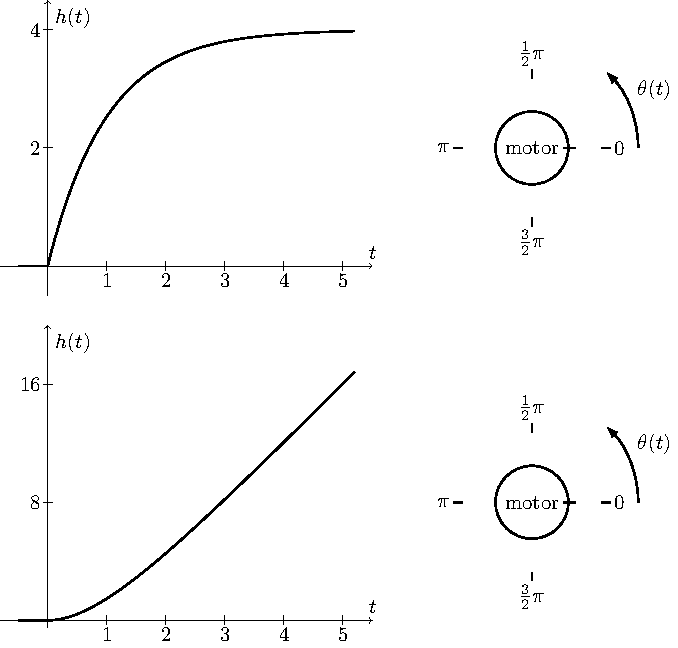
\includegraphics[page=1]{tikzfigs/dcmotorimpulseresponse}
\fi
  \caption{Impulse response (top) and step response (bottom) of a DC motor with constants $K_b= \tfrac{1}{4}$, $K_\tau = 8$ and $B=R=J=1$.} \label{fig:dcmotoranimimpulseresponse}
\end{figure}


% \section{Initial condition problems}

% The \term{unilateral Laplace transform}
% \[
% \calL_u(x,s) = \int_{0}^{\infty} x(t) e^{-st} dt
% \]



% \section{Feedback and control}\label{sec:control}

% Imagine that we would like to use a DC motor to drive an elevator that moves people between floors of a building.  Say that to move the elevator up a single floor the motor must make a single revolution, i.e., must increase it's angle by $2\pi$ radians.  As in Section~\ref{sec:direct-curr-motors-1} the equation describing the relationship between the input voltage signal and the angle of the motor is
% \[
% v = a D(\theta) + b D^2(\theta),
% \]
% where $a = \tfrac{RB}{K_\tau} + K_b$ and $b=\tfrac{RJ}{K_\tau}$ where $R,B,K_\tau,K_b,$ and $J$ and are related to components of the motor as described in Section~\ref{sec:direct-curr-motors}.

% Assume for the moment that the motor parameters satisfy $a=2$ and $b=3$.  Using the differential equation, we can design an input voltage signal that will make the motor perform a single revolution by $2\pi$, i.e., move the elevator up by one floor.  For example, put
% \begin{equation}\label{eq:thetaelevatordesigned}
% \theta(t) = \begin{cases}
% 0 & t \leq 0 \\
% \pi - \pi\cos(t) & 0 < t \leq \pi \\
% 2\pi & t > \pi.
% \end{cases}
% \end{equation}
% The input voltage signal corresponding with this signal $\theta$ is
% \begin{equation}\label{eq:velevatordesigned}
% v = 2 D(\theta) + 3 D^2(\theta) = \begin{cases}
% 0 & t \leq 0 \\
% 2\pi\sin(t) + 3\pi\cos(t)& 0 < t \leq \pi \\
% 0 & t > \pi.
% \end{cases}
% \end{equation}
% These signals are plotted in Figure~\ref{fig:designedelevatoropenloop}.  This input voltage signal drives the motor to perform precisely a rotation by $2\pi$, corresponding with the elevator moving up by a single floor.  

% This signal $v$ has been designed specifically for the case when $a = 2$ and $b=3$.  Say that the elevator is expected to carry up to a maximum of 6 people.  The inertial load $J$ on the motor varies with the number of passengers.  Also, it is found that during periods of consistent use the motor heats up causing the internal resistance of the motor $R$ to change.  After these effects are taken into account it is found that the coefficients $a$ and $b$ in the differential equation describing the motor can vary within the ranges $1 \leq a \leq 3$ and $1 \leq b \leq 7$.  These changes affect our ability to control the elevator.  From~\eqref{eq:impulseresponseDCmotor}, the impulse response of the motor is
% \[
% h(t) =  \tfrac{1}{a} u(t)\big( 1 - e^{-a t/b}\big).
% \]
% For any given $a$ and $b$ the reponse of the motor to input voltage $v$ from~\eqref{eq:velevatordesigned} is 
% \[
% \theta_{a,b}(t) =  h * v = \int_{-\infty}^{\infty} h(\tau) v(t - \tau) d\tau,
% \]
% and this can be shown (Exercise~\eqref{exer:elevatorgeneralequation}) to take the from
% \begin{equation}\label{eq:generalequationelevator}
% \theta_{a,b}(t) = \begin{cases}
% 0 & t \leq 0 \\
% \frac{2\pi}{a} + A e^{-at/b} +  B\cos(t) +  C \sin(t) & 0 < t \leq \pi\\
% \frac{4\pi}{a} +  A e^{-at/b} (1+e^{a\pi/b}) & t > \pi,
% \end{cases}
% \end{equation}
% where 
% \[
% A = \frac{\pi(3a - 2b)b}{a(a^2+b^2)}, \qquad  B =  -\frac{\pi(2a +3b)}{a^2+b^2}, \qquad C = \frac{a}{b}A.
% \]

% Figure~\ref{eq:motorelevatoropenloop} plots the motor angle signal $\theta_{a,b}$ for pairs $(a,b) = (2,3)$, $(4,3)$, $(2,1)$, $(2,7)$, $(1.5,3)$, $(3,3)$.

% \begin{figure}[tp]
%   \centering
%   \defaultanimation{tikzfigs/designedperfectopenloopmotor}  
%   \animategraphics[autoplay,loop,every=\every]{\defaultframerate}{tikzfigs/designedperfectopenloopmotor}{}{}
%   \caption{Motion of DC motor with input voltage~\eqref{eq:velevatordesigned} when $a=2$ and $b=3$.}\label{fig:designedelevatoropenloop}
% \end{figure}

% \begin{figure}[p]
%   \centering
%   \defaultanimation{tikzfigs/openloopdcmotors}  
%   \animategraphics[autoplay,loop,every=\every]{\defaultframerate}{tikzfigs/openloopdcmotors}{}{}
%   \caption{Motion of DC motor with input voltage~\eqref{eq:velevatordesigned} for cofficient pairs $(a,b) = (2,3)$, $(4,3)$, $(2,1)$, $(2,7)$, $(1.5,3)$, $(3,3)$.}\label{eq:motorelevatoropenloop}
% \end{figure}


% %The DC motor is not stable.  Let $H$ be the system that maps input voltage $x$ to motor angle $y$.  Assume we are able to measure the angle of the motor $\theta$.  Consider the system that results from applying a system $G$ to $\theta$ and adding this to the input voltage signal $x$ before it is input to the motor.  This is depicted in Figure~\ref{blockdiag:feedback}.  The input voltage and motor angle now satisfy

% Let $H$ be a linear time invariant system.  Assume that the signal $y$ output from $H$ can be measured.  Consider the system that results from applying a system $G$ to $y$ and adding the resopnse to an input signal $x$, that is then input to the system $H$.  This is depicted in Figure~\ref{blockdiag:feedback}. 
% \[
% y = H\big( x + G(y) \big) = H(x) + H\big(G(y)\big).
% \]
% Taking Laplace tranforms on both sides
% \[
% \calL(y) = \lambda(H)\calL(x) + \lambda(H)\lambda(G)\calL(y)
% \]
% and we find a system that maps $x$ to $y$, say $F$, now has transfer function
% \[
% \lambda(F) = \frac{\calL(y)}{\calL(x)} = \frac{\lambda(H)}{1 - \lambda(H)\lambda(G)}.
% \]
% The system $H$ might not have desirable properties, but if $G$ is appropriately chosen, the system $F$ might have more desirable properties.




% \begin{figure}
%   \centering
%   \begin{tikzpicture}[node distance=1.5cm,auto,>=latex']

%     \node [dspnodeopen] (x) [label=left:$x$] {};
%     \node[dspadder] (adder) [right of=x] {};
%     \node[coordinate] (belowadder) [below of=adder] {};
%     \node [dspsquare] (H) [right of=adder] {$H$};    
%     \node[coordinate] (feedbackconnector) [right of=H] {};
%     \node[coordinate] (belowfeedbackconnector) [below of=feedbackconnector] {};
%     \node [dspnodeopen] (y) [right of=feedbackconnector,label=right:$y$] {};
%     \node [dspsquare] (G) [below of=H] {$G$}; 

%     \draw[dspflow] (x) -- (adder);
%     \draw[dspflow] (adder) -- (H);
%     \draw[dspflow] (H) -- (feedbackconnector);
%     \draw[dspflow] (feedbackconnector) -- (y);
%     \draw[dspflow] (feedbackconnector) -- (belowfeedbackconnector);
%     \draw[thick,line cap=round] (belowfeedbackconnector) -- (G);
%     \draw[thick,line cap=round] (G) -- (belowadder);
%     \draw[dspflow] (belowadder) -- (adder);

%     \node (F) at (3,-0.75) [draw,thick,dashed,minimum width=3.9cm,minimum height=3cm,label=above:$F$] {};

%   \end{tikzpicture}
%   \caption{Feedback block diagram.  The system $F$ satisfies $y = H\big(x + G(y)\big)$.}\label{blockdiag:feedback}
% \end{figure}


\section{Exercises}

\begin{excersizelist}

\item Sketch the signal
\[
x(t) = e^{-2t} u(t) + e^{t} u(-t)
\]
where $u(t)$ is the step function.  Find the Laplace transform of $x(t)$ and the corresponding region of convergence (ROC).  Sketch the region of convergence on the complex plane.
\begin{solution}
\begin{center}
\begin{tikzpicture}[samples=200]
    %\draw[very thin,color=gray] (-0.1,-1.1) grid (3.9,3.9);
    \draw[->] (-5.1,0) -- (5.1,0) node[above] {$t$};
    \draw[->] (0,-0.3) -- (0,2.3) node[left] {$e^{-2t} u(t) + e^{t} u(-t)$};
    %\draw[color=black] plot[id=x] function{1/x^2} 
    %    node[right] {$f(t) = t^{-2}$};
    \draw[smooth,color=black,domain=-5:0,thick] plot function{2*exp(x)};
    \draw[smooth,color=black,domain=0:5,thick] plot function{2*exp(-2*x)};
    %\draw[color=black] plot[id=exp] function{0.05*exp(x)} 
    %    node[right] {$f(t) = \frac{1}{20} e^t$};
\end{tikzpicture}
\end{center}

The Laplace transform of $e^{-2t}u(t)$ is
\begin{align*}
\calL(e^{-2t}u(t), s) &= \int_{-\infty}^{\infty} e^{-2t}u(t) e^{-st} dt \\
&= \int_{0}^{\infty} e^{-(s+2)t} dt \\
&= -\frac{e^{-(s+2)t}}{s+2} \vert_{0}^\infty \\
&= \frac{1}{s+2}, \qquad \Re(s) > -2
\end{align*}
and the Laplace transform of $e^{t}u(-t)$ is
\begin{align*}
\calL(e^{t}u(-t), s) &= \int_{-\infty}^{0} e^{-(s-1)t} dt \\
&= -\frac{e^{-(s-1)t}}{s-1} \vert_{-\infty}^0 \\
&= -\frac{1}{s-1}, \qquad \Re(s) < 1.
\end{align*}
Thus, the Laplace transform of $e^{-2t} u(t) + e^{t} u(-t)$ is
\[
\calL(e^{-2t} u(t) + e^{t} u(-t), s) = \frac{1}{s+2} - \frac{1}{s-1}, \qquad -2 < \Re(s) < 1
\]
and the region of convergence (ROC) is the subset of the complex plane satisfying $-2 < \Re(s) < 1$.  The unshaded region in the plot below depicts the ROC.

\begin{center}
\begin{tikzpicture}
  \path [draw=none,fill=lightgray] (-2.5,-2.5)--(-1,-2.5)--(-1,2.5)--(-2.5,2.5)--cycle;
  \path [draw=none,fill=lightgray] (2.5,2.5)--(0.5,2.5)--(0.5,-2.5)--(2.5,-2.5)--cycle;
  \vtick{-1} node[pos=0.5,below] {$-2$};
  \vtick{0.5} node[pos=0.5,below] {$1$};
  \draw [<->] (-2.5,0) -- (2.5,0) node [right]  {$\Re$};
  \draw [<->] (0,-2.5) -- (0,2.5) node [above] {$\Im$};
\end{tikzpicture}
\end{center}
\end{solution}

\item \label{excer:laplacetransformcommonpolyut} Find the Laplace transform of the signal $t^n u(t)$ where $n\geq 0$ is an integer.
\begin{solution}
We have
\[
\calL\big(t^nu(t)\big) = \int_{-\infty}^{\infty} t^nu(t) e^{-st} dt = \int_{0}^{\infty} t^n e^{-st} dt.
\]
Integration by parts gives the indefinite integral
\[
\int t^n e^{-st} dt = \frac{t^n}{s} e^{-st} + \frac{n}{s} \int t^{n-1} e^{-st} dt.
\]
So, when $\Re(s) > 0$,
\begin{align*}
\calL\big(t^nu(t)\big) &= \lim_{t \to 0}\frac{t^n}{s} e^{-st} - \lim_{t \to \infty}\frac{t^n}{s} e^{-st} + \frac{n}{s} \int_{0}^\infty t^{n-1} e^{-st} dt \\
&= \frac{n}{s} \calL\big(t^{n-1}u(t)\big),
\end{align*}
since both limits converge to zero.  Unravelling the above recursive equation gives
\[
\calL\big(t^nu(t)\big) = \frac{n}{s}\times\frac{n-1}{s}\times\cdots\times\frac{1}{s}\times\calL\big(u(t)\big) = \frac{n!}{s^{n+1}}, \qquad \Re(s) > 0,
\]
since $\calL\big(u(t)\big) = \tfrac{1}{s}$ when $\Re(s) >0$. 
\end{solution}

\item Let $n \geq 0$ be an integer.  Show that the Laplace transform of the signal $- t^n u(-t)$ is the same as the Laplace transform of the signal $t^n u(t)$, but with a different region of convergence.
\begin{solution}
We have
\begin{align*}
\calL\big(-t^nu(-t)\big) &= -\int_{-\infty}^{\infty} t^nu(-t) e^{-st} dt \\
&= \int_{-\infty}^{\infty} (-t)^{n+1} u(t) e^{st} dt \qquad \text{(change variable t = -t)} \\
&= (-1)^{n+1} \int_{-\infty}^{\infty} t^n u(t) e^{st} dt \\
&= (-1)^{n+1} \calL( t^n u(t), -s) \qquad \Re(s) < 0 \\
&= (-1)^{n+1} \frac{n!}{(-s)^{n+1}} \qquad \Re(s) < 0 \\
&= \frac{n!}{s^{n+1}} \qquad \Re(s) < 0.
\end{align*}
\end{solution}


\item \label{exer:laplacetransdiffandtimeshift} Show that equation~\eqref{eq:transferLaplcetheorem} on page~\pageref{eq:transferLaplcetheorem} holds when the system $H$ is the differentiator $D^k$ or the time shifter $T_\tau$. 
\begin{solution}
Put $y = T_\tau(x) = x(t- \tau)$.  Taking Laplace transforms
\begin{align*}
\calL(y) &= \calL\big(T_\tau(x)\big) \\
&= \int_{-\infty}^{\infty} T_\tau(x,t) e^{-st} dt \\
&= \int_{-\infty}^{\infty} x(t - \tau) e^{-st} dt \\
&= \int_{-\infty}^{\infty} x(\kappa) e^{-s(\kappa + \tau)} d\kappa \qquad \text{(ch. vars. $\kappa = t - \tau$)} \\
&= e^{-s\tau}\int_{-\infty}^{\infty} x(\kappa) e^{-s\kappa} d\kappa \\
&= e^{-s\tau} \calL(x) \qquad s \in R_x \\
&= \lambda(T_\tau) \calL(x) \qquad s \in R_x
\end{align*}
as required.  Observe that the region of convergence of the time shifted signal $T_\tau(x)$ is the same as that of $x$.

% We now show the result for the differentiator $D$.  The argument we use is based on that of \citet[page~179]{Rudin_real_and_complex_analysis}.  We have just shown that the Laplace transform of the time shifted $T_{-\tau}(x,t) = x(t + \tau)$ is $e^{\tau s}\calL(x,s)$ with region of convergence $R_x$.  Since the Laplace transform is linear
% \[
% \calL\left( \frac{T_{-\tau}(x) - x}{\tau} \right) =  \frac{e^{\tau s} - 1}{\tau}\calL(x).
% \]
% We now consider what happens to both sides of this equation as $\tau \to 0$.  Application of L'Hopitals rule shows that
% \[
% \lim_{\tau \to 0}\frac{e^{\tau s} - 1}{\tau} = s,
% \]
% and so, the right hand side satisfies
% \[
% \lim_{\tau \to 0} \frac{e^{\tau s} - 1}{\tau}\calL(x) = s \calL(x).
% \]
% On the left hand side we have
% \[
% \lim_{\tau \to 0} \calL\left( \frac{T_{-\tau}(x) - x}{\tau} \right) = \lim_{\tau \to 0} \int_{-\infty}^\infty  \frac{x(t+\tau) - x(t)}{\tau} e^{-st} dt.
% \]
% Observe that
% \[
% \lim_{\tau \to 0} \frac{x(t+\tau) - x(t)}{\tau} = D(x)
% \]
% by definition of the differentiator $D$.  Lebesgue's dominated convergence theorem~\cite[page~26]{Rudin_real_and_complex_analysis} can be used to justify exchanging limits and integration so that
% \begin{align*}
%  \lim_{\tau \to 0} \int_{-\infty}^\infty  \frac{x(t+\tau) - x(t)}{\tau} e^{-st} dt &=  \int_{-\infty}^\infty  \lim_{\tau \to 0} \frac{x(t+\tau) - x(t)}{\tau} e^{-st} dt \\
% &= \int_{-\infty}^\infty D(x,t) e^{-st} dt = \calL\big(D(x)\big).
% \end{align*}
% We now have  $\calL\big(D(x)\big) = s\calL(x) = \lambda(D) \calL(x)$ as required.

We now show the result for the differentiator $D$.  Our approach works for all functions that will be of interest to us.  An alternative approach makes use of Lebesque's dominated convergence theorem~\citep[page~179]{Rudin_real_and_complex_analysis}.  
Put $y = D(x)$.  Taking Laplace transforms
\[
\calL(y) = \calL\big(D(x)\big) = \int_{-\infty}^{\infty} D(x,t) e^{-st} dt.
\]
Integrating by parts 
\[
\calL(y) = \big[ x(t) e^{-st} \big]_{-\infty}^\infty + s\int_{-\infty}^{\infty} x(t) e^{-st} dt = \big[ x(t) e^{-st} \big]_{-\infty}^\infty + s\calL(x).
\]
The assumption that we make is that 
\[
\lim_{t\to\infty} x(t) e^{-st} = 0 \qquad \text{and} \qquad \lim_{t\to-\infty} x(t) e^{-st} = 0
\]
whenever $s$ is in the region of convergence of both $x$ and $y$.  In this case $\calL(y) = s\calL(x)$ as required.  Observe that our assumption is true if, for example, $x(t)$ is finite.

The result follows for the $k$th differentiator $D^k$ because
\[
\calL\big( D^k(y) \big) = \calL\big( D(D^{k-1}(y)) \big) = s \calL\big( D^{k-1}(y) \big)
\]
and unravelling this recursion gives
\[
\calL\big( D^k(y) \big) = \underbrace{s \times s \times \dots \times s}_{\text{$k-1$ times}} \times \calL\big( D(y) \big) = s^k \calL( y ) = \lambda(D^k)\calL(y) 
\]
as required.
\end{solution}


\item What is the transfer function of the integrator system $I_\infty$ and what is its region of convergence? 
\begin{solution}
We have
\[
I_\infty(e^{st}) = \int_{-\infty}^t e^{s\tau} d\tau = \frac{e^{st}}{s} - \lim_{t\to -\infty}\frac{e^{st}}{s}
\]
and the limit exists only when $\Re{s} > 0$ and in this case it is zero.  So
\[
I_\infty(e^{st}) = \frac{1}{s} e^{st} \qquad \Re{s} > 0
\]
and $\lambda(I_\infty) = \tfrac{1}{s}$.
\end{solution}


\item \label{exer:partialfracfirstorder} By partial fractions, or otherwise, assert that
\[
\frac{as}{s+b} = a - \frac{ab}{s+b}
\]
\begin{solution}
Adding and subtracting $ab$ from the numerator
\[
\frac{as+ab-ab}{s+b} = \frac{a(s+b)-ab}{s+b} = \frac{a(s+b)}{s+b} - \frac{ab}{s+b} = a - \frac{ab}{s+b}
\]
\end{solution}

\item \label{exer:partialfracsecondorder} By partial fractions, or otherwise, assert that
\[
\frac{s + c}{(s+a)(s+b)} = \frac{a-c}{(a-b)(s+a)} + \frac{c-b}{(a-b)(s+b)}
\]
\begin{solution}
Hypothesise the solution
\[
\frac{s + c}{(s+a)(s+b)} = \frac{A}{s+a} + \frac{B}{s+b}.
\]
Multiplying both sides by $(s+a)(s+b)$,
\[
s+c = A(s+b) + B(s+a).
\]
Putting $s = -a$ gives $c-a = A(b-a)$, and pitting $s=-b$ gives $c-b = B(a-b)$, and so,
\[
\frac{s+c}{(s+a)(s+b)} = \frac{a-c}{(a-b)(s+a)} + \frac{c-b}{(a-b)(s+b)}.
\]
\end{solution}

\item \label{exer:partialfracfourthorder} By partial fractions, or otherwise, assert that
\[
\frac{1}{s(s-a)(s-b)(s-b^*)} = \frac{A_0}{s} + \frac{A_1}{s-a} + \frac{A_2}{s-b} + \frac{A_2^*}{s-b^*}
\]
where $a \in \reals$ and $b \in \complex$ and $\Im(b) \neq 0$ and
\[
A_0 = -\frac{1}{a\sabs{b}^2}, \qquad A_1 =  \frac{1}{a\sabs{a - b}^2}, \qquad A_2 = \frac{1}{b(b-a)(b-b^*)}.
\]
You might wish to check your solution using a symbolic programming language (for example Sage, Mathematica, or Maple).
\begin{solution}
The mathemtica command
\begin{verbatim}
Apart[1/s/(s - a)/(s - b)/(s - c), s]
\end{verbatim}
returns the equation
\[
\frac{1}{s(s-a)(s-b)(s-c)} = \frac{A_0}{s} + \frac{A_1}{s-a} + \frac{A_2}{s-b} + \frac{A_3}{s-b^*} -\frac{1}{a b c s}+\frac{1}{}+\frac{1}{}+\frac{1}{ (s-c)}
\]
where
\[
A_0 = -\frac{1}{abc}, \qquad A_1 =  \frac{1}{a (a-b) (a-c)}, 
\]
\[
A_2 = \frac{1}{b (b-a) (b-c)}, \qquad A_3 = \frac{1}{c (c-a) (c-b)}.
\]
Setting $c = b^*$ gives
\[
A_0 = -\frac{1}{a\sabs{b}^2}, \qquad A_1 =  \frac{1}{a\sabs{a - b}^2}, 
\]
\[ 
A_2 = \frac{1}{b(b-a)(b-b^*)}, \qquad A_3 = \frac{1}{b^*(b^*-a)(b^*-b)} = A_2^*
\]
as required.
\end{solution}


\item Let
\[
\calL(y) = \frac{2s + 1}{s^2 + s - 2}
\]
be the Laplace transform of a signal $y$.  By partial fractions, or otherwise, find all possible signals $y$ and their regions of convergence. 
\begin{solution}
Factorise the polynomial on the denominator
\[
\frac{2s + 1}{(s+2)(s-1)}.
\]
Adding and subtracting $s-1$ on the numerator 
\begin{align*}
\frac{2s + 1 + (s-1) - (s-1)}{(s+2)(s-1)} &= \frac{s-1}{(s-1)(s+2)} + \frac{s+2}{(s-1)(s+2)} \\
&= \frac{1}{s+2} + \frac{1}{s-1}.
\end{align*}
There are two time domain signals with Laplace transform $\frac{1}{s+2}$,
\[
e^{-2t} u(t), \; \Re(s) > -2 \qquad \text{and} \qquad -e^{-2t}u(-t), \; \Re(s) < -2,
\] 
and two time domain signals with Laplace transform $-\frac{1}{s-1}$,
 \[
e^{t}u(t), \; \Re(s) > 1 \qquad \text{and} \qquad -e^{t} u(-t), \; \Re(s) < 1.
\] 
There are three possible signals with nonempty regions of convergence
\[
y(t) = e^{-2t} u(t) - e^{t} u(-t) \qquad -2 < \Re(s) < 1,
\]
\[
y(t) = e^{-2t} u(t) + e^{t} u(t) \qquad 1 < \Re(s),
\]
\[
y(t) = - e^{-2t} u(-t) - e^{t} u(-t) \qquad \Re(s) < -2.
\]
\end{solution}

\item \label{excer:timescalelaplace} Let $x$ be a signal with region of convergence $R$.  Show that the time scaled signal $x(\alpha t)$ with $\alpha \neq 0$ satisfies equation~\eqref{eq:timescalingpropertrylaplacetrans} on page~\pageref{eq:timescalingpropertrylaplacetrans}.
\begin{solution}
First consider when $\alpha = -1$ so that $x(-t)$ is the reflection of the signal $x$ in time (see Section~\ref{sec:some-import-syst}).  We have 
\begin{align*}
 \calL\big( x(-t), s \big) &=  \int_{-\infty}^{\infty} x(-t)  e^{-s t} dt \\
 &=  -\int_{\infty}^{-\infty} x(\tau)  e^{s\tau} d\tau & \text{(change variable $\tau = -t$)}\\
 &=  \int_{-\infty}^{\infty} x(\tau)  e^{ s \tau} d\tau = \calL(x, -s) \qquad \Re(-s) \in R.
 \end{align*}
 This special case is called the \term{time reversal property}.  Now, when $\alpha > 0$,
 \begin{align*}
 \calL\big( x(\alpha t), s \big) &=  \int_{-\infty}^{\infty} x(\alpha t)  e^{-s t} dt \\
 &=  \frac{1}{\alpha} \int_{\infty}^{\infty} x(\tau)  e^{-s \tau / \alpha}  d\tau & \text{(change variable $\tau = \alpha t$)}\\
 &= \frac{1}{\alpha} \calL(x, s / \alpha) \qquad \Re(s/\alpha) \in R.
 \end{align*}
Combining this with the time reversal property we obtain
 \[
 \calL\big(x(\alpha t),s\big) = \frac{1}{\abs{\alpha}} \calL(x, s/\alpha), \qquad a \neq 0, \Re(s/\alpha) \in R.
 \]
as required.
\end{solution}

% \item \label{exer:thetainfinitelydiff} Plot the signal $\theta(t)$ from~\eqref{eq:thetainfinitediff} and its first 2 derivatives $D(\theta)$ and $D^2(\theta)$. Show that this signal is infinitely differentiable, that is, that it can be differentiated as many times as you like.
% \begin{solution}

% \end{solution}

% \item \label{exer:elevatorgeneralequation} Show that the response of the DC motor to input voltage $v$ from~\eqref{eq:velevatordesigned} satisfies~\eqref{eq:generalequationelevator}.  That is, show that convolution of the impulse response of the motor $h(t) = \tfrac{1}{a} u(t)\big( 1 - e^{-a t/b}\big)$ and the voltage signal $v$ is given by~\eqref{eq:generalequationelevator}.  You may wish to use a symbol programming language (for example Sage, Mathematica, or Maple).
% \begin{solution}
% The following Mathematica commands immediately yield this solution
% \begin{verbatim}
% Theta[t_] := (UnitStep[t] - UnitStep[t - Pi])*Pi*(1-Cos[t]) + 2*Pi*UnitStep[t - Pi];
% v[t_] := 2*Theta'[t] + 3*Theta''[t];
% h[t_, a_, b_] := UnitStep[t]*(1 - Exp[-a/b*t])/a;
% FullSimplify[
% Integrate[
%   h[Tau, a, b]*v[t - Tau], {Tau,-Infinity,Infinity}, 
%   Assumptions -> t Element Reals]]
% \end{verbatim}
% \end{solution}

\item Consider the active electrical circuit from Figure~\ref{elec:activeRC} described by the differential equation from~\eqref{eq:twoaparrarrelRCactive}.  Derive the transfer function of this system.  Find an explicit system $H$ that maps the input voltage $x$ to the output voltage $y$.  State whether this system is stable and/or regular.
\begin{solution}
The differential equation modelling the circuit is
\[
-\frac{x}{R_1} - C_1 D(x) = \frac{y}{R_2} + C_2 D(y),
\]
and taking Laplace transforms on both sides of this equation
\[
\calL{y} = -\frac{\tfrac{1}{R_1} + C_1s}{\tfrac{1}{R_2} + C_2s} \calL(x) = -\frac{\alpha + \gamma s}{\beta + s}
\]
where $\alpha = \tfrac{1}{R_1C_2}$, $\beta = \tfrac{1}{R_2C_2}$, and $\gamma = \tfrac{C_1}{C_2}$.  The transfer function of the system mapping $x$ to $y$ is correspondingly
\[
\lambda(H) = -\frac{\alpha + \gamma s}{\beta + s} = -\frac{\alpha}{\beta + s} - \frac{\gamma s}{\beta + s}
\]
Applying partial fraction (as in Exercise~\ref{exer:partialfracfirstorder}) to the second term gives
\[
\lambda(H) = -\frac{\alpha + \gamma\beta}{\beta + s} - \gamma
\]
The first term $-\frac{\alpha + \gamma\beta}{\beta + s}$ corresponds with a regular system, say $H_2$, having impulse response
\[
h_2 = -(\alpha + \gamma\beta) u(t) e^{-\beta t}
\]
by using the Laplace transform pair from~\eqref{eq:laplacetneucommon} with the integer $n=0$.  The term $-\gamma$ correspond with the system $H_1 = \gamma T_0$, i.e, the identity system multiplied by $-\gamma$.  The system $H$ that describes the mapping between input voltage $x$ and output voltage $y$ is thus
\[
H(x) = H_1(x) + H_2(x) = -\gamma x + h_2 * x.
\]
The system is not regular because the $H_1$ is not regular.  The system is stable because $H_1$ is stable and $H_2$ is stable because the impulse response $h_2$ is absolutely integrable since $\beta = \tfrac{1}{R_2C_2} > 0$.  Equivalently the system is not regular because the transfer function does not have more poles than zero, and the system is stable because the transfer function has at least as many poles as zeros (equal in this case), and because all the poles lie strictly in the left half plane. 
\end{solution}

\item \label{exer:massspringdamperrect} Given the mass spring damper system described by~\eqref{eq:masspringeqseclapltrans}, find the position signal $p$ given that the force signal 
\[
f(t) = \rect\big(t-\tfrac{1}{2}\big) = \begin{cases}
1 & 0 < t \leq 1 \\
0 & \text{otherwise}
\end{cases}
\]
is the rectangular function time shifted by $\tfrac{1}{2}$.  Consider three cases:
\begin{enumerate}
\item $M=1$, $K=\tfrac{\pi^2}{4}$ and $B=\tfrac{\pi}{3}$,
\item $M=1$, $K=\tfrac{\pi^2}{4}$ and $B=\pi$,
\item $M=1$, $K=\tfrac{\pi^2}{4}$ and $B=2\pi$,
\end{enumerate}
Plot the solution in each case, and comment on whether the system is underdamped, overdamped, or critically damped. 
\begin{solution}
Observe that the input force signal can be written as the sum of the step function $u$ and its negated time-shift, that is,
\[
f(t) = u(t) - u(t - 1) = u(t) - T_{1}(u,t)
\]
and so, the response of the linear, time invariant system $H$ modelling the mass spring damper to input force signal $f$ is
\[
H(f) = H\big(u - T_{1}(u)\big) = H(u) - T_{1}\big(H(u)\big),
\]
and so, $H(f,t) = H(u,t) - H(u,t-1)$, where $H(u)$ is the step response of the system.  The step responses are described in Section~\ref{sec:second-order-systems}.  As described in Section~\ref{sec:second-order-systems}, the system is underdamped when $B = \tfrac{\pi}{3}$, critically damped when $B = \pi$ and overdamped when $B = 2\pi$.
\end{solution}

\item Plot the signal $x(t) = \sin(t e^t) u(t)$ and find and plot its derivative $D(x)$.  Show that the region of convergence of $x$ contains those complex numbers $s$ with $\Re(s) > 0$ and that the region of convergence of $D(x)$ contains those with $\Re(s) > 1$.
\begin{solution}
By application of the chain rule the derivative of $\sin(t e^t)$ is $(t+1)e^t \cos(e^t) u(t)$.  These signals are plotted below.
\begin{center}
\begin{tikzpicture}
\begin{scope}[xscale=1.5]
    \draw[->] (-0.5,0) -- (2.8,0) node[above] {$t$};
    \draw[->] (0,-1.3) -- (0,1.3) node[above right] {$\sin(t e^t) u(t)$};
    \draw[thick] (-0.25,0) -- (0,0);
    \draw[smooth,color=black,domain=0:2.5,thick,samples=300] plot function{sin(x*exp(x))};
\end{scope}
\htick{1} node[pos=0.5,left] {$1$};
\htick{-1} node[pos=0.5,left] {$-1$};
\end{tikzpicture}
\end{center}
\begin{center}
\begin{tikzpicture}
\begin{scope}[xscale=1.5,yscale=0.05]
    \draw[->] (-0.5,0) -- (2.8,0) node[above] {$t$};
    \draw[->] (0,-40.3) -- (0,40.3) node[above right] {$(t+1)e^t \cos(t e^t) u(t)$};
    \draw[thick] (-0.25,0) -- (0,0);
    \draw[smooth,color=black,domain=0:2.5,thick,samples=300] plot function{(1+x)*exp(x)*cos(x*exp(x))};
    \draw[smooth,color=black,domain=0:2.45,thick,samples=50,dashed] plot function{(1+x)*exp(x)};
    \draw[smooth,color=black,domain=0:2.45,thick,samples=50,dashed] plot function{-(1+x)*exp(x)};
\end{scope}
\begin{scope}[yscale=0.05]
\htick{30} node[pos=0.5,left] {$30$};
\htick{-30} node[pos=0.5,left] {$-30$};
\end{scope}
\end{tikzpicture}
\end{center}

We have $\abs{x(t)} = \abs{\sin(t e^t) u(t)} < 1$ for all $t \in \reals$ and so
\begin{align*}
\calL\big( x , s\big) &= \int_{-\infty}^\infty \sin(t e^t) u(t) e^{-s t} dt \\
&= \int_{0}^\infty \sin(t e^t) e^{-s t}  dt \\
&\leq = \int_{0}^\infty \abs{\sin(t e^t) e^{-s t}}  dt \\
&\leq \int_{0}^\infty e^{-\Re(s) t}  dt
\end{align*}
which is finite for all $s$ with $\Re(s) > 0$ as required.  For the derivative we have
\begin{align*}
\calL\big( D(x) , s\big) &= \int_{-\infty}^\infty (t+1)e^t \cos(t e^t) u(t) e^{-s t} dt \\
&= \int_{0}^\infty (t+1) \cos(t e^t) e^{-(s-1) t}  dt \\
&\leq \int_{0}^\infty \abs{(t+1) \cos(t e^t) e^{-(s-1) t}}  dt \\
&\leq \int_{0}^\infty (t+1) e^{-(\Re(s)-1) t}  dt
\end{align*}
which is finite for all $s$ with $\Re(s) > 1$ as required.
\end{solution}


\end{excersizelist}



%\clearpage
\chapter{The Fourier transform}\label{sec:fourier-transform}
\newcommand{\calF}{{\mathcal F}}

%BLERG: THE NONADVANCE PARTS OF THIS SHOULD BE MUCH SHORTER.  JUST MOTIVATE FOURIER TRANSFORM AS LAPLACE TRANSFORM ON THE IMAGINARY AXIS AND GET STRAIGHT TO FILTER DESIGN.  ADVANCED SECTION CAN DO INVERSION THEOREM, PLANCHEREL THEOREM AND SQUARE INTEGRABLE SIGNALS.

%BLERG: In this section signals will be assumed to be asolutely integrable unless otherwise stated.
%BLERG: Equality of signals means mean square equality in this section, i.e. x=y means \|x-y\|_2 = 0.

The \term{Fourier transform} of an absolutely integrable signal $x$ is defined as
\begin{equation}\label{eq:fouriertransform}
\calF(x) = \int_{-\infty}^\infty x(t) e^{-j2\pi ft} dt.
\end{equation}
The Fourier transform is a function of the real number $f$. We indicate its value at $f$ by $\calF(x)(f)$ or $\calF(x,f)$. For example, the rectangular pulse $\rect(t)$ from~\eqref{eq:rectfuncdefn} is absolutely integrable and has Fourier transform
\begin{align}
\calF(\rect) &= \int_{-\infty}^\infty \rect(t) e^{-j2\pi ft} dt \nonumber \\
&= \int_{-1/2}^{1/2} e^{-j2\pi ft} dt \nonumber  \\
&= \frac{e^{j\pi f} - e^{-j\pi f}}{j 2 \pi f} = \frac{\sin(\pi f)}{\pi f} = \sinc(f). \label{eq:sincandrect}
\end{align}
The $\sinc$ function is plotted in Figure~\ref{fig:sincfunction1}.  %As we will see in Section~\ref{sec:square-integr-sign}, square integrable signals also have Fourier transforms.  

The Fourier transform is closely related to the Laplace transform because
\[
\calF(x,f) = \calL(x,j 2\pi f)
\]
for those signals $x$ with region of convergence containing the imaginary axis, that is, for absolutely integrable $x$.  The Fourier transform inherits the properties of the Laplace transform that were described in Section~\ref{sec:transf-funct-lapl}.  For example, if $H$ is a stable regular system with absolutely integrable impulse response $h$ having Fourier transform $\calF(h)$, then the spectrum of $H$ satisfies
\[
\Lambda(H, f) = \lambda(H,j2\pi f) = \calL(h,j2\pi f) = \calF(h,f),
\]
that is, the spectrum of a stable regular system is given by the Fourier transform of its impulse response.  
% The spectrum of the time-shifter and differentiator can be obtained by inspection.  From~\eqref{eq:timeshiftertransferfunction}, the spectrum of the time shifter $T_\tau$ satisfies
% \[
% \Lambda(T_\tau,f) = \lambda(T_\tau,j 2\pi f) = e^{-j2\pi f \tau}
% \]
% and, from~\eqref{eq:lambdadifferentiator}, the spectrum of the $k$th differentiator $D^k$ is
% \[
% \Lambda(D^k,f) = \lambda(D^k,j 2\pi f) = (j 2\pi f)^k.
% \]
 Like the Laplace transform, the Fourier transform obeys the \term{convolution theorem}~\eqref{eq:convtheoremlaplace}, that is,
 \begin{equation}\label{eq:convthmfouriertransform}
 \calF(x * y) = \calF(x)\calF(y)
 \end{equation}
when each of the signals $x$, $y$, and $x * y$ are absolutely integrable.  In words: the Fourier transform of a convolution of signals is given by the multiplication of the Fourier transforms of those signals.

It follows from~\eqref{eq:transferLaplcetheorem} that if $H$ is a regular system with spectrum $\Lambda(H)$ and if $x$ is a signal with Fourier transform $\calF(x)$, then the signal $y = H(x)$ has Fourier transform
\[
\calF(y) = \Lambda(H) \calF(x).
\]
This property also holds for the differentiator system $D$ and the time shifter system $T_\tau$ (Exercise~\ref{eq:transferLaplcetheorem}).  From~\eqref{eq:timeshiftertransferfunction} and~\eqref{eq:lambdadifferentiator} the spectrum of $T_\tau$ and the $k$th differentiator $D^k$ satisfy 
%BLERG, it doesn't hold for the differentiator system all the time, but for certain signals, like those of rapid decent it does
\[
\Lambda(T_\tau) = e^{-j2\pi f \tau}, \qquad \Lambda(D^k) = (j2\pi f)^k
\]
from which we obtain the \term{time shift property},
 \[
 \calF\big(T_\tau(x)\big) = \Lambda(T_\tau) \calF(x) = e^{-j2\pi f \tau} \calF(x),
\]
and the \term{differentiation property},
\[
 \calF\big(D^k(x)\big) = \Lambda(D^k) \calF(x) =  (j2\pi f)^k \calF(x),
\]
of the Fourier transform.  These results motivate assigning the following Fourier transforms to the delta ``function'' and its derivatives
\begin{equation}\label{eqftsofdeltas}
\calF(\delta) = 1, \qquad \calL(\delta^k) = (j2\pi f)^k.
\end{equation}
These conventions are common in the literature~\citep{Oppenheiim_sigs_sys_1996}.  

Similarly to the Laplace transform~\eqref{eq:freqshiftrule}, the Fourier transform obeys a \term{frequency shift rule} that relates the transform of a signal $x(t)$ to that of the signal $e^{2\pi j \gamma f t} x(t)$ where $\gamma \in \reals$.  From~\eqref{eq:freqshiftrule}, the frequency shift rule asserts that
\begin{align}
\calF\big( e^{2\pi j \gamma t} x(t), f\big) =  \calF(x, f - \gamma). \label{eq:freqshiftrulefourier}
\end{align}
Since $\cos( 2\pi \gamma t) = \tfrac{1}{2}e^{2\pi j \gamma t} + \tfrac{1}{2}e^{-2\pi j \gamma t}$ we also have
\begin{equation}\label{eq:modulationpropertyft}
\calF\big( \cos(2\pi \gamma t) x(t), f \big) =  \frac{1}{2}\calF(x, f - \gamma) + \frac{1}{2}\calF(x, f + \gamma).
\end{equation}
% and, similarly, since $\sin( 2\pi \gamma t) = \tfrac{1}{2j}e^{2\pi j \gamma t} - \tfrac{1}{2j}e^{-2\pi j \gamma t}$ we have
% \[
% \calF\big( \sin(2\pi \gamma t) x(t), f \big) =  \frac{1}{2j}\calF(x, f - \gamma) + \frac{1}{2j}\calF(x, f + \gamma)
% \]
This is sometimes called the \term{modulation property} of the Fourier transform~\cite[page~61]{Papoulis_signal_analysis_1977}.  This property is of particular importance in communications engineering~\citep{Proakis_digital_comms}.  % Combing the frequency shift rule with the convention $\calF(\delta) = 1$ motivates assigning the the following Fourier transform to $e^{2\pi j \gamma t}$
% \[
% \calF(e^{2\pi j \gamma t},f) = 
% \]
%  and the following

Like the Laplace transform~\eqref{eq:timescalingpropertrylaplacetrans}, the Fourier transform obeys a~\term{time scaling property}.  If $x$ is an absolutely integrable signal then the time scaled signal $x(\alpha t)$ with $\alpha \neq 0$ has Fourier transform
\begin{equation}\label{eq:timescalingpropertryfouriertrans}
\calF\big( x(\alpha t), f \big) = \frac{1}{\abs{\alpha}} \calF\big( x , f/\alpha \big).
\end{equation}

% The Fourier transform also obeys a reciprocal property
% \[
% \calF(x y) = \calF(x)*\calF(y),
% \]
% that is, the Fourier transform of the multiplication of two signals, is given by the convolution of those signals Fourier transforms.  This is called the \term{modulation theorem} and we discuss it further in Section~\ref{}.


% Applying the inverse Fourier transform to a signal $x$ gives
% \[
% \int_{-\infty}^\infty x(f) e^{j2\pi ft} df =  \calF(x,-t).
% \]
% This is called the \term{duality} property.  Specifically, if $x$ is a signal with Fourier transform $\hat{x} = \calF(x)$, then the Fourier transform of the signal $\hat{x}(t)$ is $x(-f)$. The duality property gives us a method for assigning a Foutier transform to signals for which the integral in~\eqref{} does not converge uniquely. BLERG....can do this anyway using the inverse formula...

\begin{figure}
\centering
\begin{tikzpicture}[domain=-5.2:5.2,samples=200]
    \begin{scope}[yscale=2]
      % \def\sinc(#1){ifthenelse(abs(#1)>0.0001,sin(3.1415926*#1 r)/(3.1415926*#1),1)} %step function
      \draw[->] (-5.5,0) -- (5.5,0) node[above] {$t$};
      \draw[->] (0,-0.4) -- (0,1.25);
      \draw[smooth,color=black,thick] plot function{sin(3.1415926*x)/(3.1415926*x)};
      \vtick{4} node[pos=0.5,below right] {$4$};
      \vtick{2} node[pos=0.5,below right] {$2$};
      %\vtick{1} node[pos=0.5,below] {$1$};
      %\vtick{-1} node[pos=0.5,below] {$-1$};
      \vtick{-2} node[pos=0.5,below left] {$-2$};
      \vtick{-4} node[pos=0.5,below left] {$-4$};
      \htick{1} node[pos=0.5,above right] {$1$};
      %\htick{-0.2} node[pos=0.5,right] {$-0.2$};
    \end{scope}
  \end{tikzpicture}
\caption{The \term{sinc function} $\sinc(t) = \frac{\sin(\pi t)}{\pi t}$.} \label{fig:sincfunction1}
\end{figure}


\section{The inverse transform and the Plancherel theorem}\label{sec:square-integr-sign}

Given a signal $x$ we will often denote its Fourier transform by $\hat{x} = \calF(x)$.  Observe that $\hat{x}$, like $x$, is a function that maps a real number to a complex number.  Thus, the Fourier transform $\hat{x}$ is a \term{signal} with independent variable representing \term{frequency}.  It is usual to call $x$ the \term{time domain} representation of the signal and $\hat{x}$ the \term{frequency domain} representation.  If $\hat{x}$ is absolutely integrable, then $x$ can be recovered using the \term{inverse Fourier transform}
\begin{equation}\label{eq:inversefouriertransform}
x(t) = \calF^{-1}(\hat{x}) =  \int_{-\infty}^\infty \hat{x}(f) e^{j2\pi ft} df.
\end{equation}
For example, let $\hat{x} = \calF(x) = \rect$ be the rectangular pulse.  By working analogous to that from~\eqref{eq:sincandrect},
\[
x(t) = \int_{-\infty}^\infty \rect(f) e^{j2\pi ft} df = \sinc(-t) = \sinc(t).
\]
%because $\sinc$ is an even function.  
We are lead to the conclusion that the Fourier transform of $\sinc$ is the rectangular pulse $\rect$.

The rectangular pulse $\rect$ is finite and absolutely integrable.  The $\sinc$ function is not absolutely integrable (Exercise~\ref{exer:sincnotabsint}). Because of this the integral equation that we have used to define the Fourier transform~\eqref{eq:fouriertransform} cannot be directly applied to the $\sinc$ function.  %The inverse transform provides a method for assigning Fourier transforms to signals even when the formula~\eqref{eq:fouriertransform} does not apply.  
Although $\sinc$ is not absolutely integrable, it is square integrable (Exercise~\ref{exer:sincnotabsint}).  It happens that all square integrable signals can be assigned a Fourier transform by interpreting the integral in~\eqref{eq:fouriertransform} as what is called its~\term{Cauchy principal value}.  That is, for $x$ a square integrable signal, we assign the Fourier transform
\[
\hat{x} = \calF(x) = \lim_{T \to \infty}  \int_{-T}^T x(t) e^{-j2\pi ft} dt.
\]
This Fourier transform $\hat{x}$ is itself a square integrable signal and the orignal time domain signal $x$ can be recovered almost everywhere by taking the Cauchy principal value of the integral in~\eqref{eq:inversefouriertransform}, that is,
\[
x = \calF^{-1}(\hat{x}) = \lim_{T \to \infty}  \int_{-T}^T \hat{x}(f) e^{j2\pi f t} df \qquad \text{a.e.}.
\]
Infact, the energy of $x$ and its Fourier transform $\hat{x}$ are the same, that is,
\begin{equation}\label{eq:parseval}
\|x\|_2^2 = \int_{-\infty}^{\infty} \abs{x(t)}^2 dt = \int_{-\infty}^{\infty} \abs{\hat{x}(f)}^2 dt = \|\hat{x}\|_2^2.
\end{equation}
These results are known as the \term{Plancherel theorem}~\cite[Th.~9.13]{Rudin_real_and_complex_analysis}.  The equality of energies in~\eqref{eq:parseval} is often called~\term{Parseval's identity}.  For our purposes it will suffice to remember only that the Fourier transform of the $\sinc$ function is the rectangular pulse $\rect$.
  
A result more general than~\eqref{eq:parseval} holds.  If $x$ and $y$ are square integrable signals with Fourier transforms  $\hat{x}$ and $\hat{y}$, then
\begin{equation} \label{eq:parsevalxy}
\int_{-\infty}^{\infty} x(t)y^*(t) dt = \int_{-\infty}^{\infty} \hat{x}(f)\hat{y}^*(f) dt
\end{equation}
where the superscript $^*$ denotes the complex cojugate.  One obtains~\eqref{eq:parseval} by putting $y = x$ in~\eqref{eq:parsevalxy}. This more general result often also goes by the name of Parseval's identity.

%One can show that properties of the Fourier transform, such as the differentiation property, and the convolution theorem apply to the sinc function just as they do to absolutely integrable signals (Exercise~\ref{}).

%We have derived many properties of the Fourier transform, for example the convolution theorem, under the assumption that the signals involved are absolutely integrable.  These properties can be shown to hold when the signals are only square integrable.  We will not attempt to show this here.
%Many properties of the Fourier transform, for example the convolution theorem, have been derived under the assumption the signals involved are absolutely integral.  In what follows we will often apply these properties with the $\sinc$ function  %All other signals that we will have use of are absolutely integrable, and have a Fourier transform defined by the integral equation~\eqref{eq:fouriertransform}.

% Let $x$ and $y$ be signals such that $xy$, the signal that results from the multiplication of $x$ and $y$, is absolutely integrable.  The Fourier transform of $xy$ is 
% \[
% \calF( xy ) = \int_{-\infty}^\infty x(t)y(t) e^{-j2\pi ft} df.
% \] 
% If it is also that case $\hat{x} = \calF(x)$ is absolutely integrable then $x(t) = \int_{-\infty}^\infty \hat{\gamma} e^{j2\pi \gamma t} d\gamma$, and so,
% \begin{align*}
% \calF( xy ) &= \int_{-\infty}^\infty \left(\int_{-\infty}^\infty \hat{\gamma} e^{j2\pi \gamma t} d\gamma \right) y(t) e^{-j2\pi ft} df \\
% &= \int_{-\infty}^\infty \left(\int_{-\infty}^\infty  \hat{\gamma} e^{j2\pi \gamma t}   y(t) e^{-j2\pi ft} d\gamma df \\
% &= \int_{-\infty}^\infty \left(\int_{-\infty}^\infty  \hat{\gamma} e^{j2\pi \gamma t}   y(t) e^{-j2\pi ft} d\gamma df \\
% \end{align*}

Let $x$ be a signal with Fourier transform
\[
\calF(x,f) = \int_{-\infty}^{\infty} x(\tau) e^{-j2\pi f \tau} d\tau.
\]
Evaluating the Fourier transform at $-t$ we find that
\begin{equation}\label{eq:dualityft}
\calF(x,-t) = \int_{-\infty}^{\infty} x(\tau) e^{j2\pi t \tau} d\tau = \calF^{-1}(x,t).
\end{equation}
This is the called the \term{duality} property of the Fourier transform.  In words, if $\hat{x}$ is the Fourier transform of $x$, then $x$ is the Fourier transform of $\hat{x}$ reflected in time.    %Another way to express duality is
% \[
% \calF( \hat{x} ) = \calF( \calF(x)) = \calF^2(x) = x(-t),
% \]
% that is, twice application of the Fourier transform to a signal $x$ results in $x$ reflected in time.

% %BLERG: You can only really apply $\calF$ is \hat{x} is absolutely integrable, otherwise need a.e. qualifier.
% Equivalently, if we define 
% \begin{equation}\label{eq:timereflectionsystemR}
% R(x,t) = x(-t)
% \end{equation}
% as the system that reflects its input signal, then
% \[
% \calF( \calF(x) ) = \calF^2(x) = R(x), 
% \]
% %BLERG: Again needs a.e. qualifier.
% where we use the notation $\calF^2$ to denote application of the Fourier transform twice.   Applying the Fourier transform three times to a signal $x$ we obtain
% \begin{equation}\label{eq:fouriertransform3times}
% \calF^3(x) = \calF\big(\calF\big(\calF(x)\big)\big) = R\big(\calF(x)\big) = \calF\big(R(x)\big).
% \end{equation}
% It follows that the Fourier transform commutes with the reflection system $R$.  This is called the \term{reflection} property of the Fourier transform.  Informally stated: a reflection in the time domain causes a corresponding reflection in the frequency domain.

% % The duality property and~\eqref{eqftsofdeltas} motivates assigning a Fourier transform to the constant signal $1$, that is,
% % \[
% % \calF(1) = R(\delta) = \delta,
% % \]
% % where we treat the delta function as if it were even, i.e., we assign it the property $\delta(t) = \delta(-t)$ so that $R(\delta) = \delta$.  Combining this with the frequency shift rule~\eqref{eq:freqshiftrulefourier} motivates assigning the following Fourier transform to the complex exponential signal $e^{j2\pi \gamma t}$,
% % \[
% % \calF(e^{j2\pi \gamma t}) = \delta(f - \gamma),
% % \]
% % and, similarly, motivates assigning the Fourier transforms 
% % \[
% % \calF\big( \cos(2\pi t) \big) = \calF(\tfrac{1}{2}e^{j2\pi \gamma t} + \tfrac{1}{2}e^{-j2\pi \gamma t}) = \tfrac{1}{2}\delta(f - \gamma) + \tfrac{1}{2}\delta(f + \gamma) 
% % \]
% % and
% % \[
% % \calF\big( \sin(2\pi t) \big) = \calF(\tfrac{1}{2j}e^{j2\pi \gamma t} - \tfrac{1}{2j}e^{-j2\pi \gamma t}) = \tfrac{1}{2j}\delta(f - \gamma) - \tfrac{1}{2j}\delta(f + \gamma) 
% % \]
% % to the signals $\sin(2\pi t)$ and $\cos(2\pi t)$.  These conventions are common in the literature~\citep{Oppenheiim_sigs_sys_1996}.

% % It is important to remember that $\delta$ is not a signal.  It is not a function. The signals $1$, $e^{2\pi j t}$, $\cos(2\pi t)$, and $\sin(2\pi t)$ are neither absolutely integrable nor square integrable and do not formally have Fourier transforms.  You cannot, for example, apply the integral equation~\eqref{eq:fouriertransform} to these signals and expect a meaningful result.  Nevertheless, these conventions often lead to valid results when applied with discretion.
% % Applying the Fourier transform four times we find that
% % \[
% % \calF^4(x) = R\big(R(x)\big) = x
% % \]
% % because applying the reflection $R$ twice is equivalent to the identity system, i.e., $R^2 = T_0$.  Thus, applying the Fourier transform four times to a signal results in the same signal.  Because
% % \[
% % \calF^4(x) = \calF\big(\calF^3(x)\big) = \calF^3\big(\calF(x)\big) = x
% % \]
% % we find that $\calF^3(x) = \calF^{-1}(x)$, that is, the inverse Fourier transform is equivalent to applying the Fourier transform three times.  From~\eqref{eq:fouriertransform3times} we also have that the inverse transform is equivalent to applying the Fourier transform followed by a relection or a relfection followed by the Fourier transform, that is, 
% % \[
% % \calF^{-1}(x) = R\big(\calF(x)\big) = \calF\big(R(x)\big).
% % \]

% Let $\hat{x} = \calF(x)$ and $\hat{y} = \calF(y)$ be the Fourier transforms of signals $x$ and $y$.  By duality
% \[
% \calF( \hat{x} ) = \calF^2(x) =  R(x), \qquad \calF( \hat{y} ) = \calF^2(y) =  R(y).
% \]
% Because the product $R(x)R(y) = R(xy)$ we have
% \[
% R(xy) = R(x)R(y) = \calF( \hat{x} )\calF( \hat{y} ) = \calF( \hat{x} * \hat{y} ),
% \]
% where the last inequality follows from the convolution theorem~\eqref{eq:convthmfouriertransform}.  Applying the Fourier transform to both sides and using the duality and reflection properties we obtain
% \[
% R\big(\calF(xy)\big) = R( \hat{x} * \hat{y} ).
% \]
% Applying the reflection system $R$ to both sides and using the fact that $R^2 = T_0$ is the identity system we obtain
% \[
% \calF(xy) = \hat{x} * \hat{y} = \calF(x) * \calF(y).
% \]
% Thus, the Fourier transform of a product of signals is the product of the Fourier transforms.  This is called the \term{multiplication theorem}.  The multiplication theorem often goes by the phrase: ``Multiplication in the time domain is convolution in the frequency domain''. 

% % Combing the multiplication property with the conventions $\calF(\deta) = 1$ and $\calF(\delta^k) = (j2\pi f)^k$ motives assigning the following Fourier transform to $e^{2\pi j \gamma t}$,
% % \[
% % \calF(e^{2\pi j \gamma t} * \delta(t)) = 
% % \]

% % We have already seen an example of duality with regards to the rectangular pulse $\rect$ and the $\sinc$ function, specifically 
% % \[
% % \calF(\rect) = \sinc, \qquad \calF(\sinc) = \rect. 
% % \]
% % The reflection in time does not appear in this case because both $\sinc$ and $\rect$ are \term{even} signals, that is $\sinc(t) = \sinc(-t)$ and $\rect(t) = \rect(-t)$.  

% % The duality property provides a convenient way to find the Fourier transform of signals for which directly computing the integral~\eqref{eq:fouriertransform} is tedious.  For example, the Fourier transform of the signal $e^{-\alpha\abs{t}}$ with $\alpha > 0$ is readily shown to be (Exercise~\ref{exer:fourtransealphaabs})
% % \[
% % \calF(e^{-\alpha\abs{t}}) = \frac{2\alpha}{\alpha^2 + 4\pi^2f^2}.
% % \]
% % Direct computation of the Fourier transform of the signal $\frac{2\alpha}{\alpha^2 + 4\pi^2t^2}$ is less trivial.  However, the duality property immediately gives
% % \[
% % \calF\left( \frac{2\alpha}{\alpha^2 + 4\pi^2(-t^2)} \right) = \calF\left( \frac{2\alpha}{\alpha^2 + 4\pi^2t^2} \right) = e^{-\alpha\abs{f}}.
% %\]

% \section{Parseval's identity}\label{sec:parsevals-identity}

% Let $x$ be a signal with Fourier transform $\hat{x} = \calF(x)$.  The Fourier transform of $x^*$, the complex conjugate of $x$, satisfies
% \begin{align}
% \calF(x^*,f) &= \int_{-\infty}^\infty x(t)^* e^{-j2\pi ft} dt \nonumber \\
% &= \int_{-\infty}^\infty \big( x(t) e^{j2\pi ft} \big)^* dt  \nonumber \\
% &= \left(\int_{-\infty}^\infty x(t) e^{j2\pi ft} dt \right)^* \nonumber \\
% &= \calF(x,-f)^* \nonumber \\
% &= \hat{x}(-f)^*. \label{eq:calFofcong}
% \end{align}
% It follows that if $x$ is a real valued signal so that $x = x^*$, then $\hat{x}(f) = \hat{x}(-f)^*$.  That is, the Fourier transform of a real valued signal is \term{conjugate symmetric}.  %By duality the Fourier transform of the the conjugate symmetric $\hat{x}(t)$ is the real valued $x(-f)$, and so, 

% The convolution theorem~\eqref{eq:convthmfouriertransform} asserts that $\calF(x*y) = \calF(x)\calF(y) = \hat{x}\hat{y}$.  Applying the inverse Fourier transform to both sides of this equation gives\footnote{The product of two square integrable function is absolutely integrable \cite[Thm~3.8]{Rudin_real_and_complex_analysis}, and so, the inverse Fourier transform can be applied using~\eqref{eq:inversefouriertransform}}
% \[
% (x * y)(t) = \int_{-\infty}^\infty x(\tau) y(t - \tau) d\tau = \int_{-\infty}^\infty \hat{x}(f)\hat{y}(f) e^{j2\pi ft} df.
% \]
% Setting $t=0$ we obtain what is often called \term{Parseval's identity}
% \[
% \int_{-\infty}^\infty x(\tau) y(-\tau) d\tau = \int_{-\infty}^\infty \hat{x}(f)\hat{y}(f) df.
% \]
% Putting $y(t) = x(-t)^*$ so that $\hat{y}(f) = \hat{x}(f)^*$ we obtain the special case
% \[
% \int_{-\infty}^\infty \abs{x(\tau)}^2 d\tau = \int_{-\infty}^\infty \abs{\hat{x}(f)}^2 df,
% \]
% or equivalently $\|x\|_2 = \|\hat{x}\|_2$.  In words: the energy of a signal is equal to the energy of its Fourier transform.  %This property is a part of the \term{Plancherel theorem}~\cite[Ch.~9]{Rudin_real_and_complex_analysis} and for this reason is often called \term{Plancherel's equality}.

% In Tests~\ref{test:activeRCspectrumtest} and~\ref{test:butterworthfilter}  we made use of the fact that $\sinc$ and its time shifts by a nonzero integer $T_m(\sinc)$ are \term{orthogonal}.  That is,
% \begin{equation}\label{eq:orthosinc2}
% \int_{-\infty}^\infty \sinc(t) \sinc( t - m ) dt = \begin{cases}
% 1 & m = 0 \\
% 0 & m \neq 0,
% \end{cases}
% \end{equation}
% where $m \in \ints$.  We now use Parseval's identity to prove this.  Applying the frequency shift rule~\eqref{eq:freqshiftrulefourier} to the rectangular pulse $\Pi$ we have
% \[
% \calF\big( e^{2\pi j m t} \Pi(t) , f\big) =  \calF(\Pi, f - m) = \sinc(f - m).
% \]
% Putting $x(t) = e^{2\pi j m t} \Pi(t)$ and $y(t) = \Pi(t)$ in Parseval's identity gives
% \begin{align*}
% \int_{-\infty}^\infty \sinc(f-m)\sinc(f) df &= \int_{-\infty}^\infty e^{2\pi j m \tau} \Pi(\tau) \Pi(-\tau) d\tau \\
% &= \int_{-1/2}^{1/2} e^{2\pi j m \tau} d\tau \\
% &= \frac{e^{\pi j m} - e^{\pi j m}}{2\pi j m} \\
% &=\frac{\sin(\pi m)}{\pi m} = \sinc(m).
% \end{align*}
% The result~\eqref{eq:orthosinc2} follows because $\sinc(m)$ is equal to one when $m=0$ and equal to zero when $m$ is any other integer (Figure~\ref{fig:sincfunction1}). 


\section{Analogue filters} \label{sec:analogue-filters}

%BLERG:  Applications.  Communications systems such as radio

For many engineering purposes it is desirable to construct systems that will \term{pass} (have little affect on) a complex exponential signal $e^{j2\pi f t}$ for certain frequencies $f$, but will \term{reject} (significantly attenuate) these signals for other frequencies.  Such systems are called \term{frequency dependent filters}.  Those frequencies that the filter intends to pass unaffected are said to be in the \term{pass band} and those frequencies that the filter intends to reject are said to be in the \term{stop band}.

An \term{ideal lowpass filter} with \term{cuttoff frequency} $c$ is the system $L_c$ with spectrum
\[
\Lambda(L_c) = \begin{cases}
1 & \abs{f} < c \\
0 & \text{otherwise}
\end{cases}
= \rect\left(\frac{f}{2c}\right).
\]
Applying the inverse Fourier transform to $\rect\big(\tfrac{f}{2c}\big)$ gives
\[
\int_{-\infty}^\infty \rect\big(\tfrac{f}{2c}\big) e^{j2\pi t f} df = \int_{-c}^c e^{j2\pi t f} df = \frac{\sin(2 c\pi t)}{\pi t} = 2c\sinc(2ct).
\]
We conclude that the ideal lowpass filter $L_c$ is a regular linear time invariant system with impulse response $2c\sinc(2ct)$.

An \term{ideal highpass filter} with cuttoff frequency $c$ is given by the linear combination $T_0 - L_c$ where $T_0$ is the identity system.  The spectrum is
\[
\Lambda(T_0 - L_c) = \Lambda(T_0) - \Lambda(L_c)  = 1 - \rect\left(\frac{f}{2c}\right) = \begin{cases}
0 &  \abs{f} < c \\
1 & \text{otherwise}.
\end{cases}
\]
This ideal highpass filter is not regular because the system $T_0$ is not regular.  The system does not have an impulse response.  Nevertheless, it is common to represent one by $\delta(t) - 2c\sinc(2ct)$ using the delta function as described in Section~\ref{sec:conv-regul-syst}.

An \term{ideal bandpass filter} with upper cuttoff frequency $u$ and lower cuttoff frequency $\ell$ is given by the linear combination $L_u - L_\ell$.  The spectrum is
\[
\Lambda(L_u - L_\ell) = \rect\left(\frac{f}{2u}\right) - \rect\left(\frac{f}{2\ell}\right) = \begin{cases}
1 &  -u < f \leq -\ell \\
1 &  \ell \leq f < u \\
0 & \text{otherwise}.
\end{cases}
\]
It follows that the ideal bandpass filter has impulse response $2u\sinc(2ut) - 2\ell\sinc(2\ell t)$.  The spectrum and impulse response of the ideal lowpass, highpass, and bandpass filters are plotted in Figure~\ref{fig:idealfilters}.


\begin{figure}[p]
\centering
\begin{tikzpicture}[domain=-2.4:2.4,samples=100]
    \draw[->] (-2.8,0) -- (2.8,0) node[above] {$f$};
    \draw[->] (0,-0.7) -- (0,2.4) node[above] {$\rect\big(\tfrac{f}{2c}\big)$};
    \draw[thick] (-2.4,0)--(-1,0)--(-1,1)--(1,1)--(1,0)--(2.4,0);
    \htick{1} node[pos=0.5,above left] {$1$};
    \vtick{1} node[pos=0.5,below] {$c$};
    \vtick{-1} node[pos=0.5,below] {$-c$};
\end{tikzpicture} 
\;\;
\begin{tikzpicture}[domain=-2.4:2.4,samples=100]
    \draw[->] (-2.8,0) -- (2.8,0) node[above] {$t$};
    \draw[->] (0,-0.7) -- (0,2.4) node[above] {$2c\sinc(2ct)$};
    \draw[smooth,color=black,thick] plot function{2*sin(2*3.1415926*x)/(2*3.1415926*x)};
    \htick{2} node[pos=0.5,left] {$2c$};
\end{tikzpicture} 
\\
\vspace{1cm}
\begin{tikzpicture}[domain=-2.4:2.4,samples=100]
    \draw[->] (-2.8,0) -- (2.8,0) node[above] {$f$};
    \draw[->] (0,-2.4) -- (0,1.4) node[above] {$1 - \rect\big(\tfrac{f}{2c}\big)$};
    \htick{1} node[pos=0.5,left] {$1$};
    \draw[thick] (-2.4,1)--(-1,1)--(-1,0)--(1,0)--(1,1)--(2.4,1);  
    \vtick{1} node[pos=0.5,below] {$c$};
    \vtick{-1} node[pos=0.5,below] {$-c$};    
\end{tikzpicture} 
\;\;
\begin{tikzpicture}[domain=-2.4:2.4,samples=100]
    \draw[->] (-2.8,0) -- (2.8,0) node[above] {$t$};
    \draw[->] (0,-2.4) -- (0,1.4) node[above] {$\delta(t) - 2c\sinc(2ct)$};
    \draw[smooth,color=black,thick] plot function{-2*sin(2*3.1415926*x)/(2*3.1415926*x)};
    \draw[->,thick,>=latex] (0,0) -- (0,1);
    \htick{-2} node[pos=0.5,left] {$-2c$};
    \htick{1} node[pos=0.5,left] {$1$};
\end{tikzpicture} 
\\
\vspace{1cm}
\begin{tikzpicture}[domain=-2.4:2.4,samples=100]
    \draw[->] (-2.8,0) -- (2.8,0) node[above] {$f$};
    \draw[->] (0,-2) -- (0,2.4) node[above] {$\rect\big(\tfrac{f}{2u}\big) - \rect\big(\tfrac{f}{2\ell}\big)$};
    \htick{1} node[pos=0.5,left] {$1$};
    \draw[thick] (-2.4,0)--(-2,0)--(-2,1)--(-2,1)--(-1,1)--(-1,0)--(1,0)--(1,1)--(2,1)--(2,0)--(2.4,0);  
    \vtick{1} node[pos=0.5,below] {$\ell$};
    \vtick{-2} node[pos=0.5,below] {$-u$}; 
    \vtick{2} node[pos=0.5,below] {$u$};
    \vtick{-1} node[pos=0.5,below] {$-\ell$};   
\end{tikzpicture} 
\;\;
\begin{tikzpicture}[domain=-2.4:2.4,samples=100]
    \draw[->] (-2.8,0) -- (2.8,0) node[above] {$t$};
    \draw[->] (0,-2) -- (0,2.4) node[above] {$2 u \sinc(2u t) - 2 \ell \sinc(2\ell t)$};
    \draw[smooth,color=black,thick] plot function{4*sin(4*3.1415926*x)/(4*3.1415926*x) - 2*sin(2*3.1415926*x)/(2*3.1415926*x)};
    \htick{2} node[pos=0.5,left] {$2(u-\ell)$}; 
\end{tikzpicture} 
\caption{Spectrum and impulse response of the ideal lowpass filter $L_c$ (top), the ideal highpass filter $T_0 - L_c$ (middle), and the ideal bandpass filter $L_u - L_\ell$ (bottom).  The ideal highpass filter is not regular and does not have an impulse response.  We plot the `pretend' impulse response using the delta function described in Section~\ref{sec:conv-regul-syst}.} \label{fig:idealfilters}
\end{figure}

%\section{Practical analogue filters}\label{sec:butterworth-filters}

%The ideal filters described in the previous section are not realisable in practice.  One reason for this is that they are not causal because the $\sinc$ function is unbounded in time.
%Popular practical electrical filters include Tschecyshev filters, elliptic filters, and Bessel filters.  
Ideal filters are not realisable in practice.  One reason for this is that they are not causal because the $\sinc$ function is unbounded in time.  We now describe a popular practical low-pass filter discovered by \citet{Butterworth1930}.  A \term{normalised low pass Butterworth filter} of order $m$, denoted by $B_m$, has transfer function
\[
\lambda(B_m) = \frac{1}{\prod_{i=1}^m(\tfrac{s}{2\pi} - \beta_i)} = \frac{(2\pi)^m}{\prod_{i=1}^m(s - 2\pi\beta_i)},
\] 
where $\beta_1,\dots,\beta_m$ are the roots of the polynomial $s^{2m} + (-1)^m$ that lie strictly in the left half of the complex plane (have negative real part).  It is convenient to precisely define these roots as
\[
\beta_{k} = \begin{cases}
\exp\big(j\tfrac{\pi}{2}( 1 + \tfrac{2k-1}{m} )\big) , & k = 1, \dots, m \\
\exp\big(j\tfrac{\pi}{2}( 1 - \tfrac{2k-1}{m} )\big) , & k = m+1, \dots, 2m
\end{cases}
\]
or equivalently
\[
\beta_k= \begin{cases}
j \cos\big(\tfrac{\pi(2k-1)}{2m}\big) -\sin\big(\tfrac{\pi(2k-1)}{2m}\big), & k = 1, \dots, m \\
j \cos\big(\tfrac{\pi(2k-1)}{2m}\big) + \sin\big(\tfrac{\pi(2k-1)}{2m}\big) , & k = m+1, \dots, 2m.
\end{cases}
\]
The roots are plotted in Figure~\ref{fig:rootofunityplot}.  Observe that the roots $\beta_{m+1},\dots,\beta_{2m}$ are given by negating the real parts of $\beta_1,\dots,\beta_m$, that is, $\beta_{m+i} = j (\beta_{i}/j)^*$.

{
%\colorlet{gray}{black!25}
  \newcommand{\rootofunityplot}[1]{
    \begin{tikzpicture}
      \polezeroaxis{2.8}
      \foreach \k [count=\l from #1+1] in {1,...,#1} {
        %\node[cross out,minimum width=0.16cm,minimum height=0.16cm,draw=thick] at (90+180*\k/#1-90/#1:2cm) {B};
        \node[thick,circle,inner sep=1pt,fill] at (90+180*\k/#1-90/#1:2cm) {};
        \node[below] at (90+180*\k/#1-90/#1:2cm) {$\beta_\k$};
        \node[thick,circle,inner sep=1pt,fill,draw=none,fill=gray] at (90-180*\k/#1+90/#1:2cm) {};
        \node[below,gray] at (90-180*\k/#1+90/#1:2cm) {$\beta_\l$};
      }
    \end{tikzpicture}
  }  
  \begin{figure}[p]
    \begin{center}
    \rootofunityplot{1}
    \;\;\;
    \rootofunityplot{2}
    \\ \vspace{0.3cm}
    \rootofunityplot{3}
    \;\;\;
    \rootofunityplot{4}
\end{center}
    \caption{Roots of the polynomial $s^{2m} + (-1)^m$ for $m=1$ (top left), $m=2$ (top right), $m=3$ (bottom left), and $m=4$ (bottom right).  All the roots lie on the complex unit circle and have magnitude one.  The poles of the normalised Butterworth filter $B_m$ are those roots from the left half of the complex plane (unshaded).}\label{fig:rootofunityplot}
  \end{figure}
}

The spectrum of $B_m$ is
\[
\Lambda(B_m) = \frac{1}{\prod_{i=1}^m( j f - \beta_i)}.
\]
The squared magnitude of the polynomial on the denominator is
\begin{align*}
\abs{\prod_{i=1}^m( j  f - \beta_i)}^2 &= \left(\prod_{i=1}^m( j  f - \beta_i)\right)\left(\prod_{i=1}^m( j  f - \beta_i)\right)^* \\
&= \prod_{i=1}^m( j  f - \beta_i)(  j f - \beta_i)^* \\
&= \prod_{i=1}^m ( j f - \beta_i) j^* (  f - (\beta_i/j)^*)
\end{align*}
and because $j^*/j = -1$ we have
\begin{align*}
\abs{\prod_{i=1}^m( j  f - \beta_i)}^2 &= (-1)^m\prod_{i=1}^m ( j f - \beta_i) (  j f - j (\beta_i/j)^*) \\
&= (-1)^m\prod_{i=1}^m ( j f - \beta_i) (  j f - \beta_{m+i}) \\
&= (-1)^m\prod_{i=1}^{2m} ( j f - \beta_i).
\end{align*}
Because $\beta_1,\dots,\beta_{2m}$ are the roots of the polynomial $s^{2m}+(-1)^m$ we have
\[
\abs{\prod_{i=1}^m( j  f - \beta_i)}^2 = (-1)^m \big( ( j f)^{2m} + (-1)^m \big) = f^{2m} + 1.
\]
It follows that the magnitude spectrum of $B_m$ is
\[
\abs{\Lambda(B_m)} = \sqrt{\frac{1}{f^{2m} + 1}}.
\]
The magnitude and phase spectrum of the filters $B_1$, $B_2$, $B_3$, and $B_4$ are plotted in Figure~\ref{fig:butterworthspectrum}.

{
  \def\scalex{3}
  \def\scaleymag{5}
  \def\scaleyphase{0.7}
  \begin{figure}[p]
    \centering
    \begin{tikzpicture}[domain=0:3.1,samples=200]
      % \draw[very thin,color=gray] (-0.1,-1.1) grid (3.9,3.9);
      \begin{scope}[yscale=\scaleymag,xscale=\scalex]
        \draw[->] (-0.25,0) -- (3.25,0) node[above] {$f$};
        \draw[->] (0,-0.1) -- (0,1.1) node[right] {$\abs{\Lambda(B_m)}$};
        % \draw[smooth,color=black,thick] plot function{sin(3.14159265359*x)*exp(-x)};
        \draw[smooth,color=black,thick] plot function{1.0/sqrt(1+x*x)};
        \draw[smooth,color=black,thick] plot function{1.0/sqrt(1+x*x*x*x)};
        \draw[smooth,color=black,thick] plot function{1.0/sqrt(1+x*x*x*x*x*x)};
        \draw[smooth,color=black,thick] plot function{1.0/sqrt(1+x*x*x*x*x*x*x*x)};
        % \node at (9.3,-1) {$0$};
        % \htick{2} node[pos=0.5,left] {$2$};     
        \begin{scope}[font=\small] 
          \node at (2,0.49) {$1$};
          \node at (1.8,0.34) {$2$};
          \node at (1.7,0.24) {$3$};
          \node at (1.5,0.14) {$4$};
        \end{scope}        
      \end{scope}
      \begin{scope}[yscale=\scaleymag]
        \htick{1} node[pos=0.5,left] {$1$};
        \htick{0.707107} node[pos=0.5,left] {$\tfrac{1}{\sqrt{2}}$};
      \end{scope}
      \begin{scope}[xscale=\scalex]
        % \vtick{1/2} node[pos=0.5,below] {$\tfrac{1}{2}$};
        \vtick{1} node[pos=0.5,below] {$1$};
        \vtick{2} node[pos=0.5,below] {$2$};
        \vtick{3} node[pos=0.5,below] {$3$};
      \end{scope}
    \end{tikzpicture}

    \vspace{1cm}
    \begin{tikzpicture}[domain=0:3.1,samples=200]
      % \draw[very thin,color=gray] (-0.1,-1.1) grid (3.9,3.9);
      \begin{scope}[yscale=\scaleyphase,xscale=\scalex]
        \draw[->] (-0.25,0) -- (3.25,0) node[above] {$f$};
        \draw[->] (0,-0.7) -- (0,2*pi+0.7) node[right] {$\angle{\Lambda(B_m)}$};  
        \draw[thick] plot[] file {data/butterworth/data1.csv};
        \draw[thick] plot[] file {data/butterworth/data2.csv};
        \draw[thick] plot[] file {data/butterworth/data3.csv};
        \draw[thick] plot[] file {data/butterworth/data4.csv};
        % \node at (9.3,-1) {$0$};
        % \htick{2} node[pos=0.5,left] {$2$};
        \begin{scope}[font=\small]
          \node at (2.5,5.35) {$1$};
          \node at (2.5,4) {$2$};
          \node at (2.5,2.65) {$3$};
          \node at (2.5,1.35) {$4$};
        \end{scope}
      \end{scope}
      \begin{scope}[yscale=\scaleyphase]
        \htick{2*pi} node[pos=0.5,left] {$2\pi$};
        \htick{pi} node[pos=0.5,left] {$\pi$};
      \end{scope}
      \begin{scope}[xscale=\scalex]
        % \vtick{1/2} node[pos=0.5,below] {$\tfrac{1}{2}$};
        \vtick{1} node[pos=0.5,below] {$1$};
        \vtick{2} node[pos=0.5,below] {$2$};
        \vtick{3} node[pos=0.5,below] {$3$};
      \end{scope}
    \end{tikzpicture}
    \caption{Magnitude spectrum (top) and phase spectrum (bottom) of normalised Butterworth filters $B_1,B_2,B_3$ and $B_4$.} 
    \label{fig:butterworthspectrum}
  \end{figure}
}

The \term{cuttoff frequency} of the lowpass filter $B_m$ is defined as the positive real number $c$ such that $\abs{\Lambda(B_m,f)}^2 < \tfrac{1}{2}$ for all $f > c$.  The normalised Butterworth filters have cuttoff frequency $c = 1\si{\hertz}$.  A lowpass Butterworth filter of order $m$ and cuttoff frequency $c$, denoted $B_m^c$, has transfer function
\[
\lambda(B_m^c,s) = \lambda(B_m, \tfrac{s}{c}) = \frac{1}{\prod_{i=1}^m(\tfrac{s}{2\pi c} - \beta_i)}.
\] 
The magnitude spectrum satisfies
\begin{equation}\label{eq:butterworthspectrum}
\sabs{\Lambda(B_m^c,f)}^2 =  \sabs{\Lambda(B_m,\tfrac{f}{c})}^2 = \frac{1}{\big(\tfrac{f}{c}\big)^{2m} + 1} =  \frac{c^{2m}}{f^{2m} + c^{2m}}.
\end{equation}

A first order Butterworth filter $B_1^c$ has spectrum 
\[
\Lambda(B_1^c) = \frac{1}{j\tfrac{f}{c} + 1} = \frac{c}{jf + c}.
\]  
Putting $\tfrac{1}{c} = 2\pi RC$ we find that this is the same as the spectrum of the RC electrical circuit (Figure~\ref{circ:seriesRC1}) or the active RC circuit after negation~\eqref{eq:specactiveRC}.  Thus, the RC electrical circuit is a first order Butterworth filter with cuttoff frequency $c = \tfrac{1}{2\pi RC}$.  In Test~\ref{test:activeRCspectrumtest} we constructed the active RC circuit with $R \approx 27\si{\kilo\ohm}$ and $C \approx 10\si{\nano\farad}$ and measured its magnitude spectrum.  The cuttoff frequency was $c = \tfrac{5\times10^4}{27\pi} \approx 589\si{\hertz}$.

A second order electrical Butterworth filter can be constructed using the Sallen-Key circuit described in Section~\ref{sec:active-circuits} and Figure~\ref{elec:sallenkey}.  The input voltage $x$ and output voltage $y$ of the Sallen-Key satisfy the differential equation~\eqref{eq:sallenkeydiffeq}
\[
x = y + C_2(R_1 + R_2) D(y) + R_1 R_2 C_1 C_2 D^2(y).
\]
The transfer function is
\[
\frac{\calL(y)}{\calL(x)} = \frac{1}{1 + C_2(R_1 + R_2) s + R_1 R_2 C_1 C_2 s^2}.
\]
The second order Butterworth filter $B_2^c$ has transfer function
\[
\Lambda(B_2^c) = \frac{1}{(\tfrac{1}{2\pi c}s - \beta_1)(\tfrac{1}{2\pi c}s - \beta_2)},
\]
where $\beta_1 = \beta_2^* = e^{j3\pi/4}$.  Expanding the quadratic on the denominator gives
\[
\Lambda(B_2^c) = \frac{1}{1 + \tfrac{1}{\sqrt{2} \pi c} s + \tfrac{1}{4\pi^2 c^2} s^2}.
\]
Choosing the resistors and capacitors of the Sallen-Key to satisfy 
\[
C_2(R_1 + R_2) = \frac{1}{ \sqrt{2} \pi c}, \qquad R_1 R_2 C_1 C_2 = \frac{1}{4\pi^2 c^2}
\]
leads to a second order Butterworth filter.  A convenient solution is to put $C_1 = 2C_2$ and $R_1 = R_2$.  This gives a second order Butterworth filter with cuttoff
\[
c = \frac{1}{\sqrt{2} \pi C_2(R_1+R_2)} =  \frac{1}{2\sqrt{2} \pi C_2 R_2}.
\]
In Test~\ref{test:butterworthfilter} we construct a second order Butterworth filter using a Sallen-Key and measure its spectrum.

Butterworth filters of orders larger than $m=2$ can be constructed by concatenating Sallen-Key circuits and RC circuits.  If $m$ is even then $m/2$ Sallen-Key circuits are required.  Each Sallen-Key is used to construct a conjugate pair of poles, that is, the $k$th Sallen-Key would have poles $2\pi c\beta_k$ and $2\pi c\beta_k^* = 2\pi c \beta_{m-k+1}$.  If $m$ is odd then $(m-1)/2$ Sallen-Key circuits and a single RC circuit (or active RC circuit) can be used.  The RC circuit is designed to have the real valued pole $\beta_{(m+1)/2} = 2\pi c$.

%\begin{randomfloat}
\begin{test}\label{test:butterworthfilter}
(\textbf{Butterworth filter})

We construct a second order Butterworth filter using the Sallen-Key circuit from Figure~\ref{elec:sallenkey} with capacitors $C_2 \approx 100\si{\nano\farad}$, $C_1 \approx 2C_2 \approx 200\si{\nano\farad}$ and resistors $R_1 \approx R_2 \approx 330\si{\ohm}$.  The cuttoff frequency is
\[
c = \frac{1}{2\sqrt{2} \pi C_2 R_2} \approx 3410\si{\hertz}.
\]
Sinusoids of the form
\[
\sin( 2 \pi f_k t ), \qquad f_k = \round{110 \times 2^{k/2}}, \;\; k = 1,2,\dots,13
\]
are input to the filter using a computer soundcard and the magnitude and phase spectrum are measured using the procedure described in Test~\ref{test:activeRCspectrumtest}.  Figure~\ref{fig:test:butterworthspectrum} shows the measurements (dots) plotted alongside the hypothesised magnitude spectrum
\[
\abs{\Lambda(B_{2}^c)} = \sqrt{\frac{1}{(f/c)^4 + 1}}
\]
and the hypothesised phase spectrum $\angle{\Lambda(B_{2}^c)}$.

% \begin{center}
% \captionsetup{type=figure}
% \includegraphics{tests/butterworth/plot-2.mps}
% 
% \end{center}

\end{test}
%\end{randomfloat}

\begin{figure}[p]
\centering
\begin{shaded}
  \begin{tikzpicture}
    \selectcolormodel{gray} 
    \begin{axis}[compat=newest,font=\small,height=8cm,width=12cm,ylabel={magnitude},xlabel={$f\;\;(\si{\hertz})$},legend style={draw=none,fill=none},xmax=10400,xmin=0]
      \addplot[mark=none,color=black,mark options={solid,fill=black,scale=0.7}] table[x index=0, y index=1] {tests/butterworth/hypothesised.csv};
      \addplot[mark=*,only marks,color=black,mark options={solid,fill=black,scale=0.7}] table[x index=0, y index=1] {tests/butterworth/measured.csv};
      \legend{$\abs{\Lambda(H)}$, measured}
    \end{axis}
  \end{tikzpicture}

  \begin{tikzpicture}
    \selectcolormodel{gray} 
    \begin{axis}[compat=newest,font=\small,height=8cm,width=12cm,ylabel={phase},xlabel={$f\;\;(\si{\hertz})$},legend style={draw=none,fill=none},xmax=10400,xmin=0]
      \addplot[mark=none,color=black,mark options={solid,fill=black,scale=0.7}] table[x index=0, y index=2] {tests/butterworth/hypothesised.csv};
      \addplot[mark=*,only marks,color=black,mark options={solid,fill=black,scale=0.7}] table[x index=0, y index=2] {tests/butterworth/measured.csv};
      \legend{$\angle\Lambda(H)$, measured}
    \end{axis}
  \end{tikzpicture}
\caption{Hypothesised magnitude spectrum $\abs{\Lambda(B_m^c)}$ (top) and phase spectrum $\angle{\Lambda(B_m^c)}$ (bottom) of the second order Butterworth filter and the measured magnitude and phase spectrum of the filter implemented with a Sallen-Key active electrical circuit (dots).}\label{fig:test:butterworthspectrum}
\end{shaded}
\end{figure}

\section{Real and complex valued sequences}

Let $x$ be a signal with Fourier transform $\hat{x} = \calF(x)$.  The signal $x$ is said to be \term{bandlimited} if there exists a positive real number $b$ such that 
\[
\hat{x}(f) = \calF(x,f) = 0 \qquad \text{for all $\abs{f} > b$}.
\]  
The value $b$ is called the \term{bandwidth} of the signal $x$.  For example, the $\sinc$ function is bandlimited with bandwidth $\tfrac{1}{2}$ because its Fourier transform $\calF(\sinc,f) = \rect(f) = 0$ for all $\abs{f} > \tfrac{1}{2}$.
Bandlimited signals have a number of properties that make them suitable for representation and manipulation by a computer.  They are of particular importance for this reason.  Before we can study bandlimited signals we first require some properties of real and complex valued~\term{sequences}.

A \term{sequence} is a function with domain given by the integers $\ints$.  The value of the sequence corresponding with the integer $n$ can be denoted by $x(n)$ but it is conventional to write $x_n$.  We are primarily interested in sequences that take real or complex values, that is, $x_n \in \reals$ or $x_n \in \complex$.  For example,
\[
\sin( \tfrac{\pi}{4} n), \qquad n^3, \qquad e^{-\sabs{n}/2}
\]
each denote a real valued sequence.  In what follows the term~\term{sequence} will always mean a real or complex valued sequence unless otherwise stated.  Real and complex valued sequences are commonly called~\term{discrete time signals} and the $n$th element in the sequence is denoted by $x[n]$ using squared brackets~\citep{Oppenheiim_sigs_sys_1996}.  Here, we use the subscript notation $x_n$. This notation is also common~\citep{vetterli_fund_sig_proc,Rudin_real_and_complex_analysis}.
Sequences are plotted using vertical lines with dotted ends as in Figure~\ref{fig:realvaluedsequence} and have a number of properties analogous to the properties of signals (Section~\ref{sec:properties-signals}).

\begin{figure}[tp]
\centering
\def\minn{-4}
\def\maxn{4}
\def\scalex{0.6}
\def\step(#1){(#1>=0)} %step function
\def\deltaseq(#1){(#1==0)} %step function
\begin{tikzpicture}[domain=\minn:\maxn]
  \begin{scope}[xscale=\scalex]
    %\draw[very thin,color=gray] (-0.1,-1.1) grid (3.9,3.9);
    \draw[->] (\minn-0.5,0) -- (\maxn+0.5,0) node[above] {$n$};
    \draw[->] (0,-1.75) -- (0,1.75) node[left] {$\sin\big(\tfrac{\pi}{4} n\big)$};
    %\draw[color=black] plot[id=x] function{1/x^2} 
    %    node[right] {$f(t) = t^{-2}$};
    \draw[color=black,thick,ycomb,mark=*,mark options={xscale=1/\scalex,scale=0.75},samples=\maxn-\minn+1] plot function{sin(3.14159265359*x/4)};
    % \draw[color=black] plot[id=exp] function{0.05*exp(x)} 
    %    node[right] {$f(t) = \frac{1}{20} e^t$};
  \end{scope}
\end{tikzpicture} \;\;
\begin{tikzpicture}[domain=\minn:\maxn]
  \begin{scope}[xscale=\scalex]
    %\draw[very thin,color=gray] (-0.1,-1.1) grid (3.9,3.9);
    \draw[->] (\minn-0.5,0) -- (\maxn+0.5,0) node[above] {$n$};
    \draw[->] (0,-1.75) -- (0,1.75) node[left] {$e^{-\sabs{n}/2}$};
    \draw[color=black,ycomb,thick,mark=*,mark options={xscale=1/\scalex,scale=0.75},samples=\maxn-\minn+1] plot function{exp(-abs(x)/2)};
  \end{scope}
\end{tikzpicture}
\\ \vspace{0.5cm}
\begin{tikzpicture}[domain=\minn:\maxn]
  \begin{scope}[xscale=\scalex]
    %\draw[very thin,color=gray] (-0.1,-1.1) grid (3.9,3.9);
    \draw[->] (\minn-0.5,0) -- (\maxn+0.5,0) node[above] {$n$};
    \draw[->] (0,-0.75) -- (0,1.75) node[left] {$u_n$};
    %\draw[color=black] plot[id=x] function{1/x^2} 
    %    node[right] {$f(t) = t^{-2}$};
    \draw[color=black,thick,ycomb,mark=*,mark options={xscale=1/\scalex,scale=0.75},samples=\maxn-\minn+1] plot function{\step(x)};
    % \draw[color=black] plot[id=exp] function{0.05*exp(x)} 
    %    node[right] {$f(t) = \frac{1}{20} e^t$};
  \end{scope}
\end{tikzpicture} \;\;
\begin{tikzpicture}[domain=\minn:\maxn]
  \begin{scope}[xscale=\scalex]
    %\draw[very thin,color=gray] (-0.1,-1.1) grid (3.9,3.9);
    \draw[->] (\minn-0.5,0) -- (\maxn+0.5,0) node[above] {$n$};
    \draw[->] (0,-0.75) -- (0,1.75) node[left] {$\delta_n$};
    \draw[color=black,ycomb,thick,mark=*,mark options={xscale=1/\scalex,scale=0.75},samples=\maxn-\minn+1] plot function{\deltaseq(x)};
  \end{scope}
\end{tikzpicture}
\caption{Real valued sequences.  The bottom plots show that step sequence $u$ and the delta sequence $\delta$.} \label{fig:realvaluedsequence}
\end{figure}

A sequence $x$ is bounded if there exists a real number $M$ such that 
\[
\sabs{x_n} < M \qquad \text{for all $n \in \ints$}.
\]
Both $\sin( \tfrac{\pi}{4} n)$ and $e^{-\sabs{n}/2}$ are examples of bounded sequences, but $n^3$ is not bounded because its magnitude grows indefinitely as $n$ moves away from the origin.  A sequence $x$ is periodic if there exists a nonnegative integer $T$ such that
\[
x_n = x_{n + kT} \qquad \text{for all integers $k$ and $n$.}
\] 
The smallest such $T$ is called the period.  The sequence $\sin( \tfrac{\pi}{4} n )$ is periodic with period $T=8$.  Neither $n^3$ or $e^{-n^2/4}$ are periodic.  
A sequence $x$ is even (or symmetric) if $x_n = x_{-n}$ for all $n \in \ints$ and odd (or antisymmetric) if $x_n = -x_{-n}$ for all $n \in \ints$.  Both $\sin(\frac{\pi}{4} n)$ and $n^3$ are odd and $e^{-\sabs{n}/2}$ is even.  
%%% BLERG, might also want conjugate symmetic?
%Every signal $x$ can be expressed as a sum $x = x_e + x_o$ where 
% \[
% x_e(t) = \tfrac{1}{2}\big( x(t) + x(-t) \big)
% \]
% is an even signal called the \term{even part} of $x$ and 
% \[
% x_o(t) = \tfrac{1}{2}\big( x(t) - x(-t) \big)
% \] 
% is an odd signal called the \term{odd part} of $x$.  For example, put $x(t) = e^{-t^2} + \sin(\pi t)$.  The even part of $x$ is $x_e(t) = e^{-t^2}$ and the odd part is $x_o(t) = \sin(\pi t)$.
%A complex valued sequence is \term{conjugate symmetric} if $x_n = x_-t)^* \qquad \text{for all $t \in \reals$,}
%\]
%where $*$ denotes the complex conjugate of a complex number.  Equivalently, $x$ is conjugate symetric if its real part is an even signal and its imaginary part is an odd signal.  Conversely, $x$ is \term{conjugate antisymmetric} if  
%\[
%x(t) = -x(-t)^* \qquad \text{for all $t \in \reals$,}
%\]  
%that is, if its real part is odd and its imaginary part is even.  For example, the signal $e^{-t^2} + j \sin(\pi t)$ where $j = \sqrt{-1}$ is conjugate symmetric and the signal $\tfrac{1}{2}t^{3} + j e^{-t^2}$ is conjugate antisymmetric.

A sequence $x$ is \term{right sided} if there exists a $T \in \reals$ such that $x_n = 0$ for all $t < T$.  Correspondingly $x$ is \term{left sided} if $x_n = 0$ for all $T > t$.  For example, the \term{step sequence} $u$ with $n$th element 
\begin{equation} \label{eq:stepsequence}
u_n = \begin{cases} 
1 & n \geq 0 \\
0 & n < 0 
\end{cases}
\end{equation}
is right sided  (Figure~\ref{fig:stepsided}).  The reflected sequence $u_{-n}$ is left sided.  A sequence is said to be \term{finite} if it is both left and right sided.  For example the sequence $\delta$ with $n$th element 
\begin{equation} \label{eq:deltasequence}
\delta_n = \begin{cases}
1 & n = 0 \\
0 & \text{otherwise},
\end{cases}
\end{equation}
called the \term{delta sequence}, is finite.  The delta sequence is analogous to the delta ``function'' introduced in Section~\ref{sec:conv-regul-syst}.  The delta ``function'' is not actually function, but only a notational device.  Contrastingly, the delta sequence is a well defined sequence.

A sequence $x$ is \term{absolutely summable} if
\[
\|x\|_1 = \sum_{n \in \ints} \sabs{x_n} < \infty,
\]
that is, if the sum of absolute values of the elements in the sequence converges to a finite number.  The real number $\|x\|_1$ is commonly called the $\ell^1$-norm of $x$.  The sequences $\sin(\tfrac{\pi}{4} n)$ and $n^3$ are not absolutely summable, but $e^{-\abs{n}/2}$ is because
\[
\sum_{n \in \ints} \sabs{e^{-\sabs{n}/2}} = \sum_{n \in \ints} e^{-\sabs{n}/2} = 1 + \frac{2}{\sqrt{e} - 1}. \qquad \text{(Exercise~\ref{excer:sumgeomeabsn})}
\]
It is common to denote the set of absolutely summable sequences by $\ell^1$.  So, $e^{-\sabs{n}/2} \in \ell^1$ and $\sin(\tfrac{\pi}{4} n) \notin \ell^1$.

A sequence $x$ is \term{square summable} if
\[
\|x\|_2^2 = \sum_{n \in \ints} \sabs{x_n}^2 < \infty,
\]
that is, if the sum of squared magnitudes of the elements converges to a finite number.  The real number $\|x\|_2$ is commonly called the $\ell^2$-norm and its square $\|x\|^2_2$ the $\term{energy}$ of $x$.  The sequences $\sin(\tfrac{\pi}{4} n)$ and $n^3$ are not square summable, but $e^{-\abs{n}/2}$ is because 
\[
\sum_{n \in \ints} \sabs{e^{-\sabs{n}/2}}^2 = \sum_{n \in \ints} e^{-\abs{n}} = 1 + \frac{2}{e - 1}. \qquad \text{(Exercise~\ref{excer:sumgeomeabsn})}
\]
It is common to denote the set of square summable sequences by $\ell^2$.  So, $e^{-\sabs{n}/2} \in \ell^2$ and $\sin(\tfrac{\pi}{4} n) \notin \ell^2$.  If a sequence is absolutely summable then it is also square summable (Exercise~\ref{excer:sumsqreexp}).  The corresponding property is not true of signals, that is, absolutely integrable signals are not necessarily square integrable (Exercise~\ref{excer:absintnotsquareint}).


\section{Bandlimited signals}\label{sec:bandlimited-signals}

Let $b$ be a positive real number and let $x$ be a signal with Fourier transform $\hat{x} = \calF(x)$.  The signal $x$ is said to be \term{bandlimited} with \term{bandwidth} $b$ if 
\[
\hat{x}(f) = \calF(x,f) = 0 \qquad \text{for all $\abs{f} > b$}.
\]  
For example, the sinc function $\sinc(t)$ that has Fourier transform $\rect(f)$ is bandlimited with bandwidth $b \geq \tfrac{1}{2}$.  Another example is the signal with Fourier transform given by a~\term{raised cosine}
\[
\hat{x}(f) = \rect(f) \big(1 + \cos( 2 \pi f )\big) = \begin{cases}
1 + \cos( 2\pi f ) & \abs{f} < \tfrac{1}{2} \\
0 & \text{otherwise}
\end{cases}
\]
that is bandlimited with bandwidth $b \geq \tfrac{1}{2}$.  The time domain signal is found by applying the inverse Fourier transform 
\[
x(t) = \sinc(t)+\tfrac{1}{2}\sinc(t+1)+\tfrac{1}{2}\sinc(t-1). \qquad \text{(Exercise~\ref{excer:raisedcosineft})}% = \frac{2b\sinc(bt)\cos(\pi b t)}{1 - 4 b^2 t^2}.
\]
Another example is the signal with Fourier transform given by the~\term{triangle pulse}
\[
\bigtriangleup(f) = \begin{cases}
f + 1 & -1 < f < 0 \\
1 - f & 0 \leq f < 1 \\
0 & \text{otherwise}
\end{cases}
\]
that is bandlimited with bandwidth $b \geq 1$.  The corresponding time domain signal is given by the square of the sinc function $\sinc^2(t)$ (Exercises~\ref{exer:triangle_pulse_ft}).  These bandlimited signals and their Fourier transforms are plotted in Figure~\ref{fig:bandlimittedsignals}.

It happens that bandlimited signals are not finite.  We can reasonably suppose that all signals ever encountered in practice are finite and so no signals encountered in practice are truely bandlimited.  However, many practically occuring signals are approximately bandlimited, that is, their Fourier transform is small for frequencies larger than some positive number $b$.  For example, in Test~\ref{test:ftlecturerec} the Fourier transform of an audio signal taken from a lecture recording is plotted  (Figure~\ref{fig:test:fouriertransformlecturevideo}).  This signal appears approximately bandlimited with bandwidth a little larger than \SI{8}{\kilo\hertz}.

% If $x$ is a bandlimited signal with bandwith $b$ then the time scaled signal $x(\alpha t)$ with $\alpha \neq 0$ has bandwidth $\abs{\alpha} b$ because, from the time scaling property of the Fourier transform,
% \[
% \calF(x(\alpha t), f) = \tfrac{1}{\alpha} \calF(x, \tfrac{f}{\alpha}) = 0 \qquad \abs{\frac{f}{\alpha}} < b.
% \]
% So, for example, the signal $\sinc(\alpha t)$ with $\alpha \neq 0$ has Fourier transform $\frac{1}{\alpha}\rect(\frac{f}{\alpha})$ and is bandlimited and bandwith $\tfrac{\alpha}{2}$.

% If $x$ is a bandlimited signal with bandwidth $b$ then the time shifted signal $T_\tau(x) = x(t - \tau)$ is also bandlimited with bandwidth $b$ because
% \[
% \calF(T_\tau(x), f) = \Lambda(T_\tau)\calF(x, f) = e^{-2\pi j \tau} \hat{x}(f) = 0
% \]
% when $\abs{f} > b$.  If $x$ and $y$ are bandmitted signals with bandwidth $b$ then the linear combination $ax + by$ for $a, b \in \complex$ is also bandlimited with bandwidth $b$ because
% \[
% \calF(ax + by, f) = a\calF(x, f) + a\calF(y, f) = a\hat{x}(f) + b\hat{y}(f) = 0
% \]
% when $\abs{f} > b$.  
% %If we let $S_b$ denote the set of bandlimited signals with bandwidth $b$ then we see that $S_b$ is a linear shift invariant space.
% It similary follows that if $x_1,\dots,x_N$ are bandlimited signals with bandwidth $b$ and $c_1,\dots,c_N$ are complex numbers then the signal $\sum_{n=1}^N c_n x_n$ is bandlimited with bandwidth $b$.  For example, the signal
% \[
% \sum_{n=1}^N c_n \sinc( 2 b t - n)
% \]
% has bandwidth $b$ because the signals $\sinc(2bt - n)$ have bandwidth $b$.  

A surprising result is that every square integrable bandlimited signal $x$ with bandwidth $b$ can be written as a sum of time scaled and time shifted $\sinc$ functions, that is, in the form
\begin{equation}\label{eq:sincinterformula}
x(t) = \sum_{n \in \ints} c_n \sinc(F t - n)
\end{equation}
where $c$ is a square integrable complex valued sequence and $F = 2b$.  This is a consequence of the~\term{Riesz-Fischer theorem}~\cite[page~91]{Rudin_real_and_complex_analysis}.  Evaluating the signal $x$ at integer multiples of $P = \tfrac{1}{F}$ we find that
\[
x(\ell P) = \sum_{n \in \ints} c_n \sinc( \ell - n ) = c_\ell
\]
because $\sinc( \ell - n)$ is equal to $1$ when $\ell = n$ and $0$ otherwise.  So, the elements of the sequence $c$ correspond with samples of the signal $x$ taken at integer multiples of $P = \tfrac{1}{F} = \tfrac{1}{2b}$, that is, $c_n = x(nP)$.  The positive real number $P$ is called the \term{sampling period} and its reciprical $F$ the \term{sampling rate}.  It follows that every square integrable bandlimited signal $x$ with bandwidth $b$ can be reconstructed from samples taken at rate $F = 2b$, that is,
\[
x(t) = \sum_{n \in \ints} x( n P ) \sinc(F t - n).
\]
This result known as the \term{Nyquist sampling theorem}.  %When a signal $x$ is not strictly bandlimited, but is approximately bandlimited, then this reconstruction method can produce an accurate approximation of $x$.
This theorem motivated use of this recontruction method in Tests~\ref{test:voltagedividertest1},~\ref{test:opampinvertingamplifiertest1},~\ref{test:activeRCtest}, and~\ref{test:activeRCtestagain}.

{
\def\sincf(#1){sin(pi*(#1))/(pi*(#1))} %step function
\begin{figure}[p]
  \centering
  \begin{tikzpicture}[domain=-4.8:4.8,samples=100]
    \begin{scope}[yscale=2,xscale=0.5]
      \draw[->] (-5.4,0) -- (5.4,0) node[above] {$t$};
      \draw[->] (0,-0.7) -- (0,1.3) node[above] {$\sinc(t)$};
      \draw[smooth,color=black,thick] plot function{\sincf(x)};
    \end{scope}
    \begin{scope}[yscale=2]
      \htick{1} node[pos=0.5,above left] {$1$};
    \end{scope}
    \begin{scope}[xscale=0.5]
      \vtick{1.0} node[pos=0.5,above right] {$1$};
      \vtick{-1.0} node[pos=0.5,above left] {$-1$};
    \end{scope}
  \end{tikzpicture} 
\;
\begin{tikzpicture}
  \begin{scope}[scale=2]
    \draw[->] (-1.35,0) -- (1.35,0) node[above] {$f$};
    \draw[->] (0,-0.7) -- (0,1.3) node[above] {$\rect(f)$};
    \draw[thick] (-1.2,0)--(-0.5,0)--(-0.5,1)--(0.5,1)--(0.5,0)--(1.2,0);
  \end{scope}
  \begin{scope}[yscale=2]
    \htick{1} node[pos=0.5,above left] {$1$};
  \end{scope}
  \begin{scope}[xscale=2]
    \vtick{0.5} node[pos=0.5,below] {$\tfrac{1}{2}$};
    \vtick{-0.5} node[pos=0.5,below] {$-\tfrac{1}{2}$};
  \end{scope}
\end{tikzpicture} 
\\
\vspace{1cm}
\begin{tikzpicture}
  \begin{scope}[yscale=2,xscale=0.5]
    % \def\sinc(#1){ifthenelse(abs(#1)>0.0001,sin(3.1415926*#1 r)/(3.1415926*#1),1)} %step function
    \draw[->] (-5.4,0) -- (5.4,0) node[above] {$t$};
    \draw[->] (0,-0.5) -- (0,1.3) node[above] {$\sinc^2(t)$};
    \draw[smooth,color=black,thick,domain=-4.8:4.8,samples=100] plot function{\sincf(x)*\sincf(x)};
  \end{scope}
\begin{scope}[yscale=2]
  \htick{1} node[pos=0.5,above right] {$1$};
\end{scope}
\begin{scope}[xscale=0.5]
  \vtick{1} node[pos=0.5,below] {$1$};
  \vtick{-1} node[pos=0.5,below] {$-1$};
\end{scope}
\end{tikzpicture}
\;
\begin{tikzpicture}
  \begin{scope}[yscale=2]
    % \def\sinc(#1){ifthenelse(abs(#1)>0.0001,sin(3.1415926*#1 r)/(3.1415926*#1),1)} %step function
    \draw[->] (-2.7,0) -- (2.7,0) node[above] {$f$};
    \draw[->] (0,-0.5) -- (0,1.3) node[above] {$\bigtriangleup(f)$};
    \draw[color=black,thick,domain=-1:0,samples=2] plot function{x+1};
    \draw[color=black,thick,domain=0:1,samples=2] plot function{1-x};
    \draw[thick] (-2.4,0)--(-1,0);
    \draw[thick] (1,0)--(2.4,0);
    \htick{1} node[pos=0.5,above right] {$1$};
  \end{scope}
  \vtick{1} node[pos=0.5,below] {$1$};
  \vtick{-1} node[pos=0.5,below] {$-1$};
\end{tikzpicture}
\\
\vspace{1cm}
\begin{tikzpicture}
\begin{scope}[yscale=2,xscale=0.5]
    \draw[->] (-5.4,0) -- (5.4,0) node[above] {$t$};
    \draw[->] (0,-0.35) -- (0,1.2) node[above,font=\footnotesize] {$\sinc(t) + \tfrac{1}{2}\sinc(t+1) + \tfrac{1}{2}\sinc(t-1)$};    
    \draw[smooth,color=black,thick,domain=-4.8:4.8,samples=100,line cap=round] plot function{\sincf(x)+0.5*\sincf(x-1)+0.5*\sincf(x+1)};
  \end{scope}
  \begin{scope}[xscale=0.5]
    \vtick{-2.0} node[pos=0.5,below] {$-2$};
    \vtick{2} node[pos=0.5,below] {$2$};
\end{scope}
  \begin{scope}[yscale=2]
    \htick{1} node[pos=0.5,above left] {$1$};
  \end{scope}
\end{tikzpicture}
\; 
\begin{tikzpicture}
  \begin{scope}[xscale=2]
    \draw[->] (-1.35,0) -- (1.35,0) node[above] {$f$};
    \draw[->] (0,-0.7) -- (0,2.4) node[above] {$\rect(f) + \rect(f)\cos( 2\pi f )$};
    \draw[thick] (-1.2,0)--(-0.5,0);  
    \draw[thick] (0.5,0)--(1.2,0);
    \draw[smooth,color=black,thick,domain=-0.5:0.5,samples=50] plot function{1 + cos(2*3.1415926*x)};
\vtick{0.5} node[pos=0.5,below] {$\tfrac{1}{2}$};
    \vtick{-0.5} node[pos=0.5,below] {-$\tfrac{1}{2}$}; 
\end{scope}
    \htick{2} node[pos=0.5,above left] {$2$};
\end{tikzpicture} 
\caption{Bandlimited signals $\sinc(t)$, $\sinc^2(t)$, and $\sinc(t) + \tfrac{1}{2}\sinc(t+1) + \tfrac{1}{2}\sinc(t-1)$ with bandwidth $\tfrac{1}{2}$, $1$, and $\tfrac{1}{2}$ respectively.} \label{fig:bandlimittedsignals}
\end{figure}
}

\section{The discrete time Fourier transform}

\newcommand{\calD}{{\mathcal D}}

Let $x$ be a square integrable bandlimited signal with bandwidth $b$ and let $c$ be the sequence containing samples of $x$ at sampling rate $F = \tfrac{1}{P} = 2b$, that is, $c_n = x(nP)$.  From~\eqref{eq:sincinterformula}, the Fourier transform of $x$ is %BLERG this is using completeness of L_2
\begin{align}
\hat{x}(f) = \calF(x,f) &= \sum_{n \in \ints} c_n \calF\big(\sinc(F t - n) \big)  \nonumber \\
&= P \rect( f P ) \sum_{n \in \ints} c_n e^{-j 2\pi P n f } \nonumber \\
&= P \rect( f P ) \calD(c, Pf) \qquad \label{eq:ftanddftrelationship}
\end{align}
where
\[
\calD(c, f) = \sum_{n \in \ints} c_n e^{-j 2\pi n f}
\]
is called the~\term{discrete time Fourier transform} of the sequence $c$.  We write $\hat{c} = \calD(c)$ for the discrete time Fourier transform of $c$.  The discrete time Fourier transform $\hat{c} = \calD(c)$ is a periodic signal with period $1$.  The above equations relate the Fourier transform of the bandlimited signal $x$ to the discrete time Fourier transform of its sequence of samples $c$.  In Test~\ref{test:ftlecturerec} we compute the Fourier transform of a \SI{20}{\second} segment of audio from a lecture recording.  In Test~\ref{test:butterworthfilteredlecturerec} we pass the audio signal through the Butterworth filter constructed in Test~\ref{test:butterworthfilter} and plot the Fourier transform of the response.

The sequence of samples $c_n = x(nP)$ can be recovered by evaluating the inverse Fourier transform
\begin{align*}
c_n = x(nP) &= \calF^{-1}(\hat{x}, nP) \\
&= \int_{-\infty}^\infty P \rect(Pf) \calD(c,Pf) e^{j2\pi f nP} df \\
&= P \int_{-F/2}^{F/2} \hat{c}(Pf) e^{j2\pi f nP } df \\
&= \int_{-1/2}^{1/2} \hat{c}(\gamma) e^{j 2\pi \gamma n } d\gamma \qquad \text{(change variable $\gamma = fP$)}.
\end{align*}
We obtain the following relationship between the square integrable sequence $c$ and its periodic discrete time Fourier transform $\hat{c} = \calD(c)$,
\[
c_n = \int_{-1/2}^{1/2} \hat{c}(f) e^{j 2\pi f n } df.
\]
The right hand side of this expression is called the~\term{inverse discrete time Fourier transform}.  %The inverse discrete Fourier transform is a sequence, that is, a function from $\ints$ to $\complex$.  
The element $c_{-n}$ is also called the $n$th~\term{Fourier coefficient} of the periodic function $\hat{c}$.

\begin{test}\label{test:ftlecturerec}
(\textbf{The Fourier transform of a lecture recording})

In this test we consider a \SI{20}{\second} segment of audio taken from the lecture video \href{www.itr.unisa.edu.au/~mckillrg/videos/lectures/signalsandsystems2014/ch1sec3.mp4}{\texttt{ch1sec3.mp4}}.  
%available at:
% %\vspace{0.1cm}
% \begin{center}
% \parbox[][][c]{12cm}{
% \url{www.itr.unisa.edu.au/~mckillrg/videos/lectures/signalsandsystems2014/ch1sec3.mp4}
% }
% \end{center}
% %\vspace{0.1cm}
This \SI{34.8}{\mega\byte} file contains both compressed video (H.264 codec) and audio (mp3 codec) of duration \SI{23}{\minute} and \SI{36}{\second}.  The audio is mono and sampled at rate $F = \SI{22050}{\hertz}$.  The \texttt{avconv} program from the \href{https://libav.org}{\texttt{libav}} library is used to extract a \SI{20}{\second} segment of audio starting at time \SI{85}{\second} and ending at time \SI{105}{\second}.  The segment is decompressed to wav format.  The command used is:
%\vspace{0.1cm}
\begin{center}
\parbox[][][c]{10cm}{
\texttt{avconv -i ch1sec3.mp4 -ss 85 -t 20 audio.wav}
}
\end{center}
%\vspace{0.1cm}
The resulting file \texttt{audio.wav} is \SI{882}{\kilo\byte} in size and contains $N = 441216$ samples that we denote by $c_0,c_1,\dots,c_{N-1}$.  Each sample takes a value in the interval $[-1,1]$.  We put $c_n = 0$ when $n < 0$ or $n \geq N$.  The reconstructed audio signal is given by
\[
x(t) = \sum_{n \in \ints} c_n \sinc(Ft - n) = \sum_{n=0}^{N-1} c_n \sinc(Ft - n).
\]
From~\eqref{eq:ftanddftrelationship} the Fourier transform of this signal is $\hat{x}(f) = P \rect(P f) \hat{c}(Pf)$ where 
\begin{equation}\label{eq:dftsumNterms}
\hat{c}(f) = \calD(c,f) = \sum_{n \in \ints} c_n e^{-j 2\pi n f}  = \sum_{n = 0}^{N-1} c_n e^{-j 2\pi n f}
\end{equation}
is the discrete time Fourier transform of the sequence of samples.  Figure~\ref{fig:test:fouriertransformlecturevideo} shows a plot of the magnitude of the Fourier transform for frequencies in the interval \SI{-12}{\kilo\hertz} to \SI{12}{\kilo\hertz}.  The plot is constructed by evaluting $\abs{\hat{c}(f)}$ at all $K = 1201$ frequencies
\[
f_k = -12000 + 20k \qquad k = 0, \dots, K-1,
\]
that is, from \SI{-12}{\kilo\hertz} to \SI{12}{\kilo\hertz} in steps of \SI{20}{\hertz}.  It takes approximately \SI{137}{\second} to compute the Fourier transform at all of these frequencies.  Evaluating the Fourier transform at a particular frequency requires calculating and accumlating each of the $N$ terms in the sum~\eqref{eq:dftsumNterms}.  We hypothesise it to take approximately
\[
\frac{\SI{137}{\second}}{NK} \approx \SI{260}{\nano\second}
\]
to compute each term.   The computer used is an Intel Core 2 running at \SI{2.4}{\giga\hertz} and the software is written in the \href{http://scala-lang.org/}{\texttt{Scala}} programming language.

The audio recording contains human voice that primarily resides at lower frequencies below \SI{5}{\kilo\hertz}.  Audible in the recording is a faint high pitched hum.  The cause of this is unknown.  It might be a feature of the (probably low quality) webcam microphone used to record the audio.  This hum is represented in Figure~\ref{fig:test:fouriertransformlecturevideo} by the spikes occurring at approximately $\pm\SI{8}{\kilo\hertz}$ and also by the region between \SI{4900}{\hertz} and \SI{5900}{\hertz} where the magnitude of the Fourier transform is elevated.  Figure~\ref{fig:test:fouriertransformlecturevideozoomed} is a plot of the Fourier transform for frequencies from \SI{7998}{\hertz} to \SI{8002}{\hertz} in steps of \SI{5}{\milli\hertz}.  This gives a high resolution view of the spike that occurs near \SI{8}{\kilo\hertz}.  The magnitude of the Fourier transform is precisely zero for frequencies $\abs{f} > F/2 = \SI{11025}{\hertz}$ due to $\rect(Pf)$ occurring in the definition of $\hat{x}$.  However, in Figure~\ref{fig:test:fouriertransformlecturevideo} it is apparent that the Fourier transform is small if $\abs{f}$ is a little larger than $\SI{8}{\kilo\hertz}$.  This audio signal appears approximately bandlimited with bandwidth a little larger $\SI{8}{\kilo\hertz}$.

% \begin{center}
% \captionsetup{type=figure}
% %\includegraphics{tests/fouriertransformlecturevideo/plot-1.mps}
%   \begin{tikzpicture}
%     \selectcolormodel{gray} 
%     \begin{axis}[compat=newest,font=\small,height=8cm,width=12cm,ylabel={$\abs{\hat{x}(f)}$},xlabel={$f\;\;(\si{\hertz})$},legend style={draw=none},xmin=4900,xmax=5900]
%       \addplot+[mark=none,color=black,mark options={solid,fill=black,scale=0.7}] table[x index=0, y index=1] {tests/fouriertransformlecturevideo/ft4900.csv};
%     \end{axis}
%   \end{tikzpicture} 
% \captionof{figure}{A plot of the magnitude of the Fourier transform zoomed in on the the interval $[\SI{4900}{\hertz}, \SI{5900}{\hertz}]$.}\label{fig:test:fouriertransformlecturevideozoomed}
% \end{center}

\end{test}

\begin{randomfloat}[p]
\begin{shaded}
\begin{center}
%\includegraphics{tests/fouriertransformlecturevideo/plot-1.mps}
  \begin{tikzpicture}
    \selectcolormodel{gray} 
    \begin{axis}[compat=newest,font=\small,height=8cm,width=12cm,ylabel={$\abs{\hat{x}(f)}$},xlabel={$f\;\;(\si{\hertz})$},legend style={draw=none},xmin=-11800,xmax=11800]
      \addplot+[mark=none,color=black,mark options={solid,fill=black,scale=0.7}] table[x index=0, y index=1] {tests/fouriertransformlecturevideo/ft.csv};
    \end{axis}
  \end{tikzpicture}
\captionsetup{type=figure}
\captionof{figure}{Magnitude of the Fourier transform of \SI{20}{\second} of audio from a lecture recording.  The human voice signal is primarily contained in the low frequency region below \SI{5}{\kilo\hertz}.  The spikes occurring at approximately $\pm\SI{8}{\kilo\hertz}$ and the region between \SI{4900}{\hertz} and \SI{5900}{\hertz} where the magnitude is elevated are audible in the recording as a high pitched hum.}\label{fig:test:fouriertransformlecturevideo}
\end{center}

\begin{center}
%\includegraphics{tests/fouriertransformlecturevideo/plot-1.mps} 
  \begin{tikzpicture}
    \selectcolormodel{gray} 
    \begin{axis}[compat=newest,font=\small,height=8cm,width=12cm,ylabel={$\abs{\hat{x}(f)}$},xlabel={$f\;\;(\si{\hertz})$},legend style={draw=none},xmin=7997.9,xmax=8002.1,xtick={7998,7999,8000,8001,8002},x tick label style={/pgf/number format/.cd,set thousands separator={},fixed}]
      \addplot+[mark=none,color=black,mark options={solid,fill=black,scale=0.7}] table[x index=0, y index=1] {tests/fouriertransformlecturevideo/ft8k.csv};
    \end{axis}
  \end{tikzpicture}
\captionsetup{type=figure} 
\captionof{figure}{A plot of the magnitude of the Fourier transform zoomed in on the spike at \SI{8}{\kilo\hertz}.}\label{fig:test:fouriertransformlecturevideozoomed}
\refstepcounter{figure} %for some reason the figure counter does not step here. Might have something to do with randomfloat.  Steping manually
\end{center}
\end{shaded}
\end{randomfloat}

\begin{randomfloat}[p]
\begin{test}\label{test:butterworthfilteredlecturerec}
(\textbf{Butterworth filtered lecture recording})

We consider again the \SI{20}{\second} audio signal from Test~\ref{test:ftlecturerec}.  In this test we pass this signal through the second order Butterworth filter from Test~\ref{test:butterworthfilter} with cuttoff frequency approximately \SI{3041}{\hertz}.  The output of the Butterworth filter is fed back to the soundcard input and recorded at \SI{22050}{\hertz}.  The recorded samples are written to the file \texttt{filtered.wav}.  Listening to \texttt{filtered.wav} confirms that the high pitched hum is weaker than it is in the original audio signal contained in the file \texttt{audio.wav} from Test~\ref{test:ftlecturerec}.  The Fourier transform of the Butterworth filtered signal is plotted in Figure~\ref{fig:test:butterworthedfouriertransformlecturevideo}.  This figure is constructed by the same procedure as used for Figure~\ref{fig:test:fouriertransformlecturevideo} from Test~\ref{test:ftlecturerec}.  Observe that the spikes occurring at approximately $\pm\SI{8}{\kilo\hertz}$ are less prominent than in Figure~\ref{fig:test:fouriertransformlecturevideo}.

\begin{center}
%\includegraphics{tests/fouriertransformlecturevideo/plot-1.mps}
  \begin{tikzpicture}
    \selectcolormodel{gray} 
    \begin{axis}[compat=newest,font=\small,height=8cm,width=12cm,ylabel={$\abs{\hat{x}(f)}$},xlabel={$f\;\;(\si{\hertz})$},legend style={draw=none},xmin=-11800,xmax=11800]
      \addplot+[mark=none,color=black,mark options={solid,fill=black,scale=0.7}] table[x index=0, y index=1] {tests/butterworthfilteredlecturerecording/ft.csv};
    \end{axis}
  \end{tikzpicture}
\captionof{figure}{Magnitude of the Fourier transform of \SI{20}{\second} of audio from Test~\ref{test:ftlecturerec} after being passed through the second order Butterworth filter from Test~\ref{test:butterworthfilter} with cuttoff frequency approximately \SI{3041}{\hertz}.  The magnitude of the Fourier transform at higher frequencies is attenuated when compared with the Fourier transform of the original audio signal (Figure~\ref{fig:test:fouriertransformlecturevideo}).  In particular, the spikes occurring at approximately $\pm\SI{8}{\kilo\hertz}$ are less prominent than in Figure~\ref{fig:test:fouriertransformlecturevideo}.  The high pitched hum that is audible in the original audio signal is significantly weaker in the Butterworth filtered audio signal.}\label{fig:test:butterworthedfouriertransformlecturevideo}
\end{center}

\end{test}
\end{randomfloat}

\section{The fast Fourier transform}\label{sec:fast-four-transf}

In Test~\ref{test:ftlecturerec} the Fourier transform of a \SI{20}{\second} audio signal consisting of $N=441216$ consecutive samples was evaluated.  This scenario where only a finite number, say $N$, of consecutive samples of a signal is available is common in practice.  Let $c$ be a sequence with elements $c_0,c_1,\dots, c_{N-1}$ equal to the $N$ samples.  A convenient assumption is that the remaining samples are equal to zero, that is, $c_n = 0$ when $n < 0$ or $n \geq N$.  This assumption was made in Test~\ref{test:ftlecturerec}.

With this assumption the discrete time Fourier transform of the sequence $c$ is given by the finite sum
\[
\hat{c}(f) = \calD(c, f) = \sum_{n \in \ints} c_n e^{-j 2\pi n f}  = \sum_{n = 0}^{N-1} c_n e^{-j 2\pi n f}.
\]
The values of $\hat{c}(f)$ for $f$ a multiple of $\tfrac{1}{N}$ have a number of convenient properties.  Denote these values by
\begin{equation}\label{eq:dftdefn}
\calD_N(c, k) = \calD\left(c, \frac{k}{N} \right) = \sum_{n = 0}^{N-1} c_n e^{-j 2\pi n k/N} \qquad k \in \ints. 
\end{equation}
This is called the~\term{discrete Fourier transform} (as opposed to the discrete \emph{time} Fourier transform).  The discrete Fourier transform $\calD_N(c)$ is a sequence (a function of $k \in \ints$) with elements given by the discrete time Fourier transform $\calD(c)$ evaluated at multiples of $\tfrac{1}{N}$.  We write either $\calD_N(c,k)$ or $\calD_N(c)(k)$ to denote the value of $\calD_N(c)$ at $k \in \ints$.  The positive integer $N$ is called the~\term{length} of the transform.  In practical applications $N$ often corresponds with the number of samples of a signal that have been obtained.

%\renewcommand{\mod}{\operatorname{mod}}

The discrete Fourier transform is a periodic sequence with period $N$ as a result of the discrete time Fourier transform $\hat{c} = \calD(c)$ having period $1$, that is,
\[
\calD_N(c,k) = \hat{c}\left( \frac{k}{N} \right) = \hat{c}\left( \frac{k + mN}{N} \right) = \calD_N(c,k+mN) \;\;\; \text{for all $k,m\in\ints$}.
\]
% It follows that
% \[
%  \hat{d}_{k} = \hat{d}_{k \bmod N} \qquad k \in \ints
%  \]
% where $k \bmod N$ denotes $k$ taken modulo $N$ into the set $\{0,1\dots,N-1\}$.
Because of this it is sufficient to know only $\calD_N(c,k)$ for $k = 0,\dots,N-1$ in order to know the entire sequence $\calD_N(c)$.  Given $\calD_N(c)$ the original samples $c_0, \dots, c_{N-1}$ can be recovered by 
\[
%\begin{equation}\label{eq:inversedft}
c_n = \calD_N^{-1}(\calD_N(c),n) = \frac{1}{N}\sum_{k = 0}^{N-1} \calD_N(c,k) e^{j 2\pi n k / N} \qquad n = 0, \dots, N-1.
%\end{equation}
\]
This is called the \term{inverse discrete Fourier transform} (Excersise~\ref{exer:inversedft}). Taking complex conjugates on both sides gives
\[
c_n^* = \frac{1}{N} \sum_{k = 0}^{N-1} \calD_N^*(c,k) e^{-j 2\pi n k / N} = \frac{1}{N} \calD_N(\calD_N^*(c), n)  \qquad n = 0, \dots, N-1.
\]
A practical consequence of this is that the inverse discrete Fourier transform can be evaluted by applying the complex conjugate, taking the discrete Fourier transform, applying the complex conjugate again, and finally dividing by $N$.  That is, if $d$ is a sequence, then $\calD_N^{-1}(d) = \tfrac{1}{N}\calD_N^*(d^*)$.

Suppose that we wish to evaluate the discrete Fourier transform $\calD_N(c)$ of the \SI{20}{\second} audio signal comprising of $N=441216$ samples from Test~\ref{test:ftlecturerec}.  In Test~\ref{test:ftlecturerec} we hypothesised that approximately $\SI{260}{\nano\second}$ are required to compute each term in the sum~\eqref{eq:dftsumNterms}.  We require to compute the sum for each $k = 0,\dots,N-1$ and so we might expect that
\begin{equation}\label{eq:runtimefftformulaapprox}
N^2 \times \SI{260}{\nano\second} \approx \SI{50614}{\second} \approx 14 \; \text{hours}
\end{equation}
will be required to compute $\calD_N(c)$ for this \SI{20}{\second} audio signal!  A primary cause of this lengthy computation time is the quadratic term $N^2$ that occurs in the expression above.  The amount of time required grows proportionally with the square of the length of the transform.  Suppose that instead of \SI{20}{\second} of audio we have $1$ hour and $N = 60 \times 60 \times 22050 = 79380000$ samples.  The amount of time required in this case is approximated by $N^2 \times \SI{260}{\nano\second}  \approx 52$ years!

Computing the discrete Fourier transform by direct application of the formula~\eqref{eq:dftdefn} is too slow when $N$ is large.  Fortunately, much faster algorithms exist.  The algorithms are appropriately called \term{fast Fourier transforms}.  The specific algorithm used depends on $N$.  The simplest case is when $N = 2^m$ is a power of $2$.  In this case an algorithm attributed to~\citet{Cooley_tukey_1965} can be used.  %The algorithm is called the \term{radix-2 decimation in time} fast Fourier transform.  
When $N = 2^m$ is divisible by $2$ the sum in~\eqref{eq:dftdefn} can be split into two parts corresponding with $n$ being even or odd,
\begin{equation}\label{eq:DNsplitevenodd}
\calD_N(c, k) =  \sum_{n = 0}^{N/2-1} c_{2n} e^{-j 2\pi (2n)k/N} +  \sum_{n = 0}^{N/2-1} c_{2n+1} e^{-j 2\pi (2n+1) k/N}.
\end{equation}
Put $M = N/2$ and let $p$ be the sequence with elements $p_n = c_{2n}$, that is, the elements of $p$ are the even indexed elements of $c$.  Now the first term in~\eqref{eq:DNsplitevenodd} can be written in the form
\[
\sum_{n = 0}^{N/2-1} c_{2n} e^{-j 2\pi (2n)k/N}  = \sum_{n = 0}^{M-1} p_n e^{-j 2\pi n k/M} = \calD_M(p,k),
\]
that is, this term is the discrete Fourier transform of length $M = N/2$ of the sequence $p$.  Let $q$ be the sequence with elements $q_n = c_{2n+1}$, that is, $q$ contains the odd indexed elements of $c$.  The second term in~\eqref{eq:DNsplitevenodd} can be written in the form
\begin{align*}
\sum_{n = 0}^{N/2-1} c_{2n+1} e^{-j 2\pi (2n+1) k/N} &= e^{-j 2\pi k / N} \sum_{n = 0}^{M-1} q_n e^{-j 2\pi n k/M} \\
&= e^{-j 2\pi k / N} \calD_{M}(q, k),
\end{align*}
that is, this term is the discrete Fourier transform of length $M=N/2$ of the sequence $q$ multiplied by the term $e^{-j 2\pi k / N}$.  Combining these results we have
\[
\calD_N(c,k) = \calD_{N/2}(p, k) + e^{-j 2\pi k / N} \calD_{N/2}(q, k).
\]
We see that the discrete Fourier transform $\calD_N(c)$ can be evaluated by computing two smaller discrete Fourier transforms $\calD_{N/2}(p)$ and $\calD_{N/2}(q)$ of length $N/2$.  Both of these smaller transforms are sequences that are periodic with period $N/2$ and so it is sufficient to know their values only for $k = 0,\dots,\tfrac{N}{2}-1$.  % Thus,
% \[
% \calD_N(c, k) = \calD_{N/2}(e, k \bmod \tfrac{N}{2}) + e^{-j 2\pi k / N} \calD_{N/2}(o, k \bmod \tfrac{N}{2}) \qquad k \in \ints. 
% \]
These $N/2$ length transforms can intern be computed by two transforms of length $N/4$ and so on until transforms of length $1$ are obtained.  In this case $\calD_{1}(c, k) = \sum_{n = 0}^{0} c_n e^{-j 2\pi n k } = c_0$  for all $k \in \ints$.  

The computational cost of this procedure can be analysed as follows.  Suppose that $C_N$ is the number of complex arithmetic operations (complex additions and multiplications) required to compute the discrete Fourier transform $\calD_N(c)$ of length $N = 2^m$.  The computation requires calculation of two transforms of length $N/2$ followed by $N$ complex multiplications and $N$ additions.  The multiplications arise from the multiplication of $\calD_{N/2}(q, k)$ by $e^{-j 2\pi k / N}$ and the additions arise from summing the result of this product with $\calD_{N/2}(p, k)$.  The number of operations satisfies
\[
C_N = 2C_{N/2} + 2N \qquad N \geq 2.
\]
Because $\calD_1(c,k) = c_0$ we have $C_1 = 0$, that is, computing a discrete Fourier transform of length $1$ requires no complex operations at all.  Putting $a_m = C_{2^m}$ we have
\[
a_0 = C_1 = 0 \qquad a_m = 2 a_{m-1} + 2^{m+1} \;\;\; m \geq 1.
\]
This type of recursive equation is called a~\term{difference equation}.  %We will learn how to solve such equations in Section~\ref{sec:difference-equations}.  For now we simply state the solution.  
Exercise~\ref{exer:fftcomplexity} shows that
\[
C_{N} = a_{m} = 2^{m+1}m = 2N\log_2 N.
\]

Observe that the number of operations (and hence the amount of time required) grows proportionally to $N\log_2 N$ rather than $N^2$.  Suppose that each complex operation requires no more than \SI{260}{\nano\second}.  For the \SI{20}{\second} audio signal consisting of $N = 441216$ samples the amount of time required will be less than
\begin{equation}\label{eq:runtimefftcooleytukeyapprox}
2N \log_2 N \times \SI{260}{\nano\second} \approx \SI{4.3}{\second}.
\end{equation} 
This is more reasonable than 14 hours!  If instead we have 1 hour of audio and $N = 79380000$ samples the amount of time required is hypothesised to be less than $\SI{1084}{\second} \approx \SI{18}{\minute}$.  This is very reasonable when compared with the $52$ years hypothesised to be required by direct application of formula~\eqref{eq:dftdefn}.  In practice the computation time will vary based on the computer used and the specific algorithm implementation.  Nevertheless, these numbers indicate that a fast Fourier transform of large length can be computed within a reasonable amount of time.  This is not possible by direct application of formula~\eqref{eq:dftdefn}.  Test~\ref{test:fastftbenchmarks} compares the practical running time of various discrete Fourier transform implementations.

In the above computation of run times we have neglected that the fast Fourier transform we have described required the length $N$ to be a power of two.  Other algorithms exist for the case when $N$ is not a power of two~\citep{Rader_fft_prime_1968,Bluestein_fft_prime_1968,FrigoJohnson_fftw_2005}.  These algorithms deliver similarly dramatic computational savings.  Even so, the restriction of the length to a power of $2$ is often not a significant drawback in practical applications.  Consider again the example from Test~\ref{test:ftlecturerec} with $N=441216$ samples.  Denote by 
\[
L = 2^{\ceil{\log_2 N}} = 2^{19} = 524288
\] 
the smallest power of $2$ greater than $N$.  We can use the fast Fourier transform algorithm described to compute the discrete Fourier transform $D_L(c)$ of length $L$.  This transform is a sequence with period $L$ and elements 
\[
\calD_L(c,k) = \hat{c}\left(\frac{k}{L}\right) = \sum_{n = 0}^{L-1} c_n e^{-j 2\pi n k/L} = \sum_{n = 0}^{N-1} c_n e^{-j 2\pi n k/L} \qquad k \in \ints.
\]
The second sum follows from our assumption that $c_n = 0$ for $n \geq N$.  The elements of $\calD_L(c)$ are the values of the discrete time Fourier transform $\hat{c}$ at multiples of $\tfrac{1}{L}$ rather than $\tfrac{1}{N}$.  This fact is often of no significant consequence and can even be of benefit for some applications~\citep{Quinn2001,Quinn2008maximizing_the_periodogram}.  The original samples $c_0, \dots, c_{N-1}$ can still be recovered by application of the inverse transform of length $L$, that is, 
\[
c_n = \calD_L^{-1}(\calD_L(c), n) \qquad  n = 0, \dots, N-1.
\]  
This procedure of increasing the length of the transform is often called \term{zero padding} on account of the fact that the samples $c_N, c_{N+1}, \dots, c_{L-1}$ are assumed to be zero.  Test~\ref{test:fftlecturerec} presents a practical example of zero padding for the purpose of filtering the \SI{20}{\second} audio recording from Test~\ref{test:ftlecturerec}.

%In Test~\ref{test:ftlecturerec} the Fourier transform of a \SI{20}{\second} audio signal consisting of $N=441216$ samples was evaluated at $K=1201$ different frequencies.  It was concluded that approximately \SI{260}{\nano\second} was required to computed each term in the sum defining the Fourier transform~\eqref{eq:dftsumNterms}.  Suppose now that we wish to compute the Fourier transform of \SI{23}{\minute} and \SI{36}{\second} audio recording consisting of $N=?$ sampl

\begin{test}\label{test:fastftbenchmarks}
(\textbf{Benchmarking the fast Fourier transform})

In this test we compare the computational complexity of practical implementations of the discrete Fourier transform.  Three differenent implementations are compared: a direct implementation by formula~\eqref{eq:dftdefn}, an implementation of  the fast Fourier transform of~\citet{Cooley_tukey_1965} when the length $N = 2^m$ is a power of 2 as described in Section~\ref{sec:fast-four-transf}, and an implementation from an optimised fast Fourier transform library called \href{https://github.com/wendykierp/JTransforms}{\texttt{JTransforms}}.  The \href{https://github.com/wendykierp/JTransforms}{\texttt{JTransforms}} library contains implementations of fast Fourier transforms of all lengths, not just powers of 2.

Figure~\ref{plot:fftbenchmark} shows the run-time in seconds versus transform length.  For the \href{https://github.com/wendykierp/JTransforms}{\texttt{JTransforms}} library and formula~\eqref{eq:dftdefn} the length of the transforms is given by the sequence $N_k = \round{2^{6 + k/2}}$ for $k = 0,1,2,\dots$.  For our implementation of the~\citet{Cooley_tukey_1965} algorithm the length must be a power of two and is given by $N_k = 2^{6 + k/2}$ for $k = 0,2,4,\dots$.  The dashed lines indicate the approximate running times given by~\eqref{eq:runtimefftformulaapprox} and by~\eqref{eq:runtimefftcooleytukeyapprox}.  These approximations appear reasonably accurate on the log scale used in Figure~\ref{plot:fftbenchmark}.  The fast Fourier transform algorithms are considerably faster than formula~\eqref{eq:dftdefn} as expected.  For example, when the length is $N = 2^{21} = 2097152$ the \href{https://github.com/wendykierp/JTransforms}{\texttt{JTransforms}} library required approximately \SI{0.58}{\second} whereas formula~\eqref{eq:dftdefn} is hypothesised by~\eqref{eq:runtimefftformulaapprox} to require approximately $N^2\times \SI{260}{\nano\second} \approx \text{13 days}$.

The optimised algorithms from the \href{https://github.com/wendykierp/JTransforms}{\texttt{JTransforms}} library are considerably faster than our implementation of the \citet{Cooley_tukey_1965} algorithm.  Observe the jagged nature of the run-time with the \href{https://github.com/wendykierp/JTransforms}{\texttt{JTransforms}} library.  The algorithms used by the library for length $N_k$ and odd $k$ appear slower than when $k$ is even so that the length is a power of 2.  The computer used is an Intel Core 2 running at \SI{2.4}{\giga\hertz} and the software is written in the \href{http://scala-lang.org/}{\texttt{Scala}} programming language.

\end{test}

\begin{figure}
\centering
\begin{shaded}
  \begin{tikzpicture}
    \selectcolormodel{gray} 
    \begin{axis}[compat=newest,font=\footnotesize,xmode=log,ymode=log,height=8cm,width=12cm,xlabel={$N$},ylabel={time (s)}, legend style={draw=none,fill=none,legend pos=north west,cells={anchor=west},font=\footnotesize},xmin=50,xmax=8e6,ytick={1e-4,1e-2,1,60,3600,86400,604800,31536000}, yticklabels={$10^{-4}$, $10^{-2}$, $1$, min,hour,day,week,year},ymin=2e-6,ymax=9.9e7]
      \addplot[dashed,domain=14:1e7,forget plot] {x*x*260e-9} node[pos=0.8,rotate=25,above] {$N^2 \times \SI{260}{\nano\second}$};
      \addplot[dashed,domain=15:1e7,forget plot] {2*x*ln(x)/ln(2)*260e-9} node[pos=0.85,rotate=15,above] {$2N\log_2N \times \SI{260}{\nano\second}$};
      \addplot[mark=o,mark options={scale=1}] table {tests/fftbenchmarks/direct.csv};
      \addplot[mark=x,mark options={solid,fill=black,scale=1.3}] table {tests/fftbenchmarks/fft.csv};
      \addplot[mark=*,mark options={solid,fill=black,scale=0.5}] table {tests/fftbenchmarks/jfft.csv};
      \legend{Formula~\eqref{eq:dftdefn}, FFT $N = 2^m$, Optimised FFT}
   \end{axis} 
  \end{tikzpicture}  
  \caption{Comparison between run-times of the discrete Fourier transform computed directly by formula~\eqref{eq:dftdefn}, by an implementation of the fast Fourier transform (FFT) of~\citet{Cooley_tukey_1965} described in Section~\ref{sec:fast-four-transf}, and by the optimised \href{https://github.com/wendykierp/JTransforms}{\texttt{JTransforms}} fast Fourier transform library.}\label{plot:fftbenchmark}
\end{shaded}
\end{figure} 


\begin{test}\label{test:fftlecturerec}
(\textbf{Filtering a lecture recording by fast Fourier transform})
 
We again consider the \SI{20}{\second} segment of audio consisting of $N=441216$ samples from Test~\ref{test:ftlecturerec}.  As in Test~\ref{test:ftlecturerec} we let $c$ be the sequence with elements $c_0,\dots,c_{N-1}$ equal to the audio samples and put $c_n = 0$ for $n < 0$ or $n \geq N$.  The reconstructed audio signal is given by
\[
x(t) = \sum_{n \in \ints} c_n \sinc(Ft - n) = \sum_{n=0}^{N-1} c_n \sinc(Ft - n)
\] 
where $P = \tfrac{1}{F}$ is the sample period and $F = \SI{22050}{\hertz}$ is the sample rate.  The Fourier transform of $x$ is $\hat{x} = \calF(x) = P\rect(Pf)\hat{c}(Pf)$ where $\hat{c} = \calD(c)$ is the discrete time Fourier transform of the sequence of samples $c$.  Audible in the recording is a faint high pitched hum.  This hum appears in the Fourier transform as spikes occurring at $\pm\SI{8}{\kilo\hertz}$ and also as the region between \SI{4900}{\hertz} and \SI{5900}{\hertz} where the magnitude of the Fourier transform is elevated (Figure~\ref{fig:test:fouriertransformlecturevideo}).  

In this test we use a fast Fourier transform to remove this hum from the audio while minimally affecting the human voice.  To do this we compute an approximation of the bandlimited signal $y$ with Fourier transform
\[
\hat{y}(f) = \calF(y,f) = \begin{cases}
0 & \abs{f} > 7200 \\
0 & \abs{f-5400} < 500 \\
0 & \abs{f+5400} < 500 \\
\hat{x}(f) & \text{otherwise}.
\end{cases}
\]
That is, $y$ is the signal with Fourier transform equal to $\hat{x}$ except for those frequencies between \SI{4900}{\hertz} and \SI{5900}{\hertz} and above \SI{7200}{\hertz} where the Fourier transform is zero.  Because $y$ is bandlimited with bandwidth less than $F$,
\[
y(t) = \sum_{n \in \ints} b_n \sinc(Ft - n)
\]
where $b$ is the sequence with elements $b_n = y(nP)$ given by samples of $y$ at sample period $P$.  Now $\hat{y} = P \rect(Pf) \hat{b}(Pf)$ where $\hat{b}=\calD(b)$ is the discrete time Fourier transform of $b$.  For $f$ inside the interval $[-\tfrac{1}{2},\tfrac{1}{2})$, the discrete time Fourier transforms $\hat{c}$ and $\hat{b}$ are related by
\[
\hat{b}(f) = \begin{cases}
0 & \abs{f} > 7200P \\
0 & \abs{f-5400P} < 500P \\
0 & \abs{f+5400P} < 500P \\
\hat{c}(f) & \text{otherwise}.
\end{cases}
\]
For $f \notin [-\tfrac{1}{2},\tfrac{1}{2})$ a similar relationship can be obtained by appealing to the periodicity of $\hat{b}$ and $\hat{c}$.  This is easiest to express by introducing the notation $\fracpart{a} = a - \round{a}$ called the \term{centered fractional part} of $a \in \reals$.  Now
\[
\hat{b}(f) = \begin{cases}
0 & \abs{\fracpart{f}} > 7200P \\
0 & \abs{\fracpart{f-5400P}} < 500P \\
0 & \abs{\fracpart{f+5400P}} < 500P \\
\hat{c}(f) & \text{otherwise}
\end{cases}
\]
for all $f \in \reals$.

Let $L = 2^{19} = 524288$ be the smallest power of $2$ less than or equal to $N$. Using the fast Fourier transform we compute the discrete Fourier transform $\calD_L(c)$ of length $L$ of the sequence $c$.  This yields values of $\hat{c}$ at multiples of $\tfrac{1}{L}$, that is,
\[
\calD_L(c,k) = \hat{c}\left( \frac{k}{L} \right) \qquad k \in \ints.
\]
Let $d$ be the sequence with elements 
\[
d_k = \calD(b,k/L) = \begin{cases}
0 & \abs{\fracpart{\frac{k}{L}}} > 7200P \\
0 & \abs{\fracpart{\frac{k}{L}-5400P}} < 500P \\
0 & \abs{\fracpart{\frac{k}{L}+5400P}} < 500P \\
\calD_L(c,k) = \hat{c}(k/L) & \text{otherwise}.
\end{cases}
\]
We do not necessarily have $d = \calD_L(b)$ because $b_n$ is not necessarily equal to zero for $n < 0$ and $n \geq L$.  Nevertheless, we will suppose that $d \approx \calD_L(b)$.  In this case, application of the inverse discrete Fourier transform yeilds the periodic sequence $\tilde{b} = \calD_L^{-1}(d)$ and we expect the first $L$ elements of $\tilde{b}$ to be an approximation of the first $L$ elements of $b$, that is, 
\[
\tilde{b}_n \approx b_n = y(nP) \qquad \text{for $n = 0, \dots, L-1$}.
\]  
An approximation of the signal $y$ is now given by
\[
y(t) \approx \tilde{y}(t) = \sum_{n = 0}^{N-1} \tilde{b}_n \sinc(F t - \ell).
\]
Figure~\ref{fig:test:fftfilteredlecturevideo} plots the magnitude of Fourier transform $\calF(\tilde{y})$.  Observe that $\abs{\calF(\tilde{y})}$ looks similar to the magnitude of the Fourier transform of the original audio signal $x$ plotted in Figure~\ref{fig:test:fouriertransformlecturevideo} except that the spikes at $\pm\SI{8}{\kilo\hertz}$ and the elevated region between \SI{4900}{\hertz} and \SI{5900}{\hertz} no longer exist.  The samples $\tilde{b}_0,\dots,\tilde{b}_{N-1}$ are written to the audio file \texttt{nohum.wav}. Listening to the audio confirms that the human voice signal remains, but the high pitched hum is no longer audible.

\end{test}

\begin{figure}
\centering
\begin{shaded}
%\includegraphics{tests/fouriertransformlecturevideo/plot-1.mps}
  \begin{tikzpicture}
    \selectcolormodel{gray} 
    \begin{axis}[compat=newest,font=\small,height=8cm,width=12cm,ylabel={$\abs{\calF(\tilde{y})}$},xlabel={$f\;\;(\si{\hertz})$},legend style={draw=none},xmin=-11800,xmax=11800]
      \addplot+[mark=none,color=black,mark options={solid,fill=black,scale=0.7}] table[x index=0, y index=1] {tests/fftlecturevideo/ft.csv};
    \end{axis}
  \end{tikzpicture}
\caption{Plot of the magnitude of the Fourier transform $\calF(\tilde{y})$.  The plot looks similar to that of the magnitude of the Fourier transform of the original audio signal (Figure~\ref{fig:test:fouriertransformlecturevideo}) except that the spikes at $\pm\SI{8}{\kilo\hertz}$ and the elevated region between \SI{4900}{\hertz} and \SI{5900}{\hertz} no longer exist.}\label{fig:test:fftfilteredlecturevideo}
\end{shaded}
\end{figure}


% Let $\{x_n, n \in \ints\}$ be a sequence of real or complex numbers.  The signals we consider are those of the form
% \begin{equation}\label{eq:sincinterpdefn}
% x(t) = \sum_{n \in \ints} x_n \sinc(F t - n)
% \end{equation}
% where $F$ is a positve real number.  The signal $x$ is said to be constructed by~\term{interpolation} of the sequence $\{x_n\}$ by the $\sinc$ function.  The positive number $F$ is called the~\term{sample rate}.  The reciprocal of the sample rate $P = \tfrac{1}{F}$ is called the~\term{sample period}

% Because $\sinc(m)$ equals one when $m = 0$ and equal zero when $m$ is a non zero integer it follows that
% \[
% x(m P) =  \sum_{n \in \ints} x_n \sinc(m - n) = x_m.
% \]
% That is, the the value of the interpolated signal $x(mP)$ at multiples of the sample period is equal to the value of the corresponding element $x_m$ in the sequence.  For this reason, the sequence $\{x_n\}$ is said to be the sampled version of the signal $x$.

% If the sequence $\{x_n\}$ is square integrable then the interpolated signal $x(t) = \sum_{n \in \ints} x_n \sinc(F t - n)$ is also square integrable (Excersize~\ref{excer:sqrintseqtosqrintinterp}).  In this case the signal $x$ has a Fourier transform 
% \begin{align*}
% \calF(x) &= \calF\big( \sum_{n \in \ints} x_n \sinc(F t - n) \big) \\
% &= \sum_{n \in \ints} x_n \calF\big( \sinc(F t - n) \big) \\
% &= \sum_{n \in \ints} x_n \calF\big( \sinc(F t - n) \big) 
% \end{align*}
% because the Fourier transform of the time scaled and time shifted sinc signal $\sinc(F t - n)$ is

%It is natural to ask about the types of signals that can be represented by sinc interpolation as in~\eqref{eq:sincinterpdefn}.  Presumably not every signal can be represented this way? It will turn out that precisely those bandlimited signals, i.e., 


\section{Exercises}


\begin{excersizelist}

\item \label{exer:fourtransealphaabs} Plot the signal $e^{-\alpha\abs{t}}$ where $\alpha > 0$ and find its Fourier transform.
\begin{solution}
\begin{align*}
\calF(e^{-\alpha\abs{t}}) &= \int_{-\infty}^{\infty} e^{-\alpha\abs{t}} e^{-j2\pi f t} dt \\
&= \int_{0}^{\infty} e^{-\alpha t} e^{-j2\pi f t} dt  + \int_{-\infty}^{0} e^{\alpha t} e^{-j2\pi f t} dt \\
&= \int_{0}^{\infty} e^{-(j2\pi f + \alpha)t} dt  + \int_{-\infty}^{0} e^{-(j2\pi f - \alpha) t} dt \\
&= \left[ \frac{e^{-(j2\pi f + \alpha)t}}{-(j2\pi f + \alpha)} \right]_{0}^{\infty}  + \left[ \frac{e^{-(j2\pi f - \alpha)t}}{-(j2\pi f - \alpha)} \right]_{-\infty}^{0}.
\end{align*}
Because $\alpha > 0$, the limits as $t\to\infty$ and $t\to-\infty$ go to zero leaving
\[
\frac{1}{j2\pi f + \alpha} - \frac{1}{j2\pi f - \alpha} = \frac{j2\pi f + \alpha - j2\pi f + \alpha}{(j2\pi f + \alpha)(j2\pi f - \alpha)} = \frac{2\alpha}{4\pi^2 f^2 + \alpha^2}.
\]
\end{solution}

\item \label{exer:triangle_pulse_ft} Plot the signal
\[
\bigtriangleup(t) = \begin{cases}
t + 1 & -1 < t < 0 \\
1 - t & 0 \leq t < 1 \\
0 & \text{otherwise}
\end{cases}
\]
and find its Fourier transform.
\begin{solution}
This signal is often called the \term{triangle function} or \term{triangle pulse}.
\begin{center}
\begin{tikzpicture}
    \begin{scope}[yscale=2]
      % \def\sinc(#1){ifthenelse(abs(#1)>0.0001,sin(3.1415926*#1 r)/(3.1415926*#1),1)} %step function
      \draw[->] (-3,0) -- (3,0) node[above] {$t$};
      \draw[->] (0,-0.2) -- (0,1.25);
      \draw[smooth,color=black,thick,domain=-1:0,samples=40] plot function{x+1};
      \draw[smooth,color=black,thick,domain=0:1,samples=40] plot function{1-x};
      \draw[thick] (-3,0)--(-1,0);
      \draw[thick] (1,0)--(3,0);
      \vtick{1} node[pos=0.5,below right] {$1$};
      \vtick{-1} node[pos=0.5,below right] {$-1$};
      \htick{1} node[pos=0.5,above right] {$1$};
    \end{scope}
  \end{tikzpicture}
\end{center}

You can do this directly using the formula for the Fourier transform and integrating by parts.  However, it is easier to first realise that the triangle pulse is the convolution of the rectangular function with itself.  That is $\rect * \rect = \bigtriangleup$.  To see this write
\[
(\rect * \rect)(t) = \int_{-\infty}^\infty \rect(\tau)\rect(t - \tau) d\tau = \int_{-1/2}^{1/2} \rect(t - \tau) d\tau
\] 
Now $\rect(t - \tau) = 1$ for $\tau$ in the interval $(-\tfrac{1}{2}+ t,\tfrac{1}{2} + t)$ and zero otherwise. 
Thus, the integral evaluates to zero if $t \geq 1$ or $t \leq -1$.  When $t \in (-1,0]$
\[
(\rect * \rect)(t) = \int_{-1/2}^{1/2+t} d\tau = t + 1
\]
and when $t in [0,1)$
\[
(\rect * \rect)(t) = \int_{-1/2+t}^{1/2} d\tau = 1 - t
\]
as required.  Now, by the convolution theorem~\eqref{eq:convthmfouriertransform}
\[
\calF(\rect * \rect) = \calF(\bigtriangleup) = \calF(\rect) \calF(\rect) = \sinc^2(t).
\]
\end{solution}

\item \label{exer:sincnotabsint}  Show that the $\sinc$ function is square integrable, but not absolutely integrable.
\begin{solution}
Our proof is by contradiction.  Assume that $\sinc$ is absolutely integrable.  Then
\begin{align*}
\|\sinc\|_1 &= \int_{-\infty}^\infty \abs{\sinc(t)} dt \\
&> \int_{0}^\infty \abs{\sinc(t)} dt \\
&= \sum_{n=1}^\infty \int_{n-1}^{n} \abs{\frac{\sin(\pi t)}{\pi t}} dt \\
&= \sum_{n=1}^\infty a_n
\end{align*}
where we put
\[
a_n = \int_{n-1}^{n} \abs{\frac{\sin(\pi t)}{\pi t}} dt.
\] 
Under our assumption that $\sinc$ is absolutely integrable we must have that the infinite sum $a_1 + a_2 + \dots$ converge to a finite number.  Now
\[
a_n \geq  \int_{n-1}^{n} \abs{\frac{\sin(\pi t)}{\pi n}} dt = \frac{1}{\pi n} \int_{n-1}^{n} \abs{\sin(\pi t)} dt = \frac{2}{\pi^2 n}.
\]
However, the sum 
\[
\sum_{n=1}^\infty a_n = \frac{2}{\pi^2} \sum_{n=1}^\infty \frac{1}{n}
\]
involves the harmonic series (a $p$-series with $p=1$) and so diverges (to show this use either an integral test or the condensation test).  Thus, our initial hypothesis that $\sinc$ is absolutely integrable is false.

Graphically, the argument we have used bounds $\abs{\sinc}$ above the function
\[
b(t) =  \begin{cases}
0 & t \leq 0 \\
\abs{\frac{\sin(\pi t)}{\pi n}} & t \in (n-1, n] 
\end{cases}
\]
and then shows that $b$ is not absolutely integrable.  The function $\abs{\sinc}$ (dashed) and $b$ (solid) are plotted in the figure below.

\begin{center}
\begin{tikzpicture}
    \begin{scope}[yscale=2]
      % \def\sinc(#1){ifthenelse(abs(#1)>0.0001,sin(3.1415926*#1 r)/(3.1415926*#1),1)} %step function
      \draw[->] (-2.5,0) -- (4.5,0) node[above] {$t$};
      \draw[->] (0,-0.2) -- (0,1.25);
      \draw[smooth,color=black,thick,dashed,domain=-2.3:-2,samples=40] plot function{sin(pi*x)/(pi*x)};
      \draw[smooth,color=black,thick,dashed,domain=-2:-1,samples=40] plot function{-sin(pi*x)/(pi*x)};
      \draw[smooth,color=black,thick,dashed,domain=-1:1,samples=40] plot function{sin(pi*x)/(pi*x)};
      \draw[smooth,color=black,thick,dashed,domain=1:2,samples=40] plot function{-sin(pi*x)/(pi*x)};
      \draw[smooth,color=black,thick,dashed,domain=2:3,samples=40] plot function{sin(pi*x)/(pi*x)};
      \draw[smooth,color=black,thick,dashed,domain=3:4,samples=40] plot function{-sin(pi*x)/(pi*x)};
      \draw[smooth,color=black,thick,dashed,domain=4:4.3,samples=40] plot function{sin(pi*x)/(pi*x)};
      \draw[thick] (-2.3,0)--(0,0);
      \draw[smooth,color=black,thick,domain=0:1,samples=40] plot function{sin(pi*x)/pi};
      \draw[smooth,color=black,thick,domain=1:2,samples=40] plot function{-sin(pi*x)/pi/2};
      \draw[smooth,color=black,thick,domain=2:3,samples=40] plot function{sin(pi*x)/pi/3};
      \draw[smooth,color=black,thick,domain=3:4,samples=40] plot function{-sin(pi*x)/pi/4};
      \draw[smooth,color=black,thick,domain=4:4.3,samples=40] plot function{sin(pi*x)/pi/5};
      \vtick{4} node[pos=0.5,below right] {$4$};
      \vtick{2} node[pos=0.5,below right] {$2$};
      \vtick{3} node[pos=0.5,below right] {$3$};
      \vtick{1} node[pos=0.5,below right] {$1$};
      %\vtick{1} node[pos=0.5,below] {$1$};
      %\vtick{-1} node[pos=0.5,below] {$-1$};
      \htick{1} node[pos=0.5,above right] {$1$};
      %\htick{-0.2} node[pos=0.5,right] {$-0.2$};
    \end{scope}
  \end{tikzpicture}
\end{center}

To show that $\sinc$ is square integrable observe that $\sinc^{2}(t)$ is bounded below the function
\[
g(t) = \begin{cases}
1 & \abs{t} \leq 1 \\
\frac{1}{t^2} & \text{otherwise},
\end{cases}
\]
that is $\sinc^2(t) \leq g(t)$ for all $t \in \reals$.  Thus
\begin{align*}
\|\sinc\|_2  &= \int_{-\infty}^\infty \abs{\sinc(t)}^2 dt \\
&\leq \int_{-\infty}^\infty g(t) dt \\
&=\int_{-1}^1 dt + 2 \int_{1}^\infty \tfrac{1}{t^2}\\
&= 2 - \left[ \frac{1}{t}  \right]_{1}^\infty = 2 + 1 = 3.
\end{align*}
The figure below plots $\sinc^2$ (dashed) and the bounding function $g$.

\begin{center}
\begin{tikzpicture}
    \begin{scope}[yscale=2]
      % \def\sinc(#1){ifthenelse(abs(#1)>0.0001,sin(3.1415926*#1 r)/(3.1415926*#1),1)} %step function
      \draw[->] (-4.5,0) -- (4.5,0) node[above] {$t$};
      \draw[->] (0,-0.2) -- (0,1.25);
      \draw[smooth,color=black,thick,dashed,domain=-4.3:4.3,samples=400] plot function{sin(pi*x)/(pi*x)*sin(pi*x)/(pi*x)};
      \draw[smooth,color=black,thick,domain=1:4.3,samples=100] plot function{1/x/x};
      \draw[smooth,color=black,thick,domain=-4.3:-1,samples=10] plot function{1/x/x};
      \draw[thick,line cap=round] (-1,1)--(1,1);
      \vtick{4} node[pos=0.5,below right] {$4$};
      \vtick{2} node[pos=0.5,below right] {$2$};
      \vtick{3} node[pos=0.5,below right] {$3$};
      \vtick{1} node[pos=0.5,below right] {$1$};
      \vtick{-4} node[pos=0.5,below right] {$-4$};
      \vtick{-2} node[pos=0.5,below right] {$-2$};
      \vtick{-3} node[pos=0.5,below right] {$-3$};
      \vtick{-1} node[pos=0.5,below right] {$-1$};
      %\vtick{1} node[pos=0.5,below] {$1$};
      %\vtick{-1} node[pos=0.5,below] {$-1$};
      \htick{1} node[pos=0.5,above right] {$1$};
      %\htick{-0.2} node[pos=0.5,right] {$-0.2$};
    \end{scope}
  \end{tikzpicture}
\end{center}

\end{solution}


\item Find and plot the impulse response of the normalised lowpass Butterworth filters $B_1, B_2$ and $B_3$.

\item Plot the signal
\[
t\rect(t) = \begin{cases}
t & -\tfrac{1}{2} < t \leq \tfrac{1}{2} \\
0 & \text{otherwise}
\end{cases}
\] 
and find its Fourier transform.
\begin{solution}
\begin{center}
\begin{tikzpicture}
  \def\scalex{2}
  \def\scaley{2}
    \begin{scope}[xscale=\scalex,yscale=\scaley]
      % \def\sinc(#1){ifthenelse(abs(#1)>0.0001,sin(3.1415926*#1 r)/(3.1415926*#1),1)} %step function
      \draw[->] (-1.2,0) -- (1.2,0) node[above] {$t$};
      \draw[->] (0,-.75) -- (0,.75) node[right] {$t\rect(t)$};
      \draw[thick] (-1.1,0)--(-0.5,0)--(-0.5,-0.5);
      \draw[thick] (1.1,0)--(0.5,0)--(0.5,0.5);
      \draw[thick,line cap=round] (-0.5,-0.5)--(0.5,0.5);
    \end{scope}
\begin{scope}[xscale=\scalex]
      \vtick{1} node[pos=0.5,below right] {$1$};
      \vtick{-1} node[pos=0.5,below right] {$-1$};
\end{scope}     
\begin{scope}[yscale=\scaley]
      \htick{0.5} node[pos=0.5,left] {$\tfrac{1}{2}$};
      \htick{-0.5} node[pos=0.5,left] {$-\tfrac{1}{2}$};
\end{scope}     
  \end{tikzpicture}
\end{center}

A direct approach is
\[
\calL( t \rect(t) ) = \int_{-\infty}^\infty t \rect(t) e^{-s f t} dt = \int_{-1/2}^{1/2} t e^{-s t} dt 
\]
and integrating by parts gives
\begin{align*}
\calL( t \rect(t) ) &= \left[ t \frac{e^{-s t}}{-s} \right]_{-1/2}^{1/2}  - \int_{-1/2}^{1/2} \frac{e^{-s t}}{-s}  dt \\
&= \frac{e^{-s/2} + e^{s/2}}{-2s} - \left[ \frac{e^{-st}}{s^2} \right]_{-1/2}^{1/2}  \\
&= \frac{e^{-s/2} + e^{s/2}}{-2s} - \frac{e^{-s/2} - e^{s/2}}{s^2}  \\
&= \frac{1}{s}\left( -\frac{e^{s/2} + e^{-s/2}}{2} + \frac{e^{s/2} - e^{-s/2}}{s} \right) .
\end{align*}
Because $t \rect(t)$ is absolutely integrable its region of convergence includes the imaginary axis and we can obtain the Fourier transform by evaluating the Laplace transform at $s = j2\pi f$, 
\begin{align*}
\calF( t \rect(t), f) &= \calL(x, j 2\pi f) \\
&= \frac{1}{2\pi j f}\left( -\frac{e^{j \pi f} + e^{-j\pi f}}{2} + \frac{e^{j\pi f} - e^{-j \pi f}}{2 j \pi f } \right) \\
&= \frac{1}{2\pi j f}\left( \sinc(f) - \cos(\pi f)\right) .
\end{align*}

An alternative approach is to observe that
\[
\calF(D(\sinc)) =  \Lambda(D) \calF(\sinc) = j 2\pi f \rect(f),
\]
and so, by duality,
\[
\calF( j 2\pi t \rect(t), f ) = \calF(\calF(D(\sinc)),f) = D(\sinc,-f)
\]
The derivative of the $\sinc$ function is given in~\eqref{eq:sincderivative}
\[
D(\sinc,-f) = \frac{1}{\pi f^2} \big( \sin(\pi f) - \pi f \cos(\pi f) \big) = \frac{1}{f} \big( \sinc(f) - \cos(\pi f) \big).
\]
Dividing by $j 2\pi$ we obtain
\[
\calF( t \rect(t), f ) = \frac{1}{2 j \pi^2 f^2} \big( \pi f \cos(\pi f) - \sin(\pi f) \big) = \frac{1}{2 j \pi f} \big( \sinc(f) - \cos(\pi f) \big)
\]
again. A plot of the Fourier transform is below.  Observe that the Fourier transform is purely imaginary so we plot the imaginary part.

\begin{center}
\begin{tikzpicture}
  \def\scalex{1}
  \def\scaley{5}
    \begin{scope}[xscale=\scalex,yscale=\scaley]
      % \def\sinc(#1){ifthenelse(abs(#1)>0.0001,sin(3.1415926*#1 r)/(3.1415926*#1),1)} %step function
      \draw[->] (-5.2,0) -- (5.2,0) node[above] {$f$};
      \draw[->] (0,-.3) -- (0,.35) node[left] {$\Im\calF(t\rect(t))$};
      \draw[smooth,color=black,thick,domain=-5:5,samples=200] plot function{-(pi*x*cos(pi*x)-sin(pi*x))/2/pi/pi/x/x};
    \end{scope}
\begin{scope}[xscale=\scalex]
      \vtick{1} node[pos=0.5,below right] {$1$};
      \vtick{-1} node[pos=0.5,below right] {$-1$};
\end{scope}     
\begin{scope}[yscale=\scaley]
      \htick{0.25} node[pos=0.5,right] {$\tfrac{1}{4}$};
      \htick{-0.25} node[pos=0.5,left] {$-\tfrac{1}{4}$};
\end{scope}     
  \end{tikzpicture}
\end{center}

\end{solution}


\item \label{excer:raisedcosineft} Let $x$ be the signal with Fourier transform $\hat{x}(f) = \rect(f)\big( \cos(2\pi f) + 1 \big)$.  Plot the Fourier transform $\hat{x}$ and find and plot $x$.
\begin{solution}
  \begin{center}
    \begin{tikzpicture}[domain=-2.4:2.4,samples=100]
      \def\b{1}
      \def\sincf(#1){sin(pi*(#1))/(pi*(#1))} %step function
      \draw[->] (-2.8,0) -- (2.8,0) node[above] {$f$};
      \draw[->] (0,-0.7) -- (0,2.4) node[above] {$1 + \cos( 2\pi f)$};
      \draw[thick] (-2.4,0)--(-\b,0);  
      \draw[thick] (\b,0)--(2.4,0);
      \draw[smooth,color=black,thick,domain=-\b:\b] plot function{1 + cos(3.1415926*x/\b)};
      \htick{2} node[pos=0.5,above left] {$2$};
      \vtick{\b} node[pos=0.5,below] {$\tfrac{1}{2}$};
      \vtick{-\b} node[pos=0.5,below] {$-\tfrac{1}{2}$}; 
    \end{tikzpicture}
  \end{center}

We will solve the problem in two ways.  Firstly, by directly application of the inverse Fourier transform and secondly, by applications of the duality and modulation properties.  Application of the inverse Fourier transform gives
\[
x = \calF^{-1}\big(\rect(f) + \rect(f)\cos(2\pi f)\big) = \calF^{-1}\big(\rect(f)\big) + \calF^{-1}\big(\rect(f)\cos(2\pi f)\big).
\]
Now
\begin{align*}
\calF^{-1}\big(\rect(f)\big) &= \int_{-\infty}^\infty \rect(f) e^{2\pi j f t} df \\
&=\int_{-1/2}^{1/2} e^{2\pi j  f t} df \\
&= \frac{e^{\pi j t} - e^{-\pi j t}}{2\pi j t} = \frac{2j \sin(\pi t)}{2 \pi j t} =  \frac{\sin(\pi t)}{\pi t} = \sinc(t) 
\end{align*}
and
\begin{align*}
\calF^{-1}\big(\rect(f)\cos(2\pi f)\big) &= \int_{-\infty}^\infty \rect(f)\cos(2\pi f) e^{2\pi j f t} df \\
&= \int_{-1/2}^{1/2} \cos(2\pi f) e^{2\pi j  f t} df \\
&= \int_{-1/2}^{1/2} \tfrac{1}{2} (e^{2\pi j f} + e^{-2\pi j f}) e^{2\pi j f t} df \\
&= \int_{-1/2}^{1/2} e^{2 \pi j f (t + 1)} df + \tfrac{1}{2} \int_{-1/2}^{1/2} e^{2 \pi j f (t - 1)} df \\
&= \tfrac{1}{2}\sinc(t + 1) + \tfrac{1}{2}\sinc(t-1)
\end{align*}
by working similarly to the previous equation.  Putting these together we obtain the time domain signal
\[
x(t) = \sinc(t) + \tfrac{1}{2}\sinc(t + 1) + \tfrac{1}{2}\sinc(t-1).
\] 

We now derive the same result using duality~\eqref{eq:dualityft} and the modulation~\eqref{eq:modulationpropertyft} properties.  By duality
\[
x(-f) = \calF\big(\rect(f)\big) + \calF\big(\rect(f)\cos(2\pi f)\big)
\]
Because $\calF(\rect) = \sinc$  the time shift properties yields
\[
\calF\big(\rect(t)\big) = \sinc(t).
\]
Now, by the modulation property
\begin{align*}
\calF\big(\rect(t)\cos(2\pi t), f\big) &= \tfrac{1}{2}\calF\big(\rect(t), f - 1\big) + \tfrac{1}{2}\calF\big(\rect(t), f + 1\big) \\
&= \tfrac{1}{2}\sinc(f - 1) + \tfrac{1}{2}\sinc(f + 1).
\end{align*}
Now
\[
x(-f) = \sinc(f) + \tfrac{1}{2}\sinc(f - 1) + \tfrac{1}{2}\sinc(f + 1)
\]
Putting $t = -f$
\[
x(t) = \sinc(t) + \tfrac{1}{2}\sinc(t + 1) + \tfrac{1}{2}\sinc(t - 1)
\] 
because $\sinc$ is even.  A plot of the Fourier transform is below.  The shape of the Fourier transform is somewhat sinc-like, but the oscillations decay faster as $\abs{t} \to \infty$.

\begin{center}
\begin{tikzpicture}[domain=-2.4:2.4,samples=100]
      \def\b{1}
      \def\sincf(#1){sin(pi*(#1))/(pi*(#1))} %step function
    \draw[->] (-2.7,0) -- (2.7,0) node[above] {$t$};
    \draw[->] (0,-0.7) -- (0,2.4) node[above] {$\sinc(t) + \tfrac{1}{2}\sinc(t + 1) + \tfrac{1}{2}\sinc(t - 1)$};    
    \draw[smooth,color=black,thick,domain=-2.4:2.4,samples=200,line cap=round] plot function{2*\b*\sincf(2*\b*x)+\b*\sincf(2*\b*x-1)+\b*\sincf(2*\b*x+1)};
    \htick{2*\b} node[pos=0.5,above left] {$1$};
    \vtick{\b} node[pos=0.5,below] {$\tfrac{1}{2}$};
    \vtick{-\b} node[pos=0.5,below] {$-\tfrac{1}{2}$};
\end{tikzpicture} 
\end{center}

\end{solution}


% \item Let $x$ be an absolutely integrable signal and let $x_p(t) = \sum_{m\in\ints} x(t - m)$ be its periodised version.  Show that $x_p$ is a periodic signal satisfying $\int_{-1/2}^{1/2} \abs{ x_p(t) } dt < \infty$.
% \begin{solution}
% We have
% \begin{align*}
% \int_{-1/2}^{1/2} \abs{ x_p(t) } dt &= \int_{-1/2}^{1/2} \abs{ \sum_{m\in\ints} x(t-m) } dt \\
% &\leq \int_{-1/2}^{1/2} \sum_{m\in\ints} \abs{  x(t-m) } dt \\
% &= \sum_{m\in\ints} \int_{-1/2}^{1/2} \abs{  x(t-m) } dt \\
% &= \sum_{m\in\ints} \int_{-1/2-m}^{1/2-m} \abs{  x(\tau) } d\tau & \text{(change variable $\tau = t - m$)}\\
% &= \int_{-\infty}^{\infty} \abs{  x(\tau) } d\tau < \infty
% \end{align*}
% because $x$ is absolutely integrable.
% \end{solution}


\item State whether the following signals are bandlimited and, if so, find the bandwidth.
\begin{enumerate}
\item $\sinc(4t)$,
\item $\rect(t/4)$,
\item $\cos(2\pi t) \sinc(t)$,
\item $e^{-\abs{t}}$.
\end{enumerate}
\begin{solution}
Let $S_\alpha(x,t) = x(\alpha t)$ be the time scaler system.  We have 
\begin{align*}
\calF\big( S_\alpha(x), f\big) &= \int_{-\infty}^\infty x(\alpha t) e^{-2\pi j t } dt \\
&= \frac{1}{\alpha} \int_{-\infty}^\infty x(\gamma) e^{ -2\pi j \gamma / \alpha  } d\gamma & \text{(ch. var. $\gamma = \alpha t$)} \\
&= \frac{1}{\alpha} \calF\big( x, f/\alpha \big) \\
&= \frac{1}{\alpha} S_{1/\alpha}\big(\calF(x),f\big).
\end{align*}
The Fourier transform of $S_\alpha(\sinc)(t) = \sinc(4t)$ is
\[
\calF\big( \sinc(4t) \big) = \tfrac{1}{4} \rect(f/4),
\]
and the signal is bandlimited with bandwidth $2$ because $\rect(f/4) = 0$ whenever $\abs{f} > 2$.  By duality
\[
\tfrac{1}{4} \calF(\rect(f/4)) =  \sinc(4t)
\]
and so $\calF(\rect(f/4)) = 4 \sinc(4t)$.  This signal is not bandlimited because the $\sinc$ function is unbounded in time.  By the modulation property of Fourier transform~\eqref{eq:modulationpropertyft},
\[
\calF\big( \cos(2\pi t) \sinc(t), f \big) = \calF(\sinc,f-1) + \calF(\sinc,f+1) = \rect(f-1) + \rect(f+1). 
\]
This is bandlimited with bandwidth $\tfrac{3}{2}$.  In Exercise~\ref{exer:fourtransealphaabs} we showed that
\[
\calF(e^{-\abs{t}}) =  \frac{2}{4\pi^2 f^2 + 1}.
\]
This signal is not bandlimited.
\end{solution}

%BLERG: You could add a question that requires duality (or atleast use of the inverse transform due to it being nonintegrable.

%\item \label{exer:propFTsinc}  Assert that the differentiation and time shift properties of the Fourier transform apply to the $\sinc$ function.

%\item \label{exer:periodisedboundifhataabsint}  Show that the periodised function $a(t) = \sum_{n \in \ints}x(t - n)$ is bounded if $x$ is absolutely integrable.

% \item \label{exer:periodisedsinc}  Show that the periodised sinc function is 
% \[
% \sin(
% \]
% \begin{solution}
% Write
% \[
% \sinc(t) = \frac{\sin(\pi t)}{\pi t} = \frac{e^{\pi t} - e^{-\pi t}}{ 2j \pi t}.
% \]
% Now
% \begin{align*}
% \sum_{n\in\ints}\sinc(t-n) &= \sum_{n\in\ints} \frac{e^{\pi (t-n)} - e^{-\pi (t-n)}}{ 2j \pi t} \\
% &= \lim_{N\rightarrow\infty}\sum_{n=-N}^N \frac{e^{\pi (t-n)} - e^{-\pi (t-n)}}{ 2j \pi t} \\
% &=  \frac{1}{2j \pi t} \left( e^{\pi t} \sum_{n\in\ints} e^{-\pi n} -  e^{-\pi t}\sum_{n\in\ints} e^{\pi n} \right)
% \end{align*}
% Observe that $\sum_{n\in\ints} e^{\pi n}$ is a geometric progression of the form $\sum_{n\in\ints} a^n$ where $a = e^\pi$.  Using the 
% \end{solution}

%\item \label{excer:periodicnolaplace} Show that periodic signals do not have Laplace transforms.


\item \label{excer:sumgeomeabsn} Show that 
\[
\sum_{n \in \ints} e^{\alpha \sabs{n}} = 1 + \frac{2}{e^{-\alpha} - 1}
\]
if $\alpha < 0$ (Hint: solve Exercise~\ref{excer:sumgeomeebeta} first).
\begin{solution}
Put $r = e^\alpha$.  Because $\alpha < 0$ the series $r + r^2 + r^3 + \dots$ converges absolutely and so
\[
\sum_{n \in \ints} e^{\alpha \sabs{n}} = \sum_{n \in \ints} r^{\abs{n}} = 1 + 2 \sum_{n=1}^\infty r^n 
\]
The sum in the equation on the right is a geometric series evaluating to
\[
\frac{r}{1-r} = \frac{e^\alpha}{1-e^\alpha} = \frac{1}{e^{-\alpha}-1}. 
\]
\end{solution}

% \item Show that $\int_{-\infty}^{\infty} e^{-t^2} dt  = \sqrt{\pi}$ (Hint: do Exercise~\ref{excer:sumgeomeabsn} first).
% \begin{solution}
% BLERG
% \end{solution}

\item \label{excer:sumsqreexp} Show that if a sequence absolutely summable then it is also square summable.
\begin{solution}
Suppose that the discrete time signal $a$ is absolutely summable so that $\|a\|_1 = \sum_{n\in\ints} \abs{a_n} < \infty$.  Let $A$ be the subset of $\ints$ such that $\abs{a_n} \geq 1$ whenever $n \in A$.  That is
\[
A = \{ n \mid \abs{a_n} \geq 1 \}.
\]
Let $\abs{A}$ denote the number of elements in the set $A$.  We have
\[
\infty > \|a\|_1 = \sum_{n\in\ints} \abs{a_n} \geq \sum_{n \in A} \abs{a_n} \geq \abs{A}
\]
and so, $A$ contains a finite number of elements.  Thus
\[
B = \sum_{n \in A} \abs{a_n}^2 < \infty
\]
Now, $\abs{a_n}^2 < \abs{a_n}< 1$ for all $n \notin A$ and so 
\[
C = \sum_{n \notin A} \abs{a_n}^2 \leq \sum_{n \notin A} \abs{a_n} \leq \|a\|_1 < \infty.
\]
Thus
\[
\|a\|_2^2 = \sum_{n \in \ints} \abs{a_n}^2 = \sum_{n \in A} \abs{a_n}^2 + \sum_{n \notin A} \abs{a_n}^2 = B + C < \infty.
\]
\end{solution}

\item \label{exer:sumcomplexdelta} Show that $\sum_{k = 0}^{N-1} e^{j 2\pi n k / N}$ is equal to $N$ if $n$ is a multiple of $N$ and zero if $n$ is any integer not a multiple of $N$. (Hint: use the result from Exersise~\ref{excer:sumgeomeebeta})
\begin{solution}
First observe when is a multiple of $N$,
\[
\sum_{k = 0}^{N-1} e^{j 2\pi n k / N} = \sum_{k = 0}^{N-1} 1 = N.
\]
It remains to show that the sum is zero if $n$ is an integer not a multiple of $N$.
It is helpful to reparameterise in order make the connection with Exercise~\ref{excer:sumgeomeebeta}.  We have
\[
\sum_{k = 0}^{N-1} e^{j 2\pi n k / N} = \sum_{\ell = 1}^N e^{\beta \ell} 
\]
where $\ell = k + 1$ and $\beta = j 2\pi n / N$.  From Exercise~\ref{excer:sumgeomeebeta}, this sum is equal to
\[
 \frac{e^{\beta (N+1)} - e^\beta}{e^\beta - 1}.
\]
The numerator is equal to
 \[
 e^{\beta (N+1)} - e^\beta = e^{\beta}e^{\beta N/2}(e^{\beta N/2} - e^{-\beta N/2}) = e^{\beta}e^{\beta N/2} 2 j \sin(\alpha N)
 \]
where $\alpha = \pi n/N$ so that $\beta = j 2 \alpha$.  The denominator is equal to
\[
e^\beta - 1 = e^{\beta/2}(e^{\beta/2} - e^{-\beta/2}) = e^{\beta/2} 2 j \sin(\alpha) .
\]
Using these expression for the numerator and denominator we obtain
\[
\sum_{k = 0}^{N-1} e^{j 2\pi n k / N} = e^{(N+1) \beta /2} \frac{\sin(\alpha N)}{ \sin(\alpha) } = e^{j \pi n (N+1)/N} \frac{\sin(\pi n)}{ \sin(\pi n / N) }.
\]
% It is helpful to plot the function 
% \[
% \frac{\sin(\alpha N)}{ N \sin(\alpha) }
% \]
% as a function of $\alpha$.  A plot is given below in the case that $N = 5$.
% \begin{center}
% \begin{tikzpicture}
% \begin{scope}[yscale=2,xscale=0.5]
%       \def\N{5}
%       \def\direchlet(#1){sin(#1*\N)/(\N*sin(#1))} %step function
%     \draw[->] (-11,0) -- (11,0) node[above] {$\alpha$};
%     \draw[->] (0,-0.35) -- (0,1.4) node[right] {$\frac{\sin(5 \alpha)}{5\sin(\alpha)}$};    
%     \draw[smooth,color=black,thick,domain=-10.4:10.4,samples=200,line cap=round] plot function{\direchlet(x)};
% \end{scope}
% \begin{scope}[yscale=2]
% \htick{1} node[pos=0.5,above left] {$1$};
% \end{scope}
% \begin{scope}[xscale=0.5]
%     \vtick{pi} node[pos=0.5,below] {$\pi$};
%     \vtick{-pi} node[pos=0.5,below] {$-\pi$};
%     %\vtick{-2*pi} node[pos=0.5,below] {$-2\pi$};
% \end{scope}
% \end{tikzpicture} 
% \end{center}
If $n$ is an integer not a multiple of $N$ then $\sin( \pi n / N) \neq 0$ while $\sin(\pi n) = 0$ and so
\[
\sum_{k = 0}^{N-1} e^{j 2\pi n k / N} = e^{j \pi n (N+1)/N} \frac{\sin(\pi n)}{ \sin(\pi n / N) } = 0
\]
as required.
\end{solution}



\item \label{exer:inversedft} Let $d = \calD_N(c)$ be the discrete Fourier transform of the sequence $c$.  Show that
\[
c_n = \frac{1}{N}\sum_{k = 0}^{N-1} d_k e^{j 2\pi n k / N} \qquad n = 0, \dots, N-1.
\]
(Hint: use the result from Exersize~\ref{exer:sumcomplexdelta})
\begin{solution}
We have
\[
d_k = \calD_N(c,k) = \sum_{n = 0}^{N-1} c_n e^{-j 2\pi n k / N}
\]
and so
\begin{align*}
\frac{1}{N}\sum_{k = 0}^{N-1} d_k e^{j 2\pi n k / N} &= \frac{1}{N}\sum_{k = 0}^{N-1} \left( \sum_{m = 0}^{N-1} c_m e^{-j 2\pi m k / N} \right) e^{j 2\pi n k / N} \\
&= \frac{1}{N}\sum_{k = 0}^{N-1} \sum_{m = 0}^{N-1} c_m e^{j 2\pi (n-m) k / N} \\
&=  \frac{1}{N} \sum_{m = 0}^{N-1} c_m \sum_{k = 0}^{N-1} e^{j 2\pi (n-m) k / N}.
\end{align*}
The integers $n$ and $m$ are from the set $\{0,\dots,N-1\}$ and so the difference $n-m$ takes values from the set $\{-N+1,\dots,N-1\}$.  From Exersise~\ref{exer:sumcomplexdelta} the inner sum satisfies
\[
\delta_{n-m} = \sum_{k = 0}^{N-1} e^{j 2\pi (n-m) k / N} = \begin{cases}
N & n - m = 0 \\
0 & n-m \neq 0
\end{cases}
\]
and so
\[
\frac{1}{N}\sum_{k = 0}^{N-1} d_k e^{j 2\pi n k / N} = \frac{1}{N} \sum_{m = 0}^{N-1} c_m \delta_{n-m} = c_n \qquad n = 0, \dots, N-1.
\]
as required.

\end{solution}

\item Plot the sequence $\cos(n)$ and determine whether it is bounded or periodic.
\begin{solution}
A plot is below.  

\begin{center}
{
\def\minn{-15}
\def\maxn{15}
\def\scalex{0.3}
\def\step(#1){(#1>=0)} %step function
\begin{tikzpicture}[domain=\minn:\maxn]
  \begin{scope}[xscale=\scalex]
    %\draw[very thin,color=gray] (-0.1,-1.1) grid (3.9,3.9);
    \draw[->] (\minn-0.5,0) -- (\maxn+0.5,0) node[above] {$n$};
    \draw[->] (0,-1.75) -- (0,1.75) node[left] {$2^{-n}u_n$};
    %\draw[color=black] plot[id=x] function{1/x^2} 
    %    node[right] {$f(t) = t^{-2}$};
    \draw[color=black,thick,ycomb,mark=*,mark options={xscale=1/\scalex,scale=0.75},samples=\maxn-\minn+1] plot function{cos(x)};
    % \draw[color=black] plot[id=exp] function{0.05*exp(x)} 
    %    node[right] {$f(t) = \frac{1}{20} e^t$};
  \end{scope}
\end{tikzpicture}
}
\end{center}

The sequence is bounded below any number greater than 1 because $\abs{\cos(x)} \leq 1$ (precisely 1 would also work in this case).  The sequence is not periodic.  To see this, suppose the sequence has period $T \in \ints$ so that $\cos(n) = \cos(n + kT)$ for all $k \in \ints$.  The period of $\cos(x)$ is $2\pi$ and $\cos(x) = \cos(y)$ only if $x = y + 2\pi \ell$ for some $\ell \in \ints$.  Thus, we must have $n = n + kT + 2\pi \ell$ for some $\ell$ and each $k$.  But, now $\pi = \frac{kT}{2\ell}$ which violates the fact that $\pi$ is irrational.  Thus, no such period $T$ exists.

\end{solution}

\item Find the discrete time Fourier transform of the sequence $\alpha^n u_n$ where $\abs{\alpha} < 1$ and $u_n$ is the step sequence.  Plot the sequence and the magnitude of the discrete time Fourier transform when $\alpha = \tfrac{1}{2}, \tfrac{1}{4}, \tfrac{1}{10}$.
\begin{solution}
The discrete time Fourier transform is
\begin{align*}
\calD( \alpha^n u_n ) &= \sum_{n \in \ints} \alpha^n u_n e^{-j 2\pi n f} \\
&= \sum_{n = 0}^\infty \alpha^n e^{-j 2\pi n f} \\
&= \sum_{n = 0}^\infty (\alpha e^{-j 2\pi f})^n = \frac{1}{1 -  \alpha  e^{-j 2\pi f}}
\end{align*}
by the formula for the sum of a geometric progression.  The sum converges because $\abs{\alpha} < 1$.  In the case that $\alpha$ is real the magnitude of the discrete time Fourier transform is
\[
\abs{\calD( \alpha^n u_n )} = \sqrt{\frac{1}{1 + 2\alpha\cos(2\pi f) + \alpha^2}}.
\]
Plots of the sequence and the discrete time Fourier transform for $\alpha = \tfrac{1}{2}, \tfrac{1}{4}, \tfrac{1}{10}$ is below.

\begin{center}
{
\def\minn{-5}
\def\maxn{10}
\def\scalex{0.5}
\def\step(#1){(#1>=0)} %step function
\begin{tikzpicture}[domain=\minn:\maxn]
  \begin{scope}[xscale=\scalex]
    %\draw[very thin,color=gray] (-0.1,-1.1) grid (3.9,3.9);
    \draw[->] (\minn-0.5,0) -- (\maxn+0.5,0) node[above] {$n$};
    \draw[->] (0,-0.5) -- (0,1.75) node[left] {$(\tfrac{1}{2})^n u_n$};
    %\draw[color=black] plot[id=x] function{1/x^2} 
    %    node[right] {$f(t) = t^{-2}$};
    \draw[color=black,thick,ycomb,mark=*,mark options={xscale=1/\scalex,scale=0.75},samples=\maxn-\minn+1] plot function{(0.5**x)*\step(x)};
    % \draw[color=black] plot[id=exp] function{0.05*exp(x)} 
    %    node[right] {$f(t) = \frac{1}{20} e^t$};
  \end{scope}
\end{tikzpicture}
\\
\begin{tikzpicture}[domain=\minn:\maxn]
  \begin{scope}[xscale=\scalex]
    %\draw[very thin,color=gray] (-0.1,-1.1) grid (3.9,3.9);
    \draw[->] (\minn-0.5,0) -- (\maxn+0.5,0) node[above] {$n$};
    \draw[->] (0,-0.5) -- (0,1.75) node[left] {$(\tfrac{1}{4})^n u_n$};
    %\draw[color=black] plot[id=x] function{1/x^2} 
    %    node[right] {$f(t) = t^{-2}$};
    \draw[color=black,thick,ycomb,mark=*,mark options={xscale=1/\scalex,scale=0.75},samples=\maxn-\minn+1] plot function{(0.25**x)*\step(x)};
    % \draw[color=black] plot[id=exp] function{0.05*exp(x)} 
    %    node[right] {$f(t) = \frac{1}{20} e^t$};
  \end{scope}
\end{tikzpicture}
\\
\begin{tikzpicture}[domain=\minn:\maxn]
  \begin{scope}[xscale=\scalex]
    %\draw[very thin,color=gray] (-0.1,-1.1) grid (3.9,3.9);
    \draw[->] (\minn-0.5,0) -- (\maxn+0.5,0) node[above] {$n$};
    \draw[->] (0,-0.5) -- (0,1.75) node[left] {$(\tfrac{1}{10})^n u_n$};
    %\draw[color=black] plot[id=x] function{1/x^2} 
    %    node[right] {$f(t) = t^{-2}$};
    \draw[color=black,thick,ycomb,mark=*,mark options={xscale=1/\scalex,scale=0.75},samples=\maxn-\minn+1] plot function{(0.1**x)*\step(x)};
    % \draw[color=black] plot[id=exp] function{0.05*exp(x)} 
    %    node[right] {$f(t) = \frac{1}{20} e^t$};
  \end{scope}
\end{tikzpicture}
\;\;
\newcommand{\dplot}[1]{\draw[thick,samples=200] plot function{1/sqrt(1 + 2*#1*cos(2*pi*x) + #1*#1)}}
\begin{tikzpicture}[domain=-1.5:1.5]
  \begin{scope}[xscale=3]
    %\draw[very thin,color=gray] (-0.1,-1.1) grid (3.9,3.9);
    \draw[->] (-1.75,0) -- (1.75,0) node[above] {$f$};
    \draw[->] (0,-0.5) -- (0,4.5) node[left] {$\calD\big( \alpha^n u_n \big)$};
    %\draw[color=black] plot[id=x] function{1/x^2} 
    %    node[right] {$f(t) = t^{-2}$};
    \dplot{0.5};
    \dplot{0.25};
    \dplot{0.1};
    \node[right] at (0.5,4) {$\tfrac{1}{2}$};
    \node[above] at (0.5,1.8) {$\tfrac{1}{4}$};
    \node[below] at (0.5,1.2) {$\tfrac{1}{10}$};
    % \draw[color=black] plot[id=exp] function{0.05*exp(x)} 
    %    node[right] {$f(t) = \frac{1}{20} e^t$};
  \end{scope}
  \htick{1} node[pos=0.5,right] {$1$};
  \htick{2} node[pos=0.5,right] {$2$};
  \htick{3} node[pos=0.5,right] {$3$};
  \htick{4} node[pos=0.5,right] {$4$};
\end{tikzpicture}
}
\end{center}



\end{solution}


%BLERG. I'm pretty sure the exercise below requires the completeness of L^2, that probably too hard!
%\item \label{excer:sqrintseqtosqrintinterp} Let $\{x_n\}$ be a square summable sequence.  Show that the interpolated signal $x(t) = \sum_{n \in \ints} x_n \sinc(R t - n)$ where $R$ is a positive real number is square integrable. 


\end{excersizelist}




% \chapter{Fourier series}

% BLERG: Laplace transform and Fourier transform does not exist for period signals.

% The Laplace transform and the Fourier transform do not exist for periodic signals.  In this case, the \term{Fourier series} can be used.  Let $x$ be a periodic signal with period $T$.  The $k$th \term{Fourier coefficient} of $x$ is
% \[
% \calF_s(x,k) = \int_{-T/2}^{T/2} x(t) e^{-j2\pi k t/T} dt.
% \]
% Thus, $\calF_s(x)$ is a function mapping each integer to a real or complex number, i.e., $\calF_s(x)$ is a complex valued \term{sequence}.  We write either $\calF_s(x,k)$ or $\calF_s(x)(k)$ to denote $\calF_s(x)$ evaluated at $k$.  As it was with the Fourier transform it will be convenient to let $\hat{x} = \calF_s(x)$ denote the sequence of Fourier coefficients of the periodic signal $x$.  The $k$th coefficient will be denoted by either $\hat{x}_k$ or $\hat{x}(k)$.  

% Let $x$ be a signal with period $T$.  We will say will say that $x$ is \term{square integrable on its period} if 
% \[
% \int_{-T/2}^{T/2} \abs{x(t)}^2 dt < \infty.
% \]
% If $x$ is square integrable on its period and has Fourier coefficients $\hat{x} = F_s(x)$ then $x$ can be recovered from its \term{Fourier series}
% \[
% x(t) = \sum_{k\in\ints} \hat{x}(k) e^{2\pi j k t} %a.e. 
% \]
% %BLERG: This is only true almost everywhere, all this stuff gets rather fiddly!

% For example, consider the signal 
% \[
% x(t) = 1 + \cos( \pi t) + \sin(3 \pi t)
% \]
% that is periodic with period $T = 2$.  The Fourier coefficients are (Exercise~\ref{eq:fouriercoefficients1})
% \[
% \hat{x}(k) = \begin{cases}

% \end{cases}
% \]


% \section{Discrete signals (sequences)}



% \section{Properties of the Fourier series}




% \section{Poisson summation}



% \section{Exercises}

% \begin{excersizelist}


% \item \label{eq:fouriercoefficients1} Find the Fourier coefficients of the signal $x(t) = 1 + \cos( \pi t) + \sin(3 \pi t)$
% \begin{solution}
% It is easier to work with the \term{analytic signal}
% \[
% x_a(t) = 1 + e^{j \pi t} - j e^{j 3\pi t}
% \]
% that has the property $x = \Re(x_a) = x_a + x_a^*$.  Now the Fourier coefficients of $x_a^*$ are related to the Fourier coefficients of $x_a$ by
% \begin{align*}
% \calF_s(x_a^*,k) &= \int_{-T/2}^{T/2} x_a(t)^* e^{-j2\pi k t/T} dt \\
% &= \int_{-T/2}^{T/2} \big( x_a(t) e^{j2\pi k t/T} \big) dt \\
% &= \big(  \int_{-T/2}^{T/2} x_a(t) e^{j2\pi k t/T} dt \big)^* \\
% &= \calF_s(x_a,-k)^* = \hat{x}_a(k).
% \end{align*}
% Now, since the period $T = 2$, we have
% \[
% \calF_s(x_a,k) = \int_{-1}^{1} x_a(t) e^{-j2\pi k t/T} dt = a_k + b_k + c_k
% \]
% where 
% \[
% a_k = \int_{-T/2}^{T/2} e^{-j2\pi k t/T} dt = T \sinc(k) = 2 \delta(k),
% \]
% \begin{align*}
% b_k &= \int_{-1}^{1} e^{j \pi t} e^{-j\pi k t} dt \\
% &= \int_{-1}^{1} e^{-j\pi (k-1) t} dt = 2 \delta(k-1)
% \end{align*}
% and similarly
% \[
% c_k = -2j \delta(k-3)
% \]
% Here $\delta$ denotes the dirac delta sequence with the property $\delta(k) = 1$ when $k=0$ and zero otherwise.  We now have
% \begin{align*}
% \hat{x}(k) &= \hat{x}_a(k) + \hat{x}_a(k)^* \\
% &= 2 \delta(k) + 2\delta(k-1) -2j \delta(k-3) + 2 \delta(-k) + 2\delta(-k-1) + 2j \delta(-k-3) \\
% &= 2\big( 2\delta(k) + \delta(k-1) - j \delta(k-3) + \delta(k+1) + j \delta(k+3) \big) \\
% \end{align*}
% where we use the fact that $\delta(k) = \delta(-k)$, that is, the delta sequence is even.
% \end{solution}


% \item Let $x$ be an absolutely integrable signal and let $x_p(t) = \sum_{m\in\ints} x(t - m)$ be its periodised version.  Show that $x_p$ is a periodic signal satisfying $\int_{-1/2}^{1/2} \abs{ x_p(t) } dt < \infty$.
% \begin{solution}
% We have
% \begin{align*}
% \int_{-1/2}^{1/2} \abs{ x_p(t) } dt &= \int_{-1/2}^{1/2} \abs{ \sum_{m\in\ints} x(t-m) } dt \\
% &\leq \int_{-1/2}^{1/2} \sum_{m\in\ints} \abs{  x(t-m) } dt \\
% &= \sum_{m\in\ints} \int_{-1/2}^{1/2} \abs{  x(t-m) } dt \\
% &= \sum_{m\in\ints} \int_{-1/2-m}^{1/2-m} \abs{  x(\tau) } d\tau & \text{(change variable $\tau = t - m$)}\\
% &= \int_{-\infty}^{\infty} \abs{  x(\tau) } d\tau < \infty
% \end{align*}
% because $x$ is absolutely integrable.
% \end{solution}



% \end{excersizelist}

 

% \chapter{Bandlimited signals}

% We have so far shown that a number of electrical and mechanical devices can be modelled using linear differential equations with constant coefficient.  These equations themselves can be using to describe linear time invariant systems.  The transfer function of these systems can be found be use of the Laplace transform and this has lead to useful methods for analysing the behaviour electrial and mechanical systems.  One particular linear time invariant system has so far been absent in our analysis. This is the time shifter $T_\tau$ with non zero time shift $\tau \neq 0$.  These systems describe pure delays or advances in time of a signal.  As we will see will see in Section~\ref{cha:discr-time-syst} some very useful systems can be constructed by combinations of time shifters.  The most convenient method for implementing these systems is by use of a computer or~\term{digital signal processor}. To do this we first need a way of representing signals inside a computer.  There are many potential ways of doing this, but we will focus on one common practical approach for representing~\term{bandlimited signals}.  We first must introduce the properties of real and complex valued~\term{sequences}.



%\begin{comment}


\chapter{Discrete time systems} \label{cha:discr-time-syst}

We have so far studied linear time invariant systems and inparticular those systems described by linear differential equations with constant coefficients.  Such systems are useful for modelling electrical circuits, mechanical machines, electro-mechanical devices, and many other real world devices.  One particular linear time invariant system has so far been absent. This is the time shifter $T_\tau$ with non zero time shift $\tau \neq 0$.  %These systems describe pure delays or advances in time of a signal.  %It turns out to be difficult to construct systems, for example, an electrical circuit, that accurately model a time shifter $T_\tau, \tau \neq 0$.

We now consider systems constructed from linear combinations of time shifters of the form $T_{Pn}$ where $n \in \ints$ and $P$ is a positive real number called the~\term{sample period}.  That is, we consider systems of the form
\[
H(x) = \sum_{n \in \ints} h_n T_{ P n}(x)
\]
where $h$ is a real or complex valued sequence.  Such systems are called \term{discrete time systems}.  Discrete time systems are not regular because the time shifter is not regular.  However, we will find that the sequence $h$ plays a role analogous to that of the impulse of a regular system.  For this reason $h$  is called the~\term{discrete impulse response} of $H$.


\section{The discrete time impulse response} \label{sec:discr-time-impulse}

Let $F$ and $G$ be discrete time systems with equal sampling period $P$ and discrete impulse responses $f$ and $g$.  Let 
\[
H = a F + b G \qquad a,b\in\complex
\]
be the system formed by a linear combination of $F$ and $G$.  The response of $H$ to input signal $x$ is
\begin{align*}
H(x) &= a \sum_{n \in \ints} f_{n} T_{ P n}(x) + b \sum_{n \in \ints} g_{n} T_{ P n}(x) \\
&=  \sum_{n \in \ints} (a f_{n} + b g_{n}) T_{ P n}(x),
\end{align*}
and so $H$ is a discrete time system with discrete impulse response given by the linear combination of sequences $af + ag$.

Now suppose that
\[
H(x) = F\big( G(x) \big) 
\]
is formed by the composition of discrete time systems $F$ and $G$.  The response of $H$ to $x$ is %BLERG THIS REQUIRES THE COMPOSITION TO EXIST, again defining domains appropriately is needed!
\begin{align*}
H(x) &= F \big( \sum_{n \in \ints} g_n T_{ P n}(x)  \big) \\
&= \sum_{m \in \ints} f_m T_{Pm} \big( \sum_{n \in \ints} g_n T_{ P n}(x)  \big) \\
&= \sum_{m \in \ints} \sum_{n \in \ints} f_m g_n T_{Pm}\big( T_{Pn}(x)  \big) \\
&= \sum_{m \in \ints} \sum_{n \in \ints} f_m g_n T_{P(m+n)}(x) 
\end{align*}
and by putting $k = m+n$ we have
\begin{align*}
H(x) &= \sum_{m \in \ints} \sum_{k \in \ints} f_m g_{k-m} T_{Pk}(x) \\
&=  \sum_{k \in \ints} \sum_{m \in \ints} f_m g_{k-m} T_{Pk}(x) \\
&= \sum_{k \in \ints} h_k T_{Pk}(x)
\end{align*}
where $h$ is the sequence with elements given by
\[
h_n = \sum_{m \in \ints} f_m g_{n-m} = (f * g)_k
\]
The sum above is called the \term{discrete convolution} of sequences $f$ and $g$.  The special notation $f * g$ is again used to denote the discrete convolution so that $h = f * g$.  The system $H$ constructed by composition of the discrete time systems $F$ and $G$ is a discrete time system with discrete impulse response given by the discrete convolution of the discrete impulse responses of $F$ and $G$.

Discrete convolution has many properties analogous to that of the convolution of signals described in Section~\ref{sec:prop-conv}.  For example, discrete convolution is commutative, that is, $f * g = g * f$.  Discrete convolution is associative, that is, if $f$, $g$, and $h$ are sequences then
\[
(f*g)*h = f*(g*h). \qquad \text{(Exercise~\ref{excer:discrconvassociative})}
\] 
Discrete convolution distributes with addition and commutes with scalar multiplication, that is,
\[
a (f * h) + b (g * h) = (af + bg) * h
\]
where $a$ and $b$ are real or complex constants.  A discrete time system is stable if and only if its discrete impulse response is absolutely summable (Exercise~\ref{excer:stableimpulserespdiscretetime}).  This is analagous to the property of regular systems that are stable if an only if their impulse response is absolutely integrable (Exercise~\ref{excer:bibostableimpulseresp}).


\section{The z-transform}


\newcommand{\calZ}{{\mathcal Z}}

Let $c$ be a sequence.  The function
\[
\calF(c) = \sum_{n \in \ints} c_n z^{-n}
\]
is called the \term{z-transform} of $c$. The z-transform $\calZ(c)$ is a function of the complex plane. To indicate the value of $\calZ(c)$ at $z \in \complex$ we write either $\calZ(c,z)$ or $\calZ(c)(z)$.  The z-transform is not necessarily defined for all complex numbers $z$.  Let $R_c$ be the set of nonnegative real numbers such that the sequence $c_n r^{-n}$ is absolutely summable if and only if $r \in R_c$, that is,
\[
\sum_{n \in \ints} \abs{c_n} r^{-n} < \infty \qquad \text{if and only if $r \in R_c$}.
\]
In this case, $\calZ(c,z)$ is finite for all $z$ with magnitude satisfying $\abs{z} \in R_c$ because 
\[
\sabs{\calZ(c,z)} \leq \sum_{n \in \ints} \abs{c_n z^{-n}} \leq \sum_{n \in \ints} \abs{c_n} r^{-n} < \infty.
\]
The subset of the complex plane with magnitude from $R_c$ is called the \term{region of convergence} of the sequence $c$.  The region of convergence of a sequence is analogous to the region of convergence of a signal when considering its Laplace transform.  Recall that the region of convergence of a signal was either a half plane, a vertical strip, the entire complex plane, or the empty set (Section~\ref{sec:laplace-transform}).  We will find that the region of convergence of a sequence is either a circular disk, an annular region in the complex plane, the complex plane with a disc at the origin removed, the entire complex plane, or the empty set.

The step sequence $u$ with elements
\[
u_n = \begin{cases} 
1 & n \geq 0 \\
0 & n < 0 
\end{cases}
\]
has z-transform
\[
\calZ(u) = \sum_{n \in \ints} u_n z^{-n} = \sum_{n=0}^\infty z^{-n} = \frac{z}{z - 1} \qquad \abs{z} > 1. \qquad \text{(Exercise~\ref{exer:stepseqZtrans})}
\]
This sum converges only if the magnitude of $z$ is greater than one, that is, only if $\abs{z} > 1$.  The \term{region of convergence} of the step sequence is the set of complex number with magnitude greater than one.  Graphically this region of convergence is the complex plane with a disc of radius one centered at the origin removed (Figure~\ref{fig:rocexampleztrans1}).

Consider the sequence with $n$th element $(\tfrac{1}{2})^{n} u_n$.  The z-transform
\[
\calZ\big( (\tfrac{1}{2})^{n} u_n\big) = \sum_{n \in \ints} (\tfrac{1}{2})^{n} u_n z^{-n} = \sum_{n=0}^\infty (2z)^{-n} = \frac{2z}{2z - 1} \qquad \abs{z} > \tfrac{1}{2} 
\]
converges only if $\abs{z} > \tfrac{1}{2}$.  The region of convergence is the complex plane with a disc of radius $\tfrac{1}{2}$ removed.  Now consider the sequence with elements 
\[
(\tfrac{3}{2})^{n} u_{-n} =  \begin{cases} 
(\tfrac{3}{2})^{n} & n \leq 0 \\
0 & n > 0.
\end{cases}
\]
The z-transform
\[
\calZ\big( (\tfrac{3}{2})^n u_{-n} \big) = \sum_{n \in \ints} (\tfrac{3}{2})^{n} u_{-n} z^{-n} = \sum_{n=0}^\infty (\tfrac{2}{3} z)^{n} = \frac{3}{3 - 2z} \qquad \abs{z} < \tfrac{3}{2}
\]
converges only if $\abs{z} < \tfrac{3}{2}$.  The region of convergence is an open disc of radius $\frac{3}{2}$ centered at the origin of the complex plane.  The sequence with $n$th element $(\tfrac{1}{2})^{n} u_n + (\frac{3}{2})^{n} u_{-n}$ has z-transform
\[
\calZ\big((\tfrac{1}{2})^{n} u_n + (\tfrac{3}{2})^{n} u_{-n}\big) =  \frac{2z}{2z - 1} + \frac{3}{3 - 2z} \qquad \tfrac{1}{2} < \abs{z} < \tfrac{3}{2}
\]
that converges only if $\tfrac{1}{2} < \abs{z} < \tfrac{3}{2}$.  The region of convergence is an annulus in the complex plane with inner radius $\tfrac{1}{2}$ and outer radius $\tfrac{3}{2}$.

The delta sequence $\delta$ with elements
\[
\delta_n = \begin{cases}
1 & n = 0 \\
0 & \text{otherwise}
\end{cases}
\]  
has z-transform
\[
\calZ(\delta) = \sum_{n \in \ints} \delta_n z^{-n} = 1.
\]
The region of convergence is the entire complex plane.  Finally, consider the sequence that has every element equal to $1$.  In this case $\sum_{n \in \ints} z^{-n}$ does not converge for any $z \in \complex$ and the region of convergence is the empty set.  The sequence of all $1$'s is said not to have a z-transform.

{
\def\minn{-4}
\def\maxn{4}
\def\ymax{4}
\def\ymin{-0.5}
\def\scalex{0.6}
\def\step(#1){(#1>=0)} %step function
\begin{figure}[tp]
\centering
\begin{tikzpicture}
  \def\scaley{3}
  \begin{scope}[xscale=\scalex,yscale=\scaley]
    %\draw[very thin,color=gray] (-0.1,-1.1) grid (3.9,3.9);
    \draw[->] (\minn-0.5,0) -- (\maxn+0.5,0) node[above] {$n$};
    \draw[->] (0,\ymin/\scaley) -- (0,\ymax/\scaley) node[left] {$u_n$};
    %\draw[color=black] plot[id=x] function{1/x^2} 
    %    node[right] {$f(t) = t^{-2}$};
    \draw[color=black,thick,ycomb,mark=*,mark options={xscale=1/\scalex,yscale=1/\scaley,scale=0.75},domain=\minn:\maxn,samples=\maxn-\minn+1] plot function{(x>=0)};
    % \draw[color=black] plot[id=exp] function{0.05*exp(x)} 
    %    node[right] {$f(t) = \frac{1}{20} e^t$};
  \end{scope}
  \htick{1*\scaley} node[pos=0.5,left] {$1$};
\end{tikzpicture} \;\;
\begin{tikzpicture}
  \def\scaley{3}
  \begin{scope}[xscale=\scalex,yscale=\scaley]
    %\draw[very thin,color=gray] (-0.1,-1.1) grid (3.9,3.9);
    \draw[->] (\minn-0.5,0) -- (\maxn+0.5,0) node[above] {$n$};
    \draw[->] (0,\ymin/\scaley) -- (0,\ymax/\scaley) node[left] {$(\tfrac{1}{2})^n u_n$};
        \draw[color=black,thick,ycomb,mark=*,mark options={xscale=1/\scalex,yscale=1/\scaley,scale=0.75},domain=\minn:\maxn,samples=\maxn-\minn+1] plot function{\step(x)*(0.5**x)};
  \end{scope}
  \htick{1*\scaley} node[pos=0.5,right] {$1$};
  %\htick{4*\scaley} node[pos=0.5,left] {$4$};
  %\htick{8*\scaley} node[pos=0.5,left] {$8$};
  %\htick{16*\scaley} node[pos=0.5,left] {$16$};
\end{tikzpicture}
 \\ \vspace{0.5cm}
\begin{tikzpicture}
  \def\scaley{3}
  \begin{scope}[xscale=\scalex,yscale=\scaley]
    %\draw[very thin,color=gray] (-0.1,-1.1) grid (3.9,3.9);
    \draw[->] (\minn-0.5,0) -- (\maxn+0.5,0) node[above] {$n$};
    \draw[->] (0,\ymin/\scaley) -- (0,\ymax/\scaley) node[left] {$(\tfrac{3}{2})^n u_{-n}$};
    %\draw[color=black] plot[id=x] function{1/x^2} 
    %    node[right] {$f(t) = t^{-2}$};
        \draw[color=black,thick,ycomb,mark=*,mark options={xscale=1/\scalex,yscale=1/\scaley,scale=0.75},domain=\minn:\maxn,samples=\maxn-\minn+1] plot function{\step(-x)*((3.0/2)**x)};
    % \draw[color=black] plot[id=exp] function{0.05*exp(x)} 
    %    node[right] {$f(t) = \frac{1}{20} e^t$};
  \end{scope}
  \htick{1*\scaley} node[pos=0.5,right] {$1$};
\end{tikzpicture} \;\;
\begin{tikzpicture}
   \def\scaley{1.5}
  \begin{scope}[xscale=\scalex,yscale=\scaley]
    %\draw[very thin,color=gray] (-0.1,-1.1) grid (3.9,3.9);
    \draw[->] (\minn-0.5,0) -- (\maxn+0.5,0) node[above] {$n$};
    \draw[->] (0,\ymin/\scaley) -- (0,\ymax/\scaley) node[left] {$(\tfrac{1}{2})^n u_n + (\tfrac{3}{2})^n u_{-n}$};
    \draw[color=black,thick,ycomb,mark=*,mark options={xscale=1/\scalex,yscale=1/\scaley,scale=0.75},domain=\minn:\maxn,samples=\maxn-\minn+1] plot function{\step(x)*(0.5**x) + \step(-x)*((3.0/2)**x)};
  \end{scope}
  \htick{2*\scaley} node[pos=0.5,right] {$2$};
  \htick{1*\scaley} node[pos=0.5,right] {$1$};
  %\htick{4*\scaley} node[pos=0.5,left] {$4$};
  %\htick{8*\scaley} node[pos=0.5,left] {$8$};
  %\htick{16*\scaley} node[pos=0.5,left] {$16$};
\end{tikzpicture}
\caption{Real valued sequences.  The top left plot show the step sequence $u$.} \label{fig:realvaluedsequencestepetc}
\end{figure}
}

{
\def\xmax{1.75}
\def\ymax{1.75}
\def\zscale{1.5}
\newcommand{\graybox}{\draw [draw=none,fill=lightgray] (-\xmax,-\ymax) rectangle (\xmax,\ymax);}
\newcommand{\drawzplane}{
  \draw [<->] (-\xmax,0) -- (\xmax,0) node [above left]  {$\Re$};
  \draw [<->] (0,-\ymax) -- (0,\ymax) node [below right] {$\Im$};
  \draw [dashed] (0,0) circle (1);
}
\begin{figure}[tp]
  \centering
  \begin{tikzpicture}[scale=\zscale]
    \path [draw=none,fill=lightgray] (0,0) circle (1) ;
    \drawzplane
  \end{tikzpicture}
  \hspace{0.3cm}
  \begin{tikzpicture}[scale=\zscale]
    \path [draw=none,fill=lightgray] (0,0) circle (0.5);
    \drawzplane
    \begin{scope}[yscale=1/\zscale]
      \vtick{0.5} node[pos=0.5,below] {$\tfrac{1}{2}$};
    \end{scope}
  \end{tikzpicture} 
  \\ \vspace{0.3cm}
  \begin{tikzpicture}[scale=\zscale]
    \graybox
    \path [draw=none,fill=white] (0,0) circle (3/2);
    \drawzplane
     \begin{scope}[yscale=1/\zscale]
      \vtick{-3/2} node[pos=0.5,below] {$-\tfrac{3}{2}$};
    \end{scope}
  \end{tikzpicture}
  \;\;\;
  \begin{tikzpicture}[scale=\zscale]
    \graybox
    \path [draw=none,fill=white] (0,0) circle (3/2);
    \path [draw=none,fill=lightgray] (0,0) circle (0.5);
    \drawzplane
    \begin{scope}[yscale=1/\zscale]
      \vtick{-3/2} node[pos=0.5,below] {$-\tfrac{3}{2}$};
      \vtick{0.5} node[pos=0.5,below] {$\tfrac{1}{2}$};
    \end{scope}
  \end{tikzpicture}
  \caption{Regions of convergence (unshaded) for the step sequence $u$ (top left), the sequence $(\tfrac{1}{2})^{n}u_n$ (top right), the sequence $(\tfrac{3}{2})^{n} u_{-n}$ (bottom left), and the sequence $(\tfrac{1}{2})^{n}u_n + (\tfrac{3}{2})^{n} u_{-n}$ (bottom right).  The unit circle is indicated by the dashed circle.  The region of convergence takes the form of the complex plane with a disc at the origin removed (top), a disc at the origin (bottom left), an annulus (bottom right), the entire complex plane, or the empty set. }\label{fig:rocexampleztrans1}
\end{figure}
}

\newcommand{\stirling}[2]{\genfrac{[}{]}{0pt}{}{#1}{#2}}
\newcommand{\eulerian}[2]{\genfrac{\langle}{\rangle}{0pt}{}{#1}{#2}}

Given the z-transform $\calZ(c)$ the sequence $c$ can be recovered by the inverse z-transform
\[
c_n = \frac{1}{2\pi j} \oint_C \calZ(c,z) z^{n-1} dz
\]
where $C$ is a counterclockwise closed path encircling the origin and within the region of convergence of $c$.  Similarly to the inverse Laplace transform (Section~\ref{sec:laplace-transform}), direct calculation of the inverse z-transform requires a form of integration called \term{contour integration} that we will not consider here~\citep{Stewart_ComplexAnalysis_2004}.  For our purposes, and for many engineering purposes, it suffices to remember only the following z-transform pair 
\[
\calZ\big( [n]_k u_n \big) = \frac{k! z }{(z - 1)^{k+1}} \qquad \abs{z} > 1 \qquad \text{(Exercise~\ref{exer:fallingfacztransform})}
\]
where
\[
[n]_k = n (n-1) \dots (n-k+1)
\]
is called the~\term{falling factorial}~\cite[p. 48]{concretemath_1994}.  In the case that $k=0$ the falling factorial is defined as $[n]_0 = 1$ for all $n\in\ints$.  If $c$ is a sequence with z-transform $\calZ(c)$ and region of convergence $R_c$ then the sequence with $n$th element $\alpha^nc_n$ for $\alpha \in \complex$ has z-transform 
\[
\calZ(\alpha^n c_n) = \sum_{n \in \ints} \alpha^n c_n z^{-n} = \sum_{n \in \ints} c_n (z/\alpha)^{-n} = \calZ(c, z/\alpha) \qquad \frac{z}{\alpha} \in R_c.
\]
Using this property the z-transform of the sequence $\alpha^n [n]_k u_n$ is
\begin{equation}\label{eeq:onlyztrans}
\calZ\big( \alpha^n [n]_k u_n \big) = \frac{k! \alpha^k z }{(z - \alpha)^{k+1}} \qquad \abs{z} > \abs{\alpha}.
\end{equation}
This is the only z-transform pair we require here.  We will have particular use of the case when $k$ is $0$ or $1$.  In the case that $k=0$ we obtain the z-transform pair
\[
\calZ\big( \alpha^n u_n \big) = \frac{ z }{z - \alpha} \qquad \abs{z} > \abs{\alpha}
\]
and in the case that $k=1$ we obtain
\[
\calZ\big( \alpha^n n u_n \big) = \frac{ \alpha z }{(z - \alpha)^{2}} \qquad \abs{z} > \abs{\alpha}.
\]

The z-transform of a sequence is related to the transfer function of a discrete time system.  Let $H$ be a discrete time system with discrete impulse response $h$ and period $P$.  Because the transfer function of the time shifter is $\lambda(T_{Pn}) = e^{-sPn}$~\eqref{eq:timeshiftertransferfunction} the transfer function of $H$ is
\[
\lambda(H,s) = \sum_{n \in \ints} h_n \lambda( T_{Pn} ) = \sum_{n \in \ints} h_n e^{-sP n}.
\]
Putting $z = e^{Ps}$ we have
\[
\calZ(h,z) = \lambda(H, \tfrac{1}{P} \log z) = \sum_{n \in \ints} h_n z^{-n} \qquad z \in R_h
\]
where $R_h$ is the region of convergence of $h$.  We see that the transfer function of a discrete time system with period $P$ is related to the z-transform of its discrete impulse response by the equation above or equivalently by
\begin{equation}\label{eq:reltransferfunztrans}
\lambda(H,s) = \calZ(h,e^{Ps}) \qquad e^{sP} \in R_h.
\end{equation}
This relationship is analogous to the relationship between the Laplace transform and the impulse response of a regular linear time invariant system (Section~\ref{sec:transf-funct-lapl}).  The set of complex numbers $s$ such that $e^{sP} \in R_h$ is called the region of convergence of the system $H$.  In this way, both sequences and discrete time systems have a region of convergence. 

Let $F$ and $G$ be discrete time systems with periods $P$ and discrete impulse responses $f$ and $g$ having regions of convergence $R_f$ and $R_g$.  Let $H$ be the discrete time system formed by the composition $H(x)=F(G(x))$.  As shown in Section~\ref{sec:discr-time-impulse} the discrete impulse response of $H$ is the discrete convolution $f * g$.  Recall from~\eqref{eq:composedtransferfunction} that the transfer function of a composition of linear time invariant systems is given by the product of the transfer functions, that is,
\[
\lambda( H ) = \lambda(G)\lambda(F) \qquad e^{sP} \in R_f \cap R_g.
\]
Because
\[
\calZ(f, e^{sP}) = \lambda\big( F ,s \big) , \;\;\; \calZ(g, e^{sP}) = \lambda\big( G ,s \big), \;\;\; \calZ(f * g, e^{sP}) = \lambda( H ,s )
\]
when $e^{sP} \in R_f \cap R_g$ we have
\[
\calZ( f * g) = \calZ(f) \calZ(g) \qquad z \in R_f \cap R_g.
\]
That is, the z-transform of a convolution of sequences is the multiplication of the z-transforms of those sequences.  The region of convergence of the convolution is the intersection of the regions of convergence.  This is called the \term{convolution property} of the z-transform.
%BLERG needs region of convergence done better.

Let $g$ be a sequence with region of convergence $R_g$ and let $h$ be the sequence with $n$th element $h_n = g_{n-\ell}$ where $\ell \in \ints$.  The z-transform of $h$ is related to that of $g$ by
\begin{align}
\calZ(h) &= \sum_{n \in \ints} h_n z^{-n} \nonumber \\
&= \sum_{n \in \ints} h_{n+\ell} z^{-(n+\ell)} \nonumber \\
&= z^{-\ell} \sum_{n \in \ints} g_n z^{-n} = z^{-\ell} \calZ(g) \qquad z \in R_g. \label{eq:timeshiftpropertyztransform}
\end{align}
The region of convergence of $h$ is the same as that of $g$.  This is called the \term{time~shift} property of the z-transform.  The time-shift property can also be discovered by consideration of the discrete time system $H(x) = T_{P\ell}(G(x))$ formed by the composition of the time shifter $T_{P\ell}$ and the discrete time system $G$ with period $P$ and impulse response $g$ having region of convergence $R_g$.  If $h$ is the discrete impulse response of $H$ then
\begin{align*}
H(x) = T_{P\ell}(G(x)) &= T_{P\ell}\big( \sum_{n \in \ints} g_n T_{Pn}(x) \big) \\
&= \sum_{n \in \ints} g_{n} T_{P(n+\ell)}(x) \\
&= \sum_{n \in \ints} g_{n - \ell} T_{Pn}(x) 
\end{align*}
and so $h_n = g_{n-\ell}$.  The transfer function of $H$ is
\[
\lambda(H) = \lambda(T_{P\ell})\lambda(G) = e^{-sP} \lambda(G) \qquad e^{sP} \in R_g.
\]
Puting $z = e^{sP}$ we again obtain the time shift property of the z-transform
\[
\calZ(h) = \calZ(g_{n-\ell}) = z^{-\ell} \calZ(g) \qquad z \in R_g.
\]

Let $H$ be discrete time system with discrete impulse response $h$ having region of convergence containing the complex unit circle.  The spectrum of $H$ is
\[
\Lambda(H,f) = \lambda(H, j2\pi f) = \sum_{n \in \ints} h_n e^{-2\pi j f P n}.
\]
The spectrum of a discrete time system is periodic with period equal to the reciprocal of the sampling period $F = \frac{1}{P}$ called the \term{sampling rate}. The spectrum is related to the discrete time Fourier transform of $h$ by
\[
\calD(h,f) = \Lambda(H,\tfrac{f}{P}) =\sum_{n \in \ints} h_n e^{-2\pi j f n}.
\]
We have the following relationships between the transfer function, the spectrum, the discrete time Fourier transform, and the z-transform, of the discrete time system $H$ and its discrete impulse response $h$,
\[
\lambda(H, j2\pi f) = \Lambda(H,f) = \calD(h,f) = \calZ(h, e^{2\pi j P f}).
\]

\section{Difference equations}\label{sec:difference-equations}

We have previously shown that interesting systems are found by consideration of a linear differential equation with constant coefficients.  We have used these systems to model electrical and mechanical devices.  We will find that interesting discrete time systems are found by consideration of a linear~\term{difference equation} with constant coefficients.  That is, an equation relating two sequences $c$ and $d$ of the form
\begin{equation}\label{eq:differenceequform}
\sum_{\ell=0}^{m} a_\ell c_{n - \ell} = \sum_{\ell=0}^{k} b_\ell d_{n - \ell} \qquad n \in \ints
\end{equation}
where $a_0,\dots,a_m$ and $b_0,\dots,b_k$ are real or complex constants.

In order to study this equation it is useful to study the equation
\begin{equation}\label{eq:differenceequformsystem}
\sum_{\ell=0}^{m} a_\ell T_{P\ell}(x) = \sum_{\ell=0}^{k} b_\ell T_{P\ell}(y)
\end{equation}
that relates two signals $x$ and $y$\footnote{Zemanian~\cite[Sec.~9.5]{Zemanian_dist_theory_1965} calls~\eqref{eq:differenceequformsystem} the continuous variable case of a linear difference equation with constant coefficients}.  If $x$ and $y$ are signals satisfying this equation then the samples of $x$ and $y$ at multiples of $P$ satisfy~\eqref{eq:differenceequform}.  That is, if we define sequences $c$ and $d$ by $c_n = x(nP)$ and $d_n = y(nP)$ then $c$ and $d$ satisfy~\eqref{eq:differenceequform} whenever $x$ and $y$ satisfy~\eqref{eq:differenceequformsystem}.

Let $H$ be a linear time invariant system such that response $y = H(x)$ is such that $x$ and $y$ satisfy~\eqref{eq:differenceequformsystem}.  The transfer function of $H$ is found to be
\[
\lambda(H,s) = \frac{\sum_{\ell=0}^{m} a_\ell e^{-sP\ell}}{\sum_{\ell=0}^{k} b_\ell e^{-sP\ell}} = \frac{\sum_{\ell=0}^{m} a_\ell z^{-\ell}}{\sum_{\ell=0}^{k} b_\ell z^{-\ell}} \qquad \text{(Exercise~\ref{exer:findtransfuncdiffeq})}
\]
where $z = e^{sP}$.  Suppose that $h$ is a sequence with z-transform
\[
\calZ(h,z) = \lambda(H,s) = \frac{a_0 + a_1 z^{-1} + \dots + a_m z^{-m}}{b_0 + b_1 z^{-1} + \dots + b_m z^{-k}}.
\]
Then, from~\eqref{eq:reltransferfunztrans}, it follows that $H$ is a discrete time system with discrete impulse response $h$.  By applying the inverse z-transform we can find an explicit expression for $h$.  This proceedure is similar to how the impulse response of a system described by a differential equation was found by application of the inverse  Laplace transform in Section~\ref{sec:poles-zeros-stab}.  Before we describe this proceedure in full generality we first consider some specific examples.

Consider the difference equation
\[
c_n = d_n - 2 d_{n-1} \qquad n \in \ints.
\]
Suppose that $H$ is a discrete time system such that the response $y = H(x)$ to input $x$ satisfies the equation
\[
x = y - 2 T_{P}(y).
\]
The transfer function of this system is
\[
\lambda(H,s) = \frac{1}{1 - 2e^{-sP}} = \frac{1}{1 - 2z^{-1}} = \frac{z}{z - 2}
\]
where $z = e^{sP}$.  It follows that $H$ is a discrete time system with discrete impulse response $h$ having z-transform $\calZ(h) = z/(z-2)$.  The inverse z-transform is given by puting $k=0$ and $\alpha = 2$ in~\eqref{eeq:onlyztrans}.  The discrete impulse response is found to be the sequence with $n$th element $h_n = 2^n u_n$.  The region of convergence is the set of complex numbers with magnitude greater than two.  The spectrum of this system is
\[
\Lambda(H,f) = \lambda(H,j2\pi f) = \calZ(h, e^{2\pi j P f}) = \frac{e^{2\pi j P f}}{e^{2\pi j P f} - 2}.
\]
The magnitude and phase spectrum are 
\[
\abs{\Lambda(H,f)} = \sqrt{\frac{1}{5 - 4\cos(2\pi P f)}} \qquad \angle{\Lambda(H,f)} =  -\atan\left(\frac{2\sin(2\pi P f)}{1-2\cos(2\pi P f)} \right)
\]
and is plotted in Figure~\ref{fig:spectrumdiscresystem1}.

\begin{figure}[tp]
\centering
  \begin{tikzpicture}[domain=-5:5,samples=200]
    % \draw[very thin,color=gray] (-0.1,-1.1) grid (3.9,3.9);
    \begin{scope}[yscale=2]
      \draw[->] (-5.5,0) -- (5.5,0) node[above] {$f$};
      \draw[->] (0,-0.3) -- (0,1.5) node[right] {$\abs{\Lambda(H, f)}$};
      % \draw[smooth,color=black,thick] plot function{sin(3.14159265359*x)*exp(-x)};
      \draw[smooth,color=black,thick] plot function{1.0/sqrt(5 + 2*cos(2*pi*x))};
      % \node at (9.3,-1) {$0$};
      % \htick{2} node[pos=0.5,left] {$2$};
      \htick{1} node[pos=0.5,above left] {$1$};
    \end{scope}
    \vtick{-1} node[pos=0.5,below] {$-P$};
    \vtick{1} node[pos=0.5,below] {$P$};
  \end{tikzpicture}

\medskip
  \begin{tikzpicture}[domain=-5:5,samples=200]
    % \draw[very thin,color=gray] (-0.1,-1.1) grid (3.9,3.9);
    \begin{scope}[yscale=0.5]
      \draw[->] (-5.5,0) -- (5.5,0) node[above] {$f$};
      \draw[->] (0,-0.5) -- (0,6) node[right] {$\angle{\Lambda(H, f)}$};
      % \draw[smooth,color=black,thick] plot function{sin(3.14159265359*x)*exp(-x)};
      \draw[smooth,color=black,thick,domain=-5:5] plot function{2*pi*x-atan(sin(2*pi*x)/(cos(2*pi*x)-2))};
      % \node at (9.3,-1) {$0$};
      % \htick{2} node[pos=0.5,left] {$2$};
      \htick{3.14159265359} node[pos=0.5,left] {$\pi$};
      \htick{pi/2} node[pos=0.5,left] {$\tfrac{\pi}{2}$};
      \htick{3*pi/2} node[pos=0.5,left] {$\tfrac{3\pi}{2}$};
      %\htick{-3.14159265359} node[pos=0.5,left] {$-\pi$};
    \end{scope}
    \vtick{-1} node[pos=0.5,below] {$-P$};
    \vtick{1} node[pos=0.5,below] {$P$};
  \end{tikzpicture}
\caption{Magnitude and phase spectrum of the discrete time system $H$ with discrete implulse response $h_n = 2^nu_n$ and period $P$.  The principal component of the phase spectrum in the interval $[0,2\pi)$ is plotted.} \label{fig:spectrumdiscresystem1}
\end{figure}

\begin{comment}

\section{Digital filters}


\end{comment}


\section{Exercises}

\begin{excersizelist}


\item \label{excer:discrconvassociative} Show that discrete convolution is associative.
\begin{solution}
Let $f,g,h$ be sequences.  We have
\begin{align*}
(f*g)*h &= \sum_{m \in \ints} h_{m} (f*g)_{n-m} \\
&= \sum_{m \in \ints} h_{m} \sum_{k \in \ints} g_{k} f_{n-m-k} \\
&= \sum_{m \in \ints} h_{m} \sum_{k \in \ints} f_{k} g_{n-m-k} \qquad \text{commutivity $f*g=g*f$} \\
&= \sum_{m \in \ints} \sum_{k \in \ints} f_{k} h_m g_{n-m-k} \\
&= \sum_{k \in \ints} f_{k} \sum_{m \in \ints}  h_m g_{n-k-m} \\
&= \sum_{k \in \ints} f_{k} (g*h)_{n-k} \\
&= f*(g*h).
\end{align*}
\end{solution}

\item \label{excer:stableimpulserespdiscretetime} Show that a discrete time system is stable if and only if its discrete impulse response is absolutely summable. 

\item \label{exer:findtransfuncdiffeq} Suppose that $H$ is a linear time invariant system such that the response $y = H(x)$ to input $x$ satisfies~\eqref{eq:differenceequformsystem}.  Find the transfer function of $H$.
\begin{solution}
Substitute $e^{st}$ for $x$ and $\lambda e^{st}$ for $y$ into~\eqref{eq:differenceequformsystem},
\begin{align*}
\sum_{\ell=0}^{m} a_\ell T_{P\ell}(e^{st}) &= \sum_{\ell=0}^{k} b_\ell T_{P\ell}(\lambda e^{st}) \\
\sum_{\ell=0}^{m} a_\ell e^{s(t-P\ell)} &= \sum_{\ell=0}^{k} b_\ell \lambda e^{s(t-P\ell)} \\
\sum_{\ell=0}^{m} a_\ell e^{-sP\ell} &= \lambda \sum_{\ell=0}^{k} b_\ell e^{-sP\ell}.
\end{align*}
Solving for $\lambda$ yeilds the transfer function of $H$,
\[
\lambda(H,s) = \frac{\sum_{\ell=0}^{m} a_\ell e^{-sP\ell}}{\sum_{\ell=0}^{k} b_\ell e^{-sP\ell}}.
\]
\end{solution}

\item \label{exer:stepseqZtrans} Show that the z-transform of the sequence  $\alpha^nu_n$ is $z/(z-\alpha)$ with region of convergence $\abs{z} > \abs{\alpha}$.
\begin{solution}
The z-transform is
\[
\calZ(\alpha^nu_n) = \sum_{n \in \ints} \alpha^n u_n z^{-n} = \sum_{n=0}^\infty \left(\frac{z}{\alpha}\right)^{-n}.
\]
This sum is a geometric progression that converges to 
\[
\frac{1}{1- \alpha z^{-1}} = \frac{z}{ z-\alpha}
\]
when $\abs{z/\alpha} > 1$ and diverges otherwise.  The region of convergence is thus $\abs{z} > \abs{\alpha}$.
\end{solution}

\item \label{exer:fallingfacztransform} Show that the z-transform of the sequence $[n]_k u_n$ where $[n]_k = n(n-1)\dots(n-k+1)$ is a falling factorial is
\[
\calZ\big( [n]_k u_n  \big) = \frac{k! z }{(z - 1)^{k+1}} \qquad \abs{z} > 1.
\]
\begin{solution}
Observe that
\begin{align*}
\calZ\big( [n]_{k} u_n  \big) &= \sum_{n\in\ints} [n]_k u_n z^{-n} \\ 
&= \sum_{n=0}^\infty [n]_k z^{-n} \\ 
&= \sum_{n=-1}^\infty [n+1]_k z^{-(n+1)} \\
&= z^{-1} \sum_{n=-1}^\infty [n+1]_k z^{-n}.
\end{align*}
Because $[0]_k = 0 \times -1 \times \dots \times (1-k)= 0$ we have
\[
z \calZ\big( [n]_{k} u_n  \big) = \sum_{n=0}^\infty [n+1]_k z^{-n}.
\]  
Now
\begin{align*}
(z - 1) \calZ\big( [n]_{k} u_n  \big) &= \sum_{n=0}^\infty [n+1]_k z^{-n} - \sum_{n=0}^\infty [n]_k u_n z^{-n} \\
&= \sum_{n=0}^\infty ([n+1]_k - [n]_k) z^{-n}.
\end{align*}
Observe that the falling factorial satisfies
\begin{align*}
[n+1]_k - [n]_k &= \big( (n+1)n(n-1)\dots(n-k+2) \big) \;\;  - \;\; \big(n(n-1)\dots(n-k+1)\big) \\
&= [n]_{k-1}(n+1 - n+k-1) \\
&= [n]_{k-1} k
\end{align*}
and so
\begin{align*}
(z - 1) \calZ\big( [n]_{k} u_n  \big) &= k \sum_{n=0}^\infty  [n]_{k-1} z^{-n} \\
&= k \calZ\big( [n]_{k-1} u_n  \big).
\end{align*}
We obtain the following recursive equation for $\calZ\big( [n]_{k} u_n  \big)$,
\[
\calZ\big( [n]_{k} u_n  \big) = \frac{k}{z-1} \calZ\big( [n]_{k-1} u_n  \big).
\]
Unravelling this recursion we obtain
\[
\calZ\big( [n]_{k} u_n  \big) = \frac{k}{z-1} \times \frac{k-1}{z-1} \times \frac{k-2}{z-1} \times \dots \times \calZ( [n]_0 u_n ).
\]
By definition $[n]_0 = 1$ for all $n \in \ints$ and so $\calZ( [n]_0 u_n ) = \calZ( u_n ) = z/(z-1)$ with region of convergence $\abs{z} >1$.  Thus,
\[
\calZ\big( [n]_{k} u_n  \big) = \frac{k! z}{(z-1)^{k+1}} \qquad \abs{z} > 1
\]
as required.
\end{solution}

\item \label{exer:fftcomplexity} Let $d_n$ be a sequence satisfying $d_n = 2 d_{n-1} + 2^{n+1}$ and suppose that $d_0 = 0$.  Show that $d_n = 2^{n+1}n$ for $n = 1,2,\dots$.
\begin{solution}
This equation is in the form~\eqref{eq:differenceequform} if we put $c_n = 2^{n+1} u_{n-1}$.
The response of the discrete time system $H$ with discrete impulse response $h_n = 2^n u_n$ and period $P=1$ to the input signal $x(t) = 2^{t+1}u(t-1)$ is
\begin{align*}
y = H(x) = \sum_{n\in\ints} h_n T_{n}(x) = \sum_{n=0}^\infty 2^n 2^{t-n+1}u(t-n-1) = 2^{t+1} (\floor{t-1} + 1).
\end{align*}
Observe that $y(0) = H(x,0) = 0$ and that $x(n) = 2^{n+1} u_{n-1}$and so putting $d_n = y(n) = 2^{n+1} n$ yeilds a solution for the recursive equation.
%Consider the response of the discrete time system $H$ with discrete impulse response $h_n = 2^n u_n$ to the signal $x(t) = 2^{t+1}u(t-1)$.  The 
\end{solution}

\item \label{exer:fibonacci} The Fibonacci sequence $0,1,1,2,3,5,8,13,\dots$ satisfies the recursive equation $d_0 = 0, d_1 = 1$, and $d_n = d_{n-1} + d_{n-2}$ for $n \geq 2$.  Find a closed form expression for the $n$th Fibonacci number.

% \item \label{excer:sumsqreexp} Show that $\sum_{n \in \ints} e^{\alpha n^2} = ?$ if $\alpha < 0$ (Hint: solve Excersize~\ref{excer:sumgeomeabsn} first).
% \begin{solution}
% BLERG: 
% \end{solution}

\end{excersizelist}



%\end{comment}



% \chapter{Sampling and interpolation} \label{sec:sampl-interp}

% %In each of the tests conducted we have made use of the computer sound card

% Let $x$ be a signal with Fourier transform $\hat{x} = \calF(x)$ and let
% \begin{equation}\label{eq:periodizedhatxp}
% \hat{x}_p(f) = \sum_{m \in \ints} \hat{x}(f - m).
% \end{equation}
% The signal $\hat{x}_p$ is periodic with period one since for every integer $k$,
% \[
% \hat{x}_p(f - k) = \sum_{m \in \ints} \hat{x}(f - k - m) = \sum_{m \in \ints} \hat{x}(f - m) = \hat{x}_p(f).
% \]
% For this reason $\hat{x}_p$ is sometimes called the \term{periodised} or \term{wrapped} version of $\hat{x}$~\citep{Fisher_tsa_cd_1994}.  We plot functions $\hat{x}$ and their periodised versions $\hat{x}_p$ in Figure~\ref{fig:periodisedfunctions}.

% Assume that we can write the periodic signal $\hat{x}_p(f)$ as a series
% \begin{equation}\label{eq:hatxpdiscreteft}
% \hat{x}_p(f) = \sum_{n\in\ints} x_n e^{-j2\pi f n}.
% \end{equation}
% The coefficients $x_n$ in this series can be recovered by
% \begin{equation}\label{eq:idfftxnhatxp}
% x_n = \int_{-1/2}^{1/2} \hat{x}_p(f) e^{2\pi jfn} df.
% \end{equation}
% To see this write
% \begin{align*}
% \int_{-1/2}^{1/2} \hat{x}_p(f) e^{2\pi jfn} df &= \int_{-1/2}^{1/2} \big( \sum_{m\in\ints} x_m e^{-j2\pi f m} \big) e^{2\pi jfn} df \\
% &= \sum_{m\in\ints} x_m   \int_{-1/2}^{1/2} e^{-j2\pi fm}e^{j2\pi fn} df \\
% &= \sum_{m\in\ints} x_m   \int_{-1/2}^{1/2} e^{j2\pi f(n-m)} df \\
% &= \sum_{m\in\ints} x_m   \sinc(n-m) \\
% &= x_n
% \end{align*}
% because $\sinc(n-m) = 1$ when $n = m$ and zero otherwise.  The periodic function $\hat{x}_p$ is called the \term{discrete Fourier transform} of the sequence $x_n$. 

% % To see that write
% % \begin{align*}
% % \hat{x}_p(f) &= \sum_{n\in\ints} \int_{-1/2}^{1/2} \hat{x}_p(\gamma) e^{2\pi j \gamma n} d\gamma e^{-j2\pi f n} \\
% % = \int_{-1/2}^{1/2} \hat{x}_p(\gamma) \sum_{n\in\ints} e^{2\pi j \gamma n} e^{-j2\pi f n} d\gamma\\
% % \end{align*}
% % The periodised signal $\hat{x}_p$ is called the \term{discrete Fourier transform} of the sequence $x_n$.

% Substituting~\eqref{eq:periodizedhatxp} into~\eqref{eq:idfftxnhatxp} we obtain
% \[
% x_n = \int_{-1/2}^{1/2} \sum_{m \in \ints} \hat{x}(f - m) e^{2\pi jfn} df = \sum_{m \in \ints} \int_{-1/2}^{1/2}  \hat{x}(f - m) e^{2\pi jfn} df.
% \]
% %BLERG: where the exchange of integration and summation can be justified by \term{Lebesgue's dominated convergence theorem}~\cite[page~26]{Rudin_real_and_complex_analysis}.  
% By the change of variable $\gamma = f - m$ we obtain
% \begin{align*}
% x_n &= \sum_{m \in \ints} \int_{- 1/2-m}^{1/2-m}  \hat{x}(\gamma) e^{2\pi j n (\gamma + m)} d\gamma \\
% &= \sum_{m \in \ints} \int_{- 1/2-m}^{1/2-m}  \hat{x}(\gamma) e^{2\pi j n \gamma} d\gamma & \text{(since $e^{2\pi j m} = 1$)} \\
% &= \int_{-\infty}^{\infty}  \hat{x}(\gamma) e^{2\pi j n \gamma} d\gamma \\
% & = \calF^{-1}(\hat{x},n) \\
% &= x(n).
% \end{align*}
% Thus, the sequence $x_n$ corresponds with the signal $x$ sampled at the integers, that is $x_n = x(n)$.

% A signal $x$ is called \term{bandlimited} if there exists a positive real number $b$ such that $\calF(x,f) = 0$ for all $\abs{f} > b$.  For example, the $\sinc$ function is bandlimited with bandwidth $\tfrac{1}{2}$ because its Fourier transform $\calF(\sinc,f) = \rect(f) = 0$ for all $\abs{f} > b$.  The value $b$ is referred to as the \term{bandwidth} of the signal $x$.  If $x$ is bandlimited with bandwidth $b\leq\tfrac{1}{2}$, then $x$ can be recovered from its samples at the integers, that is, $x$ can be recovered from the sequence $x_n$.  To see this, first observe that
% \[
% \rect(f) \hat{x}(f - m) = \begin{cases} 
% \hat{x}(f) & m = 0 \\
% 0 & \text{otherwise}
% \end{cases}
% \] 
% since $\hat{x}(f) = 0$ whenever $\abs{f}\geq \tfrac{1}{2}$.  Now, multiplying $\hat{x}_p(f)$ by the rectangle function gives
% \[
% \rect(f)\hat{x}_p(f) = \sum_{m \in \ints} \rect(f) \hat{x}(f - m) = \hat{x}(f).
% \]
% Now consider the signal
% \[
% \tilde{x}(t) = \sum_{n\in\ints} x_n \sinc(t - n).
% \]
% Taking the Fourier transform on both sides gives
% \begin{align*}
% \calF(\tilde{x}) &= \calF\big( \sum_{n\in\ints} x_n \sinc(t - n) \big) \\
% &= \sum_{n\in\ints} x_n \calF \big( \sinc(t - n) \big) \\
% &= \sum_{n\in\ints} x_n e^{-j2\pi f n}\rect(f) & \text{(time shift property of $\calF$)} \\
% &= \rect(f) \hat{x}_p(f) & \text{(from~\eqref{eq:hatxpdiscreteft})} \\
% &= \hat{x}(f) \\
% &= \calF(x,f).
% \end{align*}
% %BLERG: The interchange of $\calF$ and $\sum_{n\in\ints}$ could be justified if $x_n$ is \term{absolutely summable}, not sure what's required for this to happen.  
% Thus, $\calF(\tilde{x}) = \calF(x)$ and application of the inverse Fourier transform reveals that $\tilde{x} = x$, that is
% \[
% x(t) = \sum_{n\in\ints} x_n \sinc(t - n).
% \]
% If instead of sampling at the integers we sample at rate $F_s$ so that $x_n = x(F_s n)$, then, by a similar argument, we find that $x$ can be recovered as
% \[
% x(t) = \sum_{n\in\ints} x_n \sinc(F_s t - n)
% \]
% provided that $x$ is bandlimited with bandwidth $F_s/2$.  This is called the \term{Nyquist criterion}.

% \begin{figure}[p]
% \centering
% {
%   \def\f(#1){exp(-(#1)*(#1)*4)}
%   \def\scaley{2}
%   \begin{tikzpicture}[yscale=\scaley,domain=-2.4:2.4,samples=100]
%     \draw[->] (-2.8,0) -- (2.8,0) node[above] {$f$};
%     \draw[->] (0,-0.35) -- (0,1.2) node[above] {$\hat{x}(f) = e^{-4 f^2}$};
%     \draw[smooth,color=black,thick] plot function{\f(x)};
%     % \htick{1} node[pos=0.5,above left] {$1$};
%     \begin{scope}[yscale=1/\scaley]
%       \vtick{1} node[pos=0.5,below] {$1$};
%       \vtick{-1} node[pos=0.5,below] {$-1$};
%       \vtick{2} node[pos=0.5,below] {$2$};
%       \vtick{-2} node[pos=0.5,below] {$-2$};
%     \end{scope}
%   \end{tikzpicture} 
%   \;\;
%   \begin{tikzpicture}[yscale=\scaley,domain=-2.4:2.4,samples=100]
%     \draw[->] (-2.8,0) -- (2.8,0) node[above] {$f$};
%     \draw[->] (0,-0.35) -- (0,1.2) node[above] {$\hat{x}_p(f)$};
%     \draw[smooth,color=black,dashed] plot function{\f(x)};
%     \draw[smooth,color=black,dashed] plot function{\f(x+1)};
%     \draw[smooth,color=black,dashed] plot function{\f(x+2)};
%     \draw[smooth,color=black,dashed] plot function{\f(x+3)};
%     \draw[smooth,color=black,dashed] plot function{\f(x-1)};
%     \draw[smooth,color=black,dashed] plot function{\f(x-2)};
%     \draw[smooth,color=black,dashed] plot function{\f(x-3)};
%     \draw[smooth,color=black,thick] plot function{\f(x-3)+\f(x-2)+\f(x-1)+\f(x)+\f(x+1)+\f(x+2)+\f(x+3)};
%     \begin{scope}[yscale=1/\scaley]
%       \vtick{1} node[pos=0.5,below] {$1$};
%       \vtick{-1} node[pos=0.5,below] {$-1$};
%       \vtick{2} node[pos=0.5,below] {$2$};
%       \vtick{-2} node[pos=0.5,below] {$-2$};
%     \end{scope}
%   \end{tikzpicture} 
% }
% \\
% \vspace{1cm}
% {
%   \def\ifthenelset(#1,#2,#3){(#1*#2 + !#1*#3)}
%   \def\step(#1){\ifthenelset(((#1)>0),1,0)} %step function
%   \def\rectangle(#1){(\step(#1+1)-\step(#1-1))}
%   \def\f(#1){\rectangle(#1)*(1+cos(pi*(#1)))}
%   \def\scaley{1}
%   \begin{tikzpicture}[yscale=\scaley,domain=-2.4:2.4,samples=100]
%     \draw[->] (-2.8,0) -- (2.8,0) node[above] {$f$};
%     \draw[->] (0,-0.7/\scaley) -- (0,2.4/\scaley) node[above] {$\hat{x}(f) = \rect(f/2)\big(1 + \cos(\pi f)\big)$};
%     \draw[smooth,color=black,thick] plot function{\f(x)};
%     % \htick{1} node[pos=0.5,above left] {$1$};
%     \begin{scope}[yscale=1/\scaley]
%       \vtick{1} node[pos=0.5,below] {$1$};
%       \vtick{-1} node[pos=0.5,below] {$-1$};
%       \vtick{2} node[pos=0.5,below] {$2$};
%       \vtick{-2} node[pos=0.5,below] {$-2$};
%     \end{scope}
%   \end{tikzpicture} 
%   \;\;
%   \begin{tikzpicture}[yscale=\scaley,domain=-2.4:2.4,samples=100]
%     \draw[->] (-2.8,0) -- (2.8,0) node[above] {$f$};
%     \draw[->] (0,-0.7/\scaley) -- (0,2.4/\scaley) node[above] {$\hat{x}_p(f)$};
%     \draw[smooth,color=black,dashed] plot function{\f(x)};
%     \draw[smooth,color=black,dashed] plot function{\f(x+1)};
%     \draw[smooth,color=black,dashed] plot function{\f(x+2)};
%     \draw[smooth,color=black,dashed] plot function{\f(x+3)};
%     \draw[smooth,color=black,dashed] plot function{\f(x-1)};
%     \draw[smooth,color=black,dashed] plot function{\f(x-2)};
%     \draw[smooth,color=black,dashed] plot function{\f(x-3)};
%     \draw[smooth,color=black,thick] plot function{\f(x-3)+\f(x-2)+\f(x-1)+\f(x)+\f(x+1)+\f(x+2)+\f(x+3)};
%     \begin{scope}[yscale=1/\scaley]
%       \vtick{1} node[pos=0.5,below] {$1$};
%       \vtick{-1} node[pos=0.5,below] {$-1$};
%       \vtick{2} node[pos=0.5,below] {$2$};
%       \vtick{-2} node[pos=0.5,below] {$-2$};
%     \end{scope}
%   \end{tikzpicture} 
% } 
% \\
% \vspace{1cm}
% {
%   \def\ifthenelset(#1,#2,#3){(#1*#2 + !#1*#3)}
%   \def\step(#1){\ifthenelset(((#1)>0),1,0)} %step function
%   \def\rectangle(#1){(\step(#1+0.3333)-\step(#1-0.3333))}
%   \def\f(#1){\rectangle(#1)*(1+cos(3*pi*(#1)))}
%   \def\scaley{1}
%   \begin{tikzpicture}[yscale=\scaley,domain=-2.4:2.4,samples=500]
%     \draw[->] (-2.8,0) -- (2.8,0) node[above] {$f$};
%     \draw[->] (0,-0.7/\scaley) -- (0,2.4/\scaley) node[above] {$\hat{x}(f) = \rect(3f/2)\big(1 + \cos(3 \pi f)\big)$};
%     \draw[smooth,color=black,thick] plot function{\f(x)};
%     % \htick{1} node[pos=0.5,above left] {$1$};
%     \begin{scope}[yscale=1/\scaley]
%       \vtick{1} node[pos=0.5,below] {$1$};
%       \vtick{-1} node[pos=0.5,below] {$-1$};
%       \vtick{2} node[pos=0.5,below] {$2$};
%       \vtick{-2} node[pos=0.5,below] {$-2$};
%     \end{scope}
%   \end{tikzpicture} 
%   \;\;
%   \begin{tikzpicture}[yscale=\scaley,domain=-2.4:2.4,samples=500]
%     \draw[->] (-2.8,0) -- (2.8,0) node[above] {$f$};
%     \draw[->] (0,-0.7/\scaley) -- (0,2.4/\scaley) node[above] {$\hat{x}_p(f)$};
%     \draw[smooth,color=black,thick] plot function{\f(x-3)+\f(x-2)+\f(x-1)+\f(x)+\f(x+1)+\f(x+2)+\f(x+3)};
%     \begin{scope}[yscale=1/\scaley]
%       \vtick{1} node[pos=0.5,below] {$1$};
%       \vtick{-1} node[pos=0.5,below] {$-1$};
%       \vtick{2} node[pos=0.5,below] {$2$};
%       \vtick{-2} node[pos=0.5,below] {$-2$};
%     \end{scope}
%   \end{tikzpicture} 
% } 
% \caption{Signals $\hat{x}$ and their periodised versions $\hat{x}_p$.  Aliasing occurs in the plot on the top and middle.  No aliasing occurs in the plot on the bottom.} \label{fig:periodisedfunctions}
% \end{figure}

% \begin{excersizelist}

% \item Let $x$ be an absolutely integrable signal and let $x_p(t) = \sum_{m\in\ints} x(t - m)$ be its periodised version.  Show that $x_p$ is a periodic signal satisfying $\int_{-1/2}^{1/2} \abs{ x_p(t) } dt < \infty$.
% \begin{solution}
% We have
% \begin{align*}
% \int_{-1/2}^{1/2} \abs{ x_p(t) } dt &= \int_{-1/2}^{1/2} \abs{ \sum_{m\in\ints} x(t-m) } dt \\
% &\leq \int_{-1/2}^{1/2} \sum_{m\in\ints} \abs{  x(t-m) } dt \\
% &= \sum_{m\in\ints} \int_{-1/2}^{1/2} \abs{  x(t-m) } dt \\
% &= \sum_{m\in\ints} \int_{-1/2-m}^{1/2-m} \abs{  x(\tau) } d\tau & \text{(change variable $\tau = t - m$)}\\
% &= \int_{-\infty}^{\infty} \abs{  x(\tau) } d\tau < \infty
% \end{align*}
% because $x$ is absolutely integrable.
% \end{solution}


% \item State whether the following signals are bandlimited and, if so, find the bandwidth.
% \begin{enumerate}
% \item $\sinc(4t)$,
% \item $\rect(t/4)$,
% \item $\cos(2\pi t) \sinc(t)$,
% \item $e^{-\abs{t}}$.
% \end{enumerate}
% \begin{solution}
% Let $S_\alpha(x,t) = x(\alpha t)$ be the time scaler system.  We have 
% \begin{align*}
% \calF\big( S_\alpha(x), f\big) &= \int_{-\infty}^\infty x(\alpha t) e^{-2\pi j t } dt \\
% &= \frac{1}{\alpha} \int_{-\infty}^\infty x(\gamma) e^{ -2\pi j \gamma / \alpha  } d\gamma & \text{(ch. var. $\gamma = \alpha t$)} \\
% &= \frac{1}{\alpha} \calF\big( x, f/\alpha \big) \\
% &= \frac{1}{\alpha} S_{1/\alpha}\big(\calF(x),f\big).
% \end{align*}
% The Fourier transform of $S_\alpha(\sinc)(t) = \sinc(4t)$ is
% \[
% \calF\big( \sinc(4t) \big) = \tfrac{1}{4} \rect(f/4),
% \]
% and the signal is bandlimited with bandwidth $2$ because $\rect(f/4) = 0$ whenever $\abs{f} > 2$.  By duality
% \[
% \tfrac{1}{4} \calF(\rect(f/4)) =  \sinc(4t)
% \]
% and so $\calF(\rect(f/4)) = 4 \sinc(4t)$.  This signal is not bandlimited because the $\sinc$ function is unbounded in time.  By the modulation property of Fourier transform~\eqref{eq:modulationpropertyft},
% \[
% \calF\big( \cos(2\pi t) \sinc(t), f \big) = \calF(\sinc,f-1) + \calF(\sinc,f+1) = \rect(f-1) + \rect(f+1). 
% \]
% This is bandlimited with bandwidth $\tfrac{3}{2}$.  In Exercise~\ref{exer:fourtransealphaabs} we showed that
% \[
% \calF(e^{-\abs{t}}) =  \frac{2}{4\pi^2 f^2 + 1}.
% \]
% This signal is not bandlimited.
% \end{solution}

% \end{excersizelist}


% \subsection{The Fourier series}

% The Laplace transform and the Fourier transform do not exists for periodic signals.  In this case, the \term{Fourier series} can be used.  Let $x$ be a periodic signal with period $T$.  The $k$th \term{Fourier coefficient} of $x$ is
% \[
% \calF_s(x,k) = \int_{-T/2}^{T/2} x(t) e^{-j2\pi k t/T} dt.
% \]
% Thus, $\calF_s(x)$ is a function mapping each integer to a real or complex number, i.e., $\calF_s(x)$ is a \term{sequence}.  We write either $\calF_s(x,k)$ or $\calF_s(x)(k)$ to denote $\calF_s(x)$ evaluated at $k$.  As it was with the Fourier transform it will be convenient to let $\hat{x} = \calF_s(x)$ denote the sequence of Fourier coefficients of the periodic signal $x$.  The $k$th coefficient will be denoted by either $\hat{x}_k$ or $\hat{x}(k)$.  

% We say that the periodic signal $x$ is \term{absolutely integrable on its period} if
% \[
% \int_{-T/2}^{T/2} \abs{x(t)} dt
% \]
% is finite.  Similarly we will say that $x$ is \term{square integrable on its period} if 
% \[
% \int_{-T/2}^{T/2} \abs{x(t)}^2 dt
% \]
% is finite.  A periodic signal that is square integrable on its period must also be absolutely integrable on its period (Excersize~\ref{}).  If $x$ is absolutely integrable on it's period then its Fourier series $\hat{x} = \calF_s(x)$ is finite for all integers $k$ because
% \[
% \abs{\hat{x}(k)} = \abs{\int_{-T/2}^{T/2} x(t) e^{-j2\pi k t/T} dt} = 
% \]
% and so, 


% %\subsection{Solving differential equations with periodic inputs}
% %BLERG: Can just use the impulse response, but this might be harder that using the Fourier series.



% Let $x$ be a periodic signal with Fourier coefficients $\hat{x} = \calF_s(x)$.  The Fourier coefficients of $x^*$, the conjugate of $x$, satisfy
% \[
% \calF_s(x^*,k) = \int_{-T/2}^{T/2} \big( x(t)^* e^{-j2\pi k t/T} \big) dt.
% \]

%\section{Solving differential equations with periodic inputs}
%BLERG: Can just use the impulse response, but this might be harder that using the Fourier series.



%\chapter{Discrete-time systems}

%\section{Sampling and interpolation} \label{sec:sampl-interp}




% %\clearpage
% \section{Sampling and interpolation} \label{sec:sampl-interp}

% \section{Finite time signals}

% \section{The Nyquist theorem}

% We follow the argument given by~\cite{Shannon1949_comm_pres_noise}.  Let $x$ be a bandlimited continuous-time signal with Fourier transform $X(f) = \calF(x,f) = 0$ whenever $\abs{f} > B$.  From the inverse Fourier transform formula,
% \[
% x(t) = \frac{1}{2\pi}\int_{-\infty}^\infty X(f) e^{j2\pi ft} dt = \frac{1}{2\pi}\int_{-B}^{B} X(f) e^{j2\pi ft} dt.
% \]
% Sampling $x(t)$ with period $T_s = \frac{1}{f_s}$ we obtain
% \[
% y(n) = x(nT) = \frac{1}{2\pi}\int_{-B}^{B} X(f) e^{j2\pi f n T} df
% \]
% and provided that $f_s \geq 2B$
% \[
% y(n) = x(nT) = \frac{1}{2\pi}\int_{-f_s/2}^{f_s/2} X(f) e^{-j2\pi f n / f_s} dt
% \]
% Let $\tilde{x}(f)$ be the signal with period $f_s$ defined by 
% \[
% \tilde{x}(f) = \sum_{n\in\ints} X(f + nf_s)
% \] 
% and observe that $X$ can be recovered from $\tilde{x}$ by, for example, multiplying by the rectangle function $\Pi(t f_s)$, that is $X(f) = Pi(f f_s) \tilde{x}(f)$.  In this way $\tilde{x}$ uniquely determines $X$.  Now
% \[
% y(n) = x(nT) = \frac{1}{2\pi}\int_{-f_s/2}^{f_s/2} \tilde{x}(-t) e^{-j2\pi t n / f_s} dt
% \]
% after a change of variable $t = -f$.  Observe that $y(n)$ is the $n$ Fourier coefficient of the periodic signal $\tilde{x}(-t)$, and so $\tilde{x}$ is uniquely determined by the discrete-time signal $y$.  Since the Fourier transform $X(f)$ is uniquely determined by $\tilde{x}$ and since $X(f)$ uniquely determines the original continuous-time signal $x$, we have that the discrete-time signal $y$ uniquely determines $x$.


% \section{Discrete-time signals}


% \section{Exercises}

% \begin{excersizelist}

% \item \label{excer:disctimeeneryexpbound} Show that the discrete-time signal $e^{-n^2/4}$ is an energy signal and that its energy is less than $\sqrt{2\pi} + 1$.  (Hint: Exercise~\ref{excer:energyexpchangevar} first) 

% \item \label{excer:disctimeabssummableexpbound} Show that  the discrete-time signal $e^{-n^2/4}$ is absolutely summable. (Hint: do Exercise~\ref{excer:disctimeeneryexpbound} first).

% \end{excersizelist}


% \section{The Z-transform}

% \section{Digital filters}


% %\clearpage

\backmatter

 %\appendix

% \chapter{Estimating the output and input resistance of your soundcard}\label{sec:estim-outp-input}

% \begin{figure}[tp]
% \centering
% \begin{circuitikz} \draw
%  %(0,0) node[anchor=east]{B}
%   to[R,l=$R_o$] (3,0)
%   %to[R,l=$R_\ell$] (3,3)
%  (3,3) to[R, l=$R_\ell$, -o] (0,3)
%  to[open, v=$x(t)$] (0,0)
%  (3,0) to[short,-o] (4,0)
%  (3,3) to[short,-o] (4,3)
%  (3,0) to[R,l_=$R_i$] (3,3)
%  (4,0) to[open, v>=$y(t)$] (4,3)
% ;\end{circuitikz}
% \caption{A \term{voltage divider} circuit including input resistance $R_i$ and output resistance $R_o$.} \label{circ:voltagedividerinpouttoestimate}
% \end{figure}

% Construct the circuit~\ref{circ:voltagedividerinpouttoestimate} by placing a single resistor $R_\ell$ in parallel between the input and output device of the soundcard.  We will use $K$ different values of $R_\ell$. The value of the resistor is free to be choosen.  An approximation of the signal
% \[
% x(t) = \sin\big( 2\pi (\alpha t + \beta t^2) \big), \qquad \alpha = 100, \beta = 7450
% \]
% is passed through the circuit.  This type of signal is called a \term{quadratic chirp}.  The idea being that (approximately) frequencies from range $\alpha = 100\si{\hertz}$ to $\alpha + t_{\max}\beta = 15\kilo\si{\hertz}$ are represented by the signal, where $t_{max}=2$ is the duration of the signal (two seconds here).  The approximation of $x$ is generated by sampling $x(t)$ at rate $F_s = \frac{1}{T_s} = 44100\si{\hertz}$ to generate samples 
% \[
% x_{\ell, n} = x(n T_s) \qquad n = 0, \dots, 2 F_s.
% \]
% corresponding to approximately $t_{max} = 2$ seconds of signal.  These samples are passed to the soundcard which starts playback.  The voltage over the resistor $R_{\ell n}$ is recorded (also using the soundcard) that returns a lists of samples $y_{\ell 1},\dots,y_{\ell L}$.  Simultaneously the (stereo) soundcard is used to record the voltage over the output of the soundcard into samples $x_{\ell 1}, \dots, x_{\ell L}$.

% A subset of the recorded samples
% \[
% x_{\ell s}, \dots, x_{\ell e}, \qquad y_{\ell s}, \dots, y_{\ell e}
% \]
% where $s = \floor{F_s/2}$ and $e = \floor{3F_s/2}$ is taken.  These samples for $\ell = 1, \dots, K$ will be used to estimate the input and output resistors $R_o$ and $R_i$.  The circuit acts as a voltage divider and the relationship between $x$ and $y$ is
% \[
% y = \frac{R_i}{R_i + R_o + R_\ell} x = A_\ell x
% \]
% We will makes least squares estimates of $A_1$ and $A_2$.  They are the minimisers of
% \[
% S_{\ell}(a) = \sum_{n = s}^{e} \big(y_{\ell n} - a x_{\ell n}\big)^2
% \]
% Differentiating with respect to $a$, and setting to zero
% \[
% 0 = - 2 \sum_{n = s}^{e} x_{\ell n} \big(y_{\ell n} - \hat{a}_\ell x_{\ell n}\big)
% \]
% from which we obtain the mnimiser
% \[
% \hat{a}_\ell = \frac{\sum_{n = s}^{e} x_{\ell n} y_{\ell n}}{\sum_{n = s}^{e} x_{\ell n} x_{\ell n}}.
% \]
% Given these too estimates $\hat{a}_1$ and $\hat{a}_2$ we obtain estimates of $R_o$ and $R_i$ by solving the simultaneous equations
% \[
% \hat{a}_1 = \frac{\hat{R}_i}{\hat{R}_0 + R_1 + \hat{R}_i}, \qquad \hat{a}_2 = \frac{\hat{R}_i}{\hat{R}_0 + R_2 + \hat{R}_i}.
% \]
% Solving these equations
% \[
% \hat{R}_i = \frac{\hat{a}_1\hat{a}_2(R_2 - R_1)}{\hat{a}_1 - \hat{a}_2}, \qquad \hat{R}_0 = \frac{1-\hat{a}_1}{\hat{a}_1}R_i - R1.
% %\hat{R}_0 = \frac{\hat{a}_1(\hat{a}_2-1)R_1 + \hat{a}_2(1 - \hat{a}_1)R_2}{\hat{a}_1 - \hat{a}_2}
% \]

% \section{Least squares estimation of time offset and amplitude}\label{app:least-squar-estim}

% During most of the tests in this course we have used a synchronisation circuit to estimate the gain and time delay caused by the computers soundcard.  A signal $x$ is output by the soundcard and sampled to obtain
% \[
% s_n =  \alpha_0 x(n T_s - \tau_0) + \epsilon_n, \qquad n = 1, \dots, L
% \]
% where $\alpha_0$ and $\tau_0$ where $\tau_0$ represents the unknown time shift and $\alpha_0$ the unknown gain and $\epsilon_1,\dots,\epsilon_L$ represent noise.  We will estimate $\alpha_0$ and $\tau_0$ using a least squares method.  That is, we choose estimates $\hat{\alpha}$ and $\hat{\tau}$ to be the minimisers of the sum of squares function
% \[
% S(\alpha, \tau) = \sum_{n=1}^L \big( s_n - \alpha x(n T_s - \tau) \big)^2.
% \]
% For fixed $\tau$ the minimiser of $S$ with respect to $\alpha$ is
% \begin{align*}
% \alpha(\tau) &= \arg\min_{\alpha \in \reals} S(\alpha,\tau) \\
% &= \frac{\sum_{n=1}^L s_n x(n T_s - \tau)}{\sum_{n=1}^L \big(x(n T_s - \tau)\big)^2 },
% \end{align*}
% which is readily shown by differentiating $S$ with respect to $\alpha$ and setting the result to zero.  Substituting this into $S(\alpha, \tau)$ we obtain $S$ minimised with respect to $\alpha$,
% \[
% S(\tau) = \min_{\alpha\in\reals} S(\tau,alpha) = \sum_{n=1}^L \big( s_n - \alpha(\tau) x(n T_s - \tau) \big)^2.
% \]
% that is only a function of $\tau$.  We now assume that the true time offset $\tau_0$ in known to lie in some interval $[\tau_{\text{\min}}, \tau_{\text{\max}}]$, so that we want to compute
% \[
% S(
% \]


%\nocite{Rudin_real_and_complex_analysis}
%\nocite{Papoulis_signal_analysis_1977}

\pagestyle{back}
%\clearpage
\bibliography{bib}



\end{document}


% \documentclass{book}
             
% \usepackage{mathbf-abbrevs} 

% %some math functions and symbols
\newcommand{\reals}{{\mathbb R}}
\newcommand{\ints}{{\mathbb Z}}
\newcommand{\naturals}{{\mathbb N}}
\newcommand{\complex}{{\mathbb C}}
\newcommand{\integers}{{\mathbb Z}}
\renewcommand{\Re}{\operatorname{Re}}
\renewcommand{\Im}{\operatorname{Im}}
\newcommand{\atan}[1]{\operatorname{atan}}
\newcommand{\rect}{\Pi}
\newcommand{\sinc}{\operatorname{sinc}}
\newcommand{\roc}{\operatorname{roc}}
\newcommand{\fin}{\operatorname{fin}}

\newcommand{\term}{\textbf}
\newcommand{\var}{\operatorname{var}}
\newcommand{\covar}{\operatorname{covar}}
%\newcommand{\prob}{{\mathbb P}}
\newcommand{\prob}{\operatorname{Pr}}
\newcommand{\expect}{{\mathbb E}}
\newcommand{\dealias}{\operatorname{dealias}}
\renewcommand{\mid}{\; ; \;}

% Brackets
\newcommand{\br}[1]{{\left( #1 \right)}}
\newcommand{\sqbr}[1]{{\left[ #1 \right]}}
\newcommand{\cubr}[1]{{\left\{ #1 \right\}}}
\newcommand{\scubr}[1]{{\{ #1 \}}}
\newcommand{\abr}[1]{\left< #1 \right>}
\newcommand{\abs}[1]{\left\vert #1 \right\vert}
\newcommand{\sabs}[1]{\vert #1 \vert}
 \newcommand{\floor}[1]{{\left\lfloor #1 \right\rfloor}}
\newcommand{\ceiling}[1]{{\left\lceil #1 \right\rceil}}
\newcommand{\ceil}[1]{\lceil #1 \rceil}
\newcommand{\round}[1]{{\left\lceil #1 \right\rfloor}}
\newcommand{\magn}[1]{\left\| #1 \right\|}
\newcommand{\fracpart}[1]{\left\langle #1 \right\rangle}
\newcommand{\sfracpart}[1]{\langle #1 \rangle}

\newcommand*{\calL}{\mathcal L}
\newcommand{\calD}{{\mathcal D}}
\newcommand{\calF}{{\mathcal F}}
\newcommand{\calZ}{{\mathcal Z}}

% %\setcounter{tocdepth}{1}
              
% %\makenomenclature
                 
% \begin{document}


% \title{Signal and Systems}
% \author{Robby G. McKilliam}

% \maketitle



%NOTES for Jorge:
% - Students didn't know what a p-series was, in particular they didn't know that the harmonic series diverges.  This was needed for showing some signals (for example sinc) are not absolutely integrable.
% - Having seen epsilon-delta defn of a limit would be useful (though not completely required)
% - Some students struggle to plot simple functions!
% - Absolutely integrable and square integrable and examples of these (Lp spaces)

%%% Local Variables:
%%% TeX-source-correlate-mode: t
%%% TeX-synctex-tex-flags: "-synctex=1 -shell-escape"
%%% mode: latex
%%% TeX-master: t
%%% End: 